% !TeX program = xelatex
% !TeX TXS-program:compile = txs:///xelatex/[--shell-escape]
%%%%%%%%%%%%%%%%%%%%%%%%%%%%%%%%%%%%%%%%%%%%%%%%%%%%%%%%%%%%%%%%%%%%%%%%
% Plantilla TFG/TFM
% Escuela Politécnica Superior de la Universidad de Alicante
% Realizado por: Jose Manuel Requena Plens
% Contacto: info@jmrplens.com / Telegram:@jmrplens
%%%%%%%%%%%%%%%%%%%%%%%%%%%%%%%%%%%%%%%%%%%%%%%%%%%%%%%%%%%%%%%%%%%%%%%%

% Elige si deseas optimizar la ejecución del proyecto almacenando las figuras generadas con TikZ y PGF en una carpeta (archivos/figuras-procesadas).
% 1 - Si, 2 - No
\def\OptimizaTikZ{1}

% Archivo .TEX que incluye todas las configuraciones del documento y los paquetes. Añade todo aquello que necesites utilizar en el documento en este archivo.
% En él se encuentra la configuración de los márgenes, establecidos según las directrices de estilo de la EPS.
%%%%%%%%%%%%%%%%%%%%%%%%%%%%%%%%%%%%%%%%%%%%%%%%%%%%%%%%%%%%%%%%%%%%%%%%
% Plantilla TFG/TFM
% Escuela Politécnica Superior de la Universidad de Alicante
% Realizado por: Jose Manuel Requena Plens
% Contacto: info@jmrplens.com / Telegram:@jmrplens
%%%%%%%%%%%%%%%%%%%%%%%%%%%%%%%%%%%%%%%%%%%%%%%%%%%%%%%%%%%%%%%%%%%%%%%%

%%%%%%%%%%%%%%%%%%%%%%%%
% FORMATO DEL DOCUMENTO
%%%%%%%%%%%%%%%%%%%%%%%%
% scrbook es la clase de documento
% Si se desea que no haya página en blanco entre capítulos añadir "openany" en los parámetros de la clase. Sino siempre los capítulos empezarán en página impar.
\documentclass[a4paper,11pt,titlepage]{scrbook}
\KOMAoption{toc}{bib,chapterentryfill} % Opciones del índice
\usepackage{scrhack} % Previene algunos errores
% Paquete de formato para scrbook. Con marcas, linea-separador superior e inferior
\usepackage[automark,headsepline,footsepline]{scrlayer-scrpage}
\clearpairofpagestyles		% Borra los estilos por defecto
%%
% Formato y contenido de la información de cabecera y pie de página
%%
% Información de capítulo en cabecera e interno
\ihead{{\color{gray30}\scshape\small\headmark}}	
% Número de página en cabecera y externo
\ohead{\normalfont\pagemark} 
% Número de página en pie de página y externo. Sólo en páginas sin cabecera
\ofoot[\normalfont\pagemark]{}
%% 		
% Edición del contenido de las distintas partes de la cabecera
%%
\renewcommand{\chaptermark}[1]{\markboth{#1}{}} % Capítulo (Solo texto)
\renewcommand{\sectionmark}[1]{\markright{\thesection. #1}} % Sección (Número y texto)
\setkomafont{pagenumber}{} % Número de página (Sin nada añadido)

% Añade al índice y numera hasta la profundidad 4.
% 1:section,2:subsection,3:subsubsection,4:paragraph
\setcounter{tocdepth}{4}
\setcounter{secnumdepth}{4}
% Muestra una regla para comprobar el formato de las páginas
%\usepackage[type=upperleft,showframe,marklength=8mm]{fgruler}
% MÁRGENES DE LAS PÁGINAS
\usepackage[
  inner	=	3.0cm, % Margen interior
  outer	=	2.5cm, % Margen exterior
  top	=	2.5cm, % Margen superior
  bottom=	2.5cm, % Margen inferior
  includeheadfoot, % Incluye cabecera y pie de página en los márgenes
]{geometry}
% Valor de interlineado
\renewcommand{\baselinestretch}{1.0} % 1 línea de interlineado
% Para poder generar páginas horizontales
\usepackage{lscape}
% Ancho de la zona para comentarios en el margen. (modificado para todonotes)
\setlength{\marginparwidth}{1.9cm}

%%%%%%%%%%%%%%%%%%%%%%%%
% BIBLIOGRAFÍA
%%%%%%%%%%%%%%%%%%%%%%%%
\usepackage[numbers]{natbib}
\usepackage{breakcites}

%%%%%%%%%%%%%%%%%%%%%%%%
% DOCUMENTO EN ESPAÑOL
%%%%%%%%%%%%%%%%%%%%%%%%
\usepackage[base]{babel}
\usepackage{polyglossia}
\setdefaultlanguage{spanish}

\addto\captionsspanish{%
	\renewcommand{\listtablename}{Índice de tablas} 
	\renewcommand{\tablename}{Tabla}
	\renewcommand{\lstlistingname}{Código}
	\renewcommand{\lstlistlistingname}{Índice de \lstlistingname s}
	\renewcommand{\glossaryname}{Glosario}
	\renewcommand{\acronymname}{Acrónimos}
	\renewcommand{\bibname}{Bibliografía}%
}

%%%%%%%%%%%%%%%%%%%%%%%% 
% COLORES
%%%%%%%%%%%%%%%%%%%%%%%% 
% Biblioteca de colores
\usepackage{color}
\usepackage[dvipsnames]{xcolor}
% Otros colores definidos por el usuario
\definecolor{gray97}{gray}{.97}
\definecolor{gray75}{gray}{.75}
\definecolor{gray45}{gray}{.45}
\definecolor{gray30}{gray}{.30}
\definecolor{negro}{RGB}{0,0,0}
\definecolor{blanco}{RGB}{255,255,255}
\definecolor{dkgreen}{rgb}{0,.6,0}
\definecolor{dkblue}{rgb}{0,0,.6}
\definecolor{dkyellow}{cmyk}{0,0,.8,.3}
\definecolor{gray}{rgb}{0.5,0.5,0.5}
\definecolor{mauve}{rgb}{0.58,0,0.82}
\definecolor{deepblue}{rgb}{0,0,0.5}
\definecolor{deepred}{rgb}{0.6,0,0}
\definecolor{deepgreen}{rgb}{0,0.5,0}
\definecolor{MyDarkGreen}{rgb}{0.0,0.4,0.0}
\definecolor{bluekeywords}{rgb}{0.13,0.13,1}
\definecolor{greencomments}{rgb}{0,0.5,0}
\definecolor{redstrings}{rgb}{0.9,0,0}

%%%%%%%%%%%%%%%%%%%%%%%%
% TABLAS
%%%%%%%%%%%%%%%%%%%%%%%%
% Paquetes para tablas
\usepackage{longtable,booktabs,array,multirow,multicol,tabularx,ragged2e,array}
% Nuevos tipos de columna para tabla, se pueden utilizar como por ejemplo C{3cm} en la definición de columnas de la función tabular
\newcolumntype{L}[1]{>{\raggedright\let\newline\\\arraybackslash\hspace{0pt}}m{#1}}
\newcolumntype{C}[1]{>{\centering\let\newline\\\arraybackslash\hspace{0pt}}m{#1}}
\newcolumntype{R}[1]{>{\raggedleft\let\newline\\\arraybackslash\hspace{0pt}}m{#1}}

%%%%%%%%%%%%%%%%%%%%%%%% 
% GRAFICAS y DIAGRAMAS 
%%%%%%%%%%%%%%%%%%%%%%%% 
% Paquete para todo tipo de gráficas, diagramas, modificación de imágenes, etc
\usepackage{tikz,tikzpagenodes}
\usetikzlibrary{tikzmark,calc,shapes.geometric,arrows,backgrounds,shadings,shapes.arrows,shapes.symbols,shadows,positioning,fit,automata,patterns,intersections}
\usepackage{pgfplots}
\pgfplotsset{colormap/jet}
\pgfplotsset{compat=newest} % Compatibilidad
\usepgfplotslibrary{patchplots,groupplots,fillbetween,polar}
\usepackage{pgfplotstable}
% Guardar las figuras realizadas con Tikz y Pgf en una carpeta externa
% para agilizar el procesado y tenerlas para utilizarlas en otros
% documentos
\if\OptimizaTikZ 1
\usepgfplotslibrary{external}
\tikzexternalize[prefix=archivos/figuras-procesadas/] % Ruta
\tikzset{%
    external/system call ={xelatex -enable-write18 -halt-on-error -interaction=batchmode -jobname "\image" "\texsource"},
}
\fi

% Estilos para elementos graficos
% Cajas y cajas de texto
\tikzstyle{Caja1} = [green,very thick,rounded corners,fill=white, fill opacity=0.5]
\tikzstyle{Texto1} = [fill=white,thick,shape=circle,draw=black,inner sep=2pt,font=\sffamily,text=black]
\tikzstyle{Texto2} = [fill=white,thick,shape=rectangle,draw=black,inner sep=2pt,font=\sffamily,text=black]
\tikzstyle{Texto3} = [fill=white,thick,shape=circle,draw=black,inner sep=2pt,font=\sffamily,text=black]
% Cuadros de diagrama
\tikzstyle{rectvioleta} = [rectangle, rounded corners, text centered, draw=black, fill=blue!10]
\tikzstyle{rectnaranja} = [rectangle, minimum width=2cm, minimum height=1cm, text centered, draw=black, fill=orange!10]
\tikzstyle{romborosa} = [diamond, aspect=3, minimum width=3cm, minimum height=1cm, text centered, draw=black, fill=red!10]
\tikzstyle{rectverde} = [rectangle, minimum width=2cm, minimum height=1cm, text centered, draw=black, fill=green!10]
\tikzstyle{rectamarillo} = [rectangle, rounded corners, minimum width=2cm, minimum height=1cm, text centered, draw=black, fill=yellow!10]
% Flechas
\tikzstyle{arrow} = [thick,->,>=stealth]

%%%%%%%%%%%%%%%%%%%%%%%% 
% FIGURAS, TABLAS, ETC 
%%%%%%%%%%%%%%%%%%%%%%%% 
\usepackage{subcaption} % Para poder realizar subfiguras
\usepackage{caption} % Para aumentar las opciones de diseño
% Nombres de figuras, tablas, etc, en negrita la numeración, todo con letra small
\captionsetup{labelfont={bf,small},textfont=small}
% Paquete para modificar los espacios arriba y abajo de una figura o tabla
\usepackage{setspace}
% Define el espacio tanto arriba como abajo de las figuras, tablas
\setlength{\intextsep}{5mm}
% Para ajustar tamaños de texto de toda una tabla o grafica
% Uso: {\scalefont{0.8} \begin{...} \end{...} }
\usepackage{scalefnt}
% Redefine las tablas y figuras para eliminar el '.' entre la numeración y el texto
\renewcommand*{\figureformat}{\figurename~\thefigure}
\renewcommand*{\tableformat}{\tablename~\thetable}

%%%%%%%%%%%%%%%%%%%%%%%% 
% TEXTO
%%%%%%%%%%%%%%%%%%%%%%%%
% Paquete para poder modificar las fuente de texto
\usepackage{xltxtra}
% Cualquier tamaño de texto. Uso: {\fontsize{100pt}{120pt}\selectfont tutexto}
\usepackage{anyfontsize}
% Para modificar parametros del texto.
\usepackage{setspace}
% Paquete para posicionar bloques de texto
\usepackage{textpos}
% Paquete para realizar cajas de texto. 
% Uso: \begin{mdframed}[linecolor=red!100!black] tutexto \end{mdframed}
\usepackage{framed,mdframed}
% Para subrayar. Uso: \hlc[tucolor]{tutexto}
\newcommand{\hlc}[2][yellow]{ {\sethlcolor{#1} \hl{#2}} }

%%%%%%%%%%%%%%%%%%%%%%%% 
% OTROS
%%%%%%%%%%%%%%%%%%%%%%%%
% Para hacer una pagina horizontal. Uso: \begin{landscape} xxxx \end{lanscape}
\usepackage{lscape} 
% Para incluir paginas PDF. Uso:
% \includepdf[pages={1}]{tuarchivo.pdf}
\usepackage{pdfpages}
% Para introducir url's con formato. Uso: \url{http://www.google.es}
\usepackage{url}
% Amplia muchas funciones graficas de latex
\usepackage{graphicx}
% Paquete que añade el hipervinculo en referencias dentro del documento, indice, etc
% Se define sin bordes alrededor. Uso: \ref{tulabel}
\usepackage[pdfborder={000}]{hyperref}
\usepackage{float}
\usepackage{placeins}
\usepackage{afterpage}
\usepackage{verbatim}
% Paquete para condicionales avanzados
\usepackage{xstring,xifthen}
% Paquete para realizar calculos en el código
\usepackage{calc}
% Para rotar tablas o figuras o su contenido
\usepackage{rotating} 
% Para incluir comentarios en el texto. El parámetro 'disable' oculta todas las notas.
% USO: \todo{tutexto}
\usepackage[textsize=tiny,spanish,shadow,textwidth=2cm]{todonotes}
%\reversemarginpar % Descomentar si se quiere todos los comentarios en el mismo lado
% Desactiva la exportación de los ToDo y Missingfigures como figuras
\if\OptimizaTikZ 1
\makeatletter
\renewcommand{\todo}[2][]{\tikzexternaldisable\@todo[#1]{#2}\tikzexternalenable}
\makeatother
\usepackage{letltxmacro}
\LetLtxMacro{\oldmissingfigure}{\missingfigure}
\makeatletter
\renewcommand{\missingfigure}[2][]{\tikzexternaldisable\oldmissingfigure[{#1}]{#2}\tikzexternalenable}
\makeatother
\fi

%%%%%%%%%%%%%%%%%%%%%%%% 
% GLOSARIOS
%%%%%%%%%%%%%%%%%%%%%%%%
\usepackage[acronym,nonumberlist,toc]{glossaries}
\usepackage{glossary-superragged}
\newglossarystyle{modsuper}{%
  \setglossarystyle{super}%
  \renewcommand{\glsgroupskip}{}
}
\renewcommand{\glsnamefont}[1]{\textbf{#1}}


%%%%%%%%%%%%%%%%%%%%%%%% 
% COMANDOS AÑADIDOS
%%%%%%%%%%%%%%%%%%%%%%%%
% Para mostrar la fecha actual (mes año) con \Hoy
\newcommand{\MES}{%
  \ifcase\month% 0
    \or Enero% 1
    \or Febrero% 2
    \or Marzo% 3
    \or Abril% 4
    \or Mayo% 5
    \or Junio% 6
    \or Julio% 7
    \or Agosto% 8
    \or Septiembre% 9
    \or Octubre% 10
    \or Noviembre% 11
    \or Diciembre% 12
  \fi}
\newcommand{\ANYO}{\number\year}
\newcommand{\Hoy}{\MES\ \ANYO}

%%%%%%%%%%%%%%%%%%%%%%%% 
% MATEMÁTICAS
%%%%%%%%%%%%%%%%%%%%%%%%
\usepackage{mathtools,amsthm,amsfonts,amssymb,bm,mathrsfs,nicefrac,upgreek,bigints} 
% Comando para añadir información de variables a las ecuaciones
% Uso: \begin{condiciones}[donde:] ....... \end{condiciones}
\newenvironment{condiciones}[1][2]
  {%
   #1\tabularx{\textwidth-\widthof{#1}}[t]{
     >{$}l<{$} @{}>{${}}c<{{}$}@{} >{\raggedright\arraybackslash}X
   }%
  }
  {\endtabularx\\[\belowdisplayskip]}

%%%%%
% PARÁMETROS DE FORMATO DE CODIGOS
%%%%%
% Puedes editar los formatos para ajustarlos a tu gusto
\input{include/estiloscodigoprogramacion.tex}

%%%%%
% DEFINICION DE CONCEPTOS
%%%%
% Uso ejemplo: \begin{ejemplo} tucontenido \end{ejemplo} 
\newtheorem{teorema}{Teorema}[chapter]
\newtheorem{ejemplo}{Ejemplo}[chapter]
\newtheorem{definicion}{Definición}[chapter]



%%%%%%%%%%%%%%%%%%%%%%%%%%%%%%%%%%%%%%%%%%%%%%%%%%%%%%%%%%%%%%%%%%%%%%
% INFORMACIÓN DEL TFG
% Comentar lo que NO se desee añadir y sustituir con la información correcta.
%%%%%%%%%%%%%%%%%%%%%%%%%%%%%%%%%%%%%%%%%%%%%%%%%%%%%%%%%%%%%%%%%%%%%%
% Título y subtítulo
\newcommand{\titulo}{Técnicas de aprendizaje automático aplicadas a la estimación del estado de cultivos mediante series temporales}
\newcommand{\subtitulo}{}
% Datos del autor
\newcommand{\miNombre}{Anaida Fernández García}
\newcommand{\miEmail}{afg85@alu.ua.es}
% Datos del tutor/es
\newcommand{\miTutor}{Juan Manuel López Sánchez}
\newcommand{\miTutorB}{Tomás Martínez Marín}
\newcommand{\departamentoTutor}{Dpto. de Física, Ing. Sistemas y Teoría de la Señal}
\newcommand{\departamentoTutorB}{Dpto. de Física, Ing. Sistemas y Teoría de la Señal}
% Datos de la facultada y universidad
\newcommand{\miFacultad}{Escuela Politécnica Superior}
\newcommand{\miFacultadCorto}{EPS UA}
\newcommand{\miUniversidad}{\protect{Universidad de Alicante}}
\newcommand{\miUbicacion}{Alicante}

%%%%%%%%%%%%%%%%%%%%%%%%%%%%%%%%%%%%%%%%%%%%%%%%%%%%%%%%%%%%%%%%%%%%%%
% INDICA TU TITULACIÓN
% ID	GRADO -------------------------------------------------
% 1		Ingeniería en Imagen y Sonido en Telecomunicación
% 2		Ingeniería Civil
% 3		Ingeniería Química
% 4		Ingeniería Informática
% 5		Ingeniería Multimedia
% 6		Arquitectura Técnica
% 7		Arquitectura
% 8		Robótica
% %		%%%%%%%%%%%%
% ID	MÁSTER ------------------------------------------------
% A		Telecomunicación
% B		Caminos, Canales y Puertos
% C		Gestión en la Edificación
% D		Desarrollo Web
% E		Materiales, Agua, Terreno
% F		Informática
% G 	Automática y Robótica
% H		Prevención de riesgos laborales
% I		Gestión Sostenible Agua
% J		Desarrollo Aplicaciones Móviles
% K		Ingeniería Química
% L		Ciberseguridad
%%%%%%%%%%%%%%%%%%%%%%%%%%%%%%%%%%%%%%%%%%%%%%%%%%%%%%%%%%%%%%%%%%%%%%%%%
%!!!!!!!!!!!!!!!!!!!!!!!!!!!!!!!!!!!!!!!!!!!!!!!!!!!!!!!!!!!!!!!!!!!!!%%%
																		%
\def\IDtitulo{1} % INTRODUCE LA ID DE TU TITULACIÓN						%
																		%
%!!!!!!!!!!!!!!!!!!!!!!!!!!!!!!!!!!!!!!!!!!!!!!!!!!!!!!!!!!!!!!!!!!!!!%%%
%%%%%%%%%%%%%%%%%%%%%%%%%%%%%%%%%%%%%%%%%%%%%%%%%%%%%%%%%%%%%%%%%%%%%%%%%

% Configuración automática según el identificador elegido
\input{include/configuraciontitulacion} 

% Información añadida a las propiedades del archivo PDF.
\hypersetup{
pdfauthor = {\miNombre~(\miEmail)},
pdftitle = {Informe TFG},
}

%%
% Archivo de acrónimos
%%
\makeglossaries % Genera la base de datos de acrónimos
%%%%%%%%%%%%%%%%%%%%%%%%%%%%%%%%%%%%%%%%%%%%%%%%%%%%%%%%%%%%%%%%%%%%%%%%
% Plantilla TFG/TFM
% Escuela Politécnica Superior de la Universidad de Alicante
% Realizado por: Jose Manuel Requena Plens
% Contacto: info@jmrplens.com / Telegram:@jmrplens
%%%%%%%%%%%%%%%%%%%%%%%%%%%%%%%%%%%%%%%%%%%%%%%%%%%%%%%%%%%%%%%%%%%%%%%%

% Lista de acrónimos (se ordenan por orden alfabético automáticamente)

% La forma de definir un acrónimo es la siguiente:
% \newacronym{id}{siglas}{descripción}
% Donde:
% 	'id' es como vas a llamarlo desde el documento.
%	'siglas' son las siglas del acrónimo.
%	'descripción' es el texto que representan las siglas.
%
% Para usarlo en el documento tienes 4 formas:
% \gls{id} - Añade el acrónimo en su forma larga y con las siglas si es la primera vez que se utiliza, el resto de veces solo añade las siglas. (No utilices este en títulos de capítulos o secciones).
% \glsentryshort{id} - Añade solo las siglas de la id
% \glsentrylong{id} - Añade solo la descripción de la id
% \glsentryfull{id} - Añade tanto  la descripción como las siglas


\newacronym{ndvi}{NDVI}{Índice de Vegetación de Diferencia Normalizada}
\newacronym{tfg}{TFG}{Trabajo Fin de Grado}
\newacronym{rai}{RAI}{Real Academia de Ingeniería}
\newacronym{rf}{RF}{Random Forest}
\newacronym{rfr}{RFR}{Random Forest Regressor}
\newacronym{sar}{SAR}{Synthetic Aperture Radar}
\newacronym{aema}{AEMA}{Agencia Europea de Medio Ambiente}
\newacronym{mmc}{MMC}{Método de Mínimos Cuadrados}
\newacronym{esa}{ESA}{European Space Agency}
\newacronym{ml}{ML}{Machine Learning}
\newacronym{eos}{EOS}{Earth Observing System}
\newacronym{bbch}{BBCH}{Biologische Bundesanstalt, Bundessortenamt und CHemische Industrie}
\newacronym{grd}{GRD}{Ground Range Detected}
\newacronym{sst}{SST}{Señales, Sistemas y Telecomunicación}
\newacronym{ua}{UA}{Universidad de Alicante}
\newacronym{ekf}{EKF}{Extended Kalman Filter}
\newacronym{rmse}{RMSE}{Root-Mean-Square Error} % Archivo que contiene los acrónimos

%%%%%%%%%%%%%%%%%%%%%%%% 
% INICIO DEL DOCUMENTO
% A partir de aquí debes empezar a realizar tu TFG/TFM
%%%%%%%%%%%%%%%%%%%%%%%%
\begin{document}

% Números romanos hasta el mainmatter.
\frontmatter

% PORTADA
\input{include/portada/portada_color} % Portada Color
%%%%%%%%%%%%%%%%%%%%%%%%%%%%%%%%%%%%%%%%%%%%%%%%%%%%%%%%%%%%%%%%%%%%%%%%
% Plantilla TFG/TFM
% Escuela Politécnica Superior de la Universidad de Alicante
% Realizado por: Jose Manuel Requena Plens
% Contacto: info@jmrplens.com / Telegram:@jmrplens
%%%%%%%%%%%%%%%%%%%%%%%%%%%%%%%%%%%%%%%%%%%%%%%%%%%%%%%%%%%%%%%%%%%%%%%%

\begin{titlepage}

% Márgenes de esta pagina modificados
\newgeometry{ignoreall,top=2cm,bottom=2cm}

% Offset horizontal para toda la portada
\setlength{\centeroffset}{-0.5\oddsidemargin}
\addtolength{\centeroffset}{0.5\evensidemargin}
\thispagestyle{empty}

% Titulo y subtitulo
\noindent\hspace*{\centeroffset}\begin{minipage}{\textwidth}
\centering
\begin{spacing}{1.5}{\huge\bfseries \titulo}\end{spacing}
\noindent\rule[-1ex]{\textwidth}{3pt}\\[3.5ex] % Linea
%{\large\bfseries \subtitulo\\[4cm]}
\end{minipage}

% Relleno hasta la zona central
\vspace{2.5cm}

% Zona central. Autor y Tutores
\noindent\hspace*{\centeroffset}
\begin{minipage}{\textwidth}
\centering

\textbf{Autor}\\ {\miNombre}\\[2.5ex]
\textbf{Tutor/es}\\
{\normalsize \miTutor\\
\ifx\departamentoTutor\undefined \else \small\textit \departamentoTutor\\ \fi
\ifx\miTutorB\undefined \else \normalsize \miTutorB\\ \fi
\ifx\departamentoTutorB\undefined \else\small\textit \departamentoTutorB\\[2cm] \fi
}
\end{minipage}

% Relleno hasta la zona de abajo
\vspace*{\fill}

% Zona de abajo
\noindent\hspace*{\centeroffset}
\begin{minipage}{\textwidth}
\centering
\noindent\hspace*{\centeroffset}
\begin{center}
{\includegraphics[width=3cm]{\logoGrado}}\\
{\raggedleft\miGrado}
\end{center}
\vspace*{2em}
\centering
\noindent\hspace*{\centeroffset}
\begin{minipage}[l]{6cm}
\includegraphics[width=5cm]{\logoFacultad}
\end{minipage}
\begin{minipage}[r]{6cm}
\includegraphics[width=5cm]{\logoUniversidad}
\end{minipage}
\\[1cm]
ALICANTE, \Hoy
\end{minipage}


\end{titlepage}

% A partir de aquí aplica los márgenes establecidos en configuracioninicial.tex
\restoregeometry


 % Portada B/N

%%%%% PREAMBULO
% Incluye el .tex que contiene el preámbulo, agradecimientos y dedicatorias.
%%%%%%%%%%%%%%%%%%%%%%%%%%%%%%%%%%%%%%%%%%%%%%%%%%%%%%%%%%%%%%%%%%%%%%%%
% Plantilla TFG/TFM
% Escuela Politécnica Superior de la Universidad de Alicante
% Realizado por: Jose Manuel Requena Plens
% Contacto: info@jmrplens.com / Telegram:@jmrplens
%%%%%%%%%%%%%%%%%%%%%%%%%%%%%%%%%%%%%%%%%%%%%%%%%%%%%%%%%%%%%%%%%%%%%%%%

\chapter*{Justificación y Objetivos}
\thispagestyle{empty}
\begin{quote}
``Las razones que me han llevado a realizar este \gls{tfg} son colaborar en una investigación en la que el Departamento de Física, Ingeniería de Sistemas y Teoría de la Señal de la Escuela Politécnica Superior lleva trabajando más de 6 años con amplias expectativas de futuro, profundizar mi conocimiento sobre área de las Telecomunicaciones que engloba los sistemas radar y las comunicaciones vía satélite y, por último, adentrarme en las tecnologías emergentes que tanta repercusión van a tener en nuestra vida como son las técnicas de aprendizaje automático o \gls{ml}.''
\end{quote}


\cleardoublepage %salta a nueva página impar
\chapter*{Agradecimientos}

\thispagestyle{empty}
\vspace{1cm}


*Es a ellos a quien dedico este trabajo.*

\cleardoublepage %salta a nueva página impar
% Aquí va la dedicatoria si la hubiese. Si no, comentar la(s) linea(s) siguientes
\chapter*{}
\setlength{\leftmargin}{0.5\textwidth}
\setlength{\parsep}{0cm}
\addtolength{\topsep}{0.5cm}
\begin{flushright}
\small\em{
*dedicatoria*\\
 
}
\end{flushright}


\cleardoublepage %salta a nueva página impar
% Aquí va la cita célebre si la hubiese. Si no, comentar la(s) linea(s) siguientes
\chapter*{}
\setlength{\leftmargin}{0.5\textwidth}
\setlength{\parsep}{0cm}
\addtolength{\topsep}{0.5cm}
\begin{flushright}
\small\em{
La distancia, que es el impedimento principal del progreso de la \\ humanidad, será completamente superada, en palabra y acción.\\
La humanidad estará unida, las guerras serán imposibles, \\
y la paz reinará en todo el planeta.
}
\end{flushright}
\begin{flushright}
\small{
Nikola Tesla.
}
\end{flushright}
\cleardoublepage %salta a nueva página impar
 

% Incluye después del archivo anterior el indice y lista de figuras, tablas y códigos.
\tableofcontents	% Índice
\listoffigures		% Índice de figuras
\listoftables		% Índice de tablas
\lstlistoflistings	% Índice de códigos

% Inicia la numeración habitual.
\mainmatter

%%%%
% CONTENIDO. CAPÍTULOS DEL TRABAJO - Añade o elimina según tus necesidades
%%%%
%%%%%%%%%%%%%%%%%%%%%%%%%%%%%%%%%%%%%%%%%%%%%%%%%%%%%%%%%%%%%%%%%%%%%%%%
% Plantilla TFG/TFM
% Escuela Politécnica Superior de la Universidad de Alicante
% Realizado por: Jose Manuel Requena Plens
% Contacto: info@jmrplens.com / Telegram:@jmrplens
%%%%%%%%%%%%%%%%%%%%%%%%%%%%%%%%%%%%%%%%%%%%%%%%%%%%%%%%%%%%%%%%%%%%%%%%

\chapter{Introducción}
\label{introduccion}
\par La telecomunicación se puede definir como toda transmisión y/o emisión y recepción de señales que representan signos, escritura, imágenes y sonidos o información de cualquier naturaleza por hilo, radioelectricidad, medios ópticos u otros sistemas electromagnéticos \cite{RAI}. Esto permite compartir información útil a distancia y engloba un amplio conjunto de sistemas y tecnologías. 
\\
\par En este apartado nos vamos a centrar en situarnos dentro de los distintos sistemas de telecomunicación, y más detenidamente en los relevantes para este proyecto. A continuación, se expondrán los objetivos concretos que se quieren alcanzar. Y, por último, cómo se va a organizar la memoria del proyecto. 

\section{Contexto}
\par Las telecomunicaciones forman parte de nuestro día a día y tienen cometidos de lo más variados: desde mandar un simple mensaje hasta comunicarse con una estación espacial, pero todos ellos engloban el manejo o el hecho de compartir información a distancia. 

\subsection{Tecnología}
\par Dentro de los sistemas de telecomunicación encontramos la radio, la televisión, la telefonía fija y móvil, Internet por banda ancha o datos, la radionavegación o la teledetección, entre otros. Todos ellos utilizan ondas electromagnéticas para sus comunicaciones, aunque estas se realicen mediante distintos medios de transmisión, que pueden ser guiados o no guiados, y con las modulaciones que se adapten a las necesidades de cada sistema. 
\\
\par Este proyecto se va a centrar en el sistema de la teledetección, definido como la adquisición de información un objeto, área o fenómeno, ya sea usando instrumentos de grabación o instrumentos de escaneo en tiempo real inalámbricos o que no están en contacto directo con el objeto, según la \gls{rai} \cite{RAI}. Estos instrumentos van a medir la radiación electromagnética que emiten o reflejan los objetos observados. Algunos de estos instrumentos pueden ser cámaras fotográficas, láseres, sistemas de radar o sonar, y pueden ser pasivos o activos según la fuente de la radiación original.
\\
\par Los instrumentos de medida tienen la ventaja de poder estar situados a grandes distancias de la localización donde se quiera realizar la detección. Es por ello que se encuentran normalmente en satélites, aviones, barcos, etcétera, dependiendo de lo que se quiera medir. Las aplicaciones que engloba la teledetección son muy numerosas y suelen estar enfocadas a estudios científicos de ciertas áreas de la Tierra. 
\subsection{Caso particular a tratar}
\par Una vez introducida la tecnología existente para el área de este proyecto, concretamos cuál va a ser nuestra situación.
\\
\par Ya que la aplicación en la que se mueve este proyecto es la agrícola, concretamente la observación y adquisición de información de cultivos para su posterior estudio fenológico, la tecnología que se va a utilizar para ello son sistemas radar (radio detection and ranging), sistema activo, situado en un satélite artificial denominado Sentinel-1, del Programa Copérnico de la \gls{aema}. Estas tecnologías serán explicadas más detalladamente en el capítulo \ref{marcoteorico}.
\\
\par En este área ya hay estudios previos que, a partir de datos similares que comparten estos programas, se obtiene un estado de la fenología aproximado de los cultivos observados. Algunos estudios previos precedentes y que sirven de base para este \gls{tfg} son:
\\
\begin{itemize}
    \item \cite{Juanma2014}, artículo de 2014 que trata de estimar el estado fenológico de cultivos en tiempo real empleando espacio de estados y técnicas de sistemas dinámicos utilizando información del pasado y actualizaciones y, finalmente una extensión del filtro de Kalman. La información que utiliza proviene de un radar polarimétrico del satélite Radsat-2 y los cultivos son 3 tipos de cereales. 
    \\
    \item \cite{Juanma2016}, artículo de 2016 que trata, de estimar el \gls{ndvi}, el cual representa el estado de la fenología, en tiempo real empleando filtros de partículas para integrar las dos fuentes de información utilizadas: imágenes \gls{sar} y temperatura del aire registrada. El satélite del que se obtiene la información es el TerraSAR-X y los cultivos observados son arrozales, como va a ser nuestro caso. Este obtienen resultados algo mejores que en el anterior artículo y se utiliza la misma tecnología que encontramos en este proyecto: \gls{sar}. 
    \\
    \item \cite{artRF}, artículo de 2019 todavía más similar al objetivo de este proyecto, en él se estima el estado fenológico de distintos tipos de cultivos utilizando imágenes \gls{sar} proporcionadas por el satélite RADARSAT-2 y el método \gls{rf} para series temporales, que es uno de los elegidos también para este proyecto. 
\end{itemize} 

\par En resumen, para este proyecto en particular, el cultivo observado son arrozales, los datos empleados son imágenes \gls{sar} de los satélites Sentinel-1A y Sentinel-1B con ciclos periódicos de 6 días teniendo en cuenta ambos a partir de 2016, y las técnicas de estimación se basarán en las regresiones de series temporales y técnicas de aprendizaje automático. 
\\

\section{Objetivos}
Contribuyendo a la línea de investigación de los artículos \cite{Juanma2014} y \cite{Juanma2016}, cuyos autores Juan Manuel López Sanchéz y Tomás Martínez Marín son el tutor y co-tutor de este \gls{tfg}, respectivamente, el objetivo general sería estimar el estado de cultivos de arroz mediante el análisis series temporales con técnicas de aprendizaje automático y su unión a la línea de procesamiento original.
\\
\par Los objetivos concretos serían: 
\begin{itemize}
	\item Analizar las posibles técnicas de regresión de aprendizaje autónomo (por ejemplo, regresión con \gls{rf}) para estimar directamente el estado de los cultivos a partir de series temporales de datos. 
	\item Analizar las posibles técnicas de aprendizaje autónomo para ser combinados con algoritmos ya disponibles de dinámica de sistemas en la estimación del estado de cultivos.
	\item Incorporar dichas técnicas en la cadena de procesado disponible.
\end{itemize}

\section{Estructura de la memoria}
\par La estructura de la memoria se va a dividir en 3 secciones principales las cuales son: marco teórico, metodología y resultados. Además de unas conclusiones finales valorando los resultados obtenidos.
\\
\par En el marco teórico se expondrá toda la teoría necesaria para la compresión de este proyecto en términos técnicos y dentro de un contexto y una investigación previa que este continúa. Veremos en él las técnicas de regresión y machine learning existentes y candidatas para ser utilizadas, teoría de la teledetección, incluyendo cómo funcionan los sistemas radar, en concreto los \gls{sar}, qué información obtenemos y cómo interpretarla, y, finalmente, la estimación de parámetros físicos de los cultivos a partir de la información obtenida mediante regresión, qué parámetros son clave y qué procesamiento necesita la información para llegar a obtener estimaciones fiables y útiles. 
\\
\par En cuanto a la metodología, se incluirán tanto las técnicas y métodos concretos que se van a utilizar, por qué motivos y qué esperamos obtener de ellos, como el software, el lenguaje de programación que vamos a emplear, las herramientas utilizadas y las bases de datos con las que vamos a trabajar, incluyendo su procedencia y procesamiento previo. 
\\
\par Por último, el apartado de resultados expondrá los resultados obtenidos con las diferentes técnicas de regresión y aprendizaje automático para los mismos datos. Estos resultados podrán ser fácilmente evaluados ya que se contrastarán, además, con los datos reales tomados en tierra de los mismos cultivos que se presentan en el dataset. 
	% Plantilla: Se muestran contenidos
%%%%%%%%%%%%%%%%%%%%%%%%%%%%%%%%%%%%%%%%%%%%%%%%%%%%%%%%%%%%%%%%%%%%%%%%
% Plantilla TFG/TFM
% Escuela Politécnica Superior de la Universidad de Alicante
% Realizado por: Jose Manuel Requena Plens
% Contacto: info@jmrplens.com / Telegram:@jmrplens
%%%%%%%%%%%%%%%%%%%%%%%%%%%%%%%%%%%%%%%%%%%%%%%%%%%%%%%%%%%%%%%%%%%%%%%%

%\mychapter{2}{Capítulo 2. Marco Teórico}

\chapter{Marco Teórico}
\label{marcoteorico}
\par A continuación se expone la teoría necesaria para la comprensión de este \gls{tfg}, ampliando la información presentada en el capítulo \ref{introduccion}.

\section{Teledetección}
\par Conociendo de qué trata este sector de las telecomunicaciones de una manera general y en el contexto en el que se sitúa la contribución de este \gls{tfg}, en este apartado se van a explicar conceptos más concretos de cómo funciona y cómo va a ser utilizada esta tecnología en el proyecto. 
\\
\par Como ya se menciona en el capítulo \ref{introduccion}, los instrumentos de teledetección se caracterizan por medir la radiación electromagnética emitida o reflejada por un objeto o superficie que se encuentra a distancia del mismo. Estos instrumentos se pueden clasificar en dos tipos: pasivos, miden la radiación natural emitida o reflejada por el objeto observado proveniente de otra fuente de radiación, o activos, emiten energía que posteriormente será reflejada y detectada.
\\
\par Algunos de estos instrumentos son cámaras fotográficas, láseres o radares. Todos ellos trabajan en un determinado rango en el espectro electromagnético, dependiendo de lo que quieran captar, por ejemplo los sensores ópticos necesitan trabajar en frecuencias del espectro visible, mientras que los radares pueden trabajar a frecuencias de microondas.
\subsection{Tecnología radar}
\par Para este proyecto nos vamos a centrar en el instrumento llamado radar. Se trata de un instrumento activo, que trabaja en el espectro de las microondas, concretamente entre 1-40 GHz. Por ello, son sensores sensibles a objetos del tamaño de sus longitudes de onda, es decir entre 30-0.75 cm, mucho mayores que los sensores ópticos. Además, otras ventajas frente a estos es su penetración en nubosidades e incluso parcialmente en la superficie terreste o la vegetación, por lo que, por ejemplo, el tiempo atmosférico, no supone un impedimento para la captación de información en la mayoría de los casos, como sucede en los sensores ópticos, y esto también se debe a la mayor longitud de onda.
\\
\par Al tratarse de un instrumento activo, este también ilumina con pulsos electromagnéticos el área a observar, emitidos por una antena propia, por lo que no depende de fuentes externas de radiación, esto es que, incluso objetos que no emitan radiación ni reflejen de otras fuentes, se podrán detectar gracias a la reflexión de esta incidencia. 
\\ 
\par La información que se obtiene en una antena receptora (o la misma emisora con doble función) de esta reflexión es otra onda electromagnética de la cual se puede medir su potencia, fase y polarización para obtener información útil del área observada. Para todas ellas deben tenerse en cuenta parámetros adicionales que influyen durante el trayecto del pulso, como es el retardo de fase o las pérdidas de potencia. El producto típico que esto genera se conoce como imagen \gls{sar}, cuyo ejemplo se puede ver en la figura \ref{fig:sar}, que es una representación gráfica cuyo eje horizontal corresponde al azimuth y el eje vertical al rango o distancia, y se presentan, normalmente en escala de grises, las contribuciones para cada ``pixel'', siendo el blanco la máxima y el negro la mínima. También se puede representar de igual manera la fase, en escala de grises o color, repartidos entre los 0-360º. 
\\
\begin{figure}[h]
\centering
\captionsetup{width=.8\linewidth}
    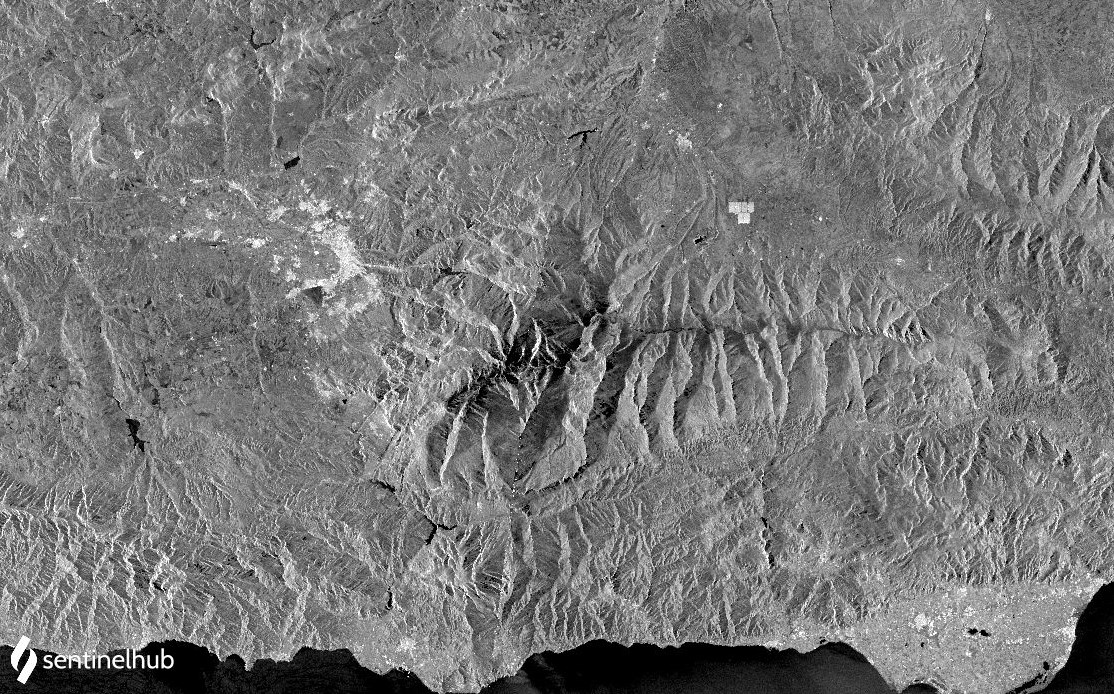
\includegraphics[width=.8\linewidth]{archivos/SAR_SN}
    \caption{Imagen \gls{sar} de Sierra Nevada tomada por el satélite de Sentinel-1 con polarización VV (dB). \cite{sentinelhub}}
    \label{fig:sar}
\end{figure}
\par La potencia recibida ($P_{R}$) se puede considerar como la contribución de los siguientes parámetros: potencia transmitida ($P_{T}$), longitud de onda ($\lambda$), ganancia de la antena ($G$), pérdidas en sistema ($L_{s}$) y en atmósfera ($L_{a}$), la longitud del trayecto ($R$), la superficie del área observada ($S$) y, por último, el coeficiente de backscattering ($\sigma_{0}$), teniendo en cuenta ambos trayectos de ida y vuelta y la propagación esférica de la onda, como se muestra en la fórmula \ref{Pr}. 
\\
\begin{equation} \label{Pr}
P_{R}=\frac{P_{T}\lambda ^{2}G^{2}\sigma_{0}S}{(4\pi ) ^{3}L_{s}L_{a}R^{4}}
\end{equation}
\\
\par Como podemos observar, el parámetro más interesante que nos va a dar información sobre la escena observada es el coeficiente de backscattering. Este parámetro es un valor adimensional (dB) que representa la relación entre la proporción de área equivalente si el objeto observado fuera un blanco isótropo (reflexión en todas direcciones por igual) ($m^{2}$) y su área o superficie observada real ($m^{2}$). Este parámetro va a depender de la frecuencia utilizada por el radar, la polarización de la onda, el ángulo de incidencia del pulso y del material y geometría de la superficie observada. Teniendo en cuenta solamente el coeficiente de backscattering y la longitud de onda empleada ($\lambda$), ya existen ciertos rangos que suelen representar distintos tipos de superficies observadas:
\begin{itemize}
	\item $\sigma_{0}$ > 0 dB: típicamente objeto artificial liso que está encarado al ángulo de incidencia del radar y actúa como un espejo.
	\item -10 dB < $\sigma_{0}$ < 0 dB: superficies muy rugosas como pueden ser vegetaciones densas donde hay mucha probabilidad de reflexión.
	\item -20 dB < $\sigma_{0}$ < -10 dB: superficies rugosas como vegetaciones menos densas entre las que se incluirían los cultivos. 
	\item $\sigma_{0}$ < -20 dB: superficies lisas que no encaran el haz de incidencia del radar por lo que reflejan casi todo a otra dirección, esto se da en masas de agua en calma, carreteras o suelos muy secos. 
\end{itemize}

\par Por otra parte, existen técnicas de detección más complejas que consideran también la información proveniente de la fase y la polarización para el desarrollo de modelos. Los principales son la interferometría, la interferometría diferencial y la polarimetría.
\\
\par Con el objetivo de maximizar la resolución espacial del área observada por el radar, esto es, la distancia mínima distinguible, se necesita mejorar la resolución en rango y en azimuth. La resolución en rango depende de la duración del pulso, ya que los objetos podrán ser diferenciados si están a una distancia mayor que un pulso, por lo que cuánto más pequeño sea este, mayor resolución de rango se obtendrá, aunque se debe mantener la duración del pulso para el rango de frecuencias asignado. Por otra parte, para mejorar la resolución en azimuth, se debe incrementar la resolución angular. Esta resolución es inversamente proporcional al ángulo de observación, ya que cuanto mayor es este, más objetos o áreas considera a la misma distancia y no es posible diferenciarlos. Para obtener ángulos pequeños se necesita un beam muy directivo, y ello se consigue con una apertura o longitud de antena grande. Es aquí donde entran los sistemas radar de los que se va a extraer la información para este proyecto, los \gls{sar}. Estos sistemas consiguen aumentar la resolución en azimuth, con una longitud de antena no muy grande, realizando un barrido en azimuth y posterior procesamiento para ampliar el área observada. Un ejemplo de este barrido se puede ver en la figura \ref{fig:sarb}.
\\
\begin{figure}[h]
    \centering
    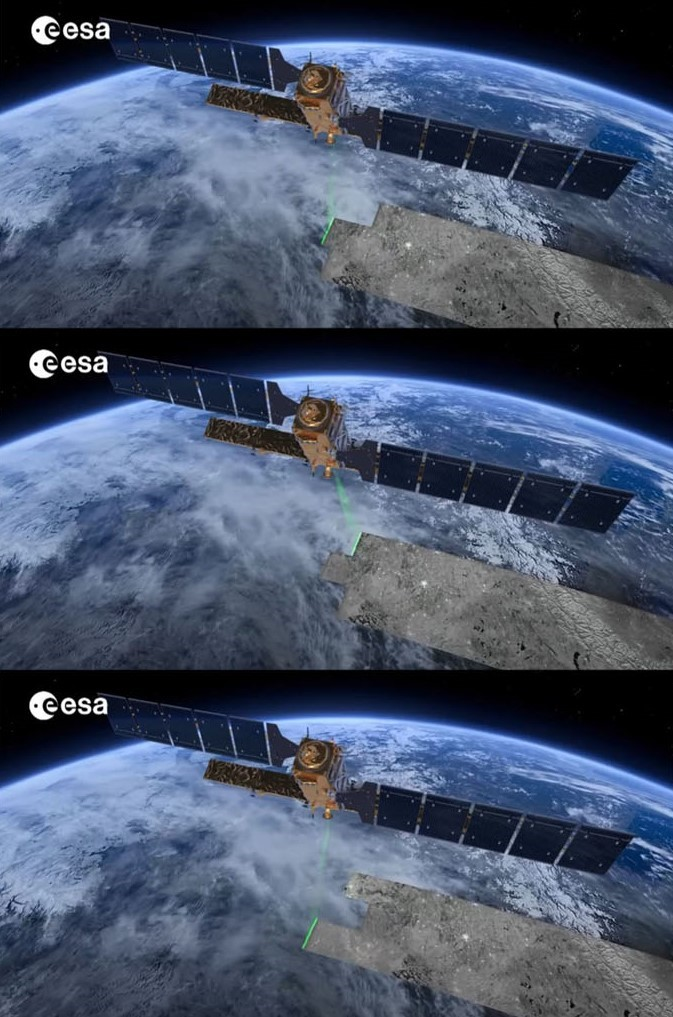
\includegraphics[height=12cm]{archivos/tfg/imgbarrido} % Tamaño de la imagen
    \caption{TOPS-SAR Sentinel-1 \cite{yts1}}
    \label{fig:sarb}
\end{figure}

\par Además de la resolución espacial, también existen otros parámetros que determinan la calidad de la información adquirida por los sistemas radar. Uno de ellos es el ruido que aparece como puntos de máximas y mínimas contribuciones debido a fenómenos puntuales que puede dificultar la interpretación de la información. Este ruido se denomina speckle, y la técnica utilizada para atenuar este efecto es la reducción por multi-look. Esta reducción se puede hacer realizando un filtrado paso bajo, que es la técnica más común, o tomando de varias imágenes de información de la misma área y el posterior promediado todas ellas, obteniendo así una información más plana, viéndose reducidos los píxeles de información aleatorios máximos y mínimos. 

\subsection{Procesamiento de imágenes SAR}
\par Las imágenes \gls{sar} pueden ser adquiridas con distintos formatos. El que se va a utilizar aquí es el formato \gls{grd}, con una resolución de 14m x 3m, por conveniencia para este estudio. Este formato consiste en imágenes \gls{sar} con multi-look (reducción de speckle) y proyectadas al rango de la tierra utilizando un modelo de elipsoide de la Tierra. La información de la fase es suprimida, lo cual no es un problema, ya que no era uno de los parámetros clave utilizados, y los píxeles que presenta la imagen son aproximadamente cuadrados \cite{copData}. 
\\
\par El primer problema reconocible en la obtención de estas imágenes es su falta de correspondencia con las coordenadas geográficas comúnmente utilizadas, además de las dimensiones y orientación de estas, ya que las imágenes abarcan áreas de mucho mayor tamaño a las áreas de cultivos aquí estudiados, y la orientación no es totalmente paralela al eje polar de la Tierra, sino que presenta cierta inclinación. Para solucionar todo ello, se realiza un pre-procesado utilizando el software libre SNAP cedido por la \gls{esa}, que se divide en los siguientes pasos:
\begin{enumerate}
	\item Lectura de las imágenes.
	\item Actualización de la información orbital en las imágenes cargadas.
	\item Cancelación de ruido térmico.
	\item Recorte del área de interés.
	\item Calibración radiométrica para obtener de salida de ambos canales (VH y VV) el formato $\sigma_{0}$.
	\item Filtrado de speckle.
	\item Conversión de escala lineal a dB.
	\item Geo-referenciación: genera un mapa en una rejilla uniforme de
coordenadas cartográficas con tamaño de píxel elegido de aproximadamente 10 m para cada coordenada (latitud y longitud).
	\item Escritura del producto en formato propio de SNAP: DEAM-DIMAP 
\end{enumerate}
\par Esto se realiza tantas veces como número de imágenes de distintas fechas se hayan obtenido. Para finalizar el procesamiento, se ajustan unas imágenes con otras para que todas estén referenciadas a las mismas coordenadas cartográficas en los mismos píxeles. Finalmente, estos píxeles tienen una resolución de 10m x 10m, debido a la degradación por el procesamiento. Una vez finalizado este proceso, las imágenes están preparadas para tratar su información información de manera más sencilla. 

\subsection{Satélites en teledetección}
\par Los sistemas \gls{sar} van a ser utilizados en este proyecto para observar parcelas cultivadas de la Tierra, por lo que los sistemas en los que se van a emplazar estos son los satélites. La misión satelital de la que se va a obtener información es Sentinel-1, del Programa Copérnico de la Comisión Europea y la \gls{esa}. Es una misión de órbita polar que engloba 2 satélites, A y B, cuyo objetivo es la observación de la superficie de la Tierra tanto terrestre como oceánica. Sentinel-1 concluyó sus lanzamientos de satélites en abril de 2016.  El rango de frecuencias de trabajo de Sentinel-1  proporciona información de la banda C, esto es entre 4-8 GHz, aunque, del mismo programa, la misión Sentinel-2 utiliza tecnología multiespectral, esto significa que trabaja en 13 bandas distintas, las cuales engloban la luz visible, el infrarrojo cercano y el infrarrojo de onda corta. Esto proporciona información más precisa y adecuada para cada fenómeno a observar \cite{copernicusOV}, lo cual puede ser utilizado para futuros avances de esta investigación. 
\\
\par La órbita se traza en el eje polar de la Tierra con una pequeña inclinación y sincrónica al Sol, una altitud de 693 km y un periodo de revista total de 6 días contando con ambos satélites, A y B, de Sentinel-1. En la figura \ref{fig:swath} se puede observar la órbita trazada por Sentinel-1 en un periodo de un día. Además, el sistema \gls{sar} no trabaja desde una posición perpendicular a la superficie terrestre a medir, ya que algunas superficies serían consideradas a la misma distancia por simetría en el swath, por lo que la visión del radar es lateral derecha. Esto deberá ser considerado para el procesamiento de extracción de información. 
\\
\begin{figure}[h]
    \centering
    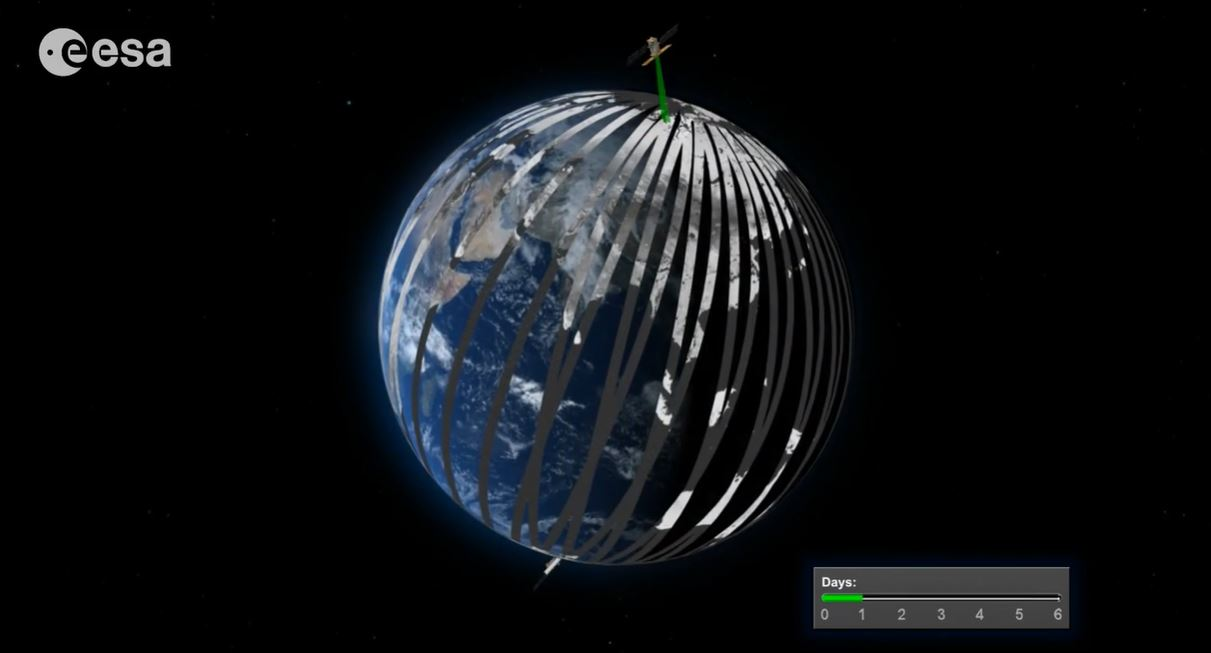
\includegraphics[width=.9\linewidth]{archivos/tfg/swathS1} % Tamaño de la imagen
    \caption{Swath a día 1 de 6 en Sentinel-1 \cite{ESAcons}}
    \label{fig:swath}
\end{figure}
\par Sentinel-1 tiene 4 modos de adquisición principales según el área que se pretende observar cuyos swath y resolución espacial varían. El primer modo, llamado Stripmap Mode, presenta un swath de 80 km y una resolución de 5x5 m. Este modo se utiliza para monitorización de islas pequeñas y emergencias puntuales. El segundo modo es Interferometric Wide Swath, de 250 km de swath y 5x20 m de resolución, es utilizado principalmente para todas las áreas de superficie terrestre, tanto áreas habitadas, como zonas montañosas o llanuras (donde se incluyen los cultivos). El tercer modo se conoce como Extra Wide Swath Mode, consta de un swath de 400 km y una resolución de 20x40 m, es utilizado para zonas marítimas, polares o cubiertas de hielo, donde se buscan grandes coberturas y un tiempo de revista corto, ya que, por el eje elegido para su órbita, las zonas polares se cubren en menor tiempo. Por último, cabe destacar el Wave Mode, cuyo swath se caracteriza por considerarse de superficie cuadrada de 20x20 km, y con una resolución de 20x5 m. Este es utilizado para la observación de los océanos \cite{EOSs1}. 
\\
\par Para que la utilización de estos modos sea posible, se necesita una tecnología \gls{sar} acorde con estas necesidades. El radar tiene unas dimensiones en Sentinel-1 de antena de 12.3 m x 0.821 m una vez desplegado. El rango del ángulo de incidencia con respecto a la Tierra es de 20 a 46 grados. Los modos de adquisición también pueden trabajar con distintas polarizaciones. Las ofrecidas por los satélites de Sentinel-1 para la emisión son Horizontal (H) y Vertical (V). Para la recepción se pueden elegir la misma polarización utilizada en emisión, lo que sería HH o VV, o recibir ambas polarizaciones independientemente de cuál haya sido enviada, HH+HV o VV+VH \cite{EOSs1}. Una emisión con polarización doble entorpecería el procesamiento ya que no se podría reconocer en la recepción qué parte de la señal correspondía a cada una. 


\section{Técnicas de regresión y Machine Learning}
\par Las técnicas de regresión proporcionan una estimación de una variable dependiente de otras la cual es útil para realizar predicciones, por lo que están relacionados con el aprendizaje automático o \gls{ml}. El \gls{ml} es un tipo de inteligencia artificial, que se caracteriza por la generación de un modelo estimado de manera automática por un computador. Esta estimación se realiza con un entrenamiento previo aplicado a un algoritmo de aprendizaje específico a una serie de datos de entrenamiento. Con este aprendizaje se elabora un modelo que es capaz de devolver una salida o solución a partir de unos parámetros de entrada que deben ser del mismo tipo que los utilizados en la fase de aprendizaje, el esquema general se puede ver en la imagen \ref{fig:ml}. 
\\
\begin{figure}[h]
    \centering
    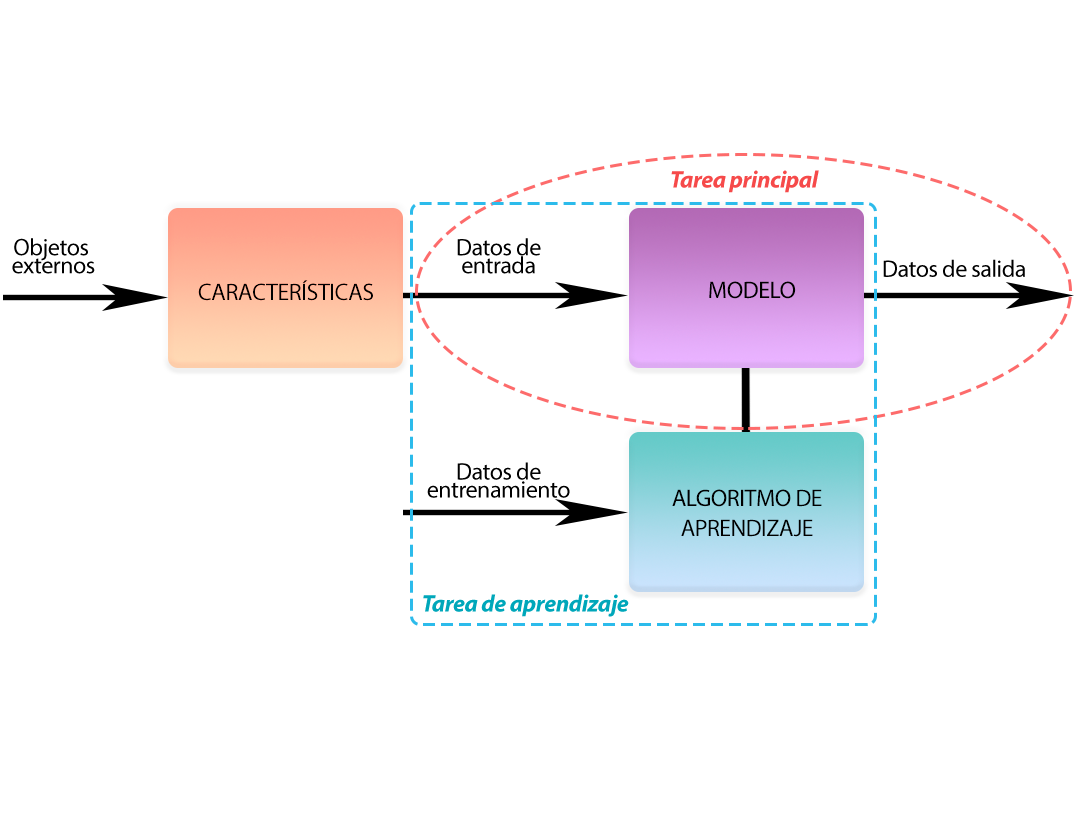
\includegraphics[width=.9\linewidth]{archivos/ESQUEMA_ML}
    \caption{Esquema general del funcionamiento de las técnicas de \gls{ml}.}
    \label{fig:ml}
\end{figure}
\\
\par Finalmente, el objetivo de las técnicas de \gls{ml} puede ser clasificar una información o realizar una previsión acorde con un modelo estimado. Como se puede ver, el objetivo de este y de las técnicas de regresión pueden coincidir para el segundo caso, y esto lleva a un desarrollo conjunto de ambas técnicas. 

\subsection{Clasificación de técnicas de Machine Leaning}
\par Los modelos empleados en \gls{ml} son numerosos, y su clasificación se puede realizar dependiendo de su algoritmo de aprendizaje y del tipo de razonamiento en el que se basa. Comenzando por la clasificación según su algoritmo de aprendizaje, que principalmente se dividen según el feedback  del que aprenden, los modelos se pueden clasificar de la siguiente manera \cite{MLRussell}: 
\begin{itemize}
	\item Aprendizaje no supervisado: este aprendizaje se basa en la clasificación o agrupación de los objetos de entrada según patrones que cumplen las distintas entradas de estos. Estos métodos no devuelven un nombre específico para cada grupo o cluster ya que no se le han proporcionado referencias o etiquetas en la etapa de entrenamiento. Necesita numerosas entradas en el entrenamiento para detectar patrones suficientemente estables. 
	\item Aprendizaje por refuerzo: el aprendizaje se realiza por refuerzo positivo, que sería una recompensa, o negativo, penalización. Este algoritmo buscaría la estimación del modelo para obtener el máximo refuerzo positivo posible. Así, tras suficiente entrenamiento construye un modelo muy preciso para nuevas entradas. 
	\item Aprendizaje supervisado: tanto las entradas como las salidas están previamente definidas en la etapa de aprendizaje. Se realiza un entrenamiento en el que se utilizan las entradas con sus correspondientes salidas para elaborar el modelo. Una vez suficientemente entrenado, este puede obtener salidas previamente desconocidas a partir de entradas similares a las del entrenamiento. Los resultados están limitados a los proporcionados en la etapa de entrenamiento, pero estos suelen ser más estables con menos cantidad de datos que otros modelos. 
	\item Aprendizaje semi-supervisado: este aprendizaje recibe algunas de sus entradas correctamente etiquetadas y el resto de ellas, la mayoría, sin etiquetar, así tiene algunas referencias para la clasificación fiables pero no toma las etiquetas como una referencia totalmente cierta para toda la clasificación como ocurre en el aprendizaje supervisado. Así se evitan malos aprendizajes por ruido o etiquetas erróneas en los datos de entrada. Bastante común en grandes masas de datos para aprendizaje. 
\end{itemize}
\par Por otra parte, teniendo en cuenta la base de los razonamientos internos que los algoritmos realizan para obtener las salidas correspondientes, aunque no considerando esta división estricta, las técnicas se pueden clasificar de la siguiente manera \cite{MLFlach}:
\begin{itemize}
	\item Geométricos: los modelos geométricos son aquellos cuyos objetos pueden ser representados en un espacio de instancias (X) en el que cada instancia corresponde a un posible objeto, esto es, habrá tantas instancias como objetos con distintas combinaciones de entradas posibles. Por otra parte, las etiquetas también se representan como un espacio de etiquetas (Y) con un número finito de posibilidades \citep{MLPref}. Utilizando estos conceptos, el algoritmo se desarrolla con otros conceptos geométricos como son líneas, planos y distancias. Estos métodos suelen ser aplicados cuando X e Y están formados por valores numéricos, que son fácilmente representables en ejes de coordinadas.
	\item Probabilísticos: los modelos probabilísticos parten de la base de que las entradas de los objetos están basadas en un proceso aleatorio que hacen referencia a una distribución de probabilidad desconocida. Se busca definir esa distribución P(Y|X), siendo X el conjunto de objetos posibles e Y las etiquetas correspondientes. Aquí el modelo tendría como salidas probabilidades para cada una de las opciones posibles. 
	\item Lógicos: los modelos lógicos son los más cercanos al razonamiento humano y los más comprensibles también como algoritmos. Se basan en decisiones lógicas, estructuradas típicamente en forma de árbol, esto es llamado árbol de decisiones y según las características de los parámetros de entrada nos vamos desplazando hacia la base del árbol, obteniendo al final una única salida para cada objeto de entrada. 
	\item Agrupaciones y gradiente: estos modelos se incluyen en los anteriores, ya que es una clasificación paralela según el tratamiento del espacio de instancias (X): agrupaciones seccionando estos espacios en un número de segmentos definido, fácilmente representables y con una única solución, en cambio; en los gradientes, no existe una segmentación previamente definida, por lo que el modelo trata todo el espacio como uno solo. 
\end{itemize}

\subsection{Modelos de Machine Learning}
\par Una vez presentadas todas las posibles clasificaciones de técnicas de \gls{ml}, podemos adentrarnos en los modelos más comunes, a qué tipo de los anteriores pertenecen y algunas aplicaciones. Algunos de los más conocidos son los siguientes:
\begin{itemize}
	\item Redes neuronales artificiales: este modelo es de tipo geométrico y de aprendizaje supervisado, ya que el entrenamiento consta de entradas etiquetadas con su correspondiente salida. Este modelo se caracteriza por estar inspirado por las redes neuronales naturales del cerebro animal, obteniendo resultados sin unas reglas preestablecidas de análisis. Estas redes están compuestas por capas de neuronas, las cuales representan un peso y una función de activación por la que una parte de la información de entrada se va a procesar. Estas funciones y pesos se van ajustando mediante el entrenamiento hasta tener una red óptima para su funcionamiento. En cuanto a aplicaciones, la más común es el reconocimiento en imágenes de objetos o caracteres.
	\item Máquinas de vectores de soporte: es un modelo geométrico y supervisado. Este modelo utiliza el espacio de instancias para representar los objetos de entrenamiento como puntos y las salidas como líneas o hiperplanos, dependiendo del número de dimensiones. Una vez ajustado este modelo, las nuevas entradas se clasificarán según al espacio al que pertenezcan. Este modelo está muy relacionado con la clasificación/agrupación y la regresión. Algunas de sus aplicaciones son la clasificación de textos \citep{MLText} o, el más interesante para este proyecto, la clasificación de información procedente de un \gls{sar} \citep{MLSAR}.
	\item Redes bayesianas: es un modelo probabilístico y gráfico, a la vez que lógico, de aprendizaje supervisado. Se basa en un modelo gráfico de nodos que corresponden a variables conocidas o desconocidas y el tratamiento probabilístico simplificado con la regla de la cadena. Son muy utilizadas en aplicaciones relacionadas con las ciencias de la salud para modelar comportamientos biológicos. 
	\item Árboles de decisión: es un modelo lógico y de aprendizaje supervisado. Es uno de los modelos lógicos más ilustrativos porque se basa en árboles que siguen las reglas de decisión, yendo desde el primer nodo de decisión donde se sitúa la entrada resolviendo condiciones de estas hasta llegar a una única salida o nodo terminal, alcanzable por un camino único, que es la salida del modelo, así se puede ver en el esquema de ejemplo de la figura \ref{fig:arbol}. En el aprendizaje, este modelo va ajustando sus condiciones y elaborando el árbol más coherente para llegar a las soluciones necesarias. Este método es bastante sencillo de implementar y comprender. Relacionado con ese modelo también encontramos el conocido como \gls{rf}. Este modelo se caracteriza por generar numerosos árboles de decisión provenientes de un factor aleatorio con la misma distribución. Al obtener los resultados de cada uno de los árboles, se realiza un promediado, tomando la respuesta más repetida como la más probable pero teniendo la posibilidad de considerar el resto de salidas en su correspondiente porcentaje. De esta manera, un modelo que era limitado a una respuesta única, se abre devolviendo una respuesta probabilística. Este tipo de respuesta es especialmente interesante para la inclusión de estas estimaciones con datos de otros modelos predictores, ya que no excluye el resto de estimaciones. 
	\item Las técnicas de regresión: son todas aquellas técnicas, típicamente de aprendizaje supervisado, que buscan la relación de una variable dependiente con una o más variables independientes mediante la estimación de su función de regresión. Para ello se consideran y ponderan todos los valores de la variable dependiente para unos valores fijos de las variables independientes. Además, en estos análisis, también se puede tener en cuenta la varianza de la variable dependiente para estos mismos valores, pudiendo ser estudiada también mediante su distribución de probabilidad. Esta varianza indica la fiabilidad de nuestras estimaciones o el ``ruido'' en las medidas de la variable dependiente. En general, estas técnicas ajustan una función de regresión, por lo que se aplican cuando las variables tienen sentido numérico. Además, estas pueden ser combinadas con otros modelos, como los conjuntos de árboles de decisiones de regresión, conocido como \gls{rfr}.
\end{itemize}

\begin{figure}[h]
    \centering
    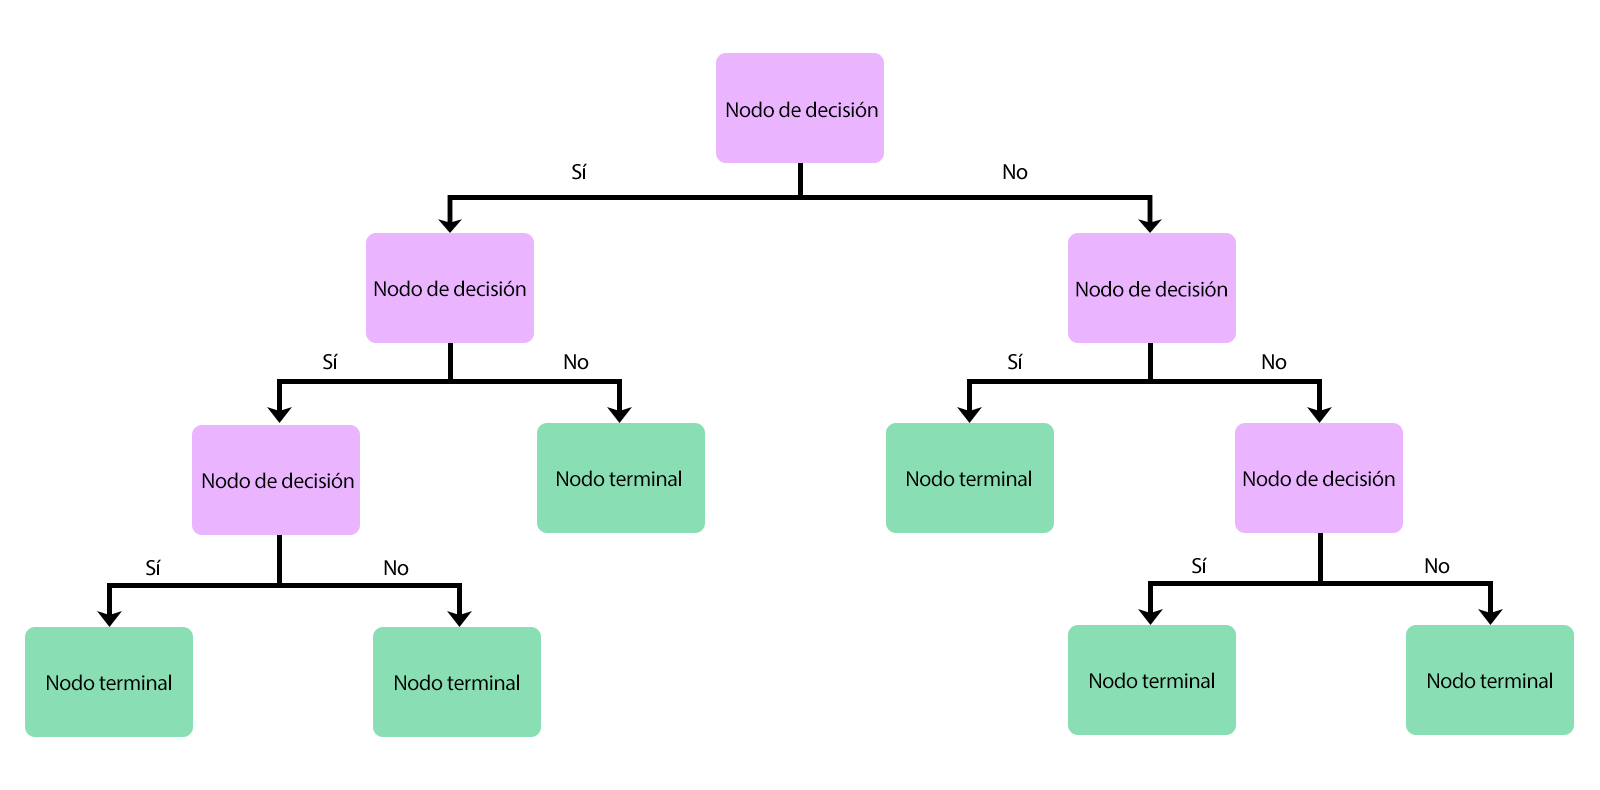
\includegraphics[width=\linewidth]{archivos/arb_des}
    \caption{Ejemplo de esquema de árbol de decisiones.}
    \label{fig:arbol}
\end{figure}

\par Ya que las técnicas de regresión pretenden modelar una función para una variable, a partir de otras conocidas, este va a ser el método más conveniente para realizar las predicciones del estado fenológico de los cultivos. El caso más sencillo de regresión es en el que solo tenemos una variable dependiente y otra independiente, este caso se conoce como regresión lineal simple, ya que la función de regresión estimada se corresponde a una ecuación lineal de una recta. Los datos que obtenemos para la variable dependiente que vamos a relacionar tienen, aparte de las componentes lineales, una componente aleatoria de ruido que puede deberse a distintos fenómenos como la precisión mínima del instrumento de medida, el ruido que este mismo genera en la medida o contribuciones de fuentes externas, consideradas como ruido también. Esta función de regresión es frecuentemente estimada mediante el \gls{mmc}. También existe la regresión lineal múltiple, que funciona de la misma manera pero con mayor número de variables independientes, por lo que en lugar de una recta, la función de regresión representa un plano en el que coinciden N dimensiones, siendo N el número de variables independientes total. Su expresión analítica se presenta en la ecuación \ref{RL}, donde $Y$ corresponde a la variable dependiente, $X$ a las variables independientes, $\beta$ parámetro de influencia de cada variable independiente, y $\varepsilon$ el término aleatorio.
\\
\begin{equation} \label{RL}
Y_{t}=\beta _{0}+\beta _{1} X_{1}+\beta _{2} X_{2}+...+\beta _{N} X_{N}+\varepsilon 
\end{equation}
\par Cuando la función de regresión no es una función lineal, la regresión es no lineal, ya que la respuesta de la variable dependiente puede ser exponencial, logarítmica o polinomial, entre otras, por lo que la función de regresión presentará mayor complejidad. Aquí también es común utilizar el \gls{mmc} o la regresión segmentada, que ajusta como regresión lineal segmentos de la original no lineal.
\\
\par Cualquier variable independiente que tenga relación con la dependiente es útil en mayor o menor medida pero siempre proporciona información aunque su varianza sea muy grande o su contribución relativamente pequeña. Cualquier tipo de información extra proporciona un ajuste a la estimación final positivo si esta se ha modelado correctamente. 
\\
\par A parte de las regresiones lineales y no lineales mencionadas, también encontramos otros métodos de regresión como son los mínimos errores absoluto (bastante similar al \gls{mmc}), la regresión no paramétrica o la regresión lineal bayesiana.

\section{Estimación de parámetros físicos de cultivos mediante teledetección}

\par La fenología es la ciencia que estudia la relación entre los factores climáticos y los ciclos de los seres vivos \citep{feno}. Esto es, el estudio del desarrollo de plantas y animales en relación con parámetros ambientales. Este proyecto se centra en el estudio fenológico de plantas, en concreto de cultivos de arroz.
Por lo que, a continuación, se van a presentar los conceptos físicos que definen el estado de desarrollo de estos cultivos, para comprender cuáles son los parámetros clave y utilizados en el marco de investigación. Una vez introducidos, se expone el concepto de la técnica utilizada hasta el momento, los modelos de evolución y observación. Por último, se verá la aplicación de las técnicas de regresión a los datos obtenidos para elaborar un modelo representativo del estado fenológico de un cultivo.
\\
\par Algunos de los parámetros descriptores clave utilizados en el marco creado de este proyecto son los siguientes: 
\begin{itemize}
	\item Escala \gls{bbch}, que recibe su nombre por los participantes en su estudio y desarrollo, es una escala numérica de intervalo 0-9 que describe la fenología \cite{bbch}. Cada valor numérico corresponde a un estado de desarrollo, desde la germinación o primeros brotes, correspondientes al estado 0, hasta la senectud, estado 9. Cada estado puede estar dividido hasta en 10 sub-etapas. El rango de que cada etapa abarca, concretamente para los cultivos de arroz, se puede observar en la tabla \ref{bbch_rice}. Para que uno de estos estados sea considerado el nivel general de una parcela, no solo tiene que ser este estado el mayoritario, sino que debe abarcar más del 50\% del cultivo. 
	\item \gls{ndvi}, es un observable proporcionado por los sensores ópticos que suele ser usado para estimar la cantidad, calidad y desarrollo de la vegetación con base a la medición de la intensidad de la radiación de ciertas bandas del espectro electromagnético en ella. Estas bandas son concretamente las bandas del rojo y del infrarrojo cercano, con rangos de  reflexión entre 0 y 1 cada una de ellas. El coeficiente \gls{ndvi} se obtiene según la fórmula \ref{eq:ndvi}, conformando un rango entre -1 y 1, y representa el desarrollo de la vegetación, ya que la contribución de la banda infrarroja cercana está ligada a la reflexión de la celulosa, por tanto a las áreas verdes y frondosas, mientras que la banda roja es mucho menos sensible a estas contribuciones y más a la absorción de clorofila. En resumen, un buen desarrollo vegetal tiene valores de \gls{ndvi} más cercanos a la unidad positiva \citep{ndvi}. 
	\begin{equation} \label{eq:ndvi}
		NDVI = \frac{IRCercano-ROJO}{IRCercano+ROJO}
	\end{equation}
	\item Temperatura del aire, o el calor acumulado durante todo el proceso de desarrollo de un cultivo, es una fuente de observaciones para el que existen modelos de observación que lo relacionan con el estado fenológico. Concretamente en los cultivos de arroz tiene un impacto notable, por lo que se considera otro de los parámetros a tener en cuenta en su monitorización y en la elaboración de modelos de predicción \cite{Juanma2016}.
\end{itemize} 

\begin{longtable}{p{3cm}p{1cm}p{9cm}}
%\centering
%\begin{tabular}{p{.20\textwidth}p{.20\textwidth}p{.20\textwidth}}
\multicolumn{1}{c}{Estado de crecimiento} & BBCH & \multicolumn{1}{c}{Descripción}                                                                                                          \\ \hline
Germinación                             & 00   & Semilla seca                                                                                                                             \\
                                           & 01   & Comienzo de la imbibición de semillas                                                                                                    \\
                                           & 03   & Imbibición de semillas completada                                                                                                        \\
                                           & 05   & Emerge radícula de la cariopsis                                                                                                          \\
                                           & 06   & Elongación de la radícula y raíz visible                                                                                                 \\
                                           & 07   & Emerge coleóptilo de la cariopsis                                                                                                        \\
                                           & 09   & Emergen hojas imperfectas aún enrolladas en la parte superior del caleóptilo                                                             \\ \hline
Desarrollo de las hojas                    & 10   & Desenrollamiento de las hojas imperfectas y primera hoja real visible                                                                    \\
                                           & 11   & Primera hoja real desenrollada                                                                                                           \\
                                           & 12   & 2 hojas reales desenrolladas                                                                                                             \\
                                           & 13   & 3 hojas reales desenrolladas                                                                                                             \\
                                           & 19   & 9 o más hojas desenrolladas                                                                                                              \\ \hline
Vástagos                                   & 21   & Primer vástago detectable                                                                                                                \\
                                           & 22   & 2 vástagos detectables                                                                                                                   \\
                                           & 23   & 3 vástagos detectables                                                                                                                   \\
                                           & 29   & Máximo número de vástagos detectables                                                                                                    \\ \hline
Elongación de tallo                        & 30   & Inicio de la panícula o etapa del anillo verde: la clorofila se acumula en el tejido del tallo, formando un anillo verde                 \\
                                           & 32   & Formación de panícula: panícula de 1–2 mm de largo                                                                                       \\
                                           & 34   & Etapa de alargamiento: los entrenudos comienzan a alargarse, la panícula mide más de 2 mm de largo (dependiendo de la variedad)          \\
                                           & 37   & Última hoja visible todavía enrollada y panícula moviéndose hacia arriba                                                                 \\
                                           & 39   & Última hoja desenrollada: aurícula y lígula de la última hoja y penúltima hoja alineada (etapa previa al arranque)                       \\ \hline
Arranque                                   & 41   & Etapa inicial de arranque: parte superior del tallo ligeramente engrosada, vaina de la hoja de bandera a unos 5 cm de la penúltima vaina \\
                                           & 43   & Etapa media de arranque: vaina de la última hoja a 5–10 cm de la penúltima vaina de la hoja                                              \\
                                           & 45   & Etapa de arranque tardía: vaina de la última hoja hinchada y a más de 10 cm de la penúltima vaina de la hoja                             \\
                                           & 47   & Abertura de la vaina de la última hoja                                                                                                   \\
                                           & 49   & Vaina de hoja de bandera abierta                                                                                                         \\ \hline
Aparición de inflorescencia                & 51   & Comienzo de la emergencia de la panícula: la punta de la inflorescencia emerge de la vaina                                               \\
                                           & 52   & 20\% de la panícula emergida                                                                                                             \\
                                           & 53   & 30\% de la panícula emergida                                                                                                             \\
                                           & 54   & 40\% de la panícula emergida                                                                                                             \\
                                           & 55   & Mitad de la panícula emergida: nodo del cuello todavía en vaina                                                                          \\
                                           & 56   & 60\% de la panícula emergida                                                                                                             \\
                                           & 57   & 70\% de la panícula emergida                                                                                                             \\
                                           & 58   & 80\% de la panícula emergida                                                                                                             \\
                                           & 59   & Fin de la emergencia de la panícula: nivel del ganglio del cuello con la aurícula de la hoja bandera, anteras aún no visibles            \\ \hline
Florecimiento                              & 61   & Comienzo de la floración: anteras visibles en la parte superior de la panícula                                                           \\
                                           & 65   & Floración completada: anteras visibles en la mayoría de las espiguillas                                                                  \\
                                           & 69   & Fin de la floración: todas las espiguillas han completado la floración, pero algunas anteras deshidratadas pueden permanece              \\ \hline
Desarrollo del fruto                       & 71   & Maduración acuosa: los primeros granos han alcanzado la mitad de su tamaño final                                                         \\
                                           & 73   & Cosecha temprana                                                                                                                         \\
                                           & 75   & Cosecha media: contenido del grano lechoso                                                                                               \\
                                           & 77   & Cosecha tardía                                                                                                                           \\ \hline
Maduración                                 & 83   & Masa temprana                                                                                                                            \\
                                           & 85   & Masa blanda: contenido de grano suave pero seco, granos y glumas aún verdes                                                              \\
                                           & 87   & Masa dura: contenido de grano sólido                                                                                                     \\
                                           & 89   & Completamente maduro: grano duro, difícilmente divisible manualmente                                                                     \\ \hline
Senescencia                                & 92   & Sobre-maduro: grano muy duro, no puede ser abollado manualmente                                                                          \\
                                           & 97   & Planta muerta y colapsando                                                                                                               \\
                                           & 99   & Producto cosechado                                                                                                                     
                                           
%\end{tabular}
%\caption{Escala \gls{bbch} identificativa de los estados de desarrollo del arroz. \cite{bbcht}\label{bbch_rice}}
\end{longtable}

\subsection{Metodología general basada en espacio de estados}
\par En este área hay estudios previos donde se crea la metodología basada en espacio de estados utilizada. El primer artículo \cite{Juanma2014} de este marco de trabajo, de 2014, trata de estimar el estado fenológico de cultivos en tiempo real empleando espacio de estados y técnicas de sistemas dinámicos utilizando información del pasado y actualizaciones. Esto se ve representado por dos modelos diferenciables, los cuales son el modelo de evolución: modelo que predice el estado fenológico de un cultivo según el desarrollo cronológico típico del mismo, y el modelo de observación: modelo que trata de predecir el estado de fenológico a partir de variables físicas observables. Estos modelos son combinados para considerar tanto el desarrollo habitual de un cultivo como posibles variaciones temporales (adelantos o retrasos) en el mismo que pueden ser debidos a múltiples factores. 
\\
\par Dentro del espacio de estados se define que cada etapa de la evolución corresponde a un único estado, el cual está contenido en un sistema dinámico o proceso, ya que tiene una evolución temporal. Este sistema se define según las siguientes ecuaciones, donde la fórmula \ref{eq:xt} es el proceso recursivo, correspondiente al modelo de evolución, y la fórmula \ref{eq:zt} es la ecuación de medida, que relaciona una nueva observación con el sistema, por lo que corresponde al modelo de observación.
\\
\begin{equation} \label{eq:xt}
\dot{x}(t) = \frac{dx(t)}{dt}=f(x(t),t,v(t))
\end{equation}
\begin{equation} \label{eq:zt}
z(t) = h(x(t),t,w(t))
\end{equation}
\par El vector de estados $x(t)$ es el vector de $n$ variables de estado que describe el sistema en un momento determinado $t$, por lo que el espacio de estados dispone de $n$ dimensiones. Las funciones que aportan el régimen de cambio para cada estado está representado por $f()$ y el ruido en la evolución es $v(t)$. $z(t)$ representa el vector de salida, donde $w(t)$ es el ruido, y $h(t)$ la relación entre el vector de estados y la observación $z(t)$.
\\
\par Las dos etapas en las que se divide este algoritmo son predicción y actualización. La actualización se produce cuando existe información observable nueva, esta se introduce al sistema mediante un filtro extendido de Kalman y genera un nuevo estado y una matriz de transiciones, la cual representa la probabilidad de los siguientes posibles estados.
\\
\par Para la creación del modelo de evolución se utilizan los mismos observables polarimétricos (información del radar polarimétrico, vertical (V) y horizontal (H), del satélite Radarsat-2) que para las actualizaciones. Los valores de este modelo no son exactamente la escala \gls{bbch} ya que no hay un registro continuo para ello pero están discretizados y agrupados en rangos equivalentes a valores fenológicos. Estas agrupaciones o clusters van ajustando su centro con las actualizaciones de los observables. La estimación, entonces, se realiza combinando la información de este modelo, una vez que está generado y conociendo la información temporal del cultivo a estimar, con la información observable por medio del \gls{ekf}.
\\
\par En 2016, el mismo grupo publicó otro artículo \cite{Juanma2016} en el que se trata de estimar la fenología de cultivos de arroz a partir de dos fuentes de información observables: imágenes \gls{sar} del satélite TerraSAR-X y temperatura del aire registrada, combinadas en tiempo real mediante filtros de partículas. Se mantiene el método de trabajo de espacio de estados con predicción y actualización. 
\\
\par Además de las mejoras que presenta por la consideración de la temperatura como fuente de información, este artículo introduce cómo trabajar con las imágenes \gls{sar}. Las imágenes \gls{sar} dan una información del coeficiente de reflexión de la superficie observada, según una polarización de onda emitida y recibida, siendo este representado en ejes de azimuth y rango, como se ha explicado anteriormente. Estas imágenes, proporcionadas por la \gls{esa}, cuentan con canales de polarización VV y HH para TerraSAR-X y VV y VH para Sentinel-1, esto último es, emisión vertical y recepción tanto vertical como horizontal. La segunda configuración es más sensible al crecimiento de los cultivos de arroz por la verticalidad de sus tallos. Por otra parte, las imágenes de polarización horizontal recibida proporciona información extra que puede ser útil y que es bastante semejante a la obtenida en HV, es decir, emisión horizontal y recepción vertical, por lo que se abarca la mayor parte de información útil posible. A parte de las distintas polarizaciones, las imágenes \gls{sar} obtenidas por el satélite TerraSAR-X son equivalentes a las obtenidas por Sentinel-1, por lo que su marco de trabajo es perfectamente compatible. 


\subsection{Regresión aplicada a la estimación}
\par Dentro del marco de trabajo previo, este \gls{tfg} se va a centrar en elaborar un modelo de observación a partir de las imágenes \gls{sar} de satélite para cultivos de arroz, haciendo uso de la regresión de series temporales y técnicas de aprendizaje automático. Modelo que posteriormente se combina con el de evolución para la elaboración de estimaciones más completas y fiables. La regresión busca generar un modelo de predicción del fenómeno que se está estudiando a partir de una información de la que el fenómeno depende. En este caso, ese fenómeno es el estado fenológico de los cultivos de arroz y la información a partir de la cuál se va a generar este modelo son los coeficientes de backscattering obtenidos para las distintas polarizaciones (VV y VH), su cociente y la desviación estándar de cada uno, todo ello a nivel de media de parcela y día.
\\
\par A la hora de crear un modelo a partir de regresión, se debe considerar la evolución que se quiere estudiar para elegir la información que se va a utilizar. Para el estudio de la fenología se debe escoger información que complete un periodo de desarrollo desde el primer estado de la siembra del cultivo, hasta la madurez y recogida del producto, información que debe presentar una resolución temporal suficiente para que sean distinguibles las distintas etapas dentro del proceso. A esto se suma que para la generación de un modelo fiable este tiene que ajustarse con un número determinado de ciclos enteros de información, en mayor o menor número dependiendo de la fiabilidad y constancia de los mismos. 
\\
\par Habiendo generado un modelo utilizando técnicas de regresión, este debe ser comparado con información contrastada de los cultivos que indiquen si el modelo se aproxima lo suficiente a la realidad del terreno y, por tanto, es un modelo fiable. Esto significaría que la información utilizada, a priori, tiene relación con el fenómeno estudiado, y que la cantidad de información ha sido suficiente para ajustar el modelo, por lo que puede ser utilizado para predicción, en este caso, del estado fenológico del nuevo cultivo observado. 
\\
\par En este modelo no se incluye la parte dinámica del sistema, ya que esta está representada en el modelo de evolución y, por tanto, en la unión de ambos modelos. Pero este modelo se genera únicamente a partir de los observables anteriormente mencionados. Las salidas de este modelo son funciones de densidad de probabilidad (\gls{pdf}) del estado fenológico del cultivo combinables con las salidas del modelo de evolución. 	% Plantilla: Se muestran listas
\input{capitulos/objetivos}		% Plantilla: Se muestran tablas
 %%%%%%%%%%%%%%%%%%%%%%%%%%%%%%%%%%%%%%%%%%%%%%%%%%%%%%%%%%%%%%%%%%%%%%%%
% Plantilla TFG/TFM
% Escuela Politécnica Superior de la Universidad de Alicante
% Realizado por: Jose Manuel Requena Plens
% Contacto: info@jmrplens.com / Telegram:@jmrplens
%%%%%%%%%%%%%%%%%%%%%%%%%%%%%%%%%%%%%%%%%%%%%%%%%%%%%%%%%%%%%%%%%%%%%%%%

\chapter{Metodología}
\label{metodologia}
\par El desarrollo de este \gls{tfg} va a consistir en la creación de un script de Python que tenga como entradas los datos de \gls{sar} de Sentinel-1, y como salida la función de densidad de probabilidad para la \gls{bbch} y/o altura de la planta, utilizando \gls{rfr} para realizar esta estimación. 
\\
\par Los datos de entrada de satélite de los que disponemos constan de las 7 parcelas de arroz sobre las que se trabaja: Calogne, Ermita, Puntal, Mínima, Puebla, Reboso y Vega, y los valores en dB del coeficiente de backscattering para polarizaciones VV y VH, obtenidos de las imágenes \gls{sar}, con periodo de revista de 6 días. Para realizar el modelo de observación necesitamos contrastar con datos reales de los cultivos utilizados, por lo que se dispone también de los siguientes datos de las 7 parcelas para los años 2017 y 2018: su posición geográfica, área, días de siembra y de cosecha, producción, \gls{bbch} total, mínima y máxima, la altura media del cultivo y los días del año para los cuales se han tomado estos datos. De todos ellos, los más relevantes para este estudio son la \gls{bbch} por parcela, la altura del cultivo y los días de siembra, cosecha y de toma de datos, los cuáles no tienen porqué coincidir con el periodo de revista de los satélites de Sentinel-1.
\\
\par  El procesamiento que los datos de satélite necesitan para la elaboración del modelo es distinto dependiendo del método utilizado. En este proyecto se realizan pruebas para la estimación de 3 casos de salidas distintas: \gls{bbch}, altura (cm) y \gls{bbch} junto a altura (cm). Además, cada uno de estos casos se evalúa utilizando los datos de entrada a nivel de parcela (mediante la media) y a nivel de pixel, desconociendo a priori qué método obtiene mejores resultados. Para ambos métodos, el procesamiento de los datos comienza restringiendo la información al periodo que nos interesa: desde el día de siembra hasta el de cosecha. A continuación, se ajustan los días de los que se tiene información realizando una interpolación para los datos de \gls{bbch} y/o altura, haciéndolos coincidir con las fechas de toma de datos del satélite, cuyos datos no deben interpolarse ya que su evolución no es tan creciente lineal como la altura o la fenología. El siguiente procesamiento se da únicamente para el método a nivel de parcela: se realiza la media y la desviación estándar de los datos que vamos a utilizar como entradas del sistema (VV en dB, VH en dB, y el ratio entre ambos, VH-VV, también en dB). Para finalizar la preparación de los datos, se dividen estos en sets de entrenamiento y de test. La división se realiza por parcelas completas, para que sea más sencillo y completo su entrenamiento y posterior visualización. Para todos los casos se reservan 6 parcelas de entrenamiento y 1 de test de resultados. Los datos reales con los que se va a entrenar y examinar el modelo se preparan con la interpolación mencionada anteriormente y la división de parcelas que sigue los mismos requisitos que los datos de satélite. La única adaptación extra que tienen estos datos se da en el caso de nivel de pixel: como no contamos con la información medida en tierra a ese nivel de \gls{bbch} ni de altura, los valores generales para cada parcela interpolados deben ser asignados a cada uno de los píxeles correspondientes de esa parcela, es decir, todos los píxeles tendrán el mismo valor de salida para una misma parcela y día. Una interpretación gráfica aproximada de este procesamiento se puede ver en la figura *INSERTAR CROQUIS*.
\\
\par Una vez procesados todos los datos y creados los sets de entrenamiento y test, estos datos pueden ser guardados y cargados para no repetir el procesamiento en futuras ocasiones. A continuación, la implementación del regresor, su entrenamiento y evaluación completa la creación del modelo de observación y este está listo para realizar predicciones. En la creación del modelo existen distintos parámetros modificables según la técnica de \gls{rfr} para optimizarlo acorde con las características del problema que se intenta resolver. El número de estimadores o número de árboles es uno de los principales parámetros, por defecto 100, el cual va representar el número de árboles de decisión de los que se va a componer el regresor. Mayor número de árboles implica una mayor complejidad y la posibilidad de generar soluciones más profundas y precisas, con el riesgo de hacer un sistema excesivamente complejo que tenga sobreajuste u overfitting en su entrenamiento y que tenga un costo computacional muy elevado sin realmente aportar mejoras significativas. Otros parámetros variables en la creación del regresor, ya dentro de los árboles de decisión, son la profundidad máxima (número máximo de nodos y niveles de cada árbol, por defecto nulo), el mínimo número de muestras para dividir un nodo interno (por defecto 2), el número mínimo de muestras para un nodo final (por defecto 1) o estado aleatorio inicial en la creación de los árboles de decisión (por defecto nulo), entre otros. Debido a las características de nuestro sistema, se mantienen los valores por defecto de todos los parámetros excepto el número de estimadores y el estado de aleatoriedad, parámetros que se destinan a la optimización del regresor ya que son los más influyentes en los resultados finales. 
\\
\par La optimización del número de estimadores se realiza ejecutando una prueba para todas las posibilidades entre los valores 1 y 1000 y escogiendo el valor mínimo de estimadores que presente un máximo local no puntual del error cuadrático, es decir, al que tiende de manera progresiva, y con una mejora considerable. La optimización del estado de aleatoriedad se realiza de la misma manera. Este último parámetro también garantiza una generación aleatoria similar para los mismos parámetros independientemente de las veces que se realicen las pruebas, esto es, la ``semilla'' de la que parte esta generación es la misma, por lo que se puede realizar una evaluación fiable de los resultados, ya que no van a depender de cómo se hayan generado inicialmente los árboles de decisión. 	% Plantilla: Se muestran figuras
\input{capitulos/desarrollo}		% Plantilla: Se muestran listados
%%%%%%%%%%%%%%%%%%%%%%%%%%%%%%%%%%%%%%%%%%%%%%%%%%%%%%%%%%%%%%%%%%%%%%%%
% Plantilla TFG/TFM
% Escuela Politécnica Superior de la Universidad de Alicante
% Realizado por: Jose Manuel Requena Plens
% Contacto: info@jmrplens.com / Telegram:@jmrplens
%%%%%%%%%%%%%%%%%%%%%%%%%%%%%%%%%%%%%%%%%%%%%%%%%%%%%%%%%%%%%%%%%%%%%%%%

\chapter{Resultados}
\label{resultados}
\section{Método por parcelas}
\subsection{Optimización}
\par La optimización de los datos de entrada tiene su base en la elección de las variables de entrada y de los sets de parcelas de entrenamiento y test. Los mejores resultados para todos los casos es el uso de un conjunto de 6 parcelas para entrenamiento y 1 para la evaluación. Con respecto a datos de entrada al sistema de los mencionados anteriormente: media por día y parcela de VV, VH y ratio VH/VV y la desviación estándar de cada uno de ellos, se utilizan todos, exceptuando el caso de predicción de la altura, donde solo se emplean los 3 primeros, ya que los demás empeoran los resultados. En cuanto a la optimización del regresor, se basa en la determinación del número de árboles que lo componen. La relación entre el número de árboles para un modelo y el coeficiente de determinación es un buen descriptor para la elección de este parámetro, como se presenta en la imagen de ejemplo \ref{fig:opt_parcl} con el caso de salida \gls{bbch}. En ella, se puede ver que una vez alcanzado cierto nivel de coeficiente, la mejora de este en relación al aumento del número de árboles no es significativa con respecto al coste computacional y a la complejidad del sistema que se crea. 
\begin{figure}[h]
    \centering
    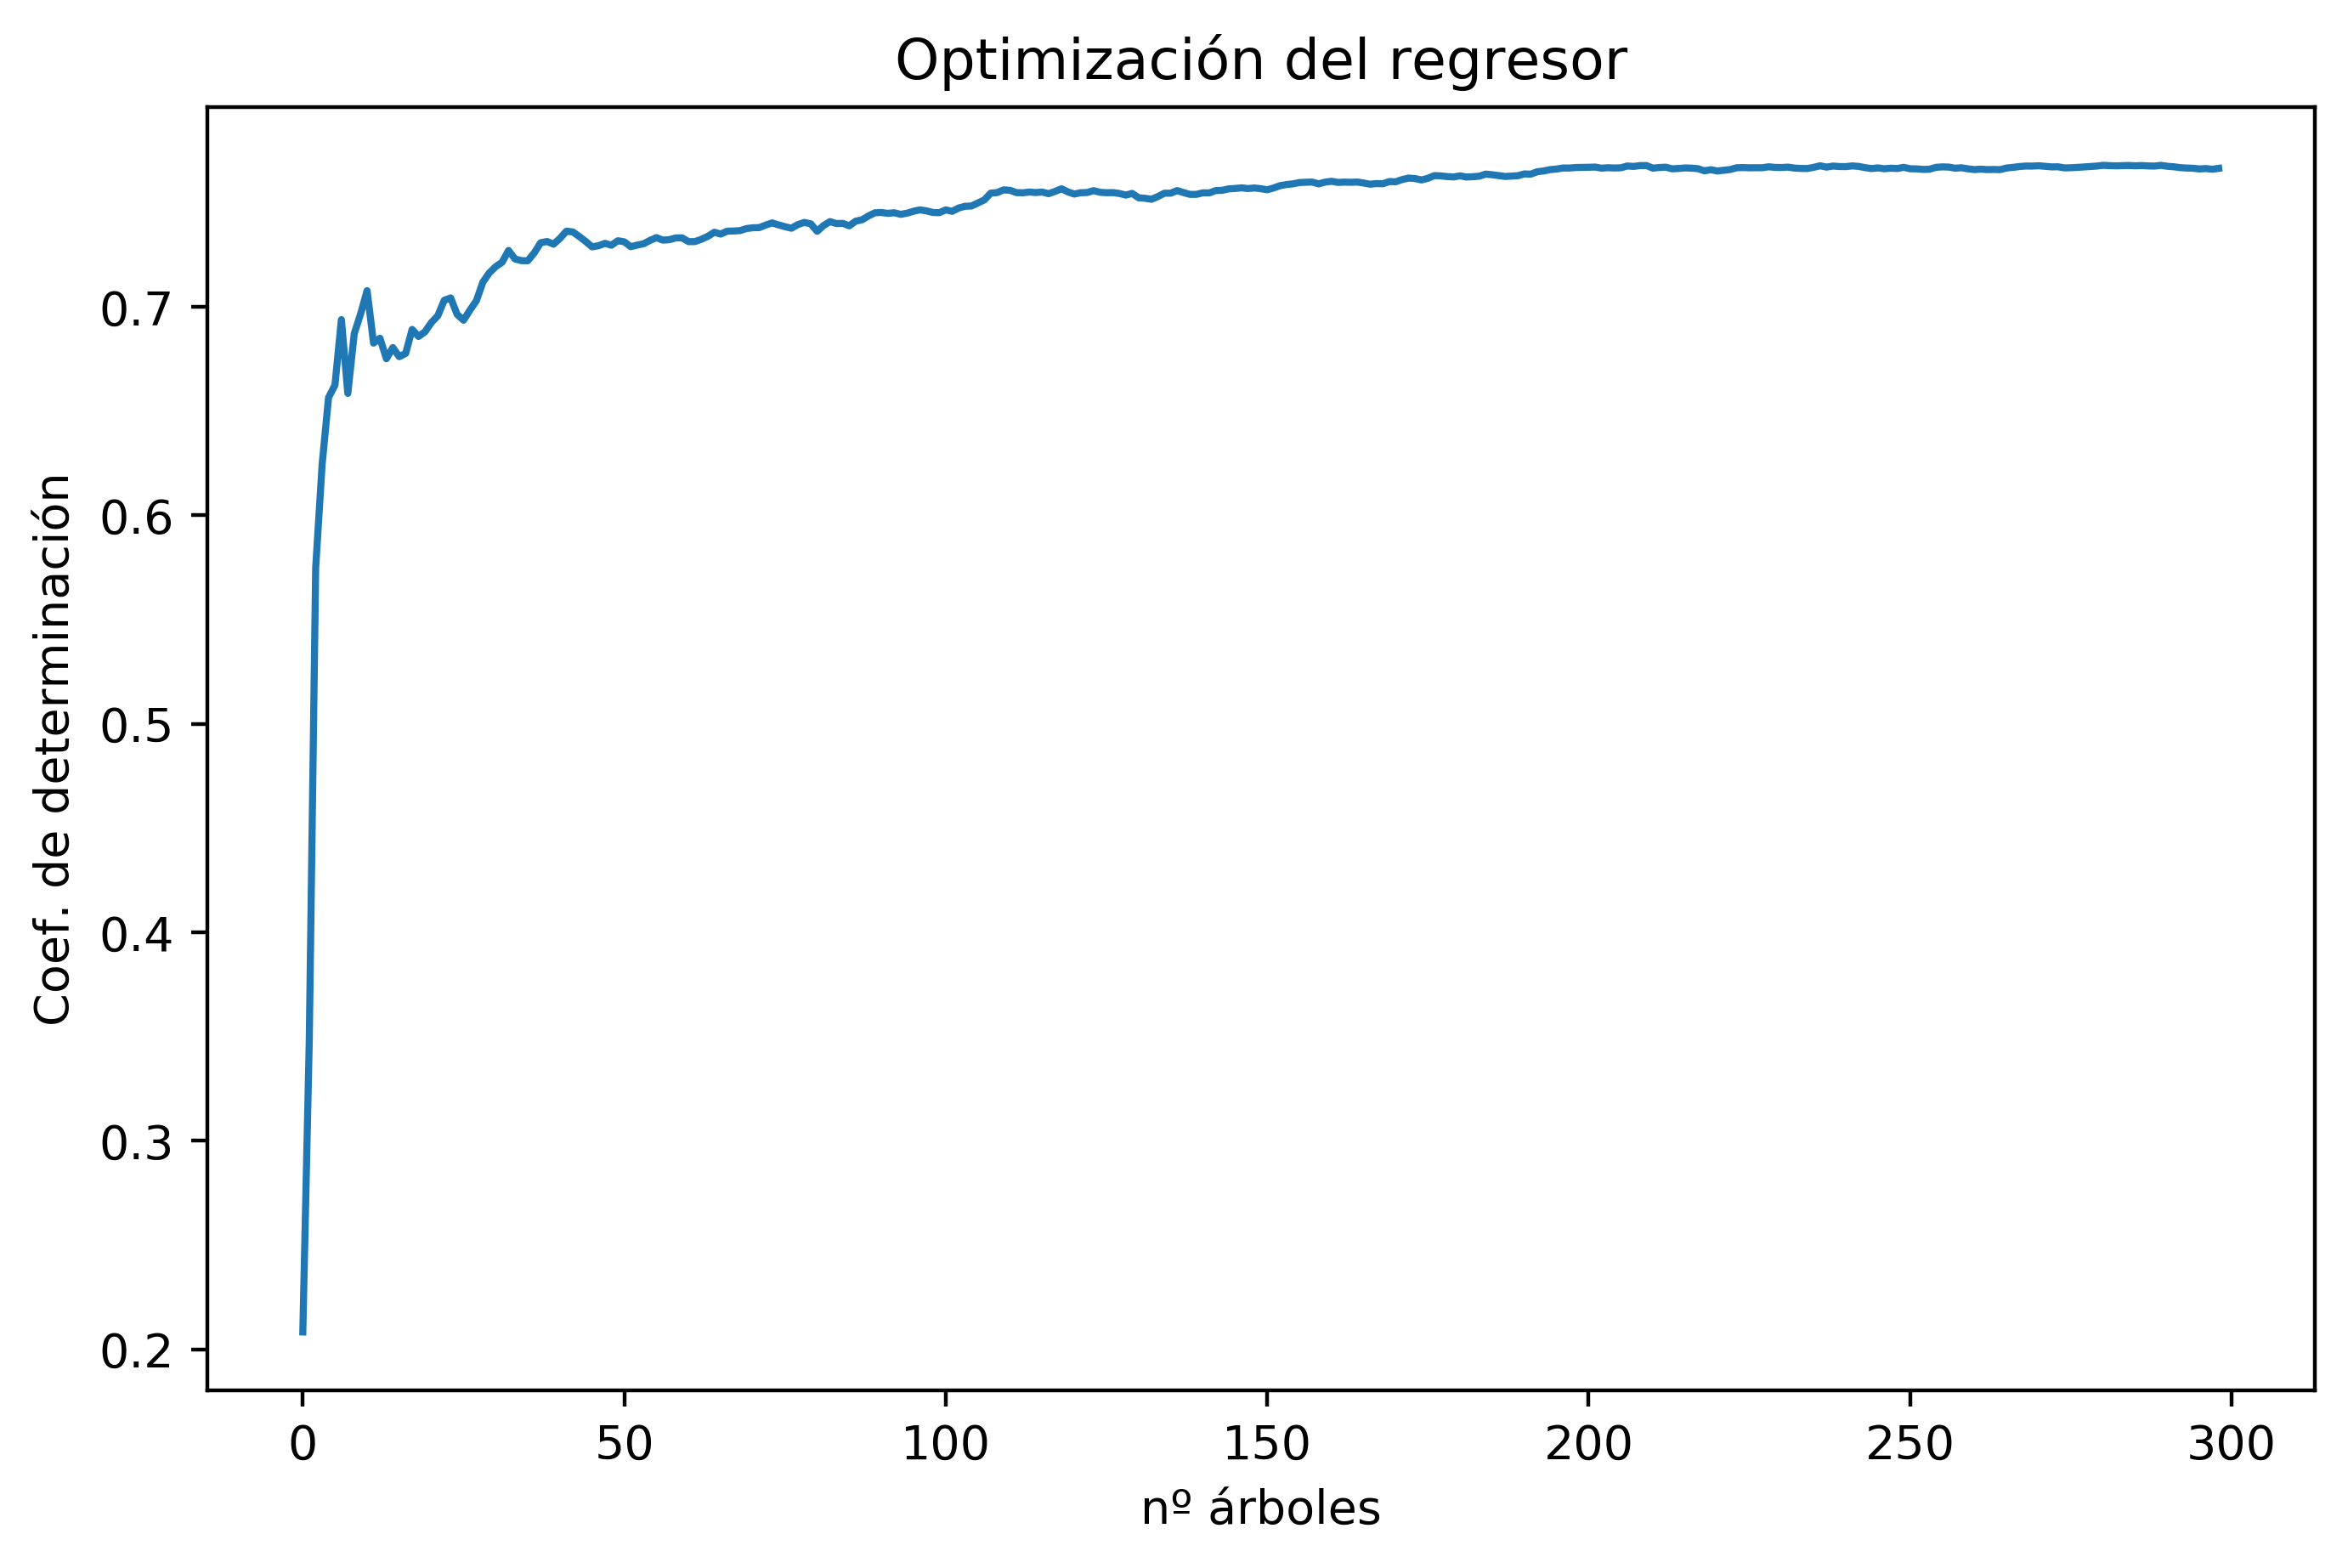
\includegraphics[height=9cm]{archivos/tfg/Mean/opt_tree_bbch_mean} 
    \caption{Optimización del número de árboles para \gls{rfr} en el modelo de salida \gls{bbch}\label{fig:opt_parcl}}
    
\end{figure}

\par Finalmente, los parámetros utilizados en este método para cada caso se presentan en la tabla \ref{tab:opt_parcl}, donde se pueden ver: la parcela utilizada para el periodo de test del modelo; siendo el resto de parcelas utilizadas en el entrenamiento, y el número de árboles óptimo para \gls{rfr}, de acuerdo con la evolución del coeficiente de determinación para cada caso.

\begin{table}[h]
\centering
\begin{tabular}{l|ccc}
                  & \gls{bbch}     & Altura   & \gls{bbch}\&Altura \\ \hline
Parcela de test   & `Mínima' & `Puntal' & `Mínima'     \\
Número de árboles & 42       & 77       & 54          
\end{tabular}
\caption{Parámetros de optimización de entrada y modelo
\label{tab:opt_parcl}}
\end{table}

\par Como se puede observar, los 3 casos de este método constan de un número óptimo de árboles de, al menos, el mismo orden. Cabe destacar que el aumento de complejidad en el modelo y diferente parcela de test en el caso de la altura como salida del sistema. Probablemente se debe a la diferente adaptación a los datos de entrada disponibles, que son distintos a los otros dos casos.  
\subsection{Salidas del modelo}
\subsubsection{Salidas de función de densidad de probabilidad}
Como ya se ha comentado, las salidas del modelo son por defecto predicciones únicas, pero el marco de trabajo anterior demanda salidas en formato \gls{pdf} para ser integradas con el resto del modelo. En las figuras \ref{fig:pdf_b} (modelo de salida \gls{bbch}), \ref{fig:pdf_h} (modelo de salida altura) y \ref{fig:pdf_bh} (modelo de ambas salidas) se puede apreciar cómo son algunas de estas salidas, siendo ejemplos extraídos a partir de los mismos datos para los 3 casos estudiados. 
\\
\par Las \gls{pdf}s se presentan normalizadas con respecto a la salida con mayor probabilidad. En estos ejemplos se puede ver como, aunque hay una salida que predomina con respecto al resto, no se excluyen las demás soluciones posibles. Esto facilita la integración con el modelo de predicción temporal ya que se pueden combinar ambas \gls{pdf} de salida para ver dónde coinciden y con qué probabilidad. En general, los resultados de la predicción temporal son bastante certeros, con oportunidad de fallo para ajustes finos en cultivos que hayan podido sufrir retrasos o adelantos en su desarrollo típico. Es ahí donde la contribución de este modelo es importante, aportando información extra en tiempo real y creando una predicción de cuáles serían los posibles estados de desarrollo en los que se encuentra el cultivo según la información actual de satélite. 
\\
% Una figura con dos imágenes
\begin{figure}[H]
\centering
\begin{subfigure}{0.6\textwidth}
  \centering
  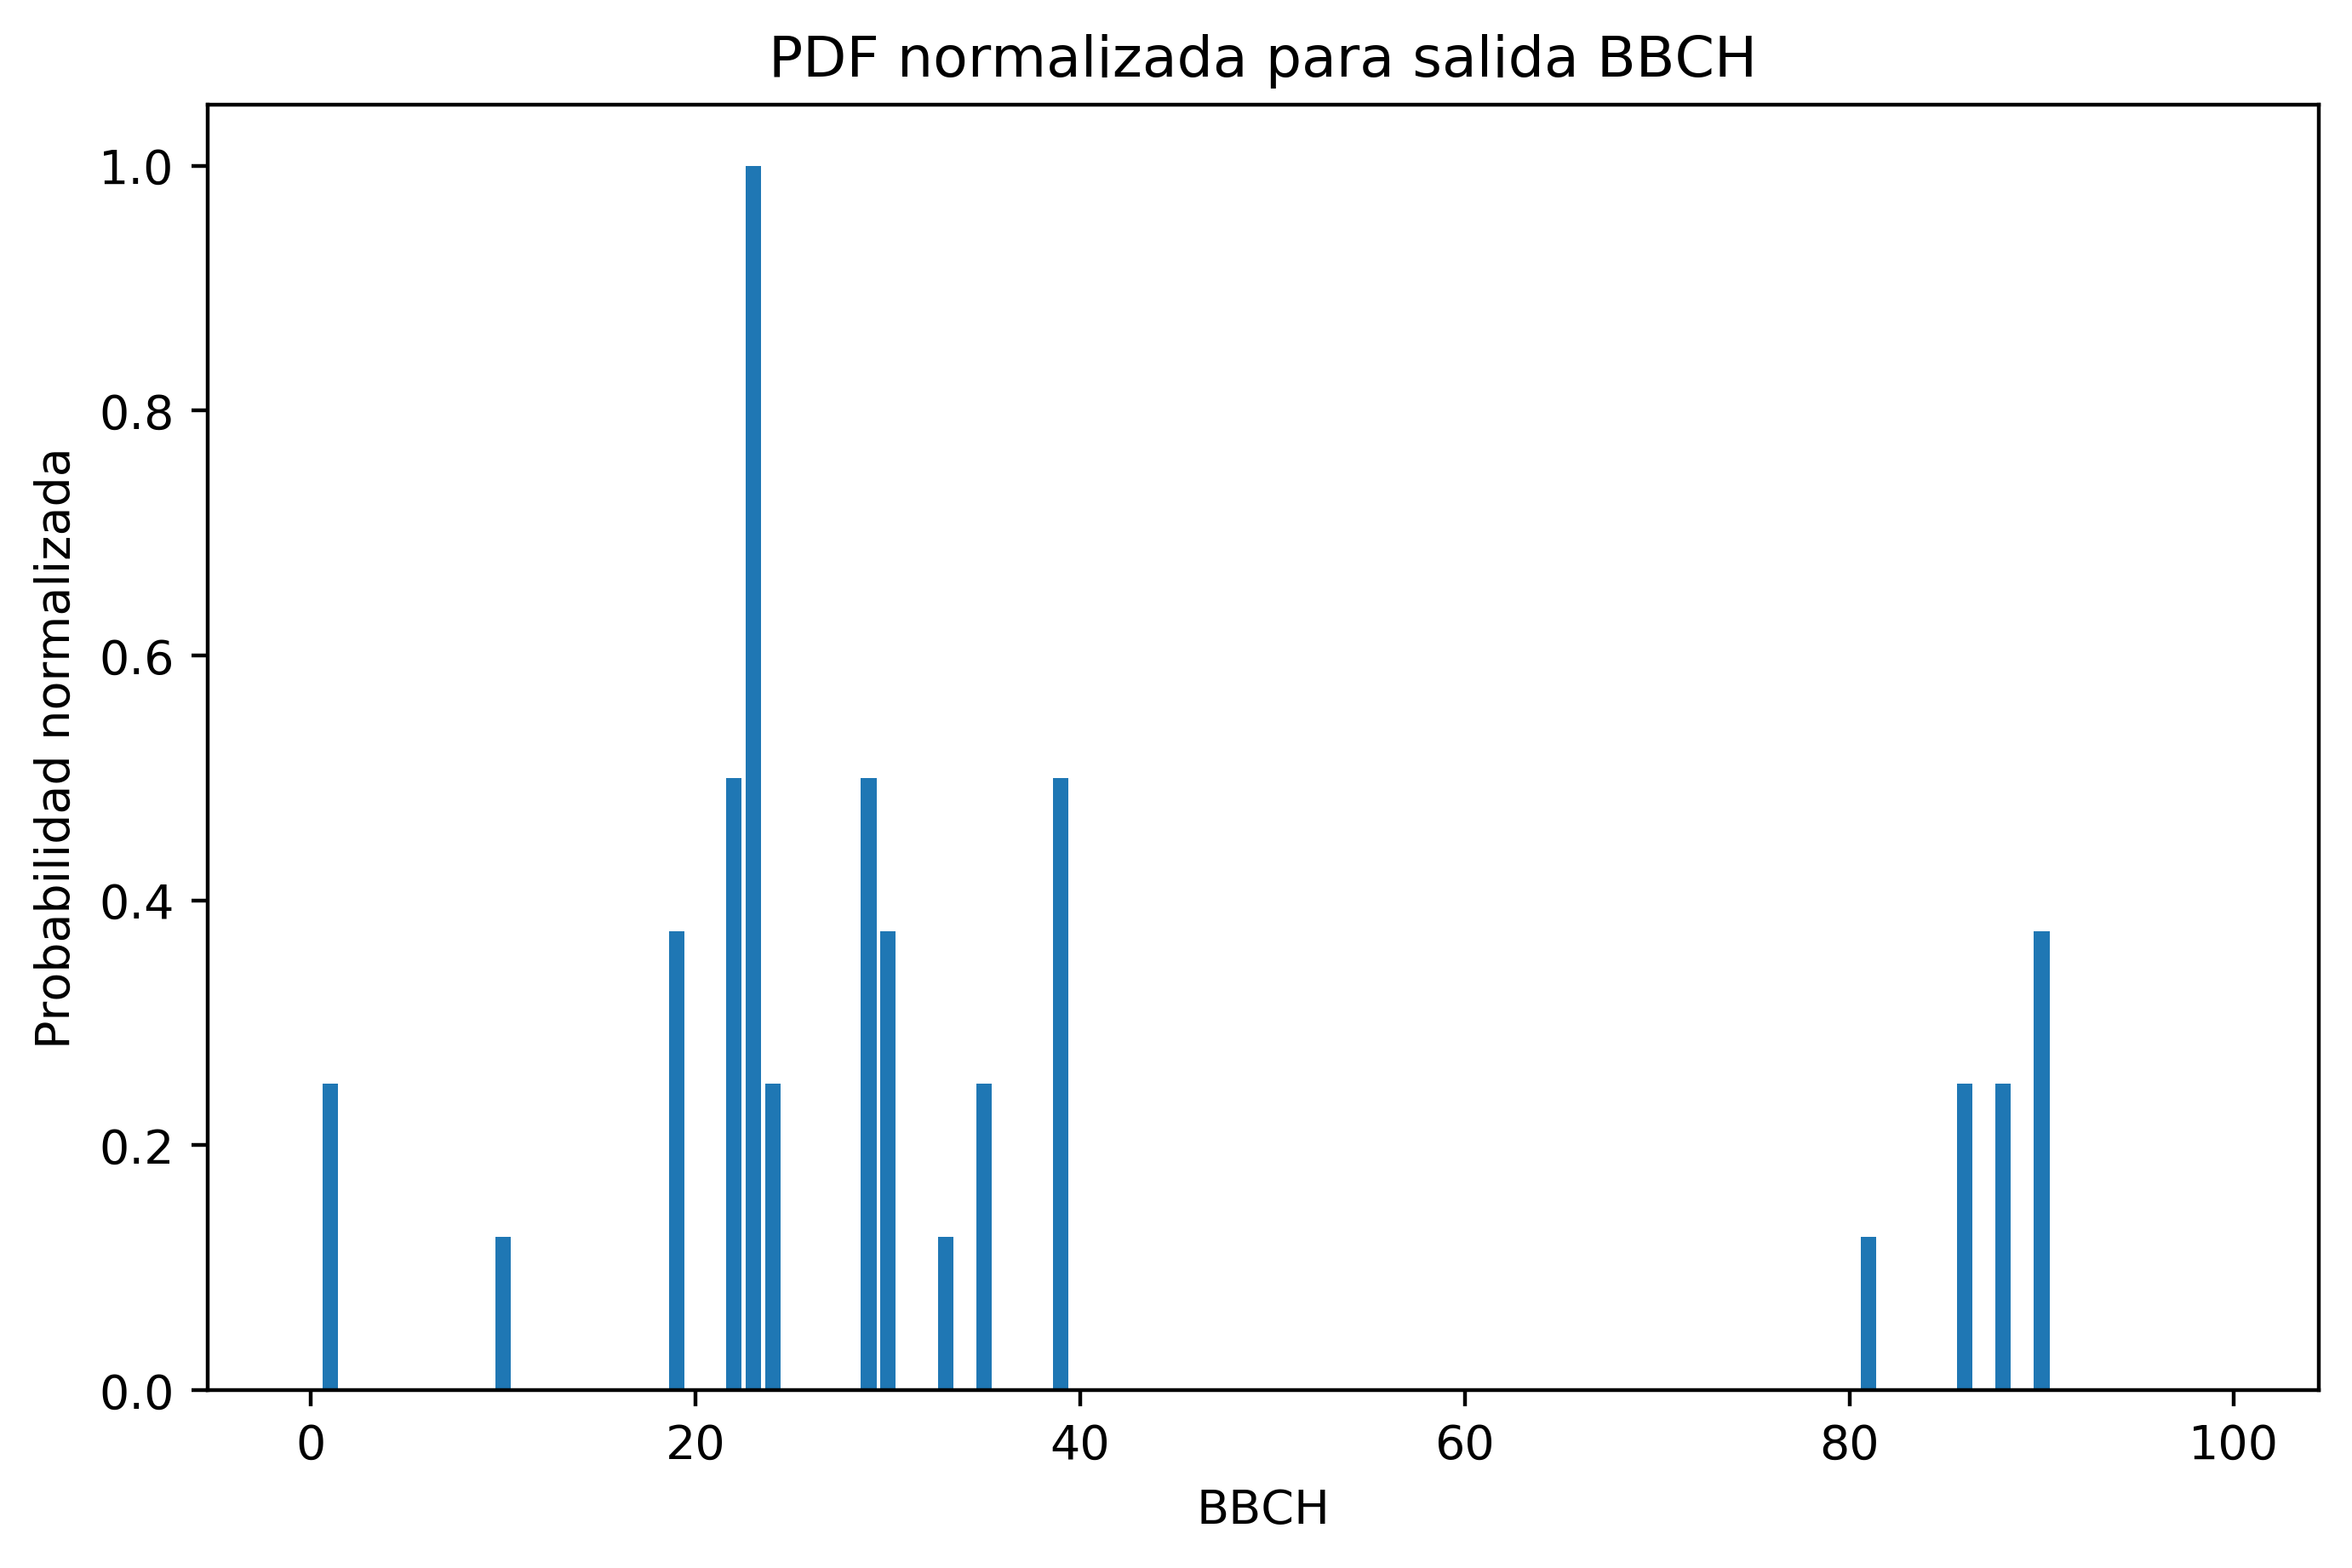
\includegraphics[width=0.95\linewidth]{archivos/tfg/Mean/TEST_PARC_PDF}
  \caption{Ejemplo del modelo de doble salida: \gls{pdf} estimación de \gls{bbch}\label{fig:pdf_b}}
\end{subfigure}
\begin{subfigure}{0.6\textwidth}
  \centering
  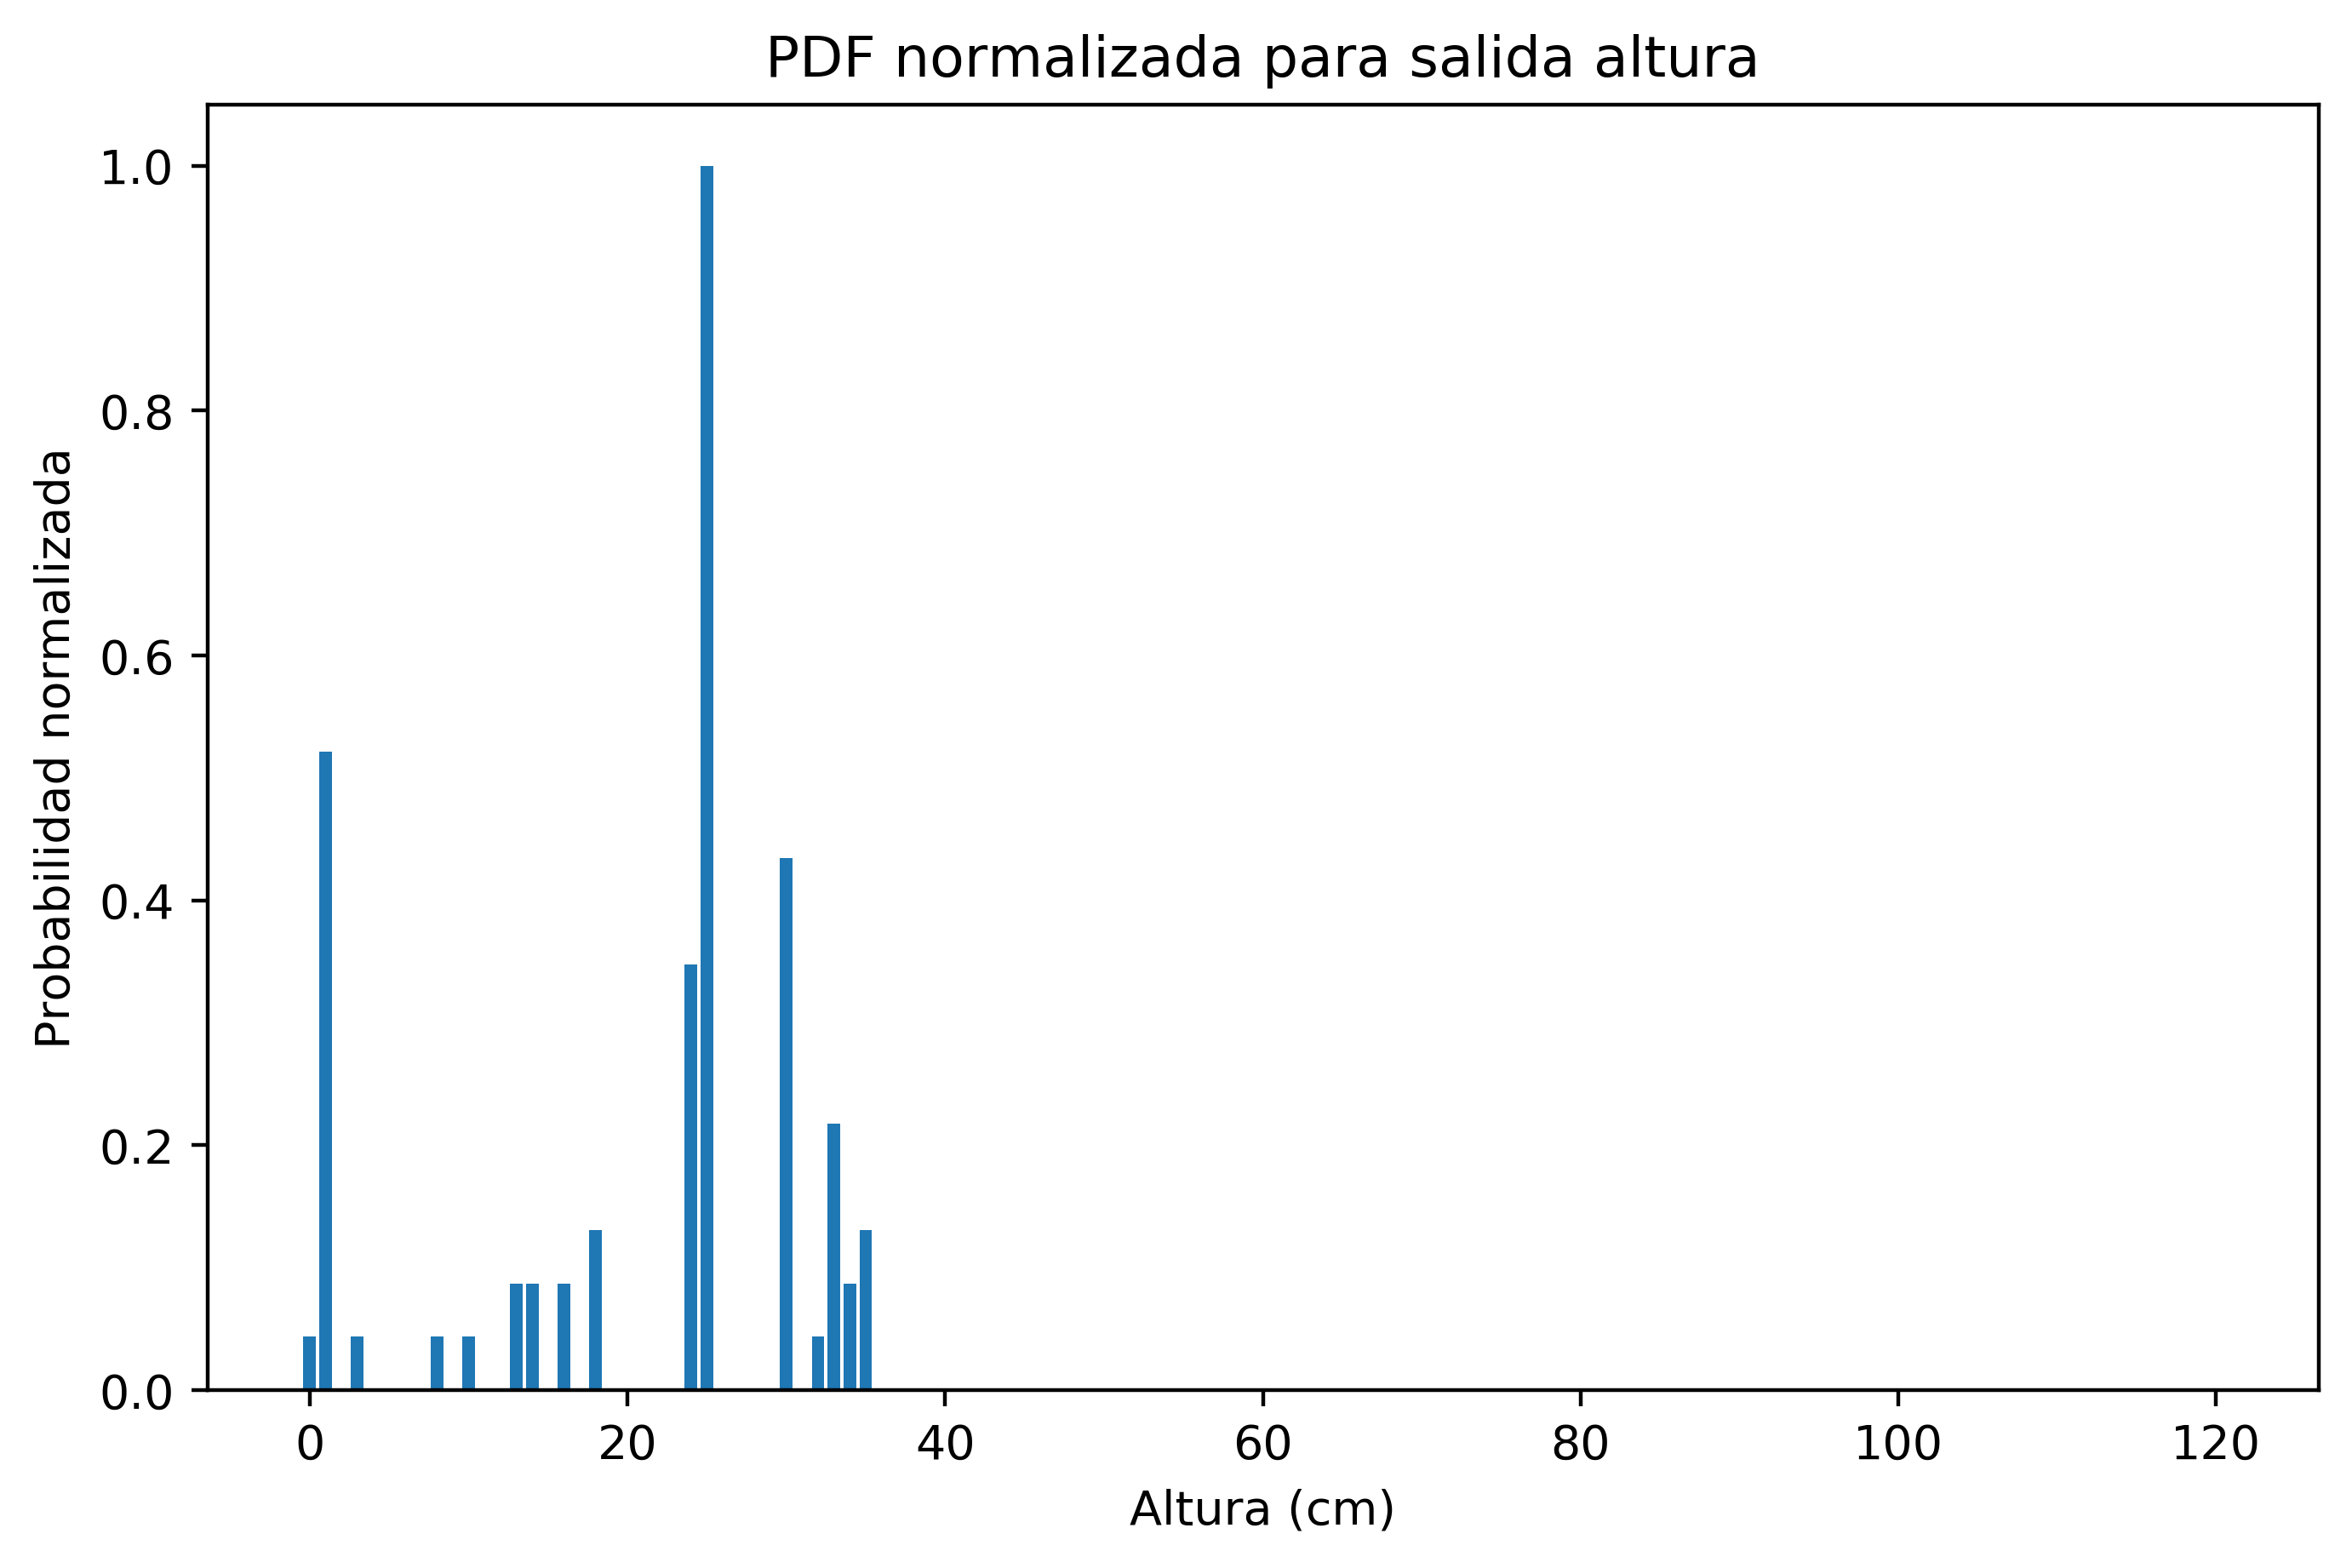
\includegraphics[width=0.95\linewidth]{archivos/tfg/Mean/TEST_PARC_PDF_H}
  \caption{Ejemplo del modelo de doble salida: \gls{pdf} estimación de altura\label{fig:pdf_h}}
\end{subfigure}
\caption{Ejemplo de salidas \gls{pdf} normalizadas del modelo para estimación de \gls{bbch} y la altura. \label{fig:pdf_bh}}
\end{figure}
\par Las 3 figuras \ref{fig:pdf_b}, \ref{fig:pdf_h} y \ref{fig:pdf_bh} han sido generadas con los mismos datos de entrada, es decir, los mismos datos de satélite en la misma parcela y fecha, por lo que las salidas para los modelos generados de estimación de \gls{bbch} (Figura \ref{fig:pdf_b}) y altura (Figura \ref{fig:pdf_h}) como modelos independientes se pueden comparar con las salidas del modelo de estimación de ambas (Figura \ref{fig:pdf_bh}). La principal diferencia que encontramos entre los mismos tipos de datos de salida para cada modelo es que, en general, las salidas individuales presentan una estimación principal con una diferencia de probabilidad mucho mayor con respecto al resto que las estimaciones del modelo de doble salida. El rango para cada salida se mantiene bastante similar en ambos modelos, además del valor con la probabilidad más alta, aunque la disminución de diferencias con las demás estimaciones, sobre todo en el caso de la altura (\ref{fig:sub2}), indica que ese sistema es menos preciso y estable. El hecho de que sea la salida de la altura la que se vea más perjudicada en este modelo de dos salidas puede deberse a que la optimización de este, en cuanto a número de árboles del regresor, es más similar, y por lo tanto más beneficiosa, con respecto al caso individual de estimación de \gls{bbch}.

% Una figura con dos imágenes
\begin{figure}[H]
\centering
\begin{subfigure}{0.6\textwidth}
  \centering
  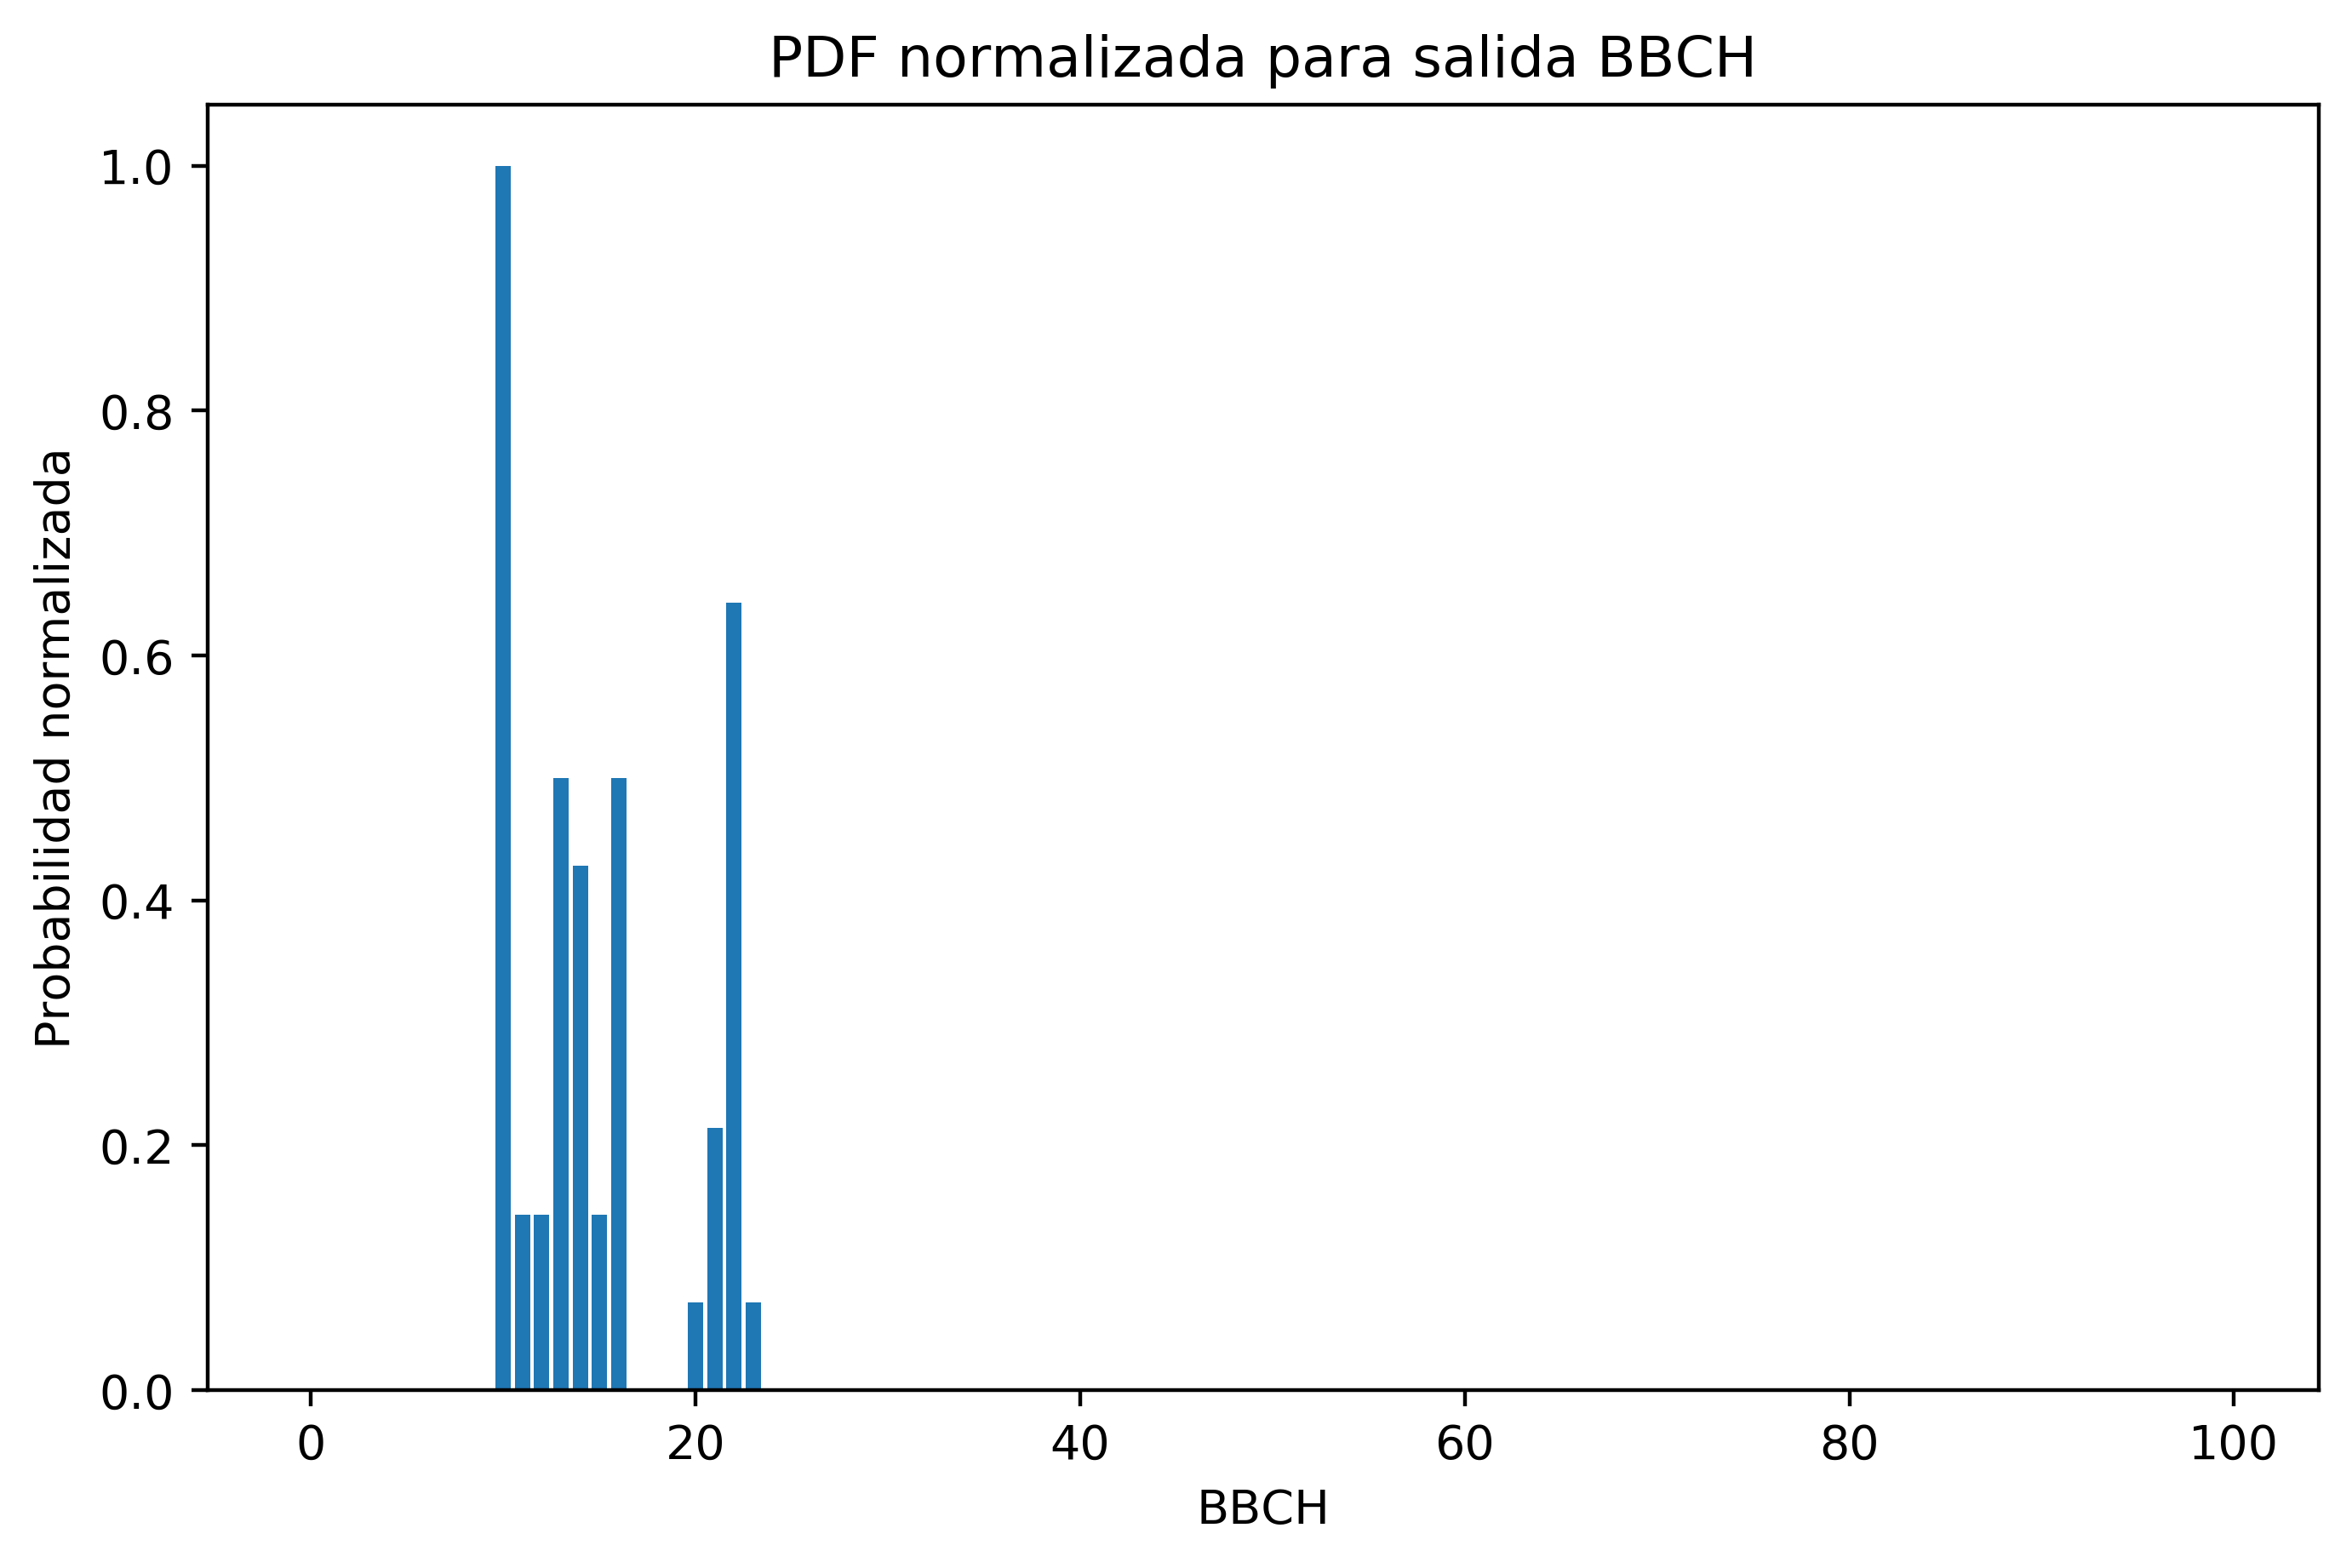
\includegraphics[width=0.95\linewidth]{archivos/tfg/Mean/TEST_PARC_PDF_BH_B}
  \caption{Ejemplo del modelo de doble salida: \gls{pdf} estimación de \gls{bbch}\label{fig:sub1}}
\end{subfigure}
\begin{subfigure}{0.6\textwidth}
  \centering
  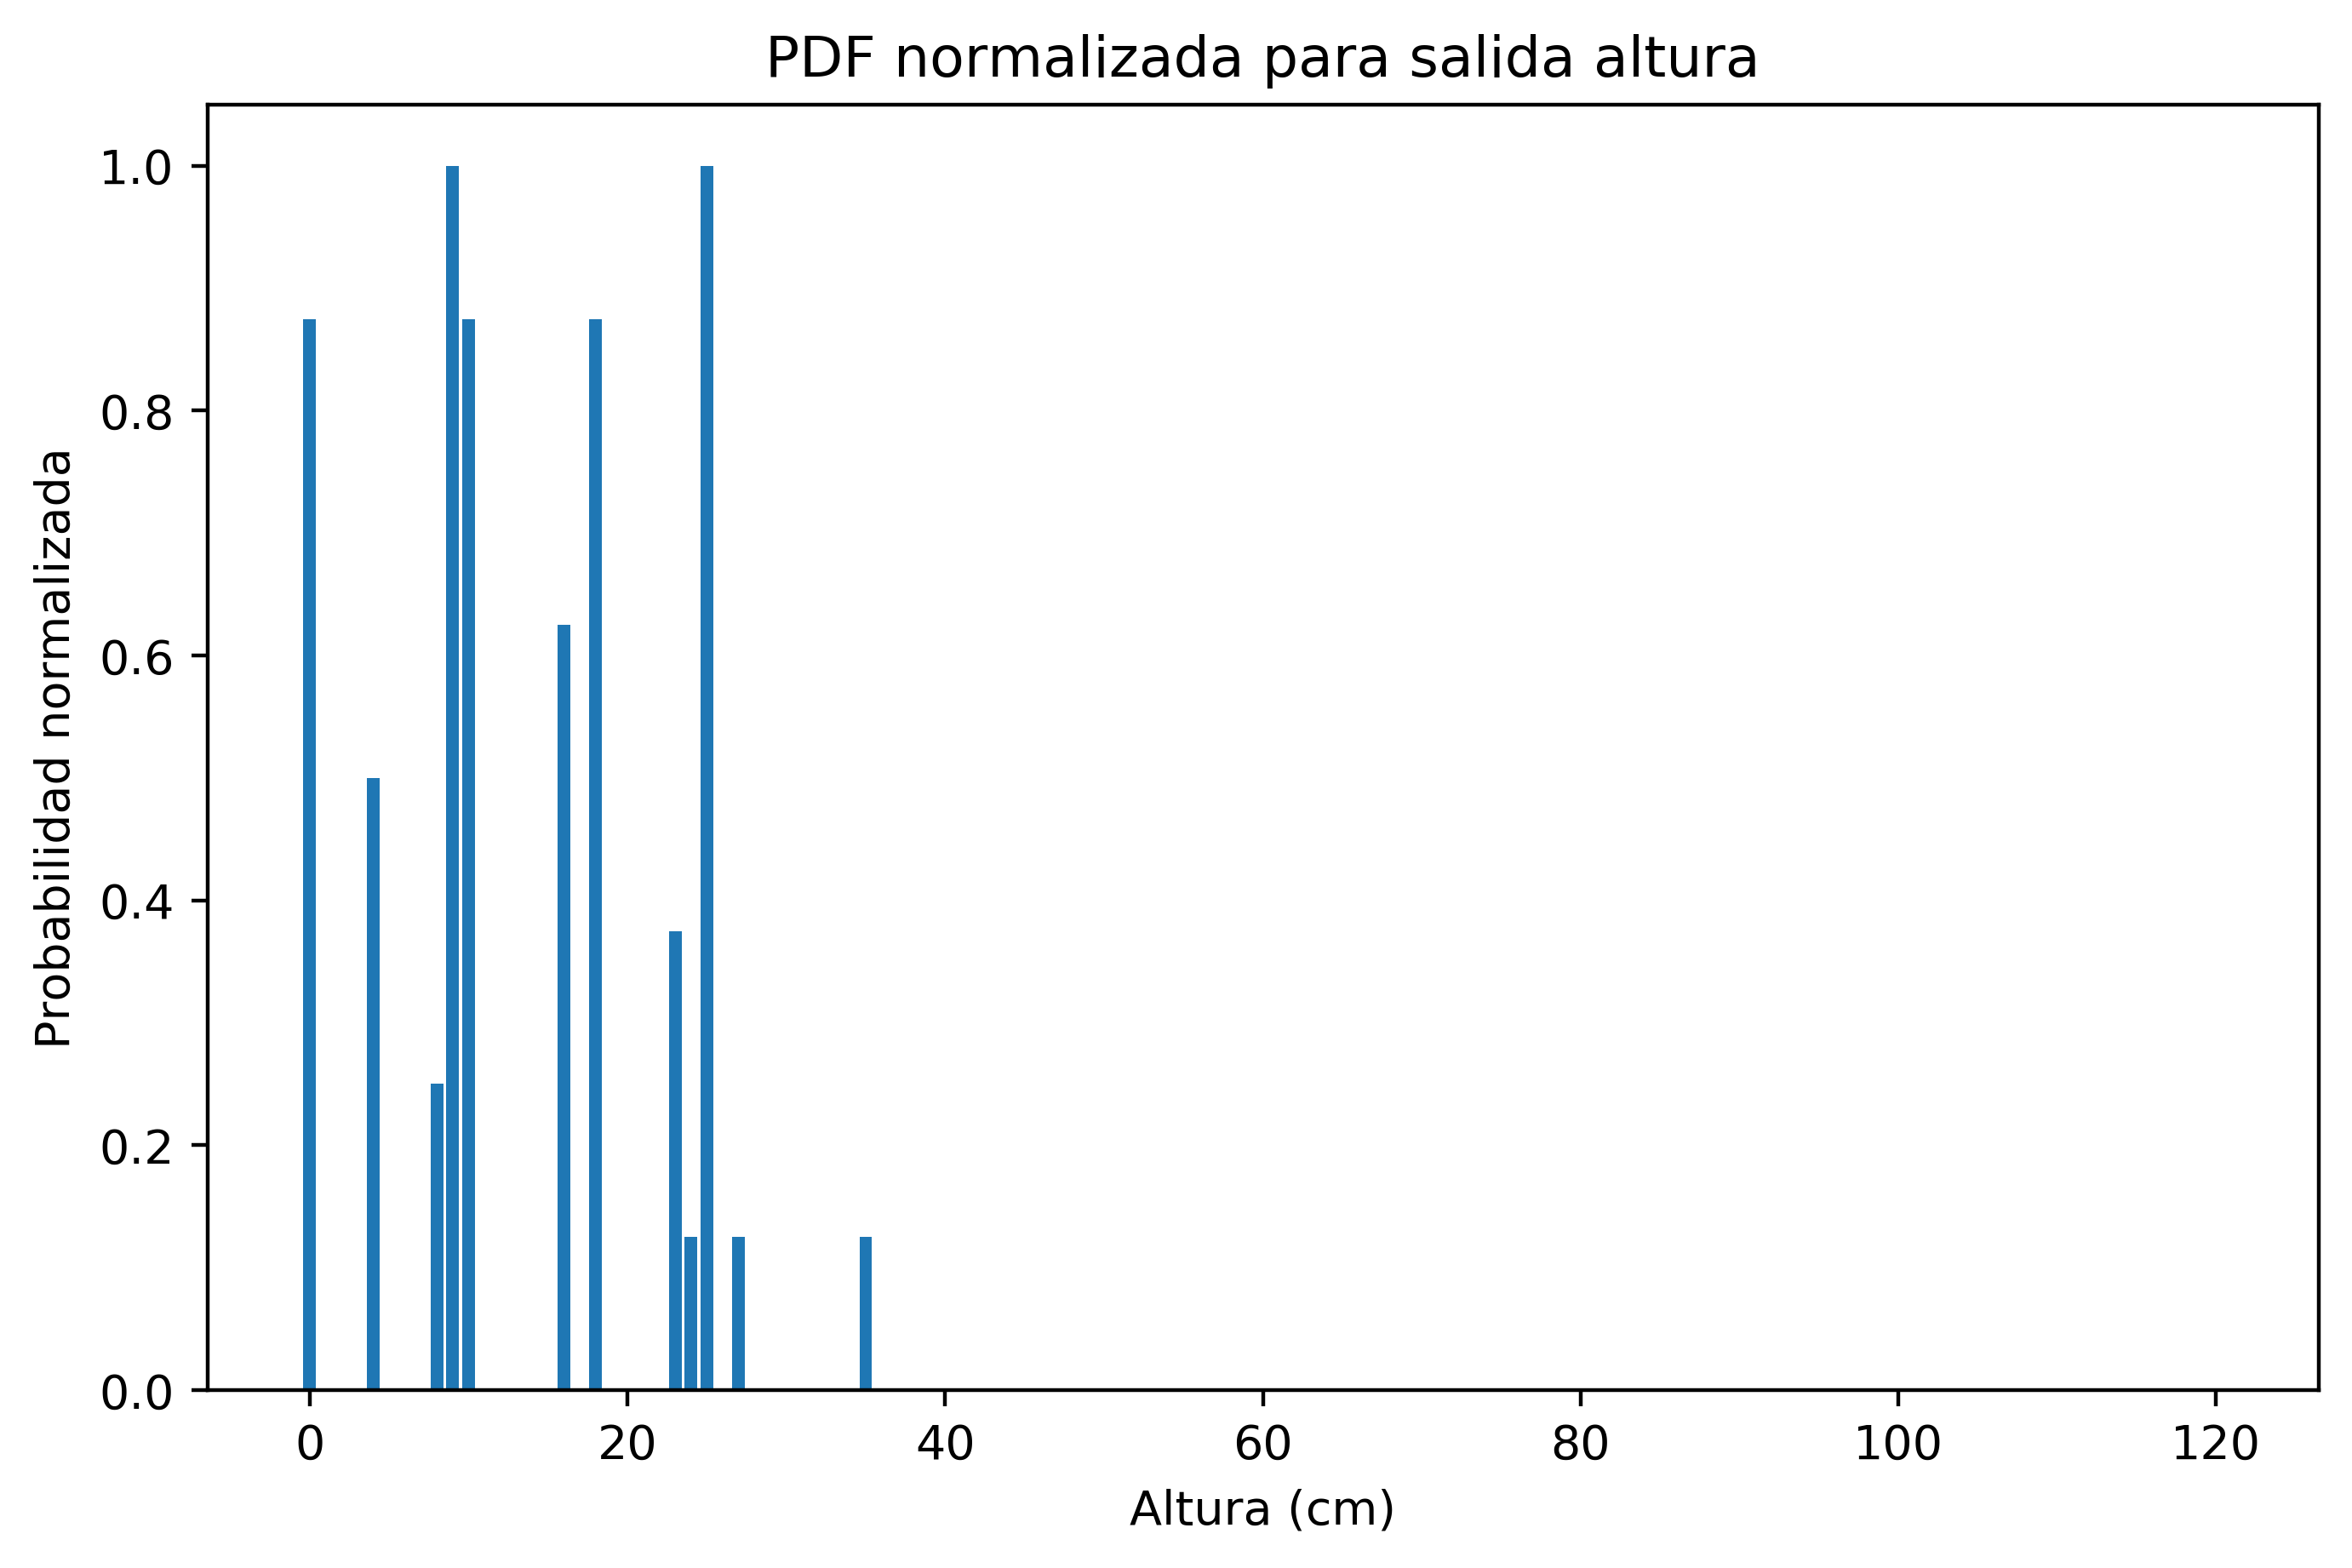
\includegraphics[width=0.95\linewidth]{archivos/tfg/Mean/TEST_PARC_PDF_BH_H}
  \caption{Ejemplo del modelo de doble salida: \gls{pdf} estimación de altura\label{fig:sub2}}
\end{subfigure}
\caption{Ejemplo de salidas \gls{pdf} normalizadas del modelo para estimación de \gls{bbch} y la altura. \label{fig:pdf_bh}}
\end{figure}

\subsubsection{Salidas de valor único}
\par Para continuar con la presentación de los resultados obtenidos, se ilustran en las figuras \ref{fig:comp_b}, \ref{fig:comp_h} y \ref{fig:comp_bh} las comparaciones de las soluciones únicas obtenidas (salida con máxima probabilidad) y los datos de tierra tomados correspondientes para la parcela de test en 2018: \gls{bbch} general, máxima y mínima en la parcela, casos individual (\ref{fig:comp_b}) y de doble salida (\ref{fig:sub_c1}), o la altura general del cultivo, también para ambos casos (figuras \ref{fig:comp_h} y \ref{fig:sub_c2}, respectivamente). Estas salidas, aunque carecen de la información completa, son las más sencillas de comparar y evaluar con los resultados reales, ya que estos también son un único valor.  
\\

% Dos figuras sueltas debajo de otra
\begin{figure}[H]
\centering
\begin{subfigure}{.65\textwidth}
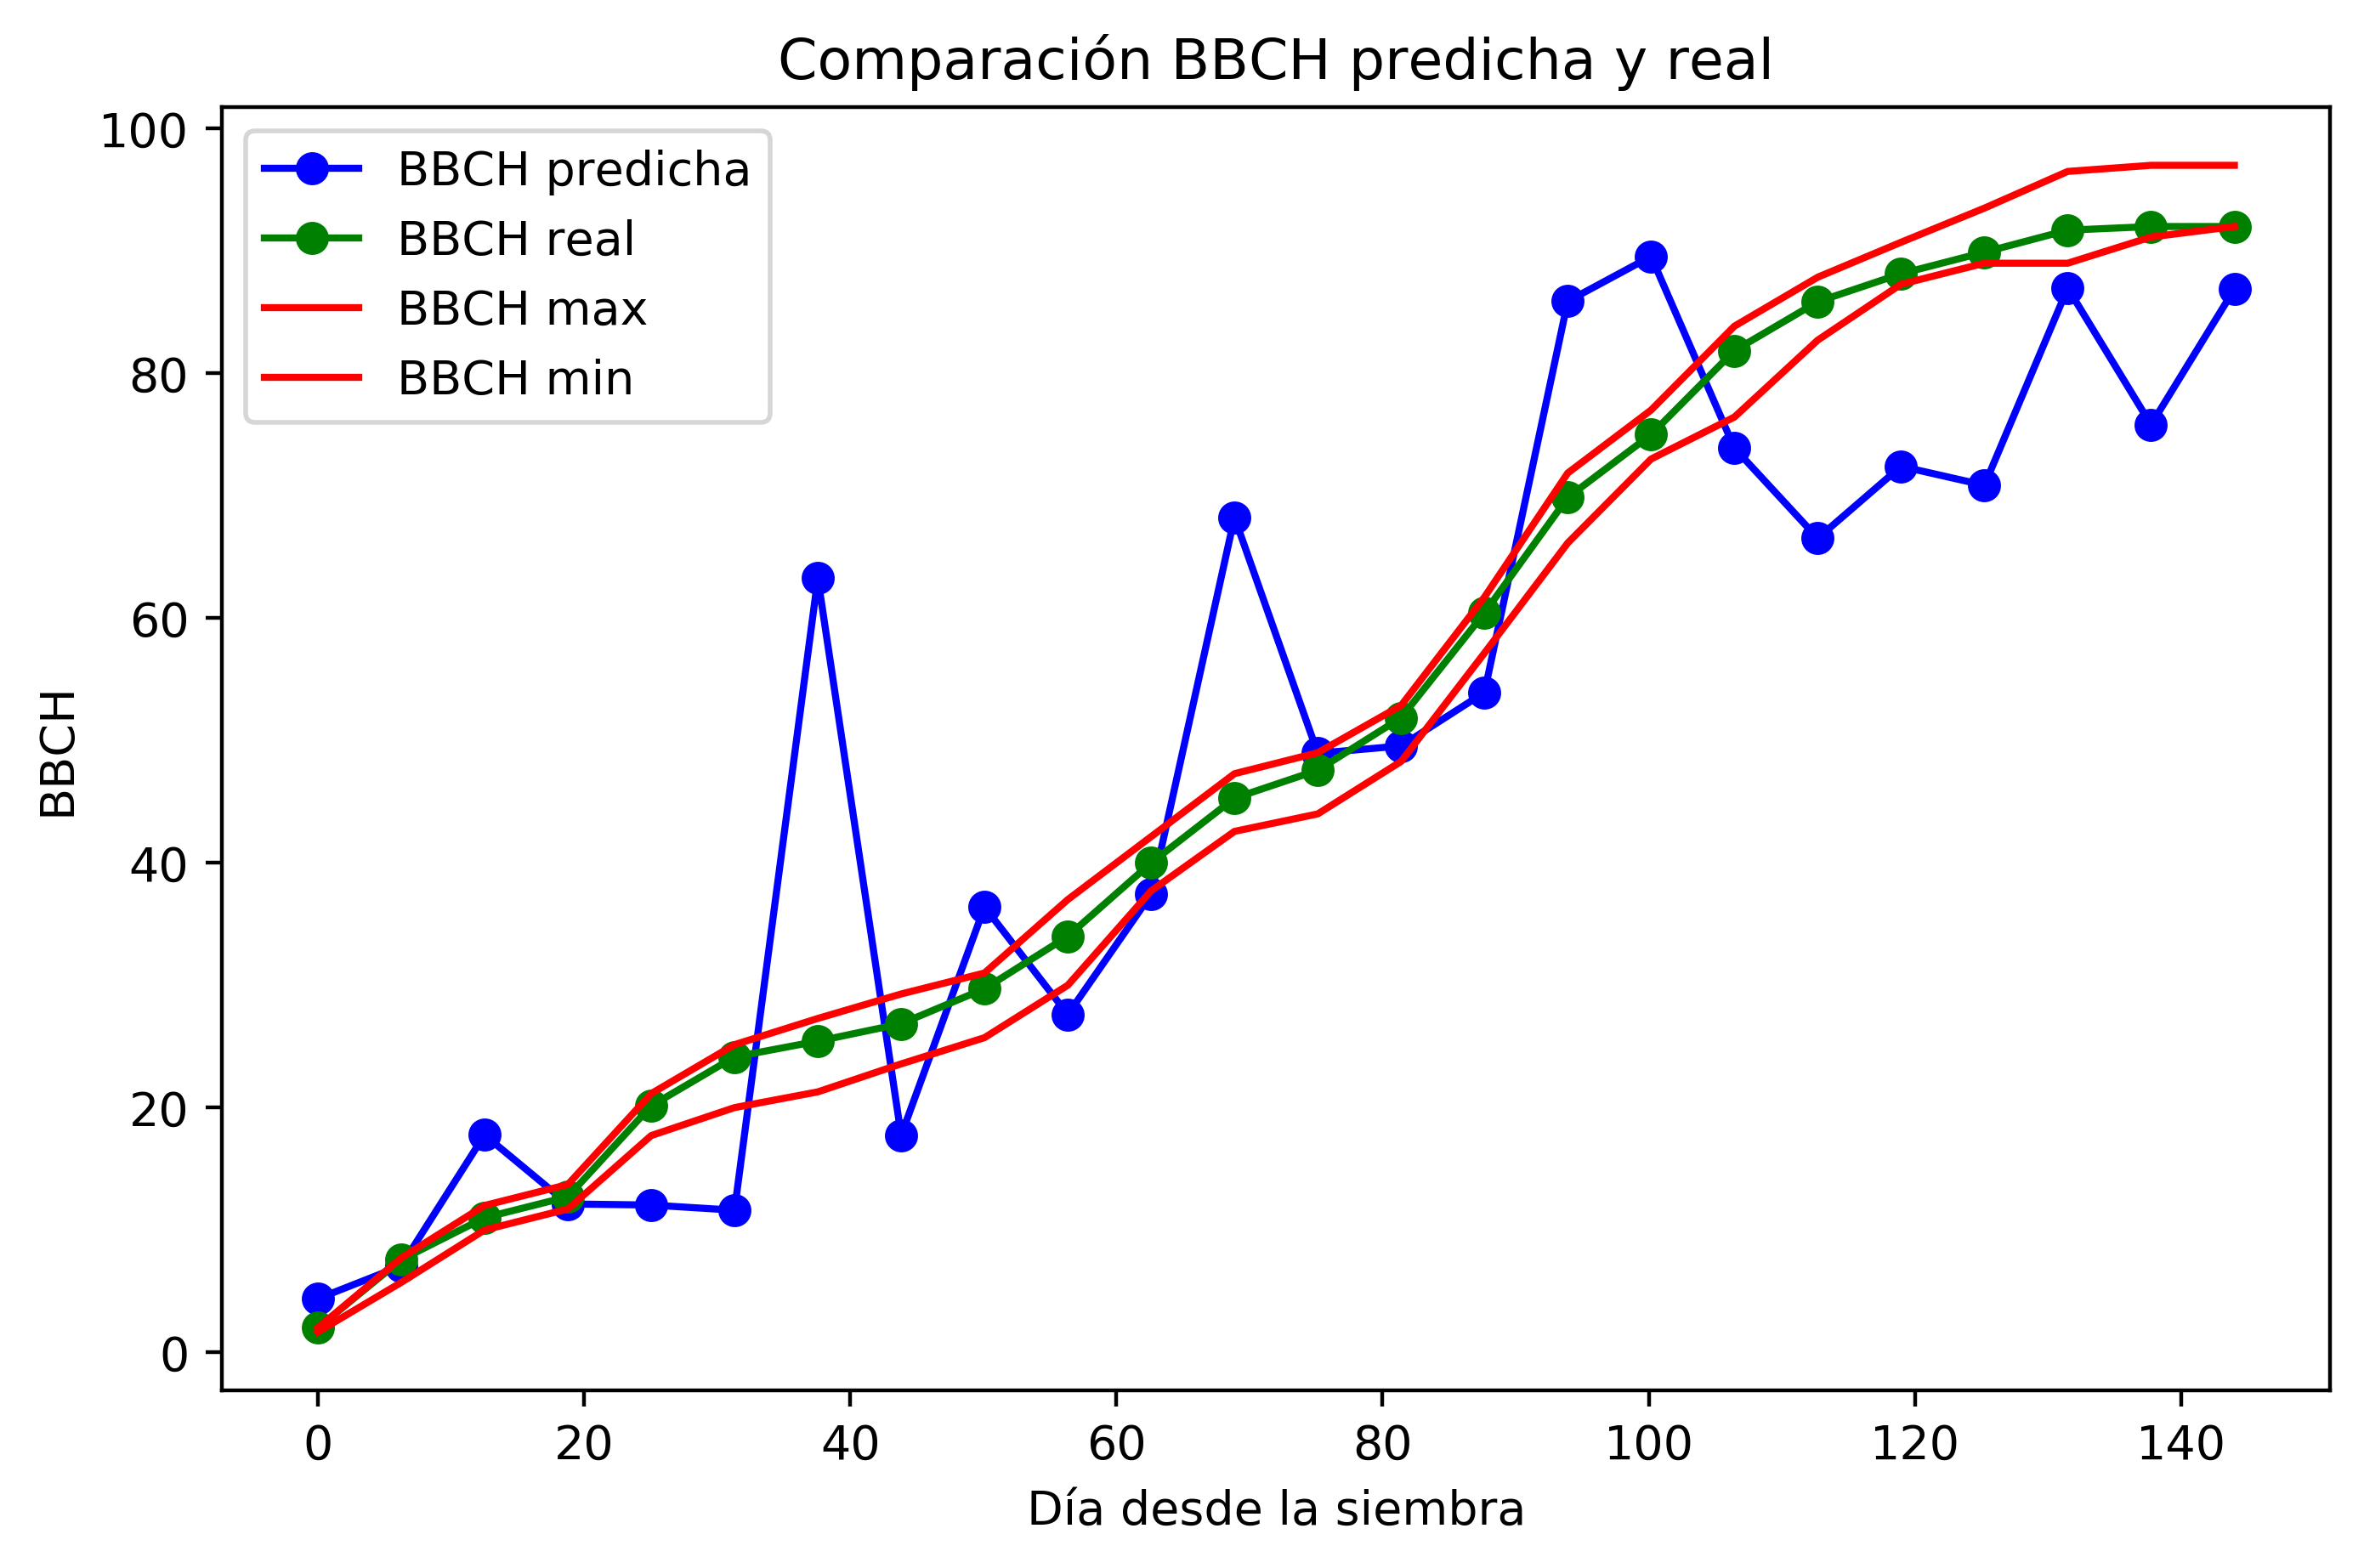
\includegraphics[width=0.95\linewidth]{archivos/tfg/Mean/TEST_PARC_FINAL}
\captionof{figure}{Comparación de la salida predicha y la verdad de tierra del modelo para estimación de \gls{bbch}.\label{fig:comp_b}}
\end{subfigure}
\begin{subfigure}{.65\textwidth}
\centering
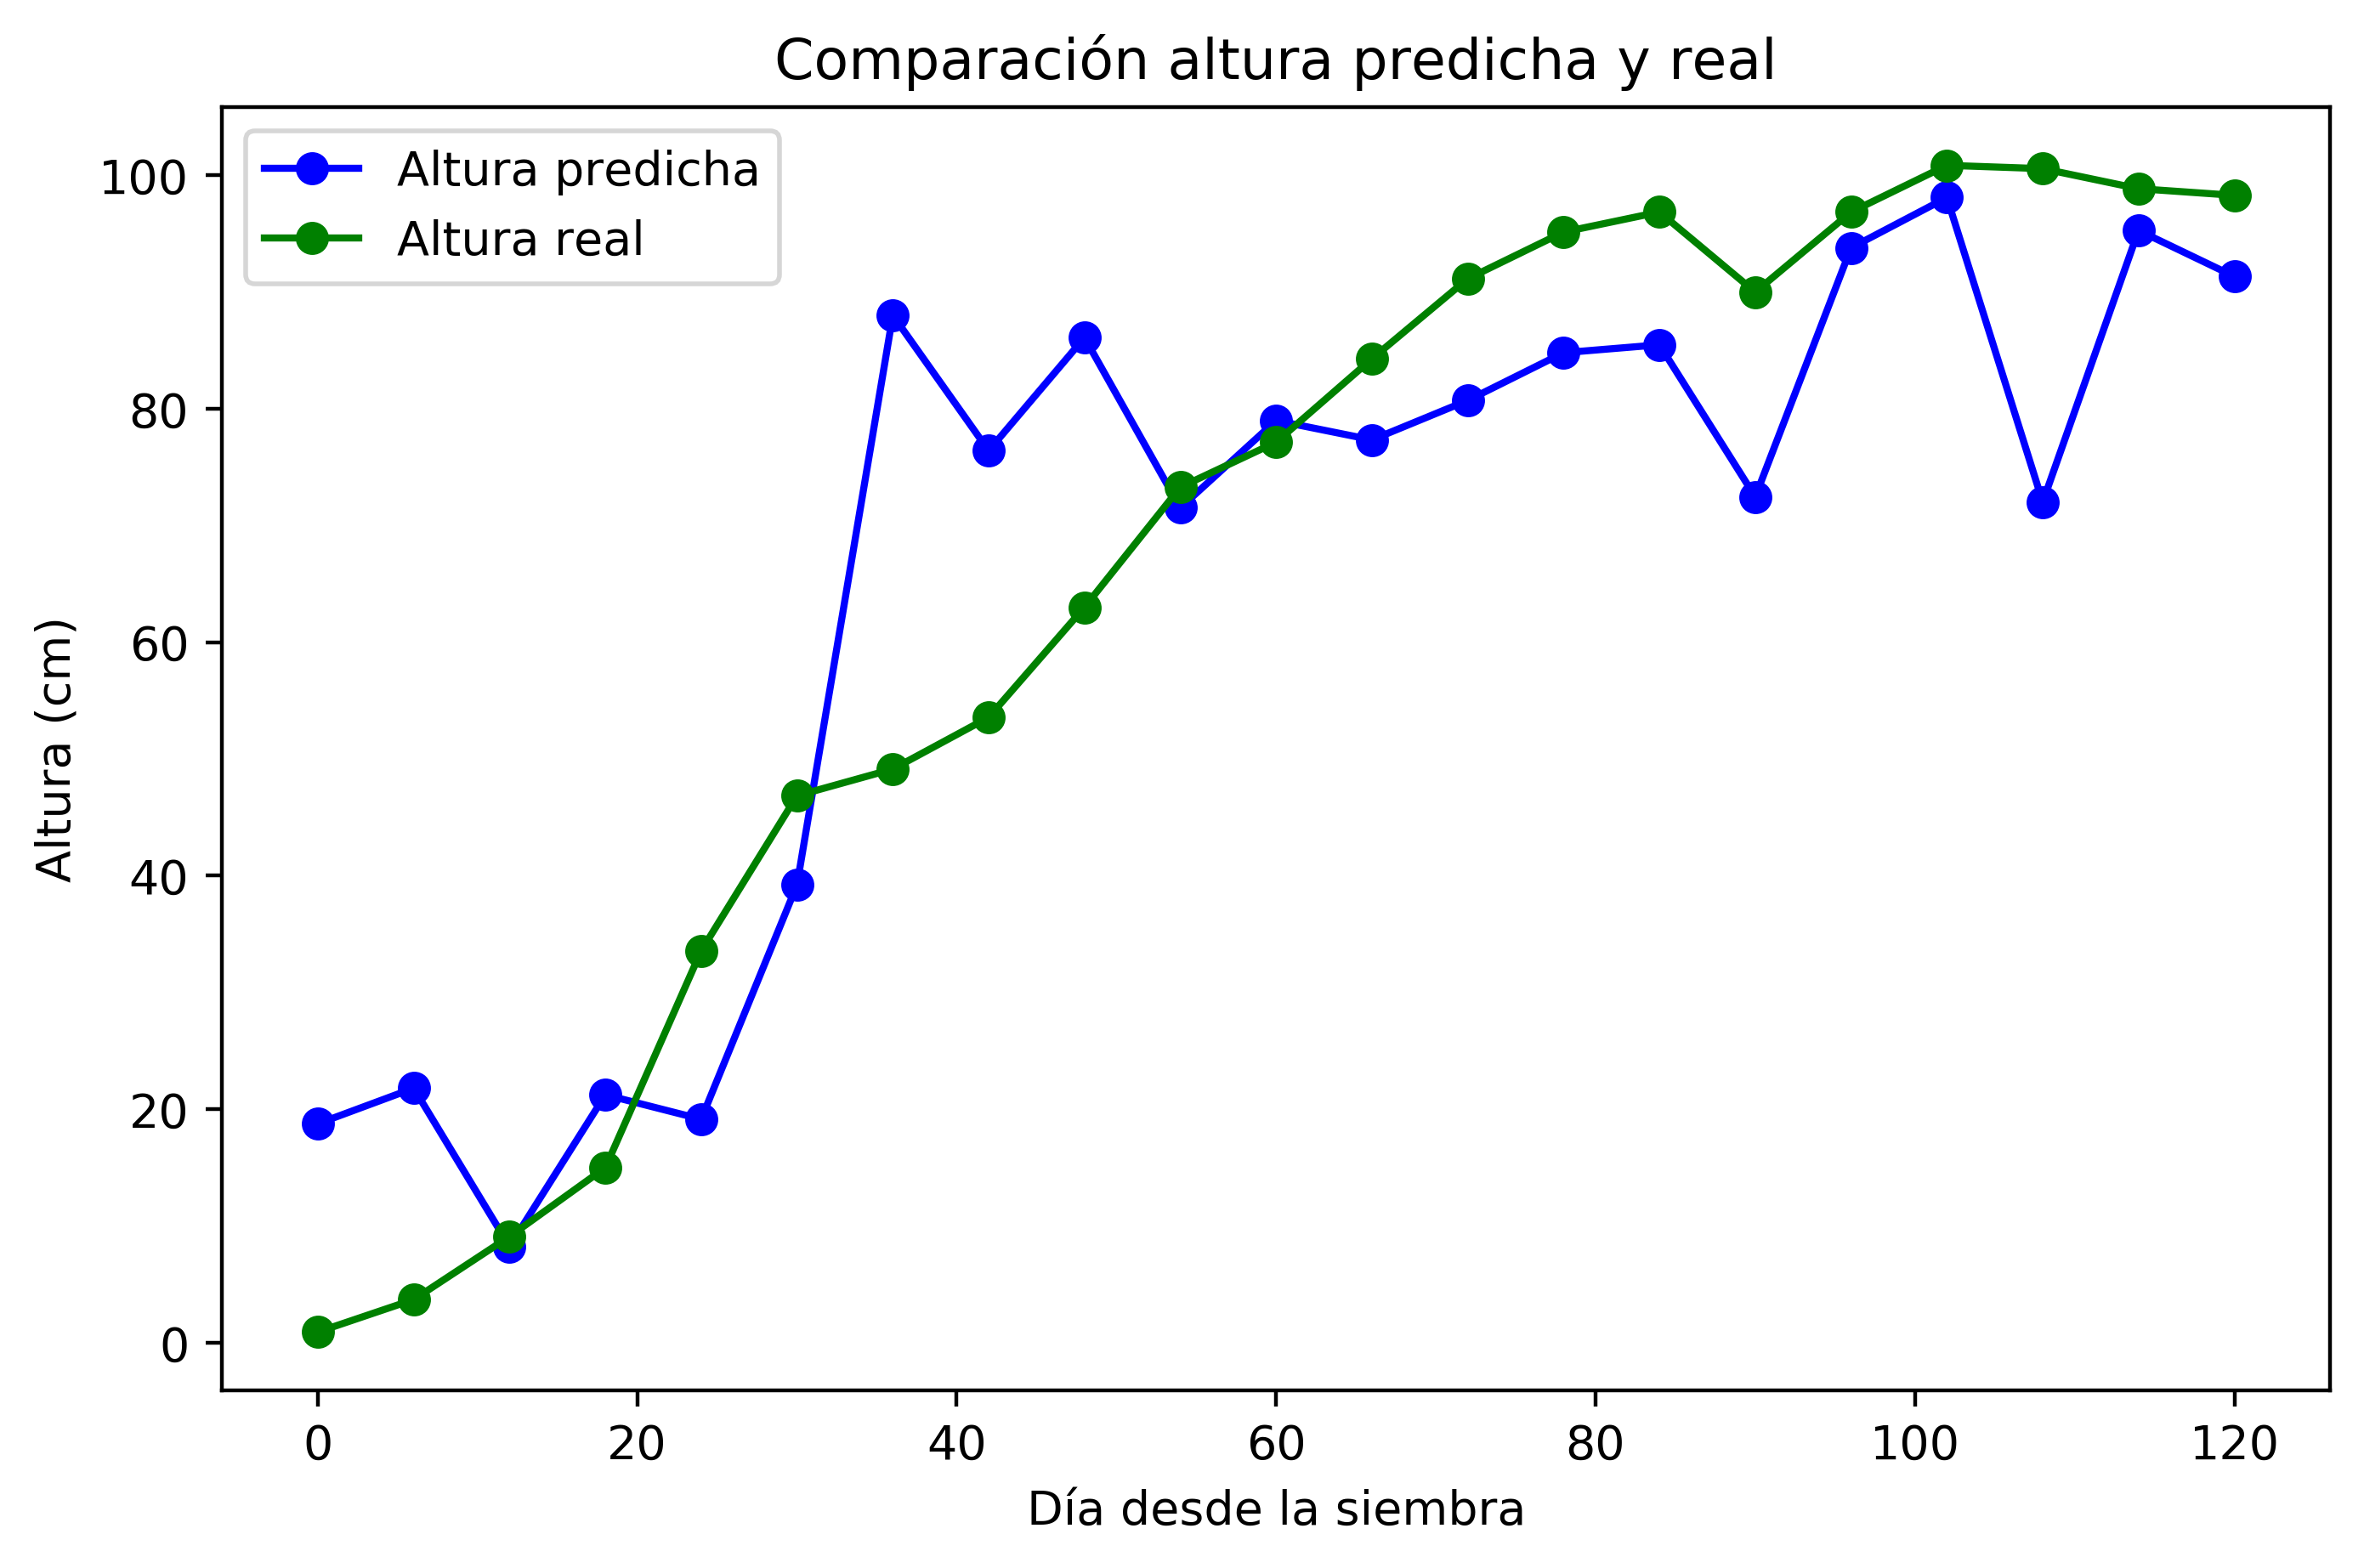
\includegraphics[width=0.95\linewidth]{archivos/tfg/Mean/TEST_PARC_FINAL_H}
\captionof{figure}{Comparación de la salida predicha y la verdad de tierra del modelo para estimación de la altura. \label{fig:comp_h}}
\end{subfigure}
\caption{Comparación de la salida predicha y la verdad de tierra de los modelos de salida individual para la estimación de \gls{bbch} y la altura.}
\end{figure}

\par Comenzando por los modelos de predicción de \gls{bbch} representados en las figuras \ref{fig:comp_b} y \ref{fig:sub_c1}, se pueden observar estimaciones y errores muy parecidos en ambos modelos. Estos son fácilmente comparables ya que la parcela de test coincide para los dos casos. Ambos modelos, presentan estimaciones que, en su mayoría, están fuera de los límites marcados por las líneas de \gls{bbch} máximas y mínimas medidas en campo. En general, se ve una tendencia creciente a lo largo de la variable estimada entorno a los valores reales, aunque con 2 o 3 zonas con picos de error mayor en las que el sistema predice un estado fenológico mayor al real. De hecho, el primer pico en torno a los días 30-40 después de la siembra está presente tanto en la estimación de \gls{bbch} como de la altura en las figuras \ref{fig:comp_h} y \ref{fig:sub_c2}. Teniendo en cuenta que los valores de entrada son iguales para todos los casos, se puede atribuir este fenómeno a anomalías presentes en los datos de satélite, los cuales, en  una etapa concreta del desarrollo del cultivo, pueden presentar valores muy similares a los obtenidos para etapas finales, y por ello cometer un error de predicción bastante grande. Este error sería corregible bien detectando la anomalía y eliminando o modificando esta parte de los datos de entrada, tanto en entrenamiento como en test o futuros usos, o bien comprobando que el modelo está generando predicciones correctas con menor densidad de probabilidad, estando representadas en las salidas de \gls{pdf}, y pudiendo ser consideradas sin un procesamiento extra de los datos, simplemente al contrastarlos con los resultados del modelo temporal, ya que es una diferencia de etapas muy grande y en este modelo no se daría un error de etapa de tal dimensión. 
\\

% Una figura con dos imágenes
\begin{figure}[H]
\centering
\begin{subfigure}{.65\textwidth}
  \centering
  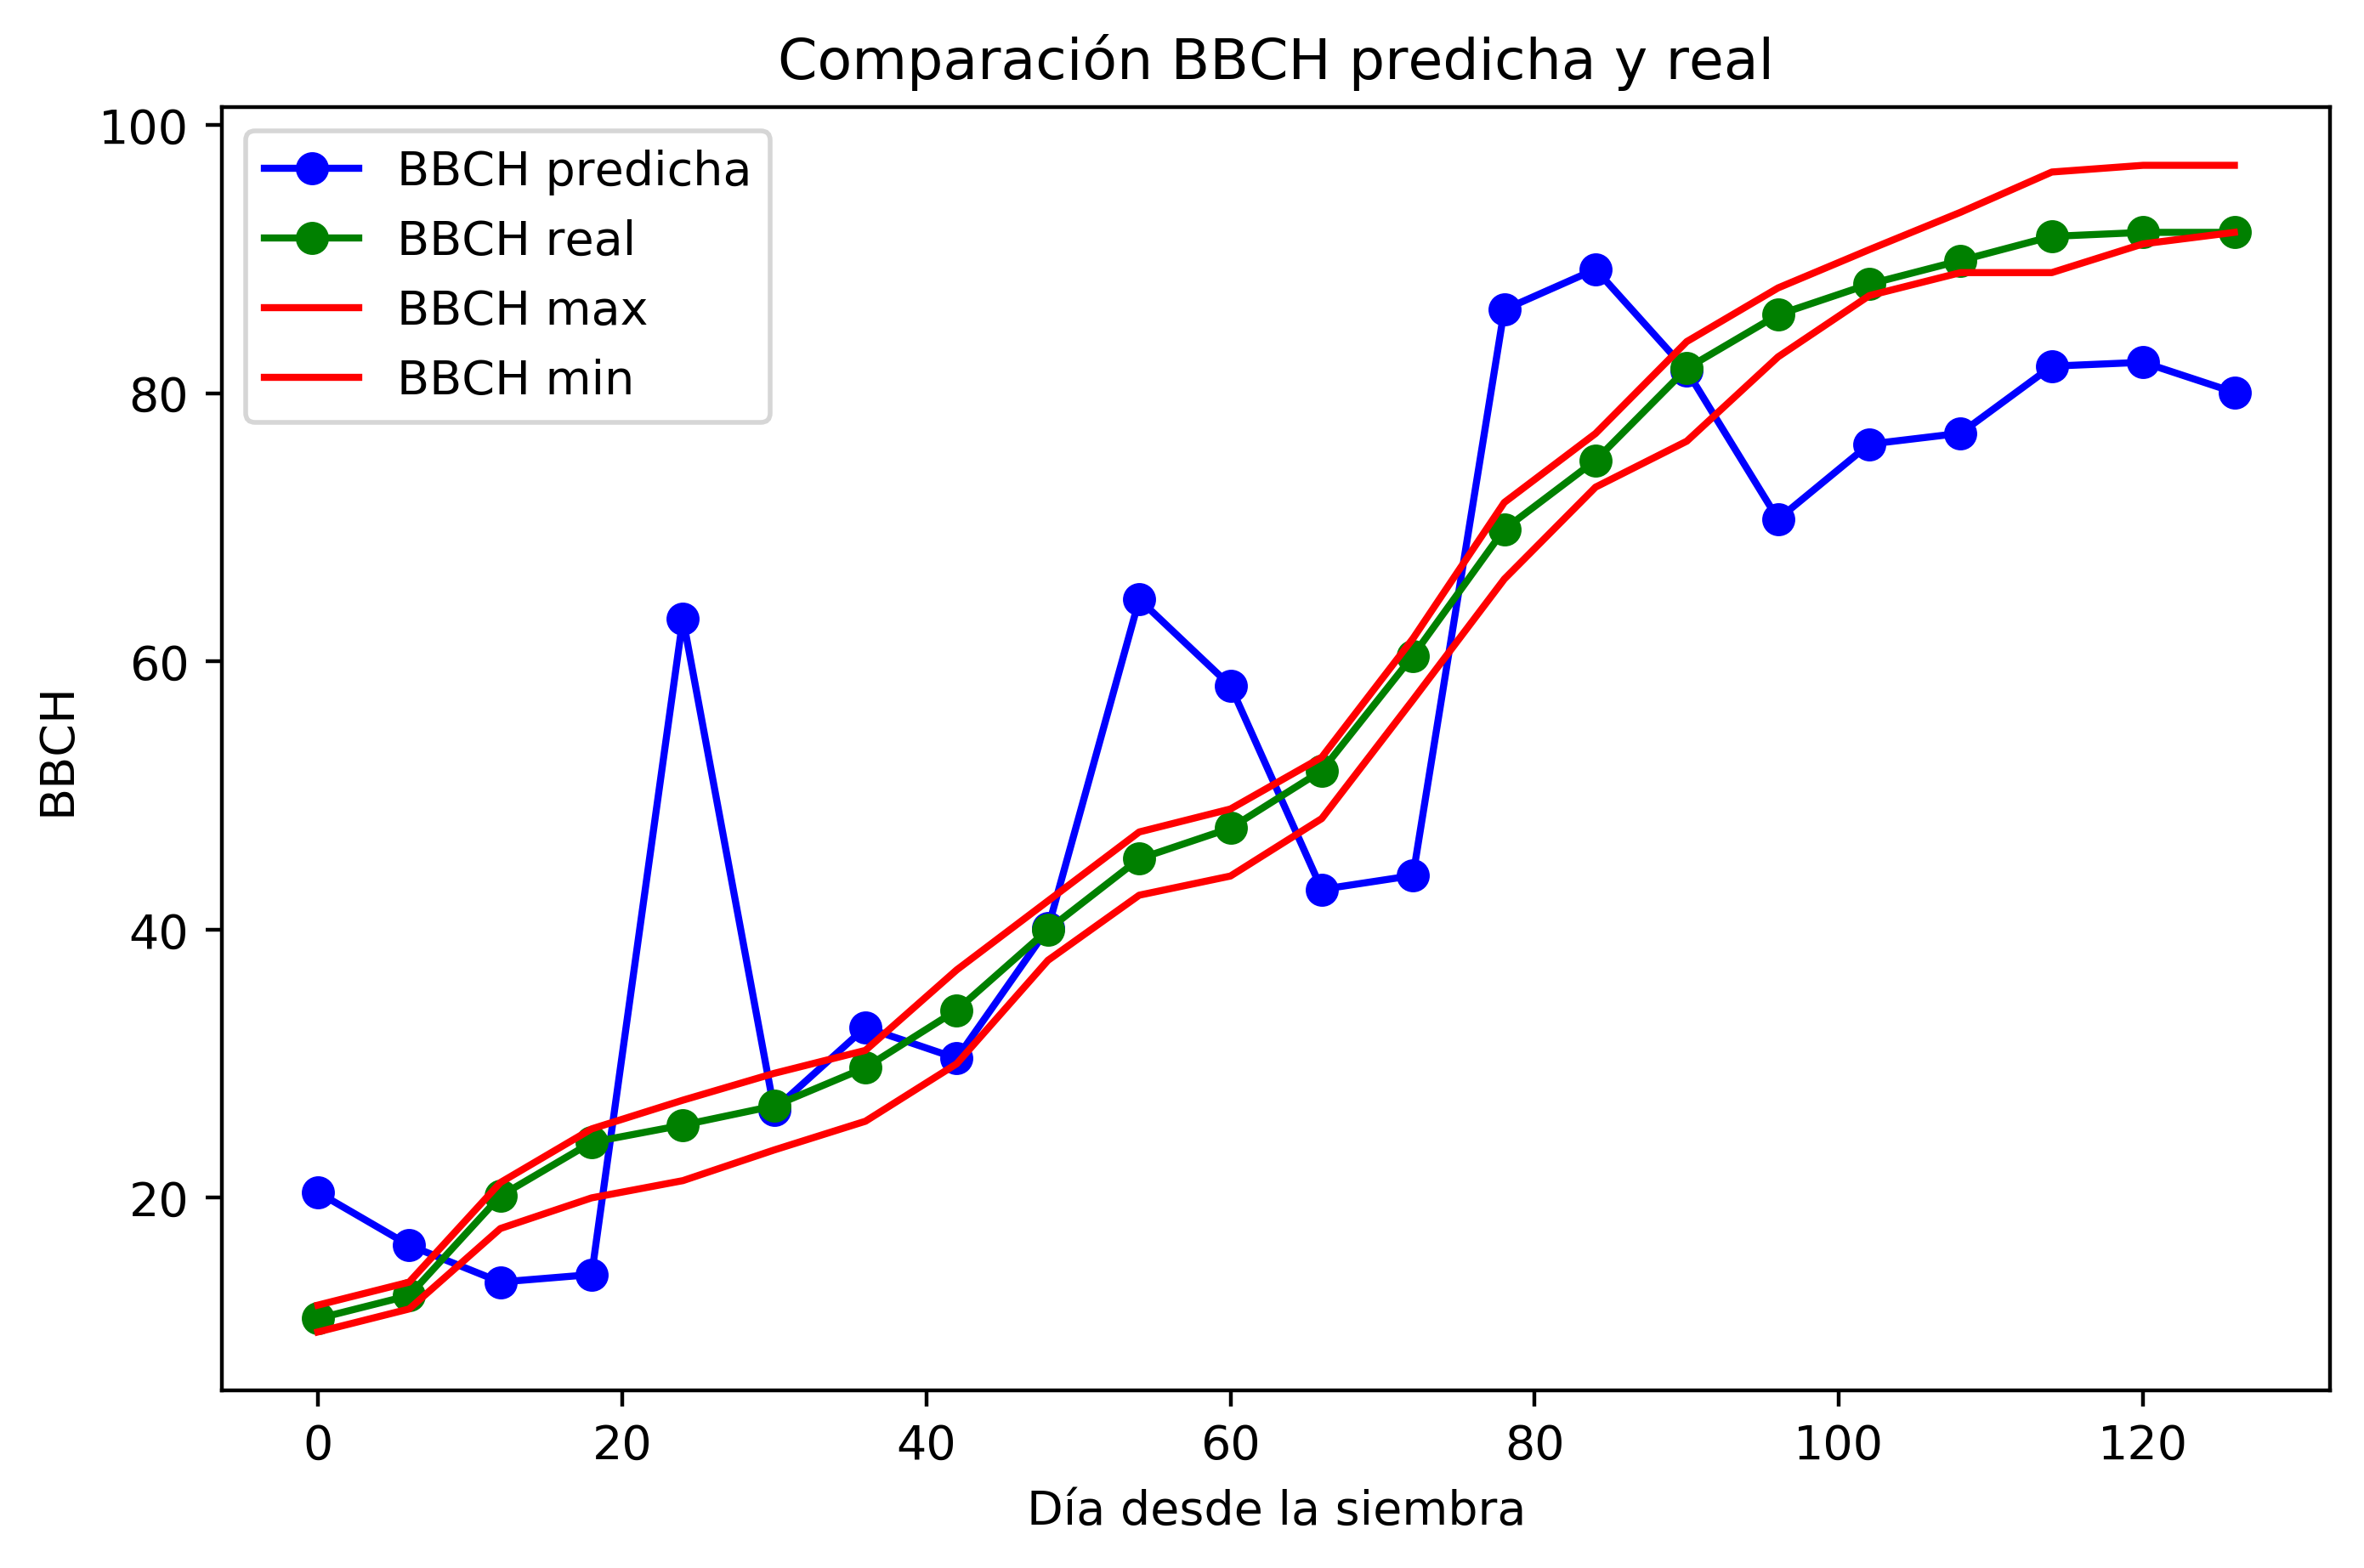
\includegraphics[width=0.95\linewidth]{archivos/tfg/Mean/TEST_PARC_FINAL_BH}
  \caption{Comparación de la salida predicha y la verdad de tierra del modelo de doble salida para la estimación de \gls{bbch}. \label{fig:sub_c1}}
\end{subfigure}
\begin{subfigure}{.65\textwidth}
  \centering
  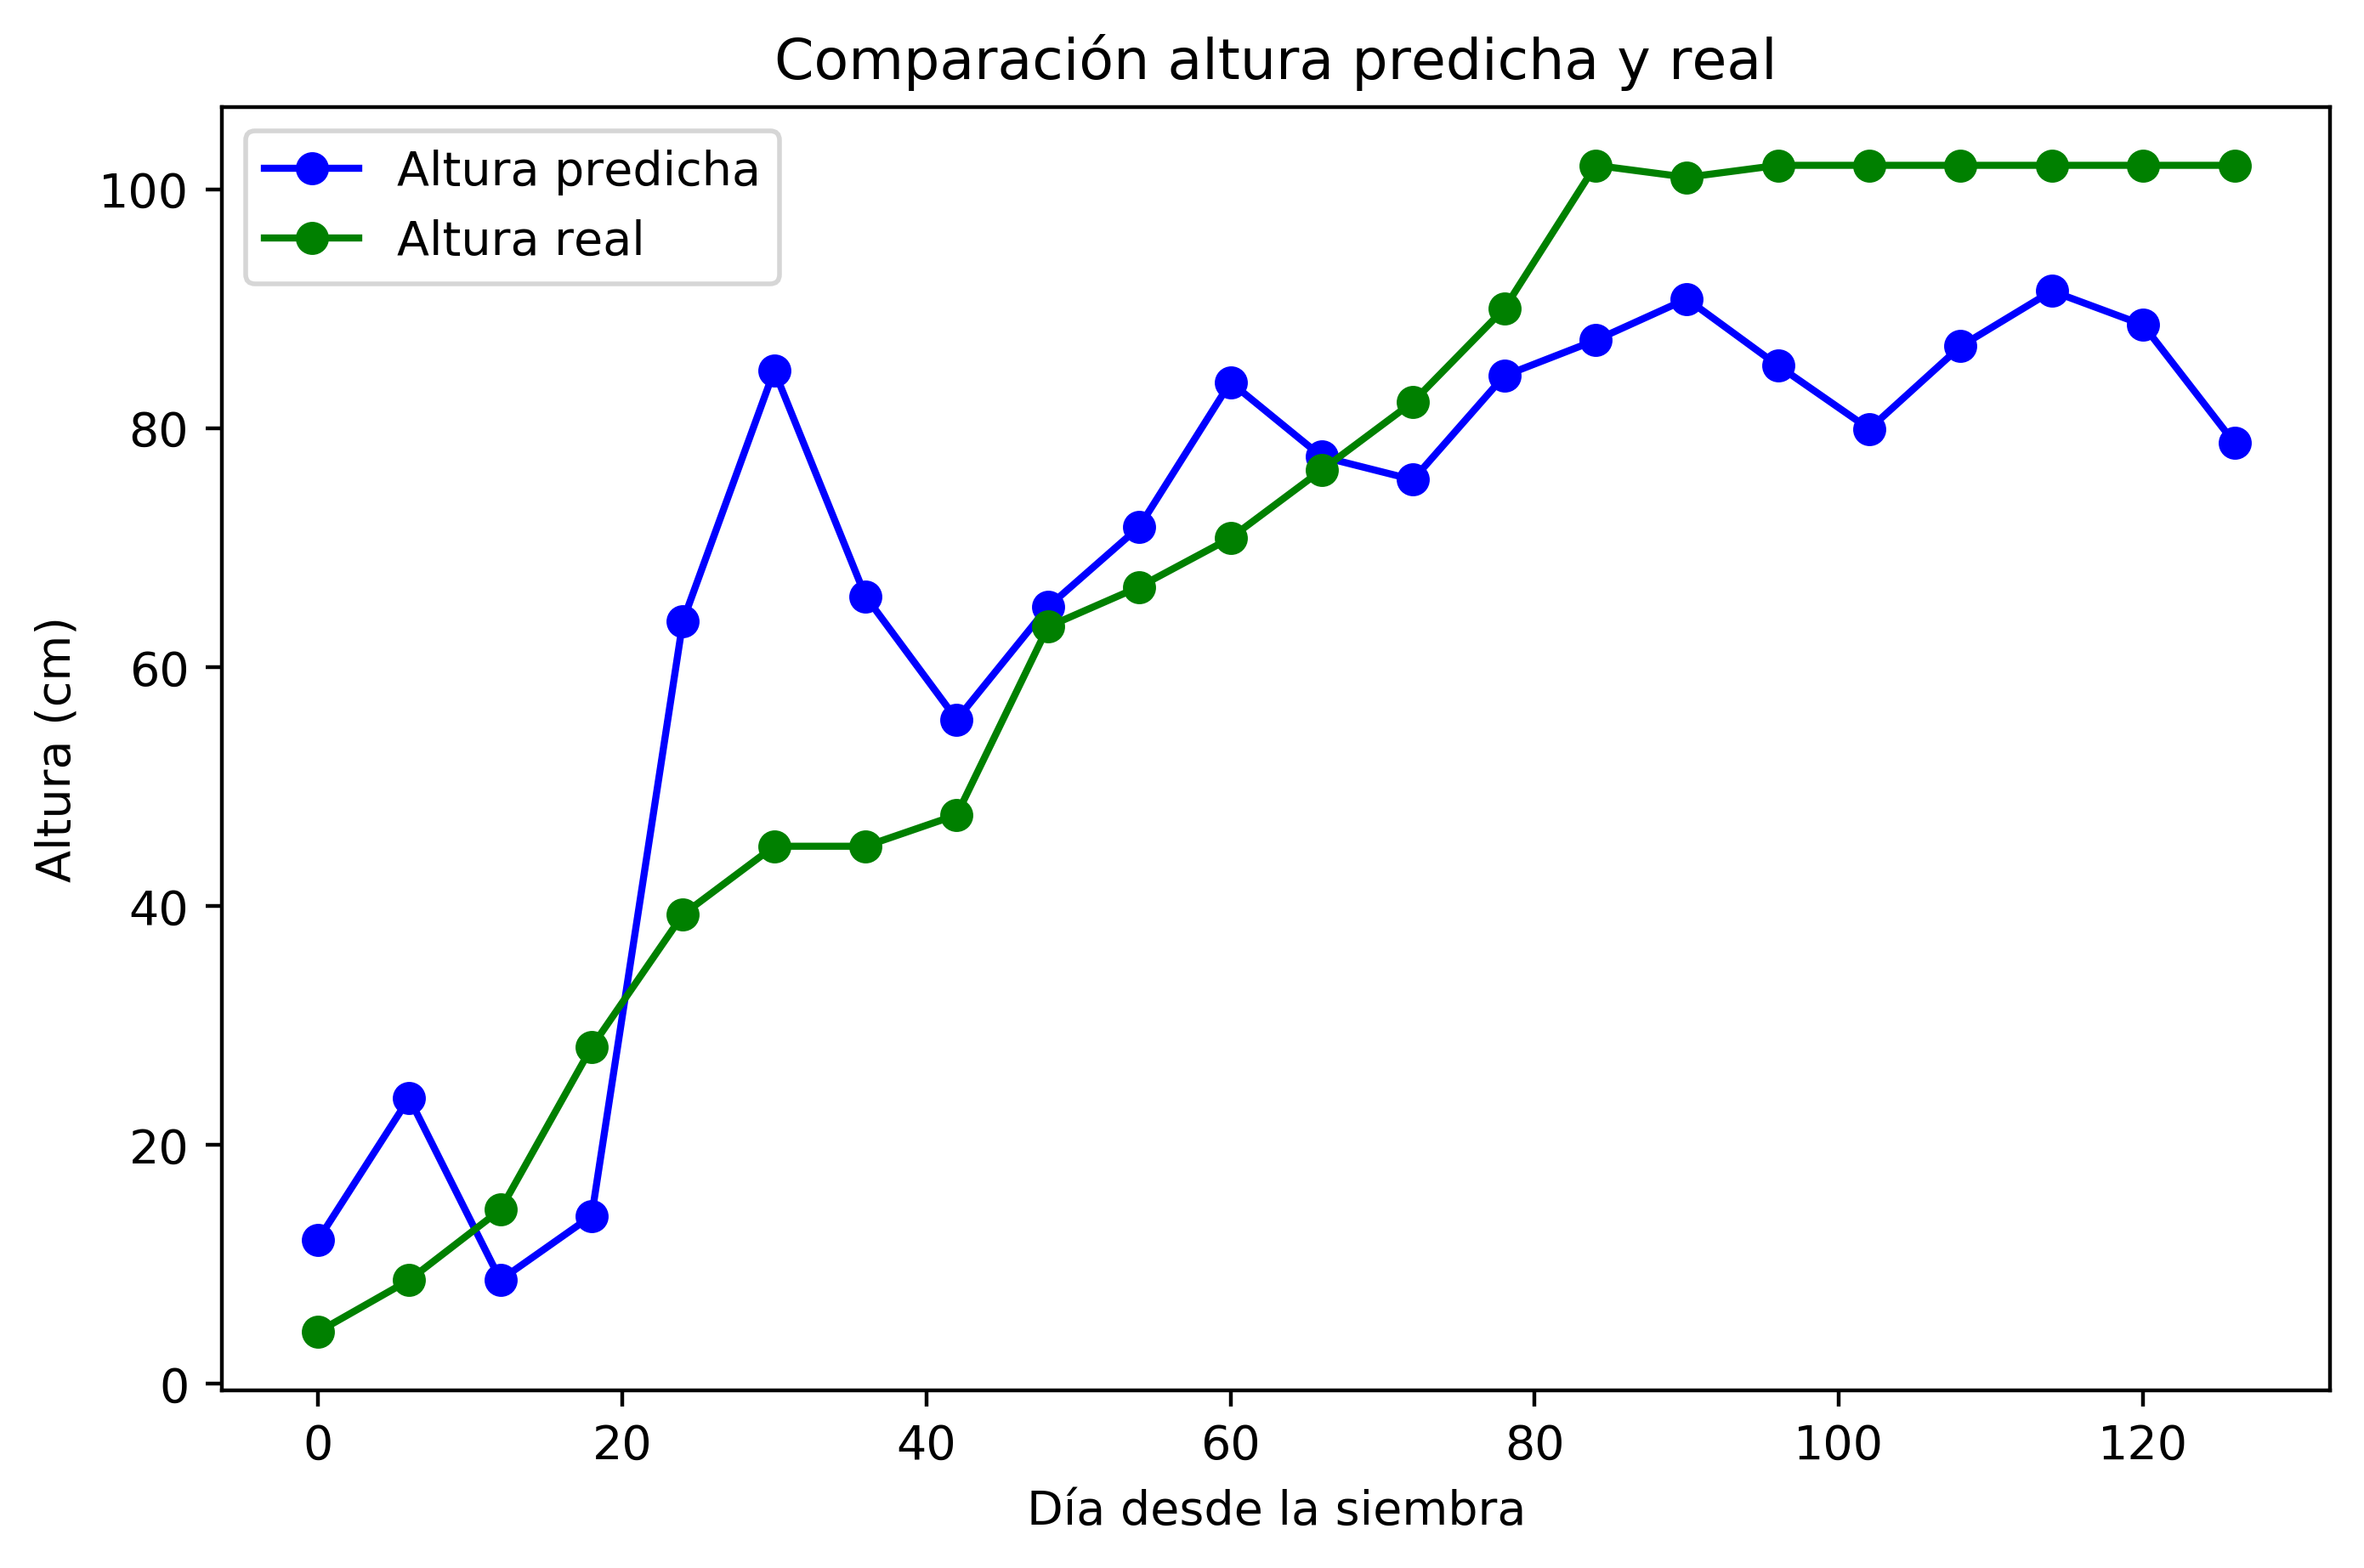
\includegraphics[width=0.95\linewidth]{archivos/tfg/Mean/TEST_PARC_FINAL_BH_H}
  \caption{Comparación de la salida predicha y la verdad de tierra del modelo de doble salida para la estimación de la altura\label{fig:sub_c2}}
\end{subfigure}
\caption{Comparación de la salida predicha y la verdad de tierra del modelo de doble salida para la estimación de \gls{bbch} y la altura. \label{fig:comp_bh}}
\end{figure}

\par Visualizando las salidas para la altura, se puede también comparar, aunque no directamente, el funcionamiento de ambos modelos. En este caso las parcelas de test no son las mismas debido a la optimización para cada modelo, como tampoco los datos de entrada, por lo que la comparación simplemente visual entre las dos representaciones es menos intuitiva. Aún así, se aprecian coincidencias como el error en la etapa cercana a 40 días, como se ha mencionado antes, o la estimación de mayor altura para los días de 0 a 10 después de la siembra. En general, ambas representaciones tienen también una tendencia creciente bastante similar a la real, con aparentemente mejor estimación para las etapas finales en el modelo de salida única de altura, ya que en la figura \ref{fig:comp_h} se observa una estimación menor constante para todas las etapas desde el día 80 tras la siembra hasta la cosecha (día 120 aproximadamente).

\subsection{Evaluación de resultados}
\par Para la evaluación de los resultados obtenidos para el método por parcelas se van a utilizar, como se ha mencionado anteriormente, las salidas de valor único por su facilidad para ser representadas y comparadas con los valores únicos medidos. 
\\
\par La primera evaluación realizada se basa en la relación directa entre las salidas estimadas y las medidas reales, lo cual muestra la fiabilidad del modelo de una forma más clara y así puede verse en las figuras \ref{fig:rel_b}, para el modelo de única salida de \gls{bbch}, \ref{fig:rel_h}, para el modelo de única salida de altura y la figura \ref{fig:rel_bh} para el modelo de doble salida. En estas representaciones se añade, además, una recta de pendiente unidad, la cual sirve de referencia ya que esa relación representaría un ajuste perfecto. Se han utilizado para todas las representaciones los valores contrastados de la parcela de test correspondiente a cada caso, teniendo en cuenta ambos años de datos, 2017 y 2018.

\par En la figura \ref{fig:rel_b} se aprecia una distribución uniforme, lo cuál indica que se disponen de datos suficientes para cubrir las distintas etapas del desarrollo del cultivo. Además, las nubes de puntos se mantienen, en general, cercanos a la recta de referencia, por lo que, excepto para puntos concretos como el pico de las etapas tempranas y las últimas etapas del cultivo, se obtienen resultados bastante buenos. Comparando esta información con la obtenida para el modelo de dos salidas, representado en la figura \ref{fig:rel_bh_b}, se puede asegurar a simple vista qué modelo da mejores resultados. En esta última figura las nubes de puntos se presentan más dispersas que en el anterior, aunque siguiendo la tendencia de la recta de referencia. Vemos, contrariamente, agrupaciones de puntos y huecos, por lo que algunas etapas no están siendo estimadas correctamente. Esto se puede deber al hecho de que el procesamiento de este modelo incluye una etapa de limpieza de datos no válidos que se encuentran en los datos de altura, por lo que en algunas etapas, tanto para la \gls{bbch} como  para la altura, faltan datos que aporten la información completa al sistema. 
\\
\par Comparando a continuación las figuras de los modelos con salida de altura del cultivo, \ref{fig:rel_bh} para salida única y \ref{fig:rel_bh_h} para salida doble, se observa en ambos una mayor inestabilidad en general debida a la concentración de puntos en algunas etapas. La altura de los cultivos no tiene un crecimiento tan lineal progresivo como la fenología de un cultivo, por lo que, a parte de por la corrección de datos, se encuentran concentraciones de datos debido a la estabilidad de la altura durante distintas etapas. Es por ello que, sobre todo en las etapas finales, hay una mayor concentración de puntos, cuando el arroz se mantiene en altura. Aún así, en la figura \ref{fig:rel_bh} se aprecia que todas las estimaciones de altura tienden a la baja para casi todos los datos de altura mayor a 80cm. Una posible explicación sería una tendencia generalizada más baja en las parcelas utilizadas para entrenar el modelo o la poca variación en los parámetros de entrada para alturas desde 50cm hasta 110cm, intervalo en el que la altura estimada se mantiene en torno a la misma franja de valores. 

% Dos figuras sueltas debajo de otra
\begin{figure}[H]
\centering
\begin{subfigure}{0.8\textwidth}
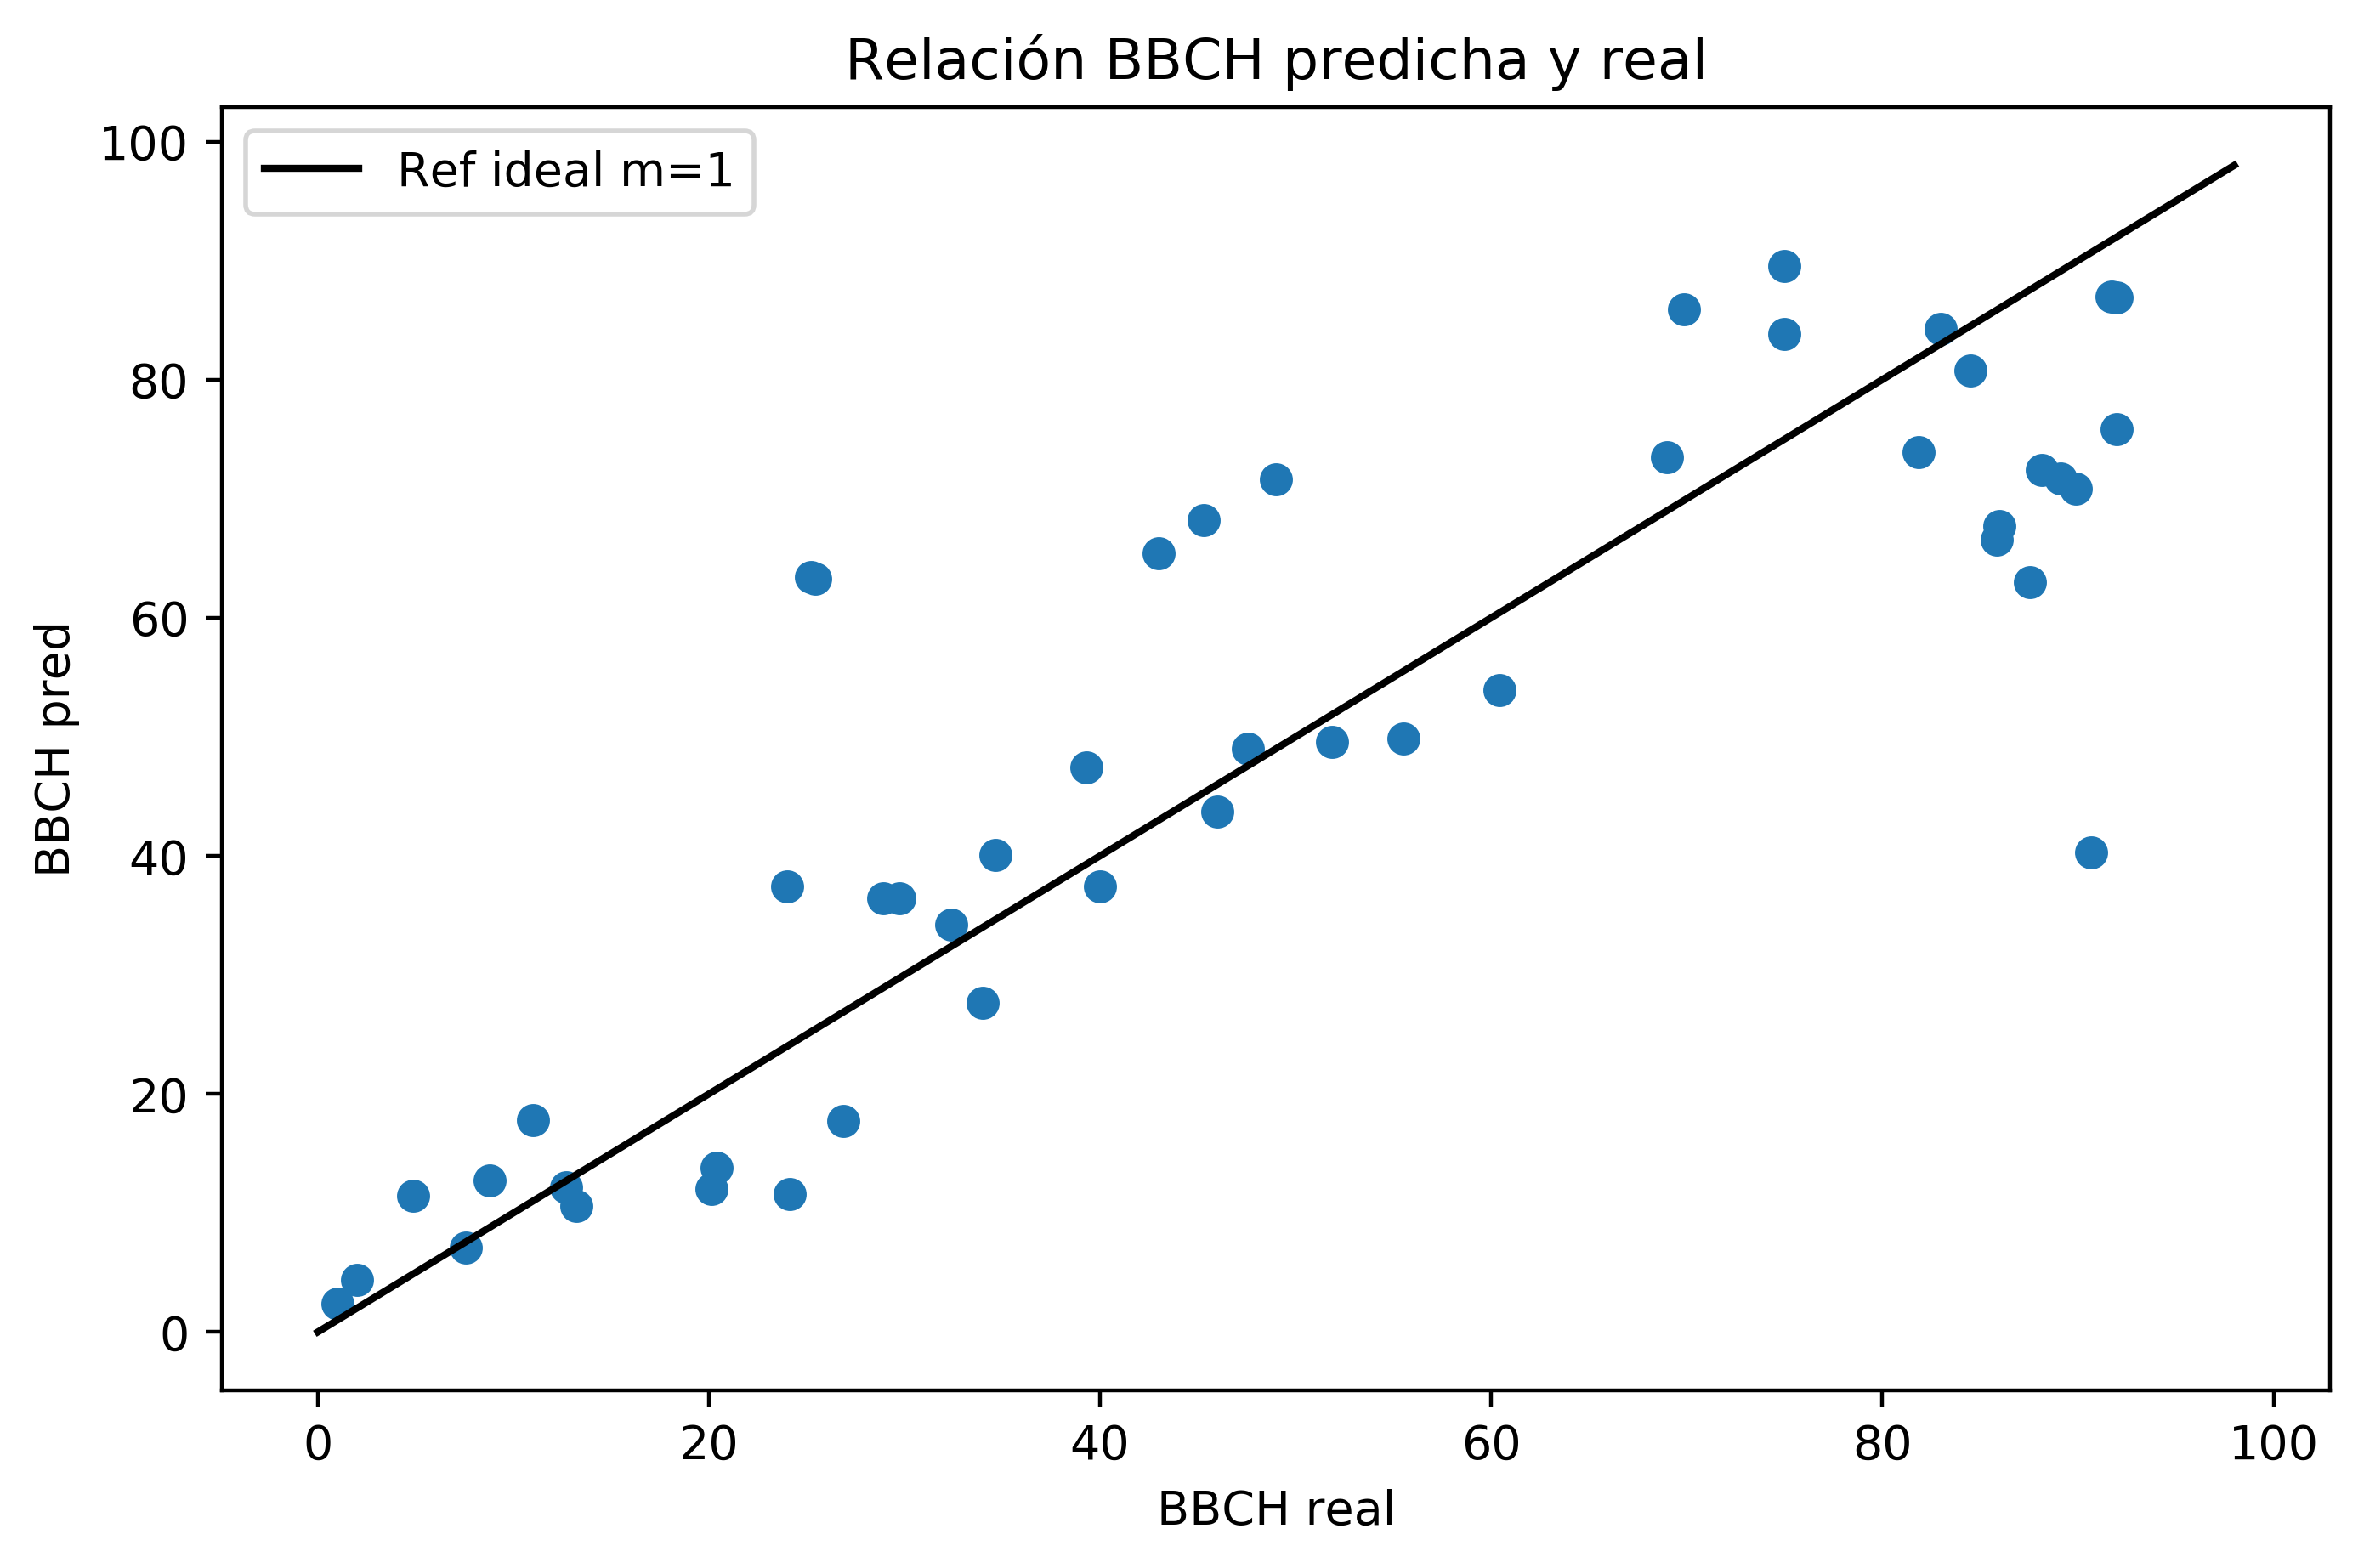
\includegraphics[width=0.95\linewidth]{archivos/tfg/Mean/TEST_PARC_RECTA}
\caption{Relación de la salida predicha y la verdad de tierra del modelo para estimación de \gls{bbch}.\label{fig:rel_b}}
\end{subfigure}
\begin{subfigure}{.8\textwidth}
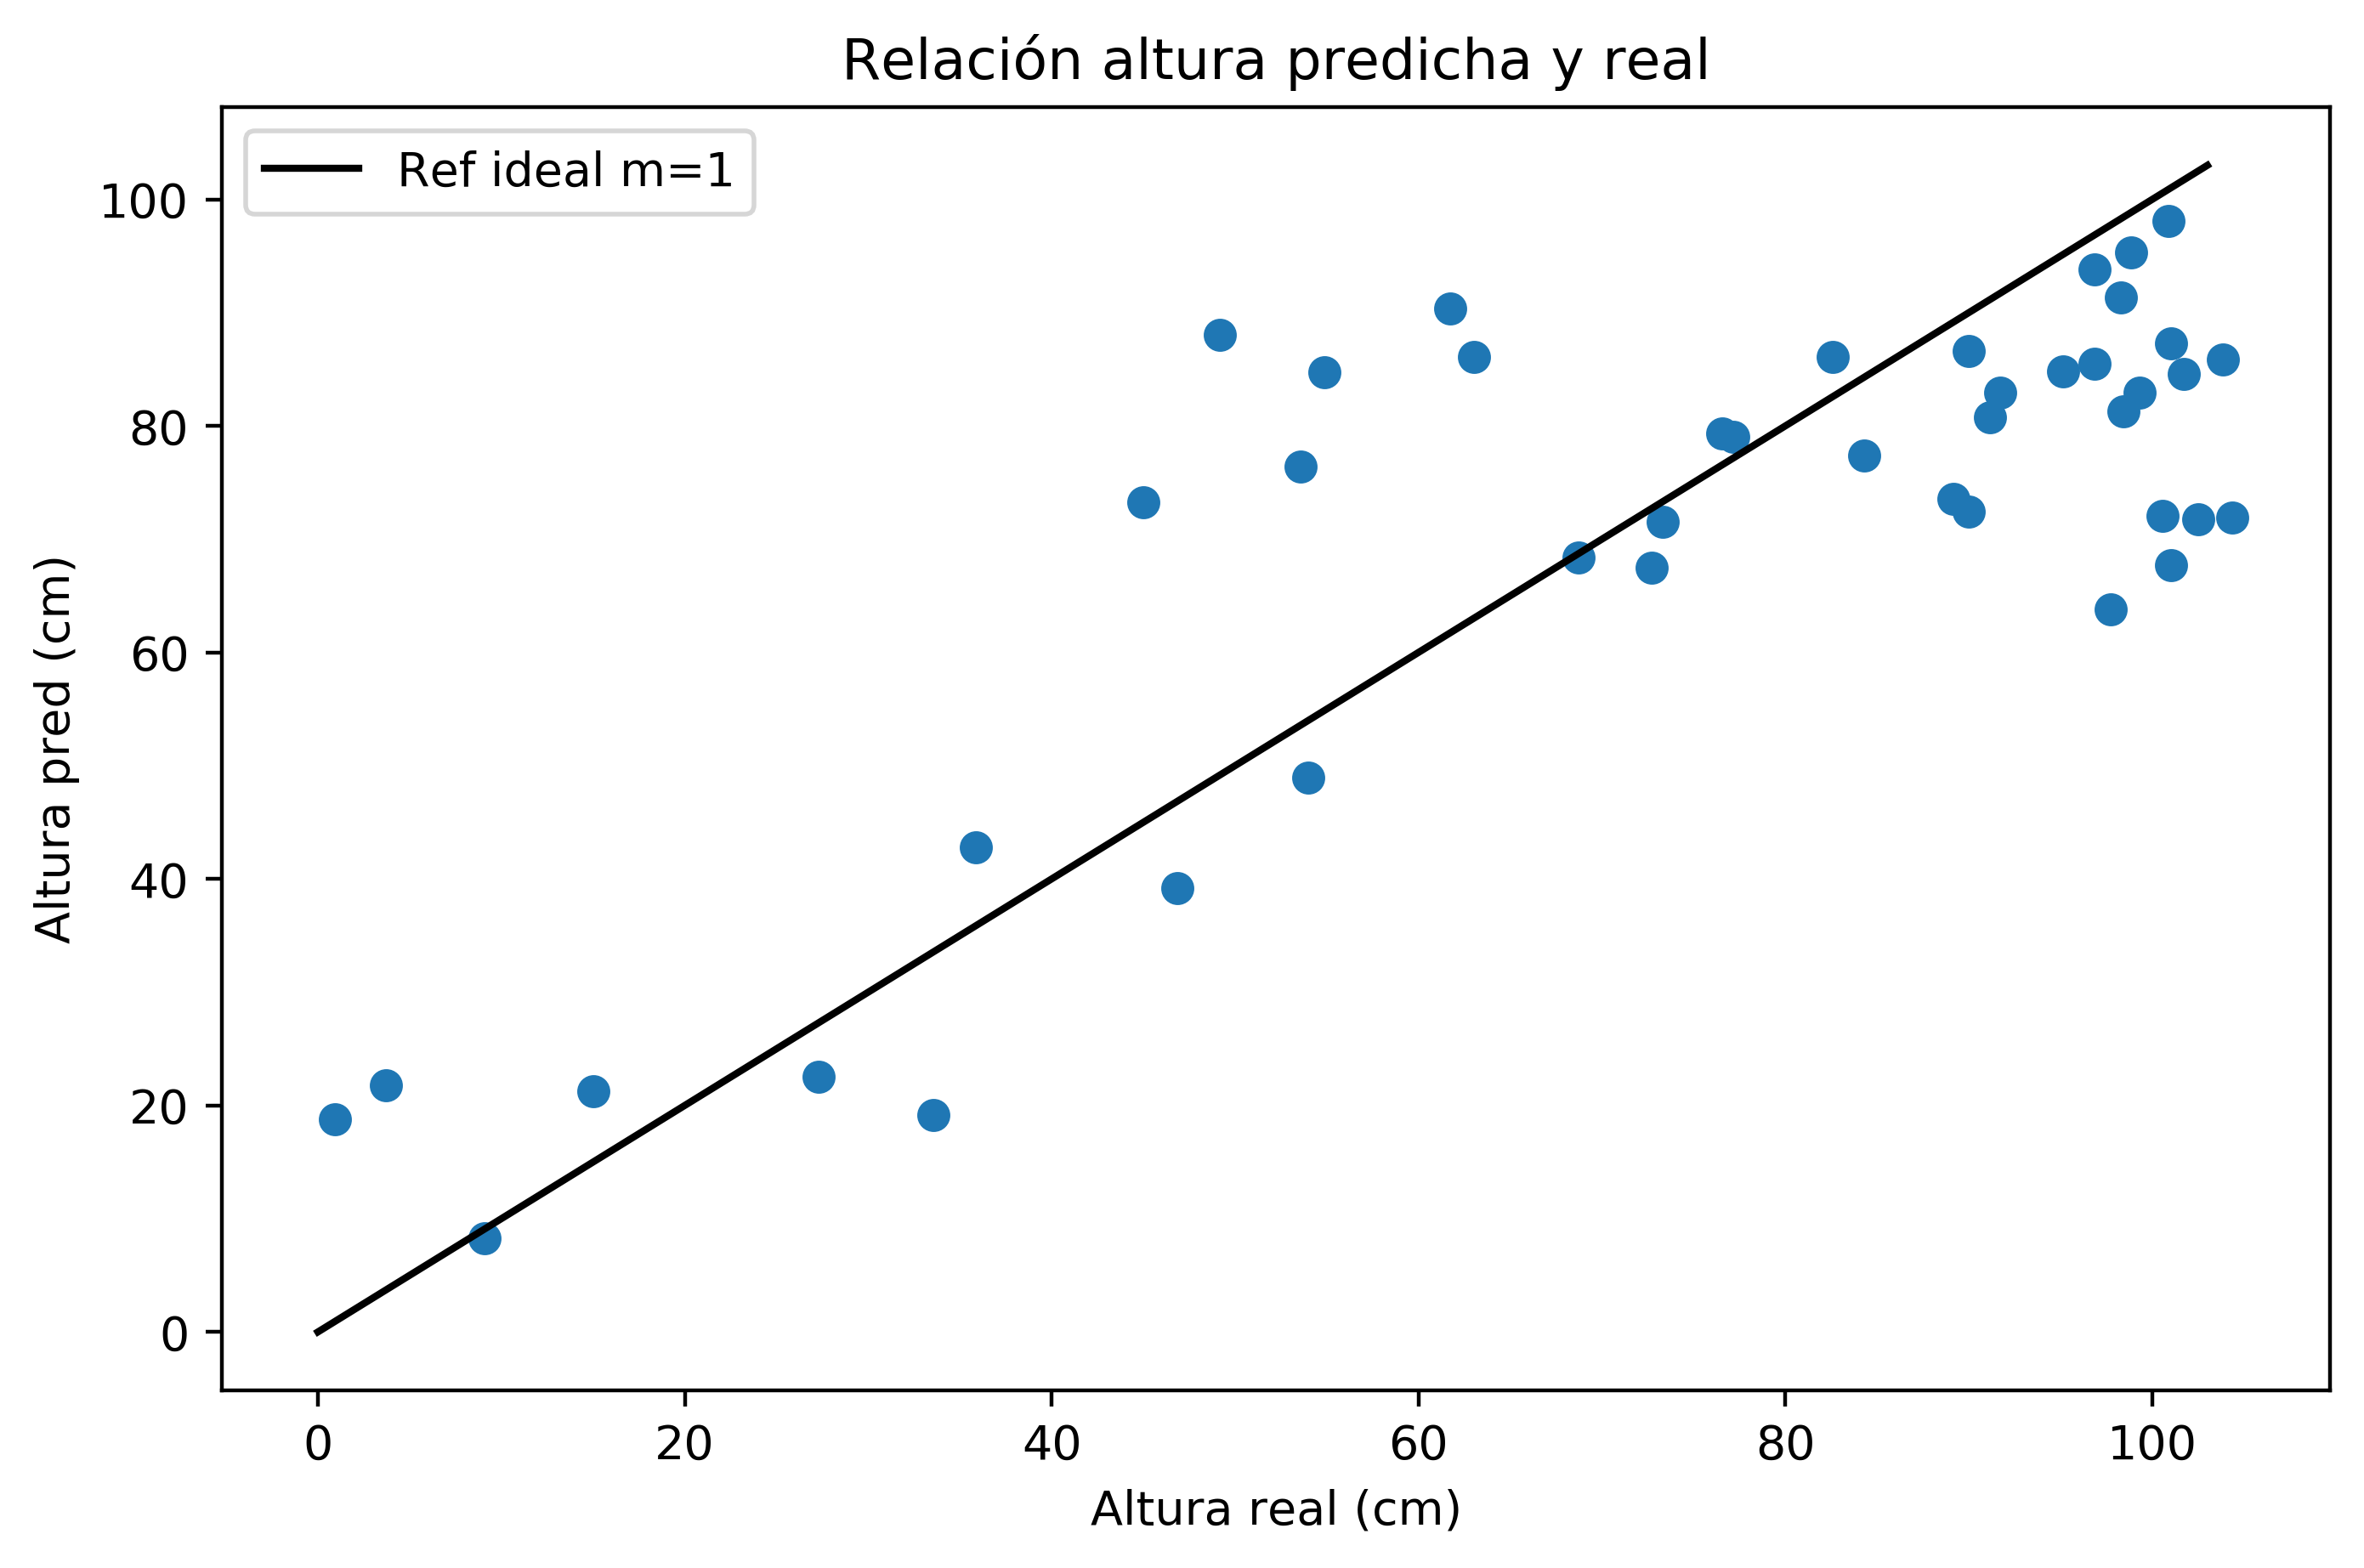
\includegraphics[width=0.95\linewidth]{archivos/tfg/Mean/TEST_PARC_RECTA_H}
\caption{Relación de la salida predicha y la verdad de tierra del modelo para estimación de la altura. \label{fig:rel_h}}
\end{subfigure}
\caption{Relación de la salida predicha y la verdad de tierra de los modelos de variables independientes. \label{fig:rel}}
\end{figure}

% Una figura con dos imágenes
\begin{figure}[H]
\centering
\begin{subfigure}{.8\textwidth}
  \centering
  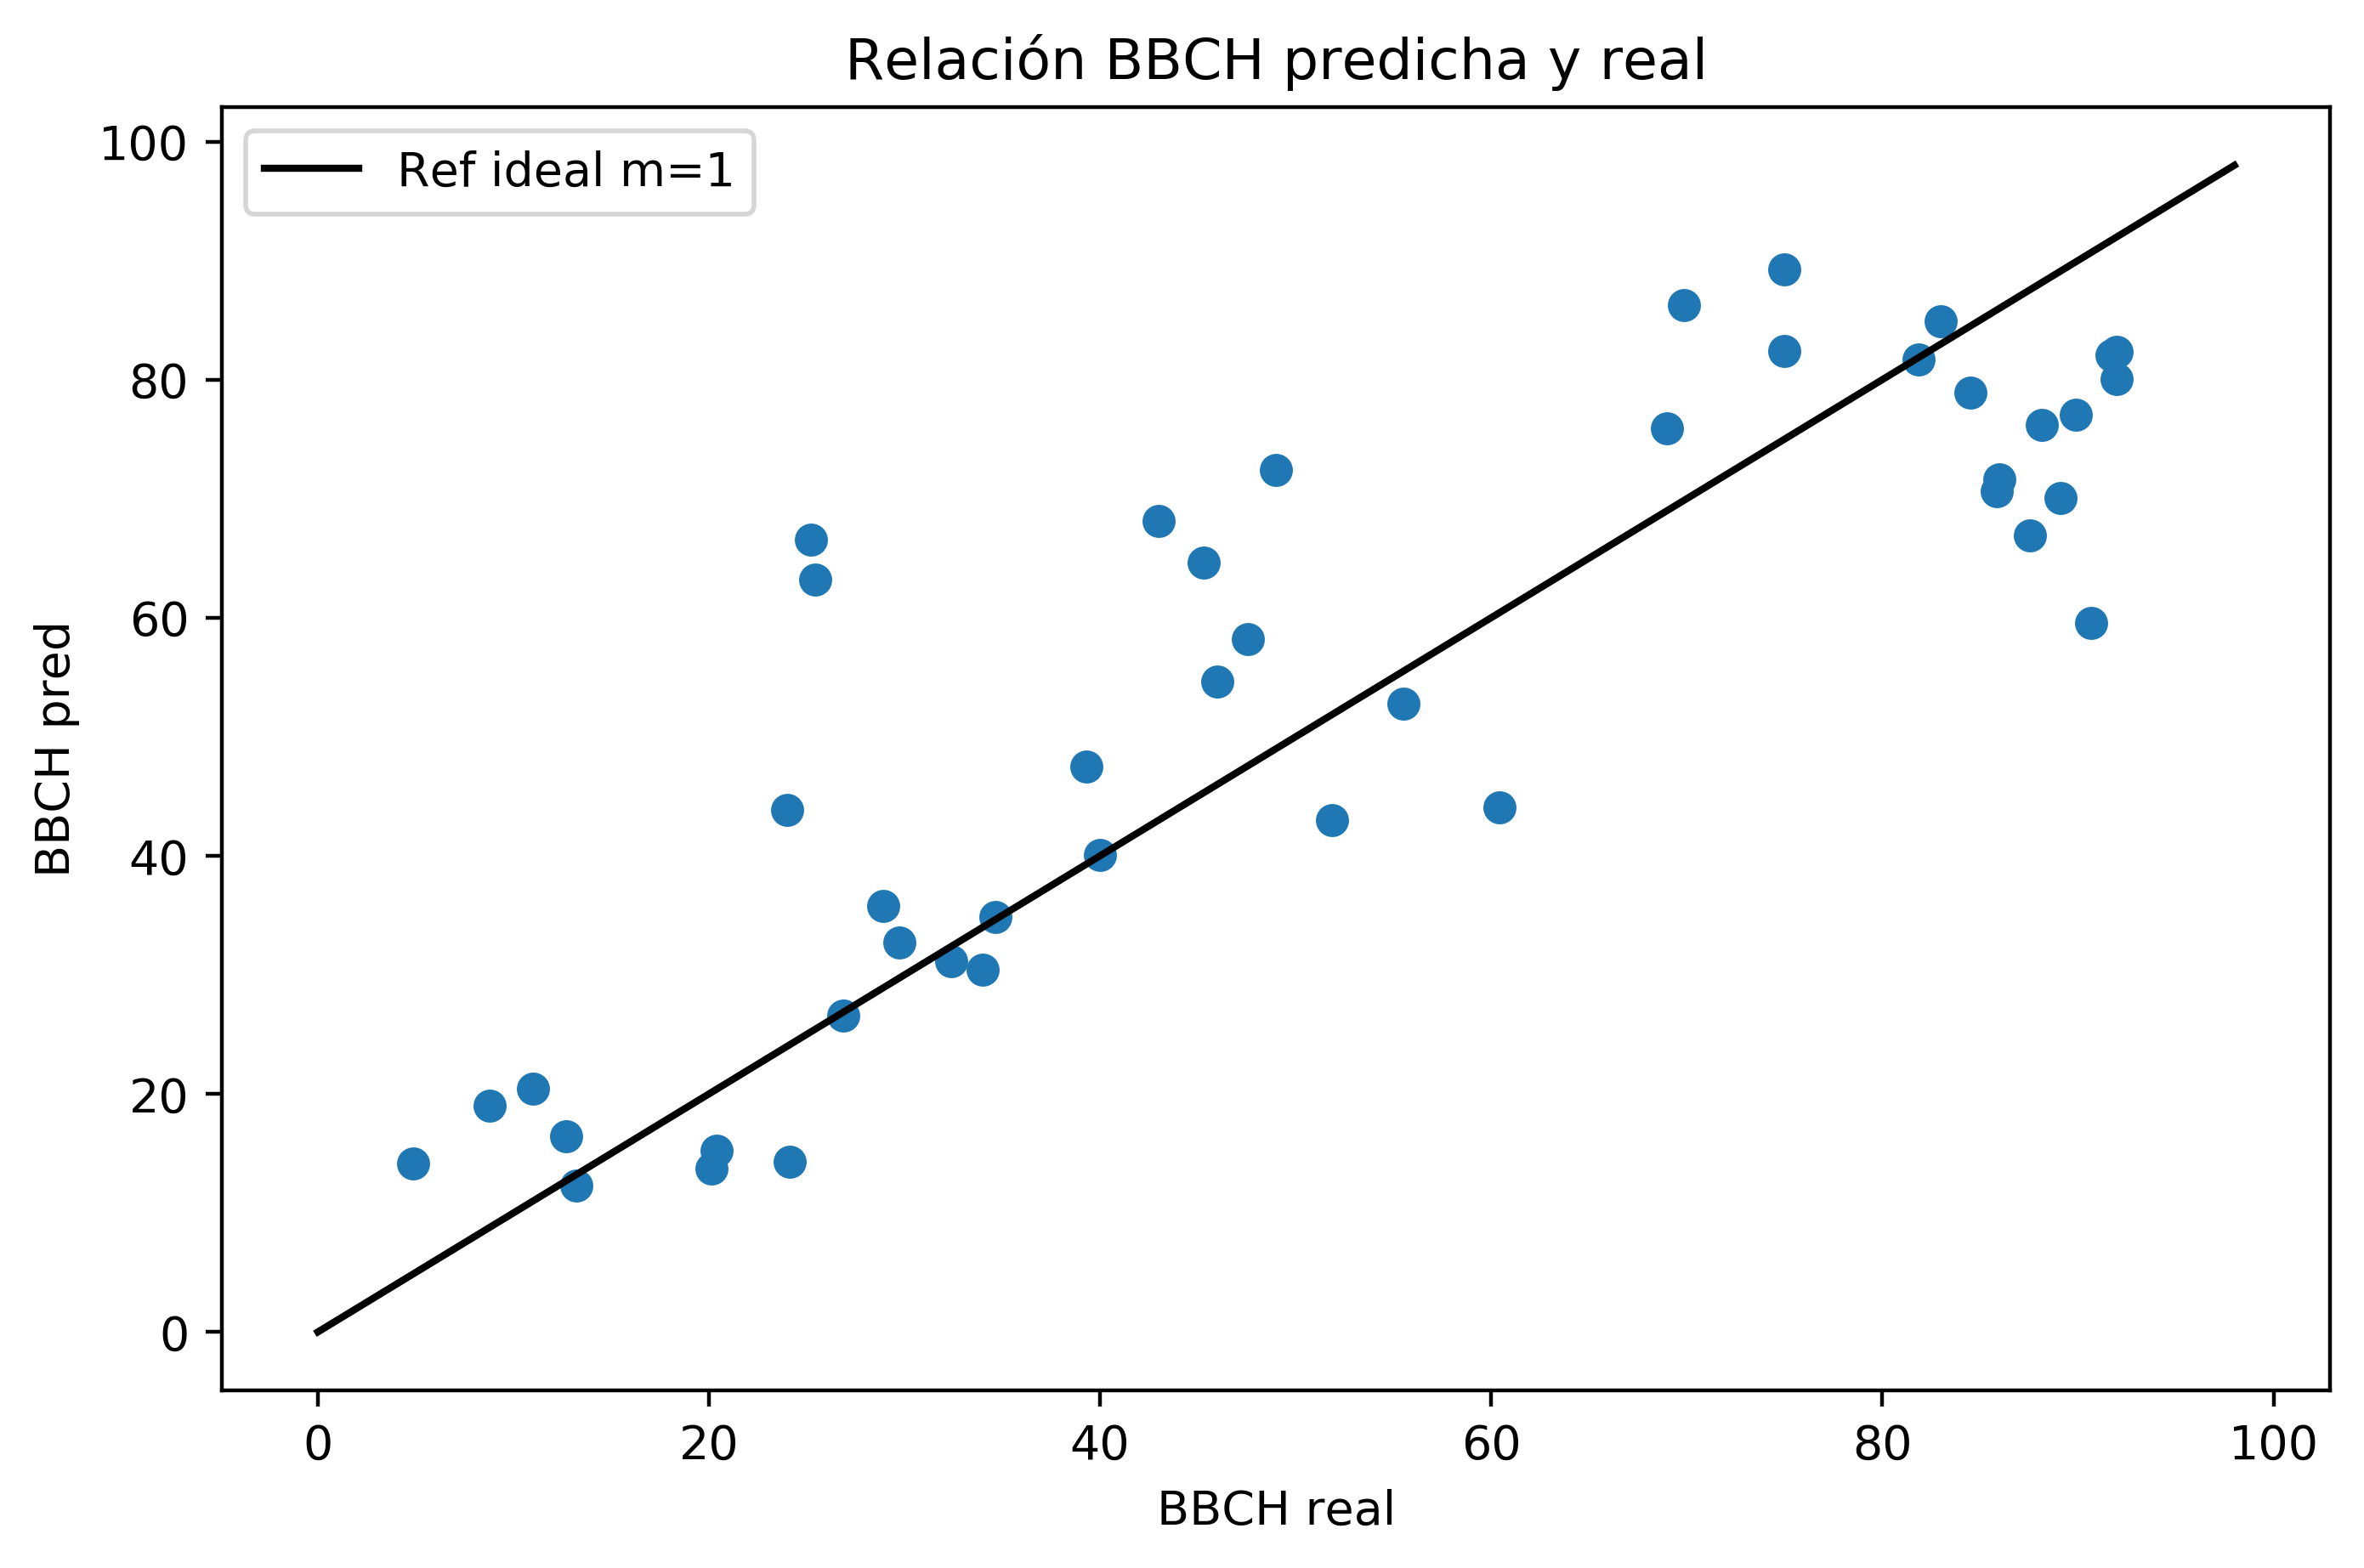
\includegraphics[width=0.95\linewidth]{archivos/tfg/Mean/TEST_PARC_RECTA_bh}
  \caption{Relación de la salida predicha y la verdad de tierra del modelo de doble salida para la estimación de \gls{bbch}. \label{fig:rel_bh_b}}
\end{subfigure}
\begin{subfigure}{.8\textwidth}
  \centering
  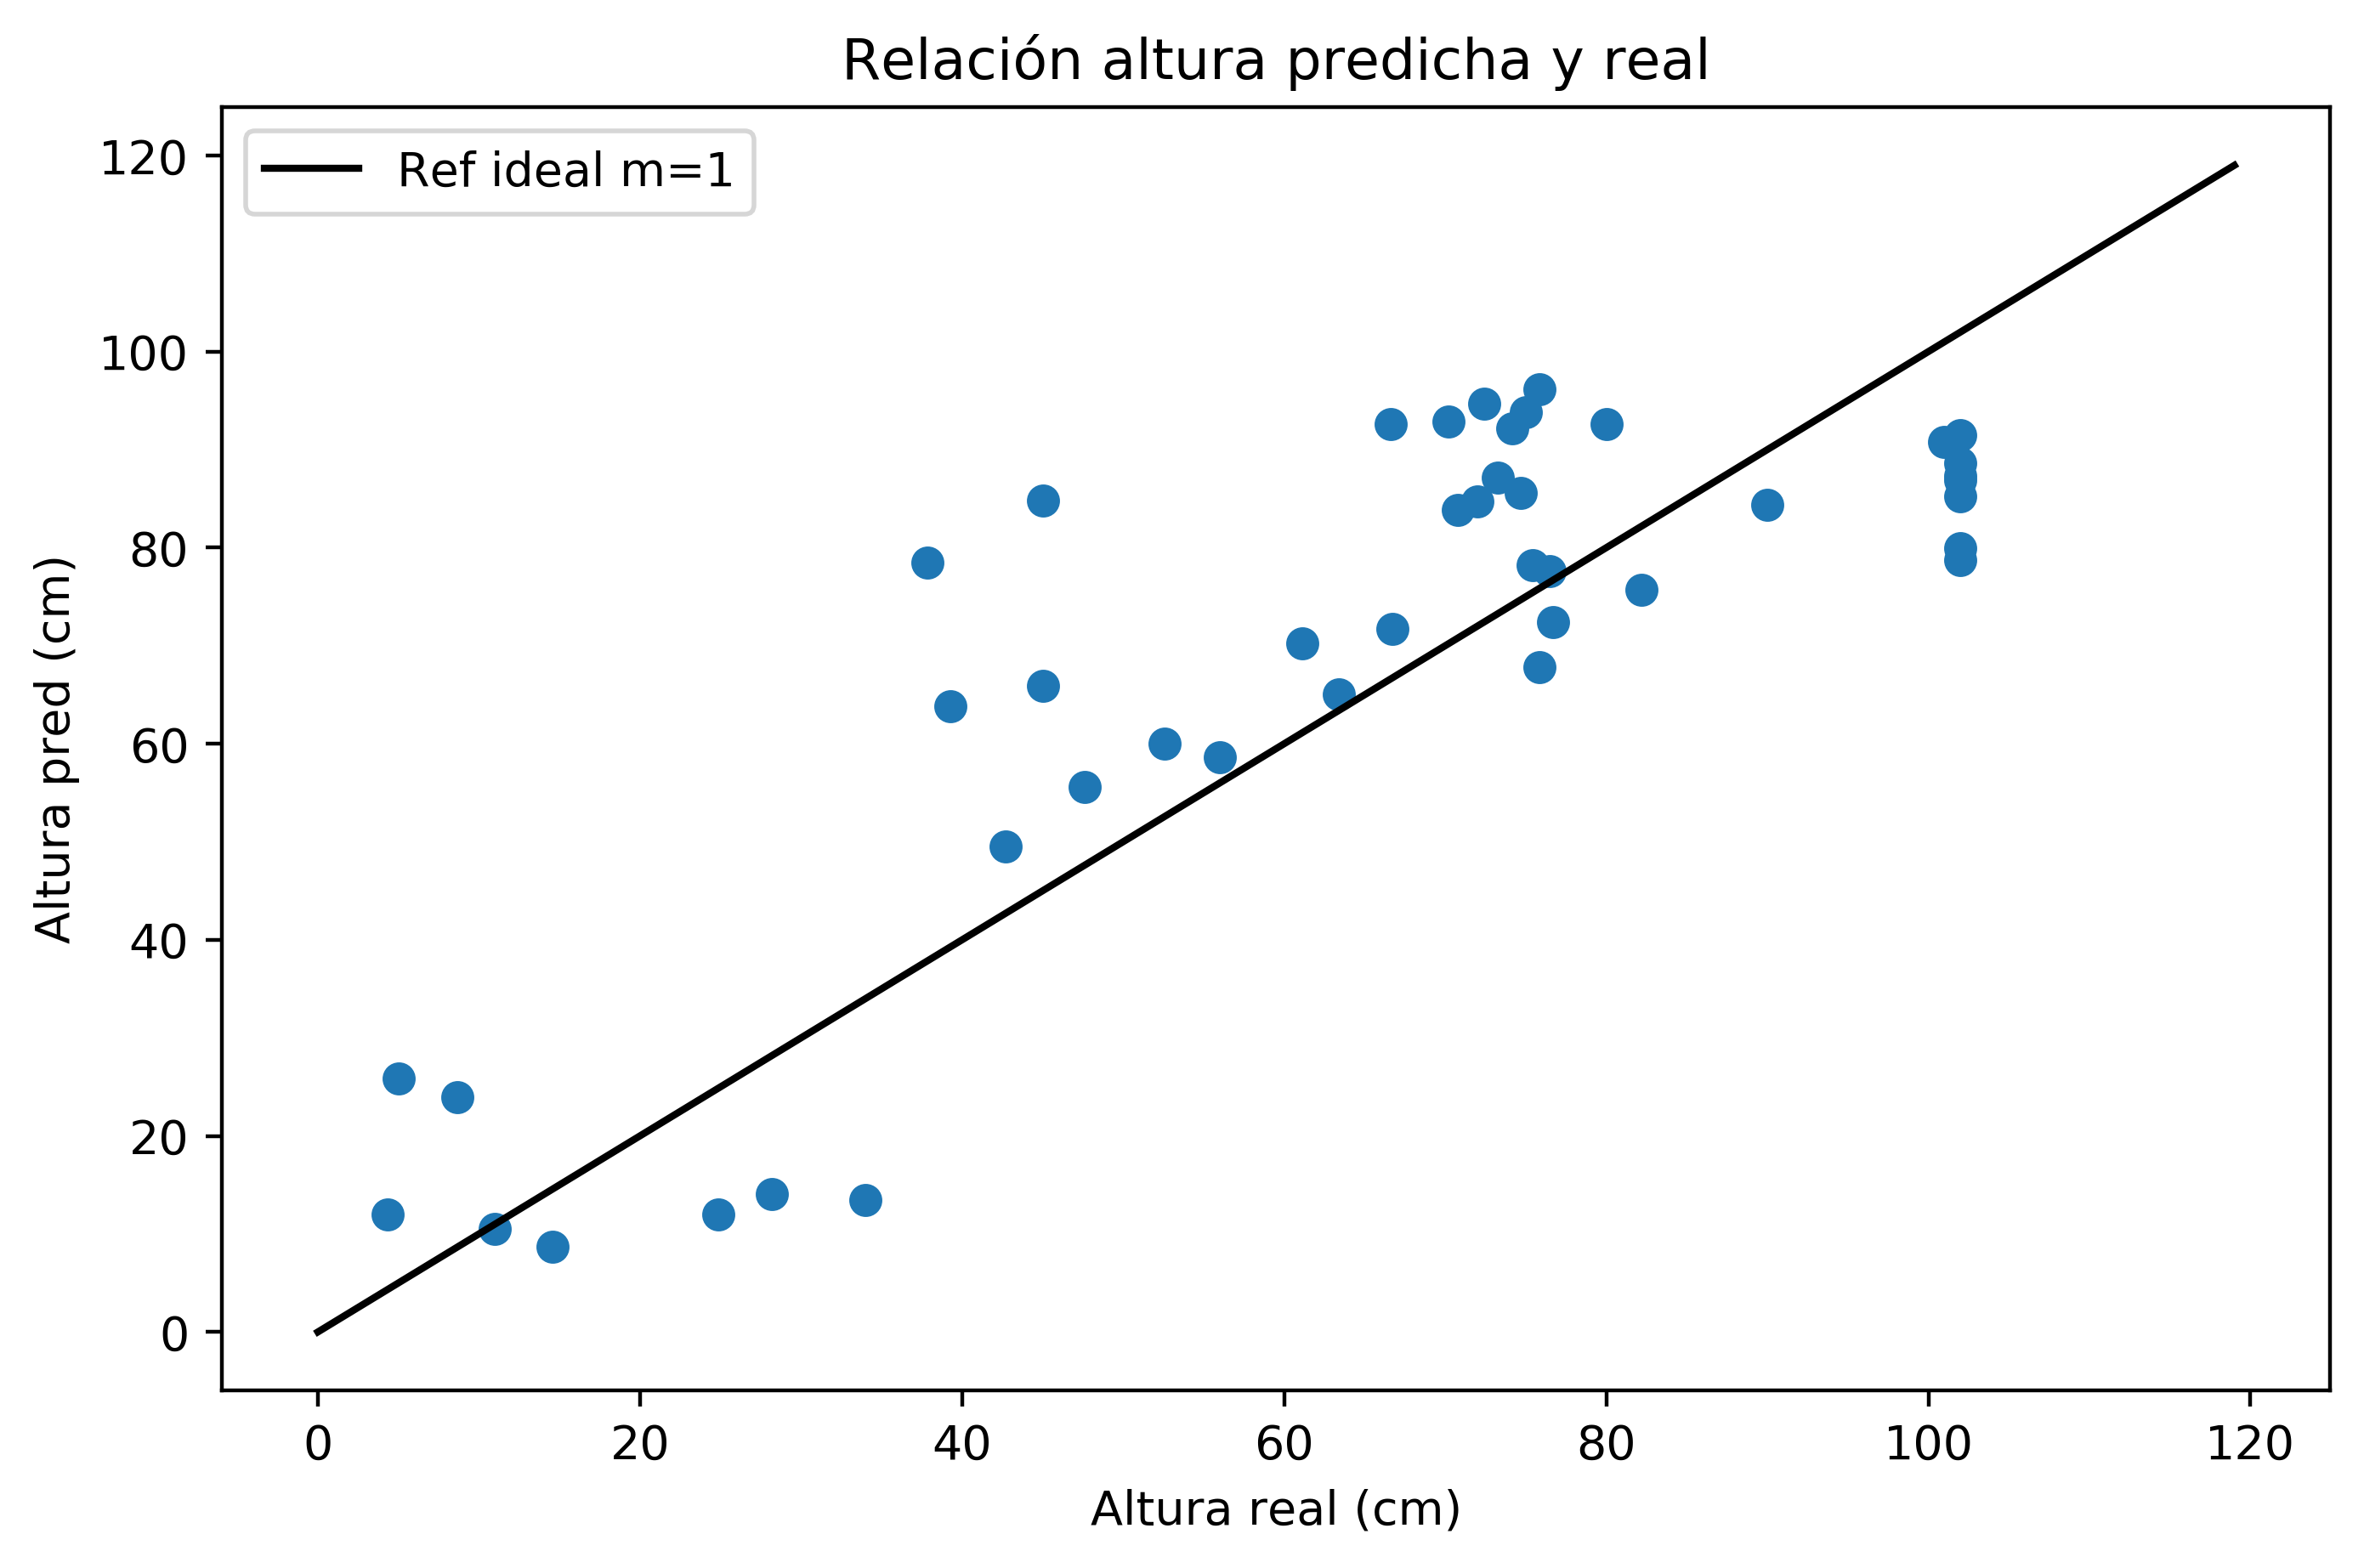
\includegraphics[width=0.95\linewidth]{archivos/tfg/Mean/TEST_PARC_RECTA_bh_H}
  \caption{Relación de la salida predicha y la verdad de tierra del modelo de doble salida para la estimación de la altura\label{fig:rel_bh_h}}
\end{subfigure}
\caption{Relación de la salida predicha y la verdad de tierra del modelo de doble salida para la estimación de \gls{bbch} y la altura. \label{fig:rel_bh}}
\end{figure}

\par A parte de la evaluación con descriptores estadísticos que se realizan a la hora de comparar los dos métodos, se realiza también una evaluación de los datos de entrada utilizados. La tabla \ref{tab:imp_f} representa el peso que tiene cada una de las variables de entrada en el modelo generado para cada uno de los 3 casos tratados. 
\\
\begin{table}[h] 
\centering
\begin{tabular}{l|ccc}
               & \gls{bbch} & Altura & \gls{bbch}\&Altura \\ \hline \hline
VV             & 0.12 & 0.17   & 0.12         \\
VH             & 0.52 & 0.69   & 0.53         \\
Ratio VH/VV    & 0.11 & 0.14   & 0.10         \\
Dev est. VV    & 0.09 & -   & 0.10         \\
Dev est. VH    & 0.07 & -   & 0.09         \\
Dev est. ratio & 0.07 & -   & 0.06        
\end{tabular}
\caption{Influencia de los parámetros de entrada en el modelo de estimación.\label{tab:imp_f}}
\end{table}

\par En la tabla \ref{tab:imp_f} se presentan proporciones altamente similares para los 2 casos con las mismas entradas, y proporcionalmente parecidos para el caso de predicción de la altura. El parámetro de entrada que destaca principalmente sobre el resto es el coeficiente de backscattering para la polarización VH, con más del 50\% de la predicción elaborada en base a él. Los siguientes parámetros más influyentes son el coeficiente de backscattering para la polarización VV y el ratio de ambos, y, por último, las desviaciones estándar, que suponen menos del 10\% de la predicción final. Para comprender mejor porqué existen estas diferencias, se representan en la figura \ref{fig:rel_param} la relación entre cada una de las variables con \gls{bbch}.
\\
\par Lo primero que se observa en la figura \ref{fig:rel_param} es que todas las subfiguras, en general, presentan una tendencia creciente conforme \gls{bbch} va creciendo, que a los primeros estados corresponden valores más bajos y que en todas aparece el pico de detección entorno a un valor de \gls{bbch} de 20-30, que se asemeja a los valores obtenidos por los mismos parámetros para \gls{bbch} cercanas a la cosecha. Esto confirma que las predicciones erróneas cercanas a estas etapas vienen dadas por esta anomalía a la que se le podría buscar corrección. 
\\
\par Comparando los valores que se obtienen para los distintos parámetros a partir de una \gls{bbch} de 40, se aprecia en la subfigura \ref{fig:VH} que su evolución es la más estable y además creciente. Esto quiere decir que, al contrario que en las subfiguras \ref{fig:VV} y \ref{fig:RATIO}, no hay oscilaciones en los valores de entrada y, por tanto, la predicción a partir de estos valores es más sencilla que si para un mismo valor de entrada pueden corresponder distintas \gls{bbch} o alturas. Además, estas etapas finales en la subfigura \ref{fig:VH} se presentan estables pero no constantes, que sería el peor caso que se puede hallar, ya que no aportaría ninguna distinción para intervalos de \gls{bbch} muy amplios. 

\begin{figure}[H]
\centering
\begin{subfigure}{.45\textwidth}
  \centering
  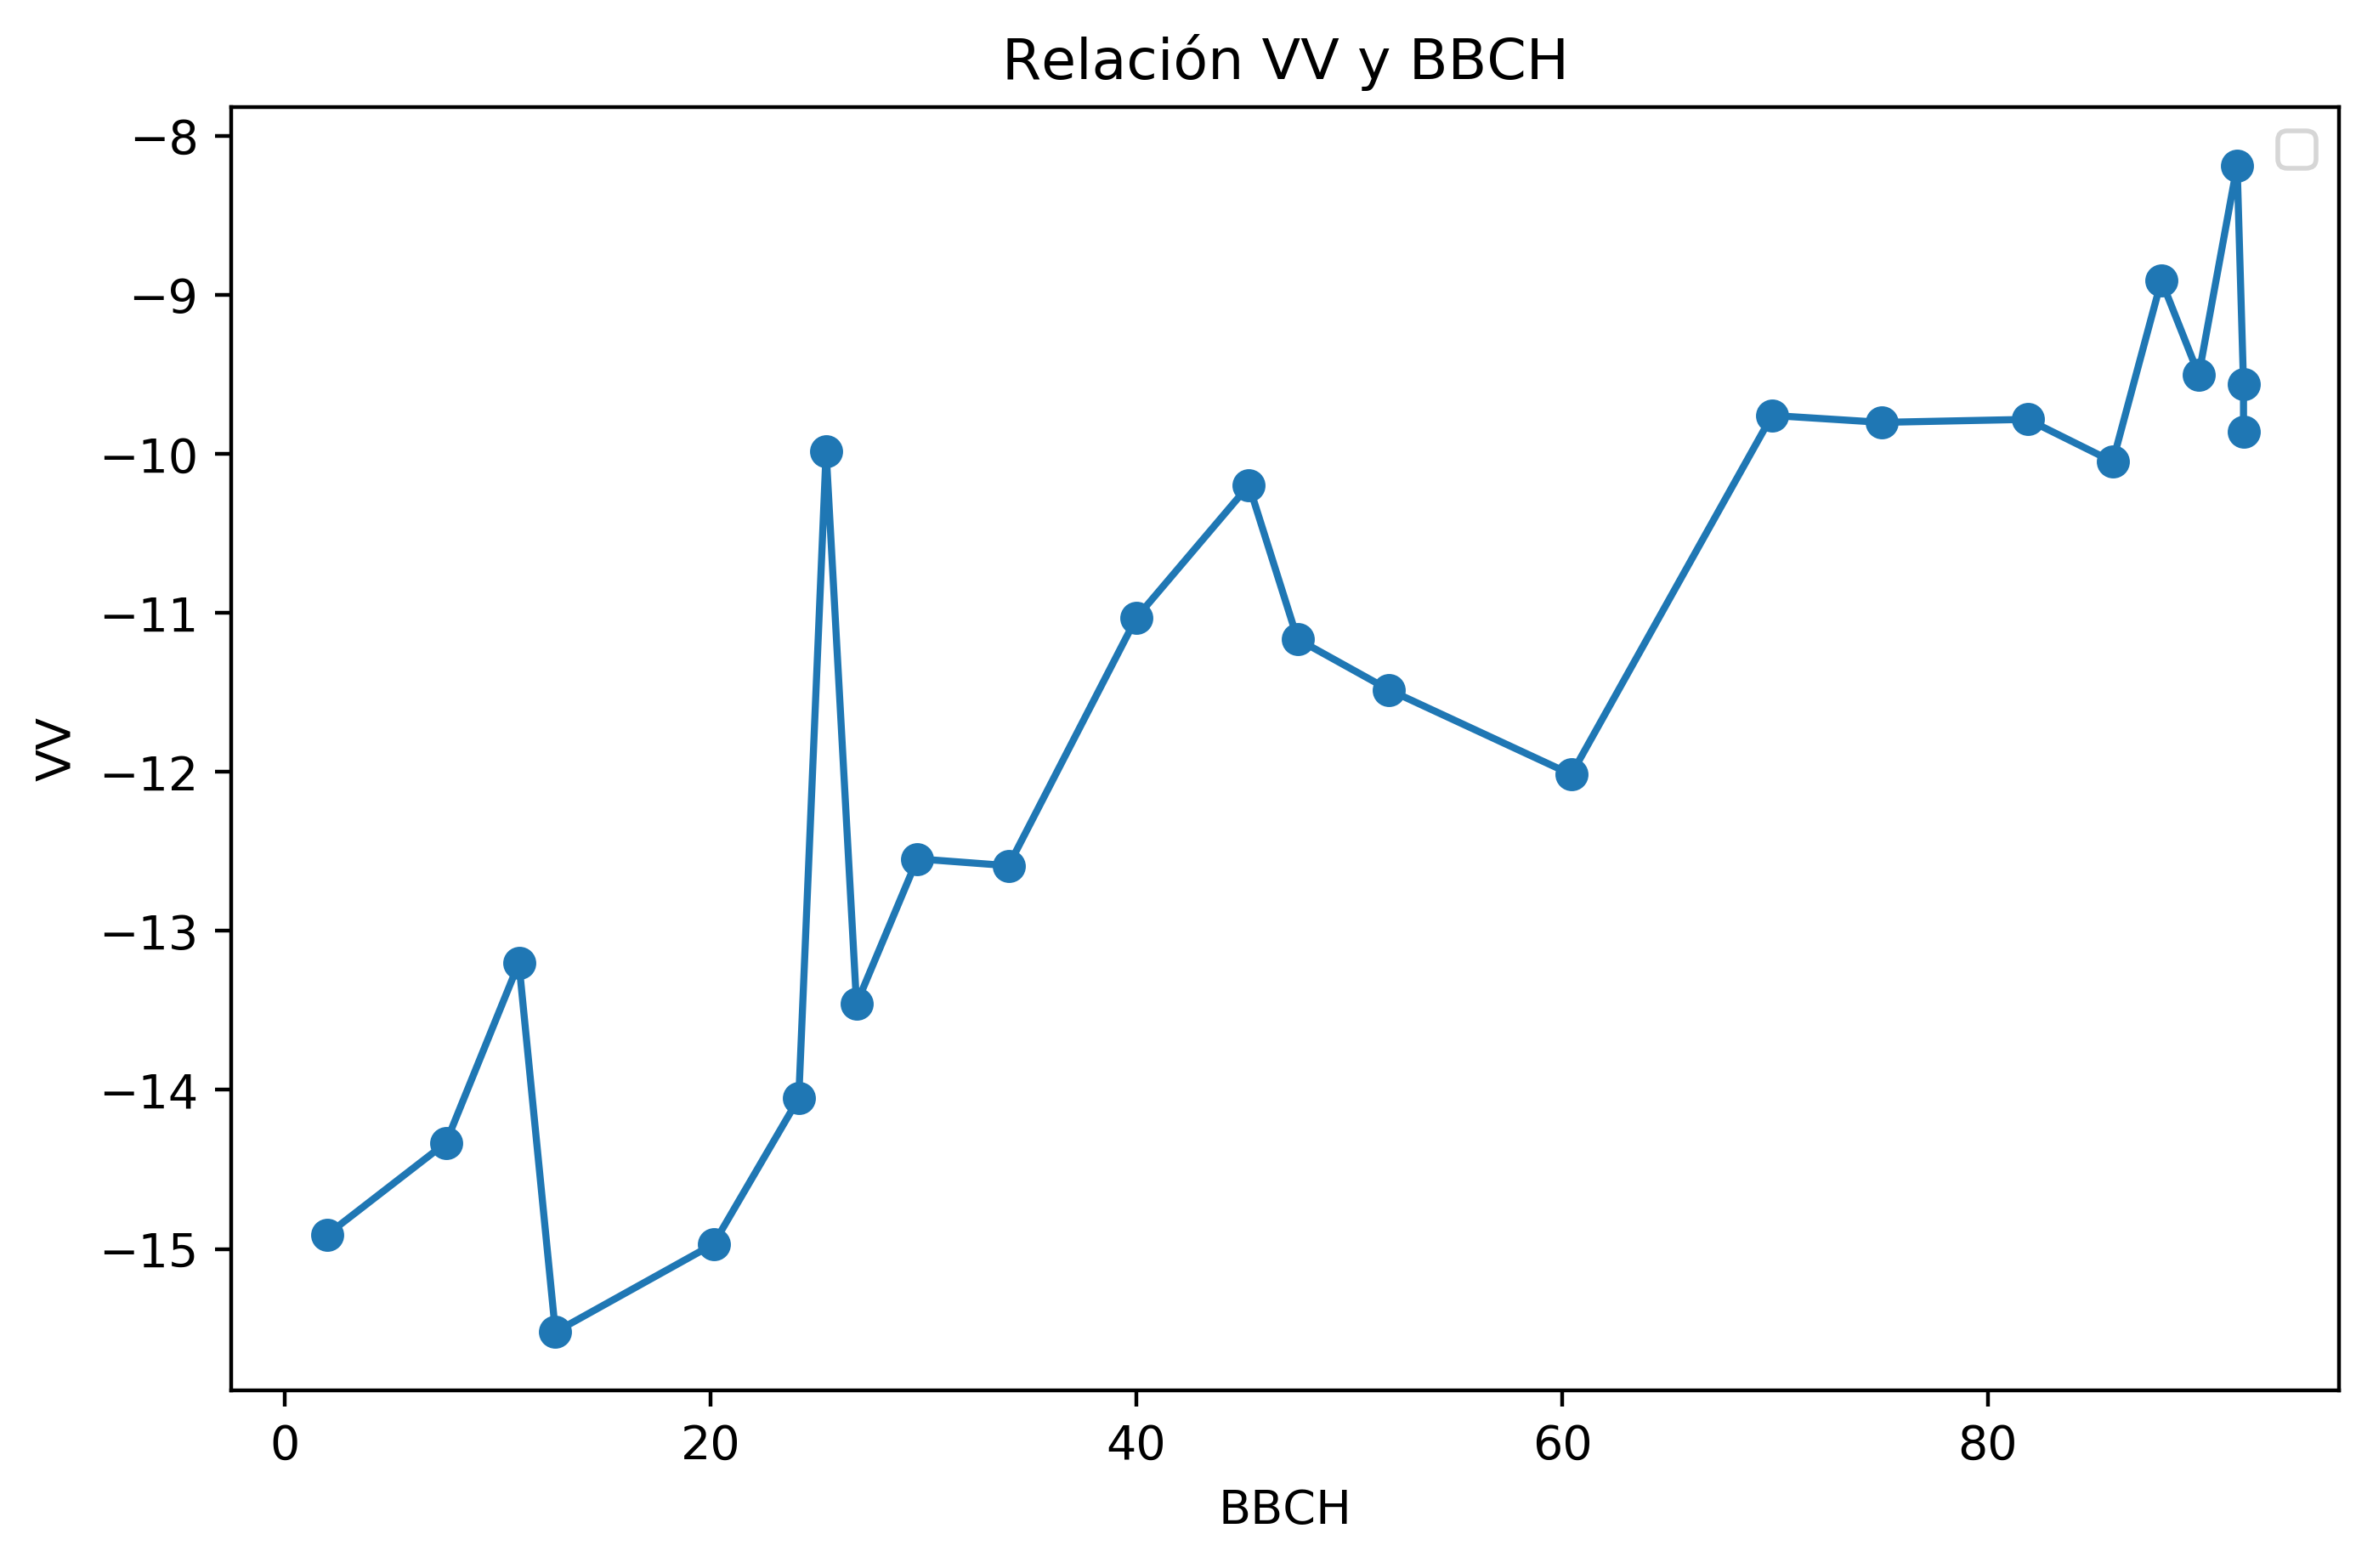
\includegraphics[width=\linewidth]{archivos/VV}
  \caption{Relación de la variable VV con respecto a la \gls{bbch}. \label{fig:VV}}
\end{subfigure}%
\begin{subfigure}{.45\textwidth}
  \centering
  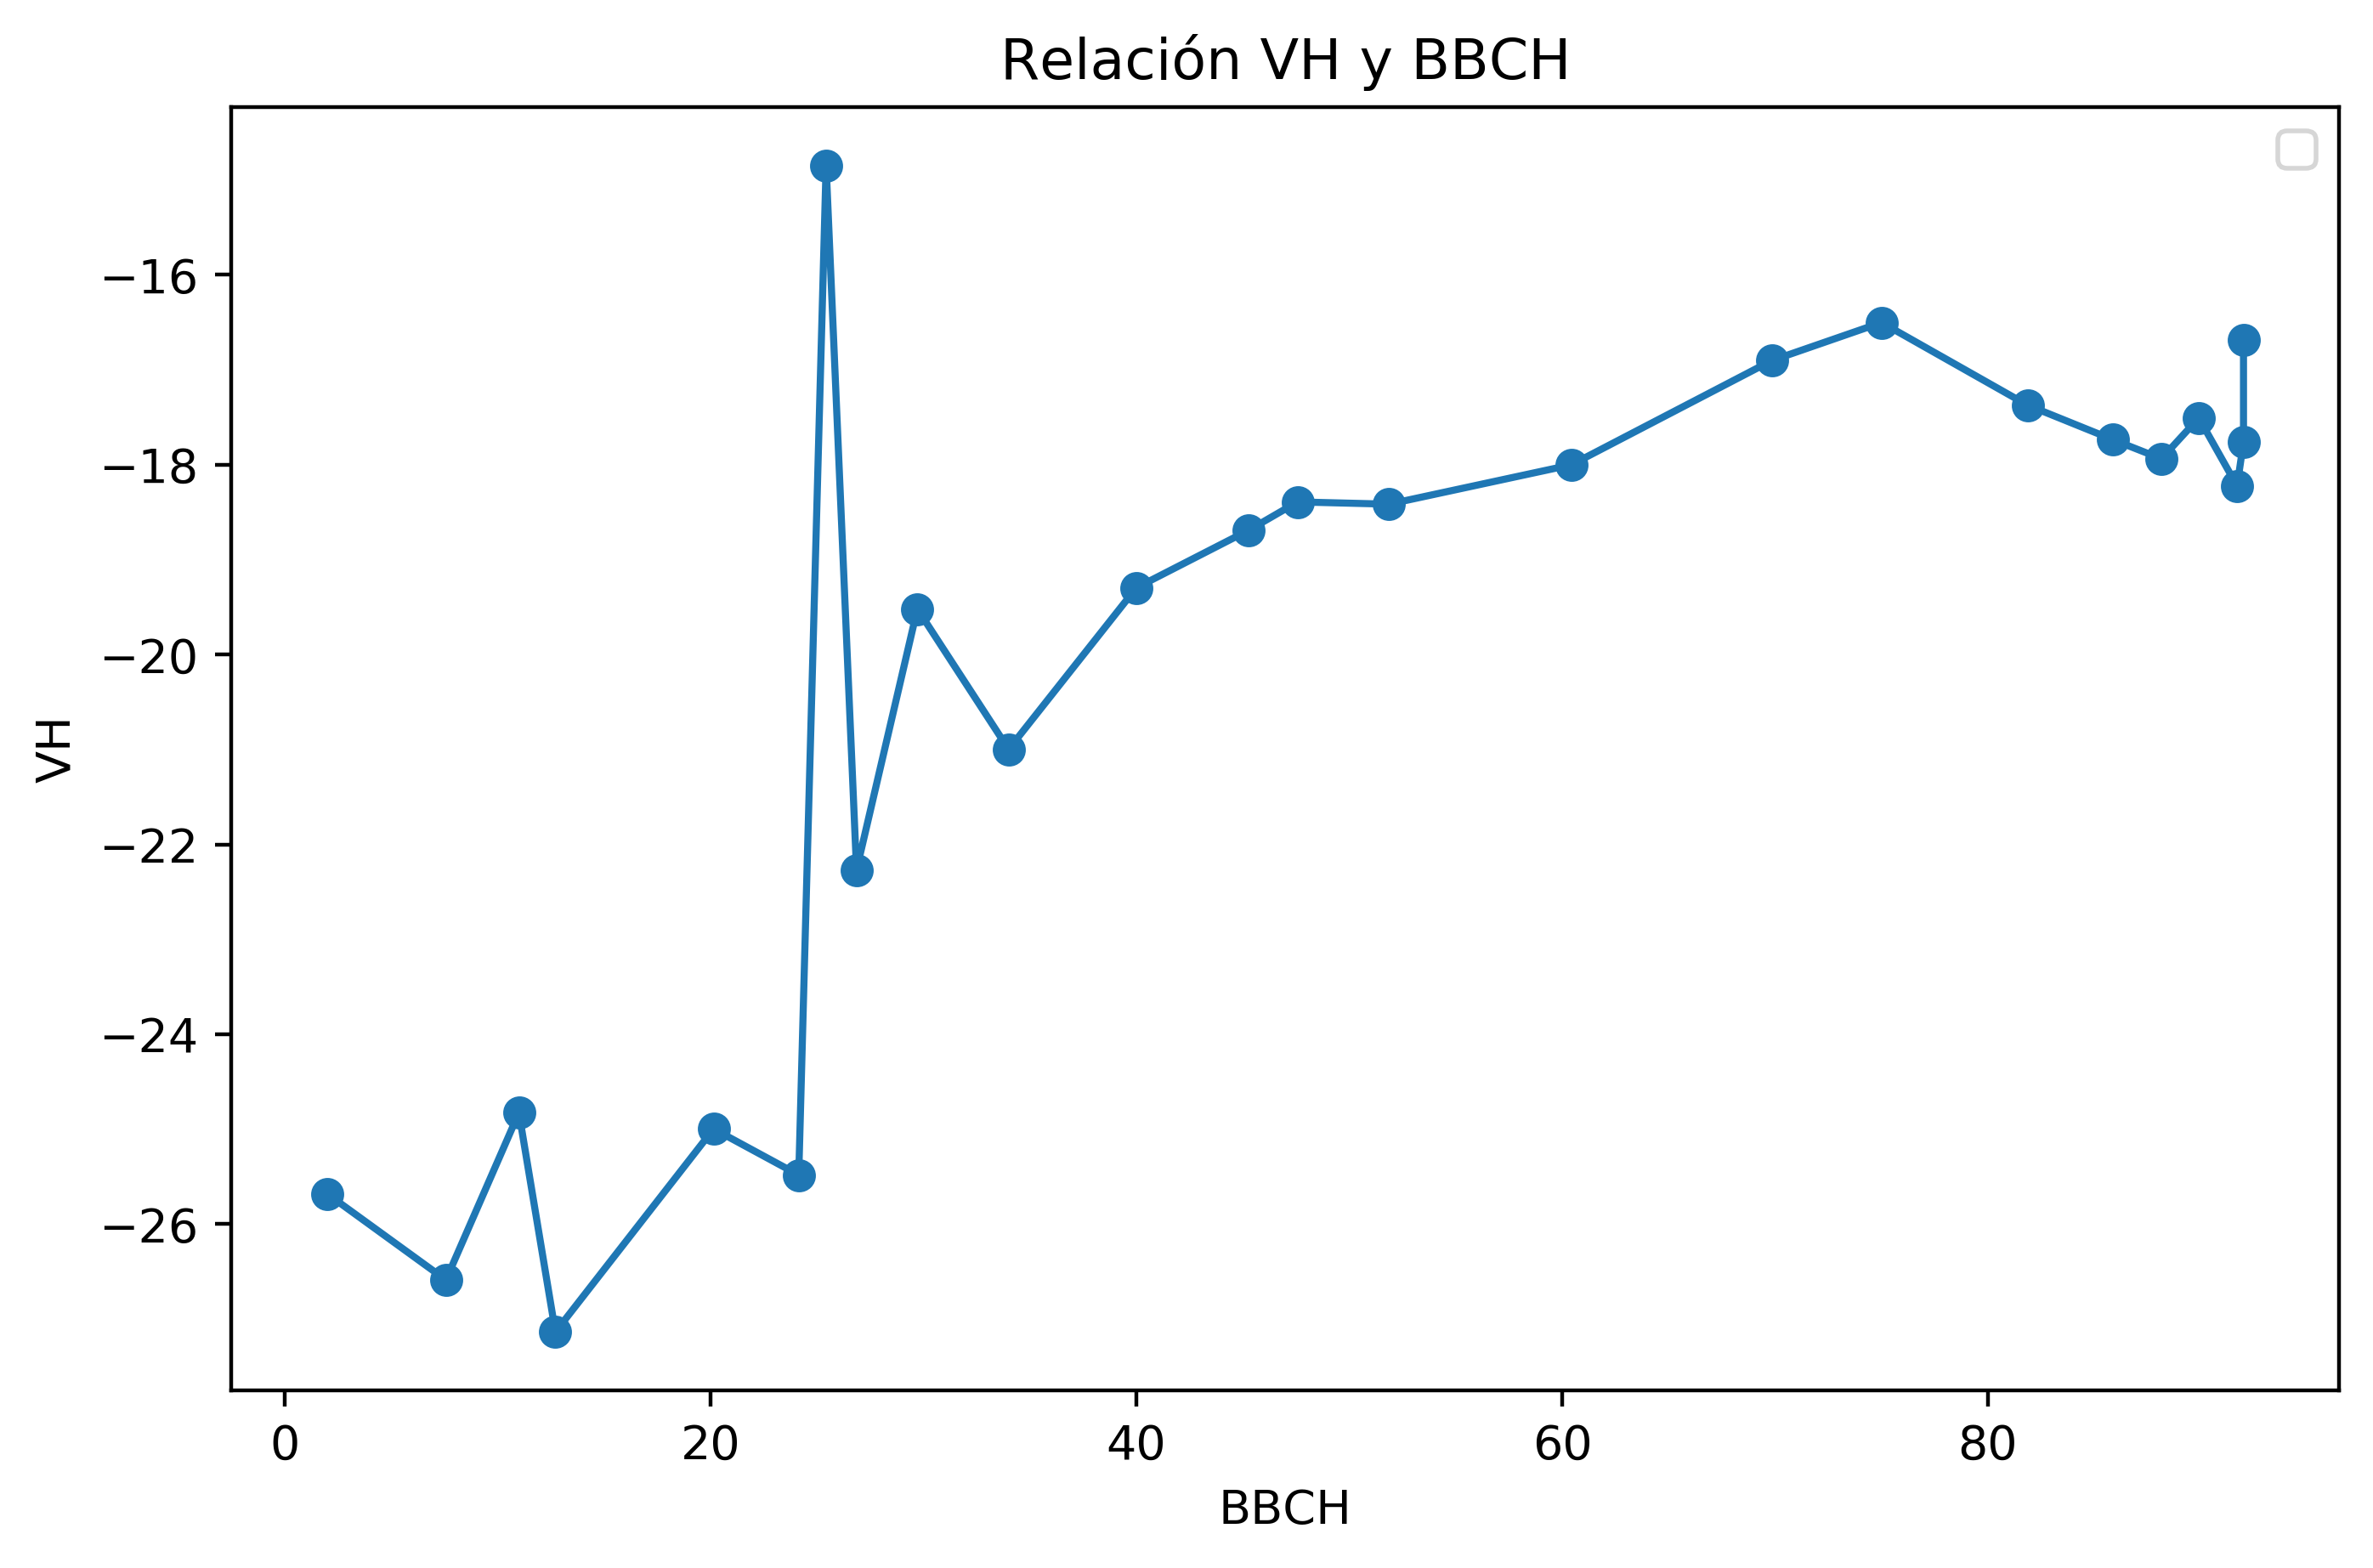
\includegraphics[width=\linewidth]{archivos/VH}
  \caption{Relación de la variable VH con respecto a la \gls{bbch}.\label{fig:VH}}
\end{subfigure}
\begin{subfigure}{.45\textwidth}
  \centering
  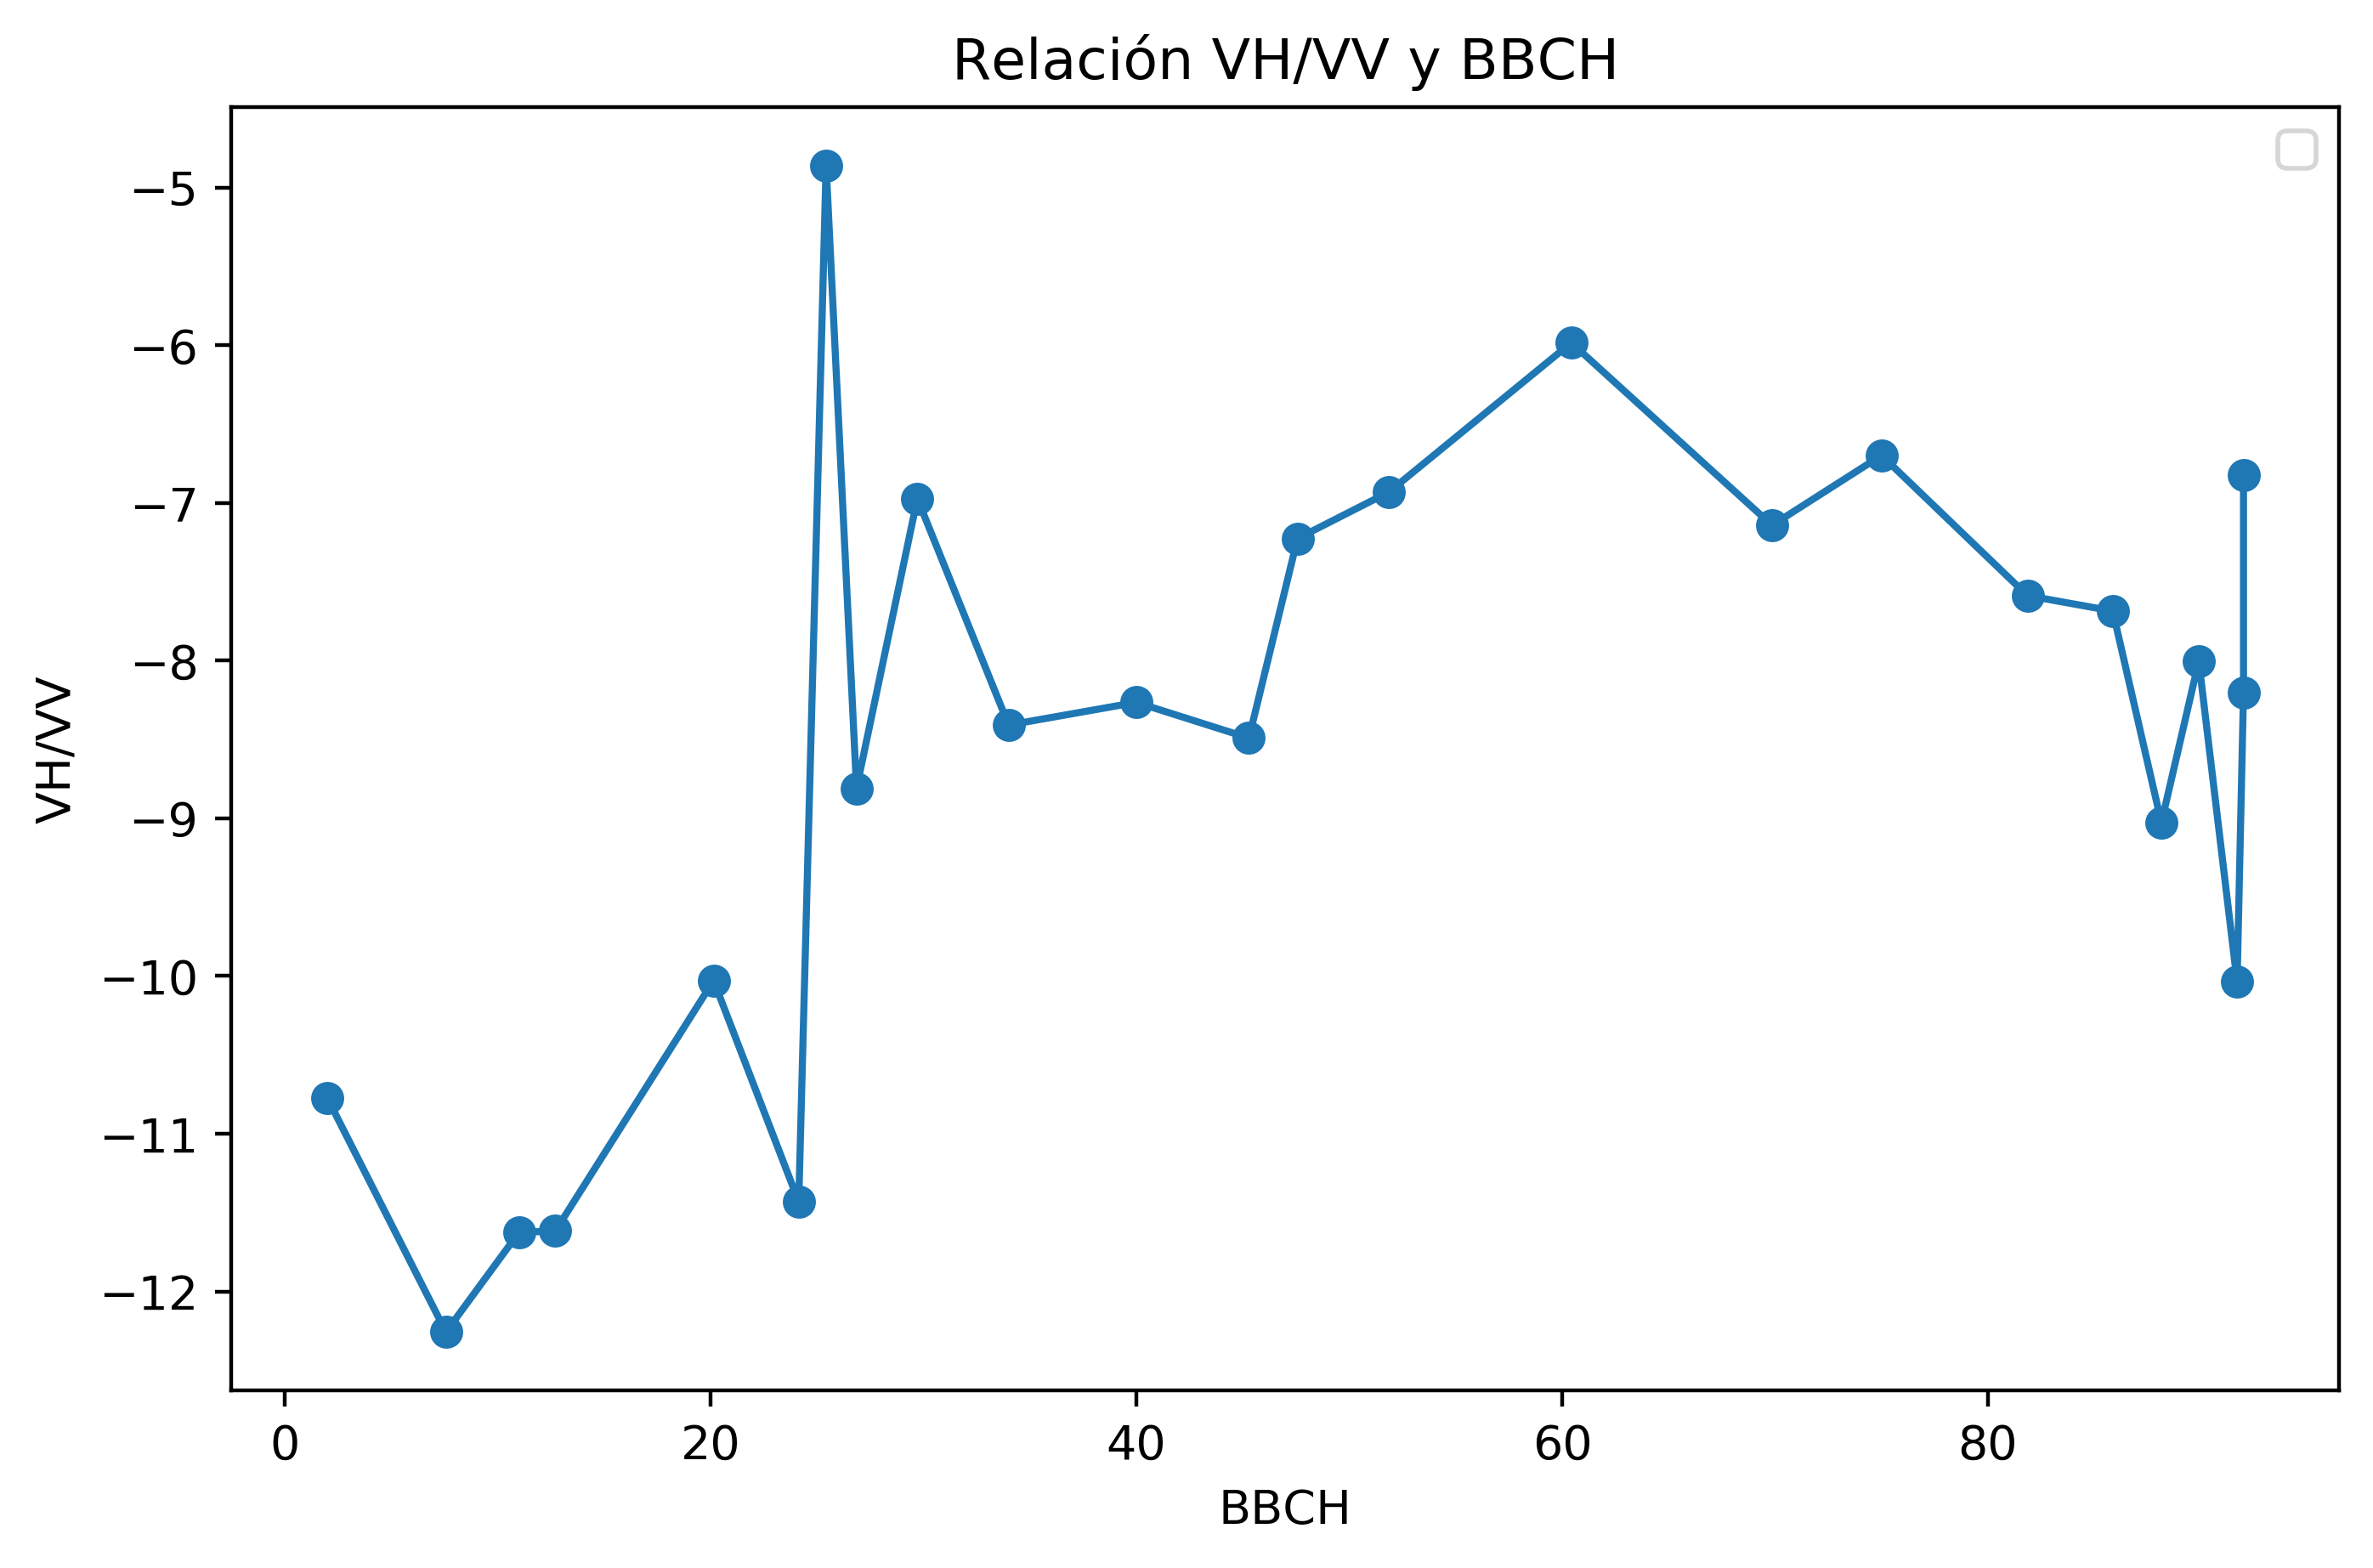
\includegraphics[width=\linewidth]{archivos/RATIO}
  \caption{Relación de la variable ratio VH/VV con respecto a la \gls{bbch}.\label{fig:RATIO}}
\end{subfigure}
\caption{Relación de las variables de datos de entrada al modelo con respecto a la \gls{bbch} \label{fig:rel_param}}
\end{figure}

%%%%%%%%%%%%%%%%%%%
%%%%%%%%%%%%%%%%%%%
\section{Método por píxeles} 
\subsection{Optimización}
\par La optimización de los datos de entrada para este método se realiza de igual manera que el anterior, coincidiendo los mejores resultados para todos los casos en el uso de un conjunto de 6 parcelas para entrenamiento y 1 para la evaluación y los datos de entrada, se reducen a los tres principales (VV, VH y ratio) a nivel de pixel, por lo que las desviaciones estándar no son necesarias. En cuanto a la optimización del regresor, se utiliza también la relación entre el número de árboles para un modelo y el coeficiente de determinación, presentado en la imagen de ejemplo \ref{fig:opt_pixl} con el caso de salida \gls{bbch}. En ella, se puede ver que una vez alcanzado cierto nivel de coeficiente, la mejora de este en relación al aumento del número de árboles no es significativa con respecto al costo computacional y a la complejidad del sistema que se crea. 
\begin{figure}[h]
    \centering
    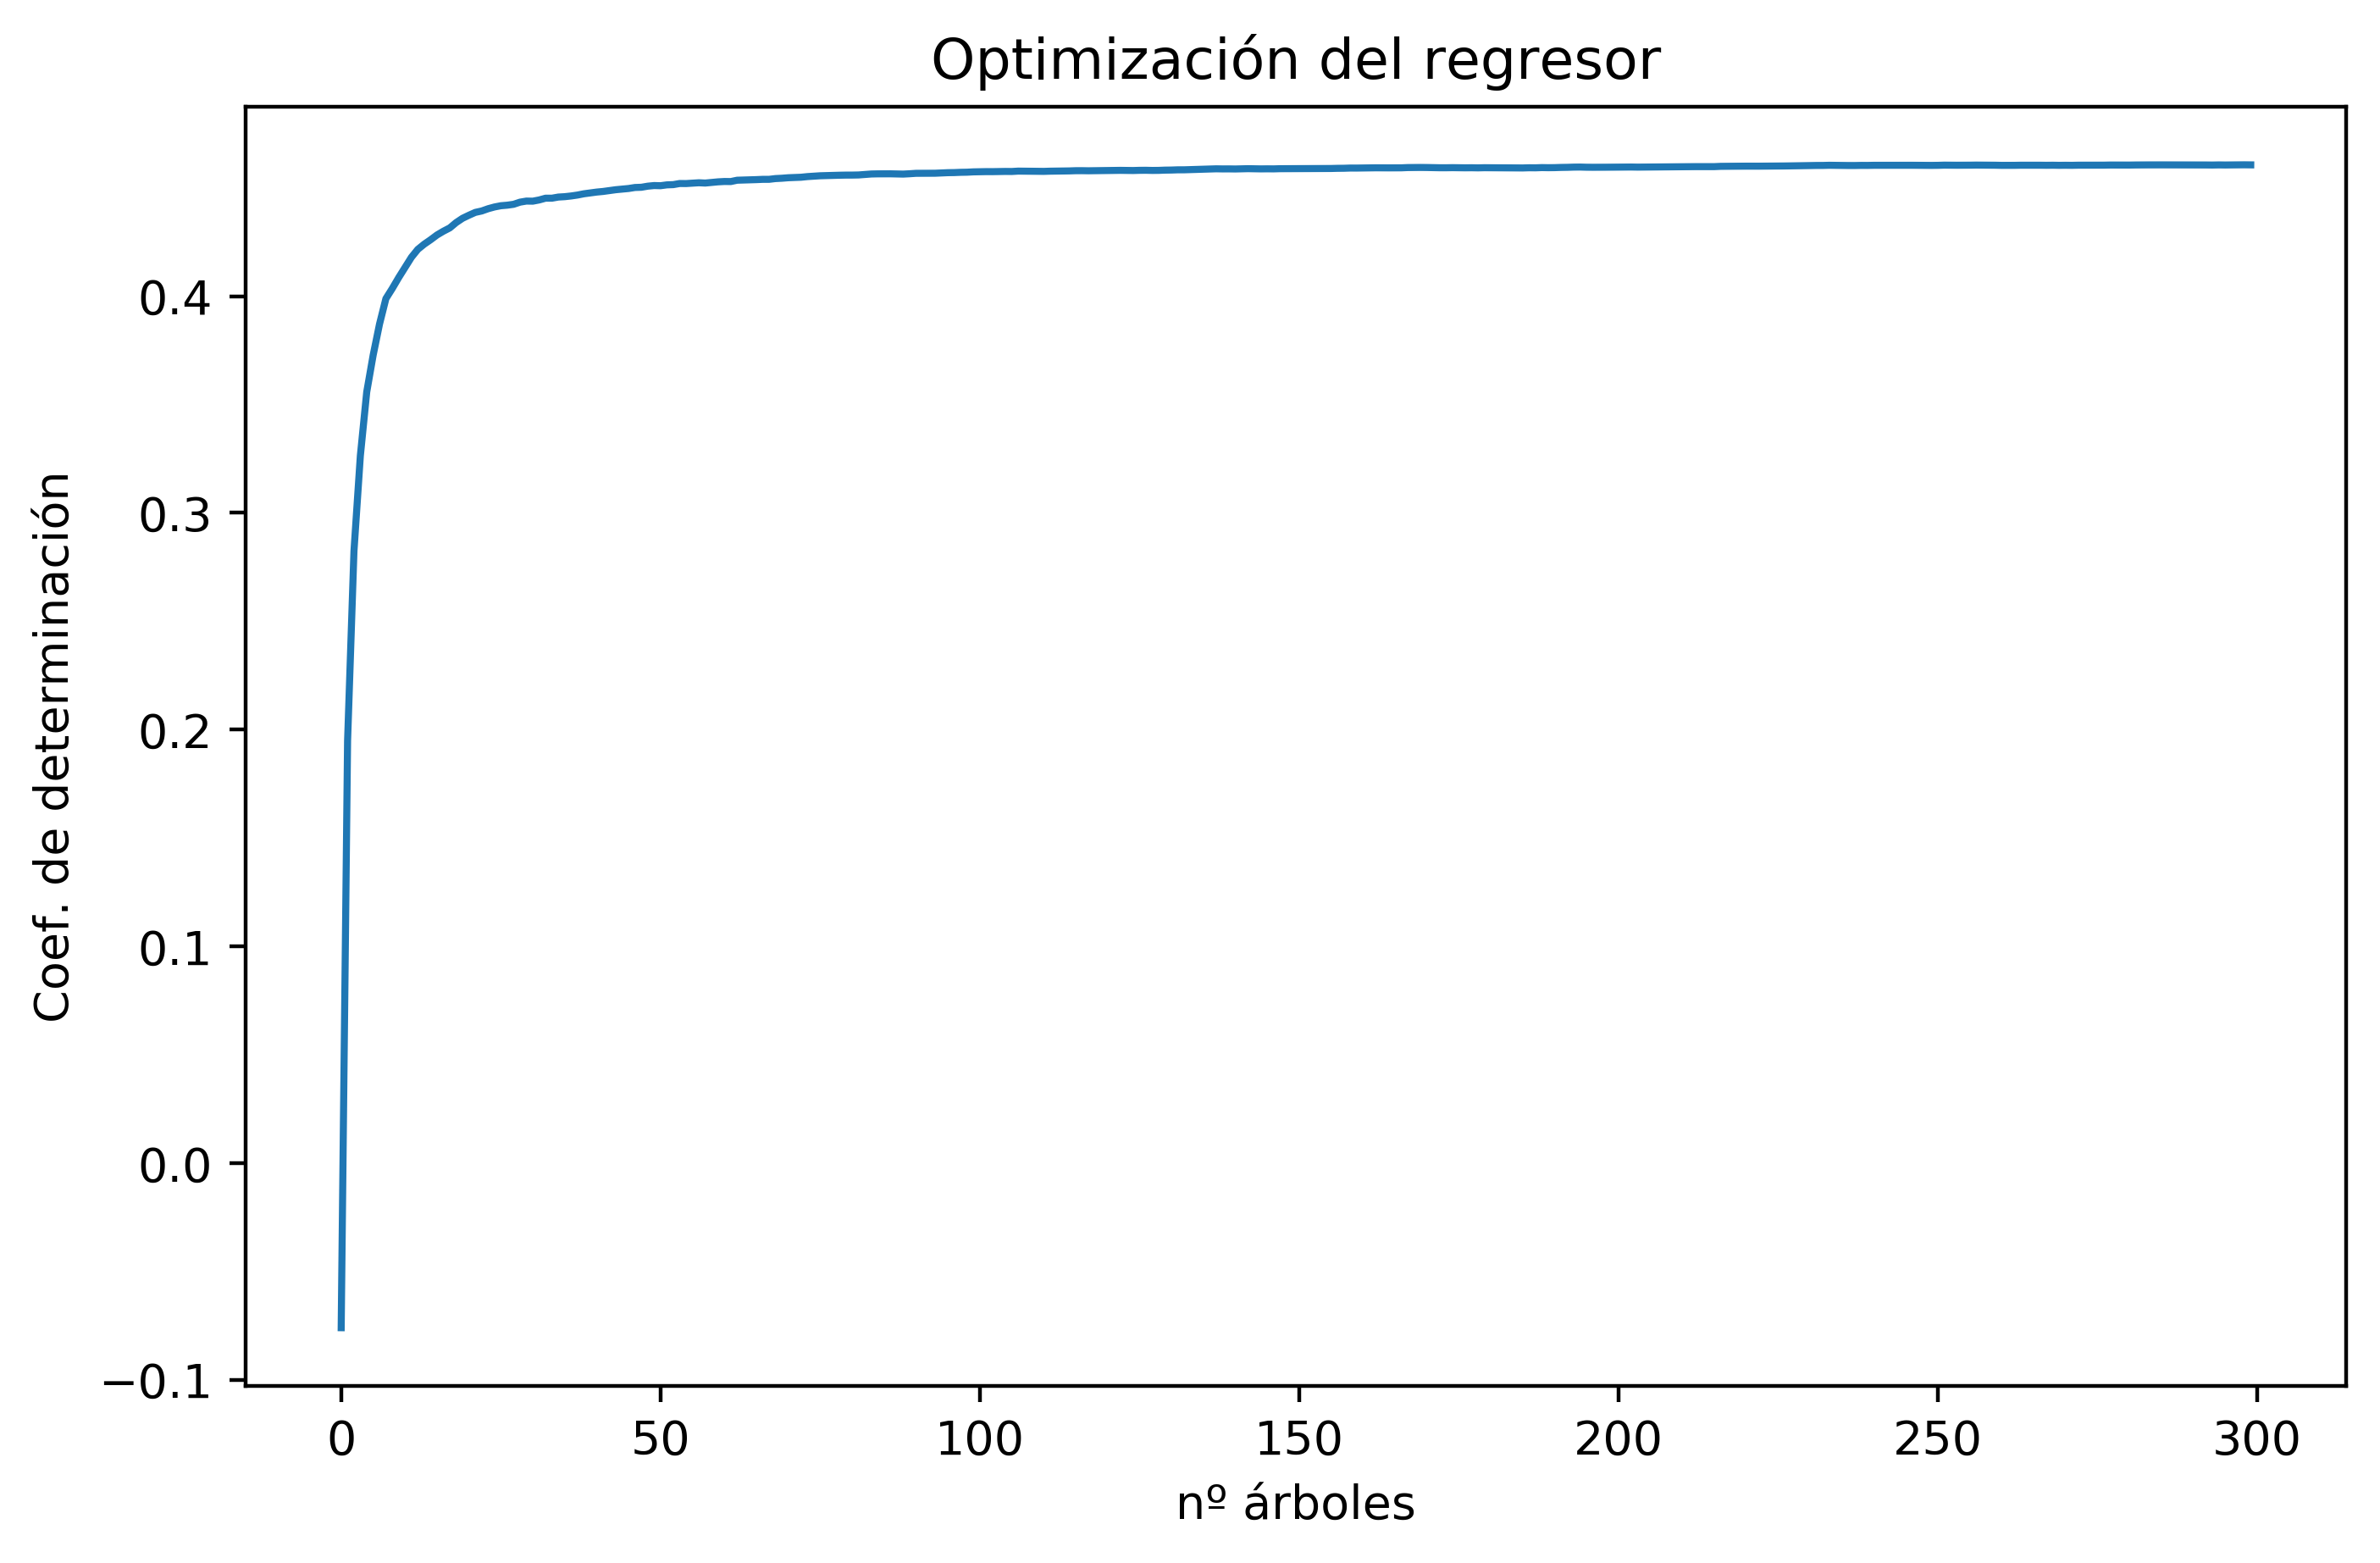
\includegraphics[height=9cm]{archivos/tfg/Pixel/opt_tree_bbch_pixel} 
    \caption{Optimización del número de árboles para \gls{rfr} en el modelo de salida \gls{bbch}}
    \label{fig:opt_pixl}
\end{figure}

\par Finalmente, los parámetros utilizados en este método para cada caso se presentan en la tabla \ref{tab:opt_pixl}, donde se pueden ver: la parcela utilizada para el periodo de test del modelo; siendo el resto de parcelas utilizadas en el entrenamiento, y el número de árboles óptimo para \gls{rfr}, de acuerdo con la evolución del coeficiente de determinación para cada caso.

\begin{table}[h]
\centering
\begin{tabular}{l|ccc}
                  & \gls{bbch}     & Altura   & \gls{bbch}\&Altura \\ \hline
Parcela de test   & `Mínima' & `Mínima' & `Mínima'     \\
Número de árboles & 46       & 48       & 47          
\end{tabular}
\caption{Parámetros de optimización de entrada y modelo \label{tab:opt_pixl}}
\end{table}

\par Como se puede observar, los 3 casos coinciden en el set de parcelas de entrenamiento y test con el que se obtienen mejores resultados. Probablemente esto se debe a anomalías en el desarrollo de algunas parcelas, las cuales, si se toman como set de test, el modelo no las habría podido tener en cuenta en el aprendizaje y el error en la predicción sería mayor. Los 3 casos de este método constan de un número óptimo de árboles muy similares, con una diferencia de 1 y 2 con respecto al caso menor. Cabe destacar que el aumento de complejidad, aunque escaso, en el modelo de salida de la altura, como ocurre para el método anterior. Además, tanto para la metodología por píxeles como por parcelas, se obtiene un número óptimo de árboles para el caso de 2 salidas intermedio a los óptimos para las mismas salidas en modelos independientes. Esto se debe a una compensación en la estimación de ambas variables, para que una variable sea óptima sin que su mejora sea a costa de la otra se llega a un valor intermedio en el que ninguna de las salidas está totalmente optimizada pero tienen el mejor resultado del sistema compartido completo. 


\subsection{Salidas del modelo}
\subsubsection{Salidas de función de densidad de probabilidad}
Como se ha mencionado en la metodología anterior, las salidas útiles de este trabajo son las \gls{pdf}. En las figuras \ref{fig:p_pdf_b} (modelo de salida \gls{bbch}), \ref{fig:p_pdf_h} (modelo de salida altura) y \ref{fig:p_pdf_bh} (modelo de ambas salidas) se puede apreciar cómo son algunas de estas salidas en esta metodología, siendo ejemplos extraídos a partir de los mismos datos para los 3 casos estudiados. 
\\
% Dos figuras sueltas debajo de otra
\begin{figure}[h]
\centering
\begin{subfigure}{0.6\textwidth}
	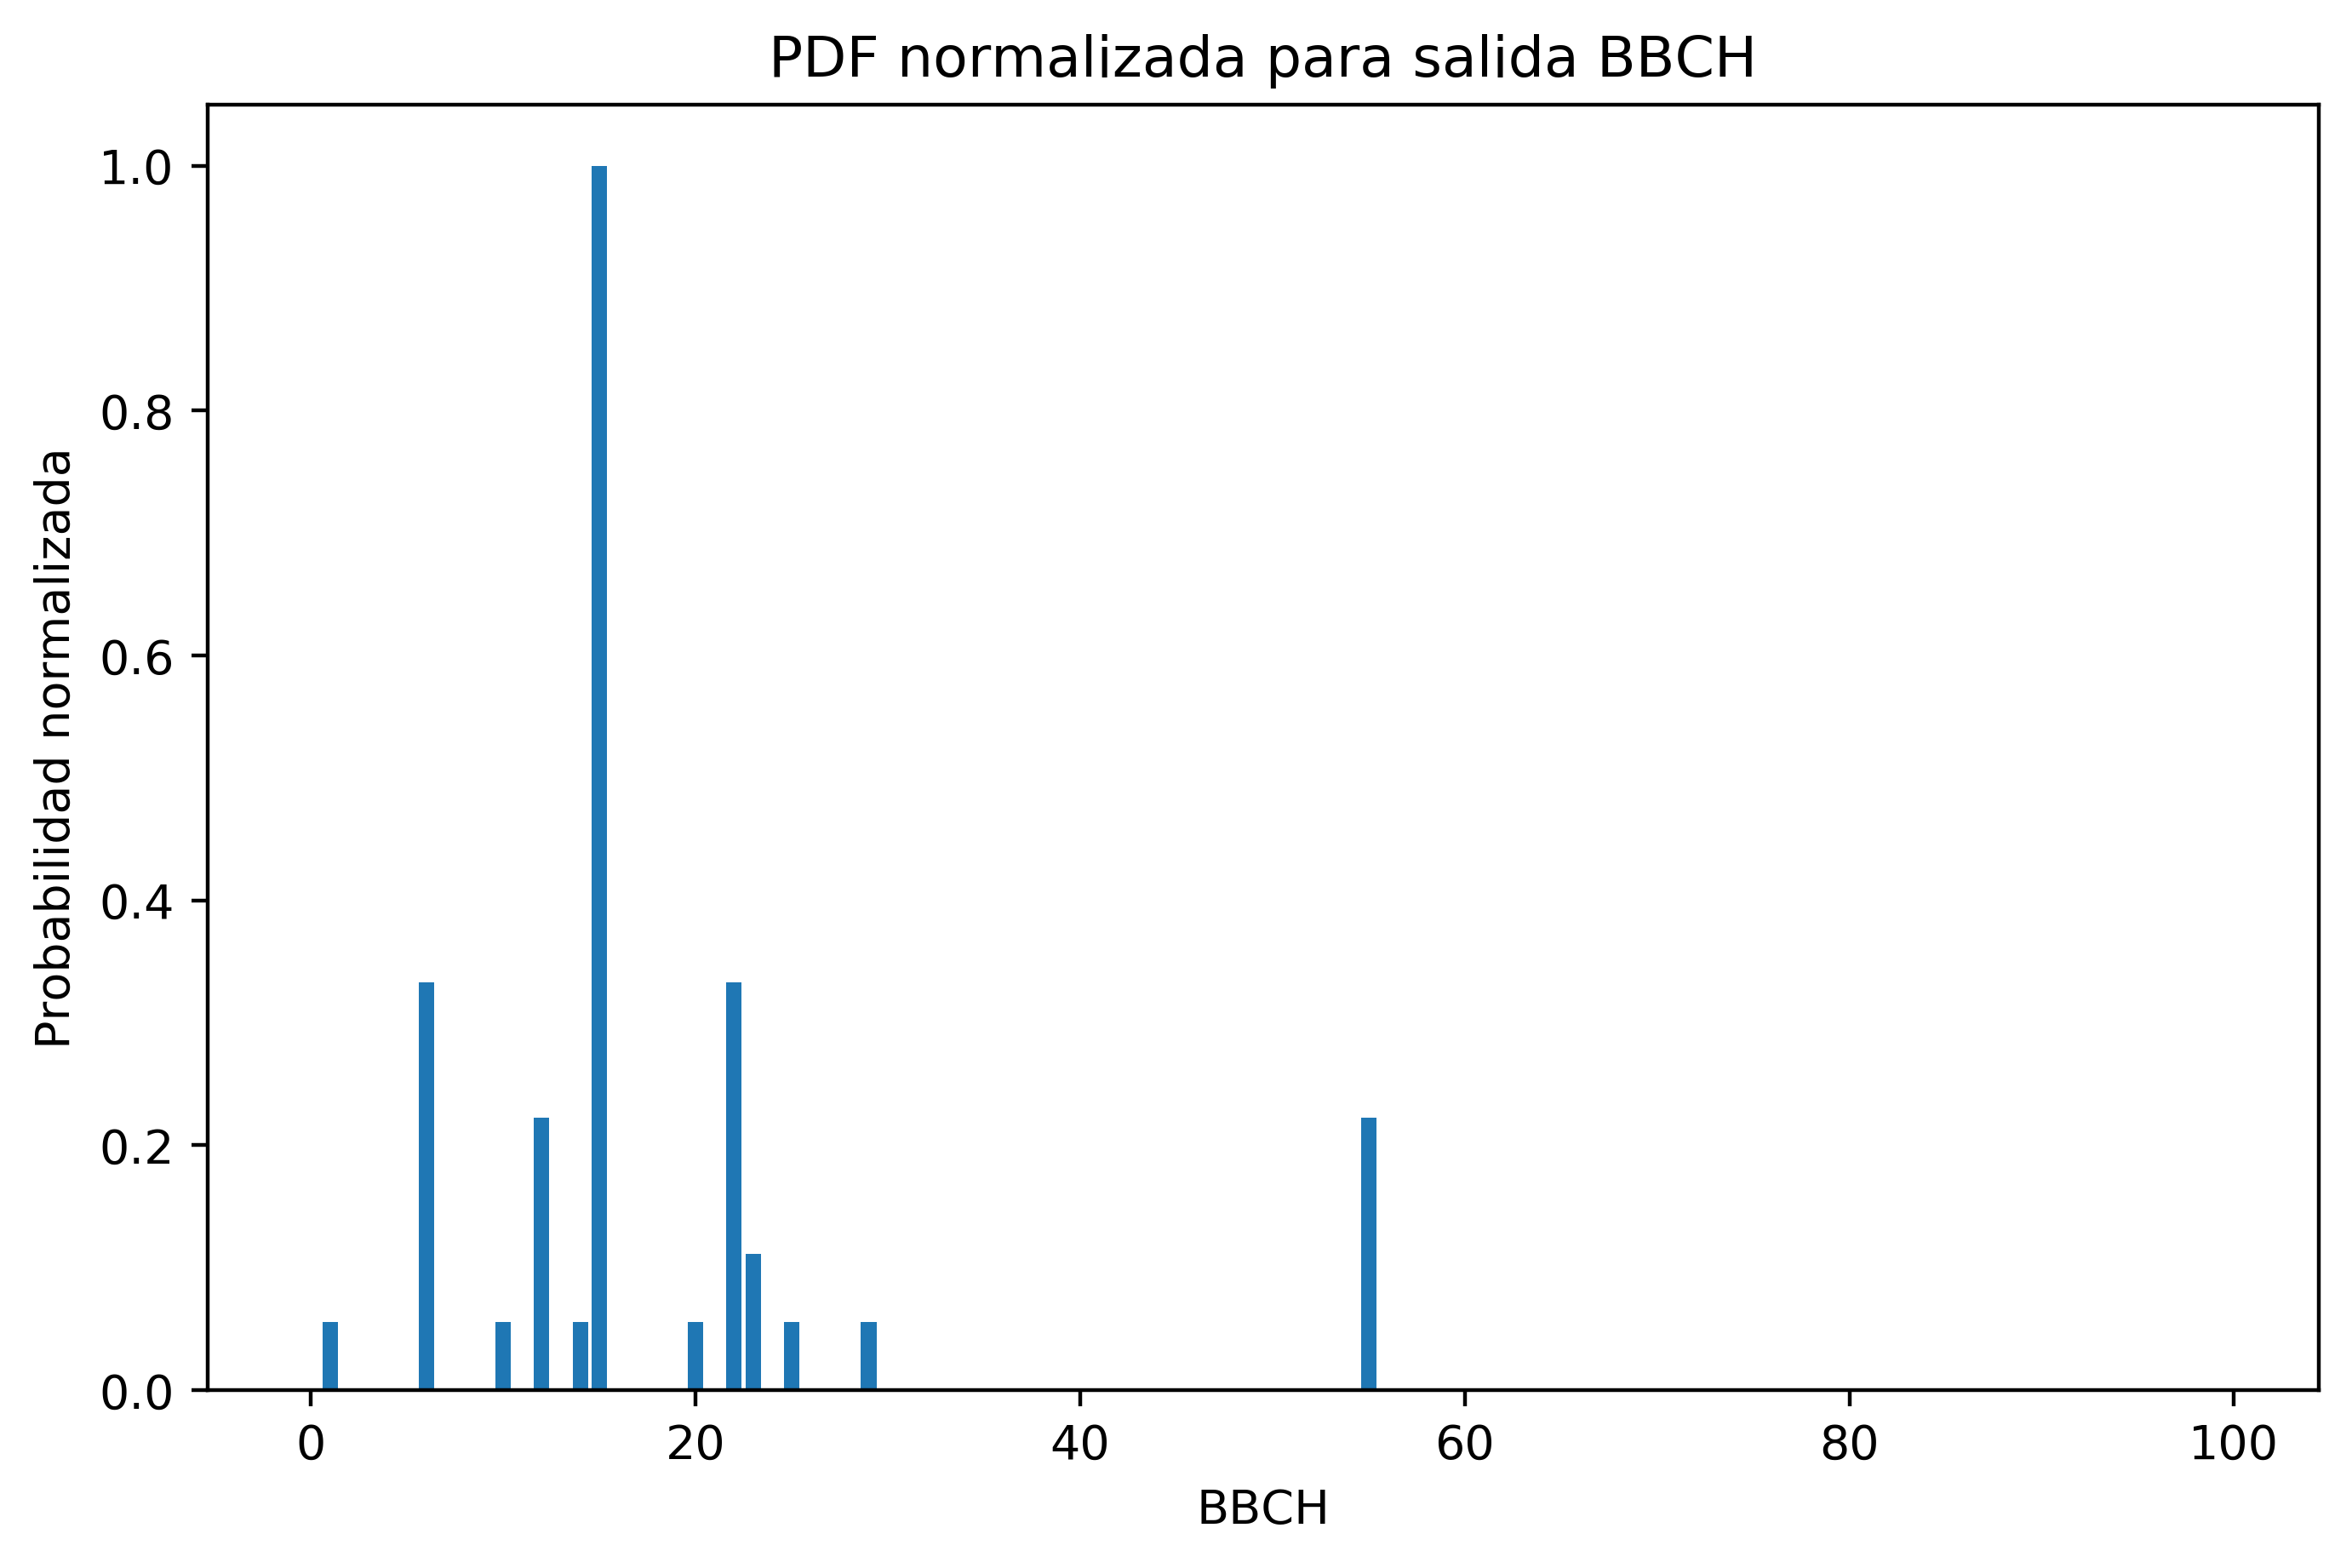
\includegraphics[width=\linewidth]{archivos/tfg/Pixel/BBCH_PDF}
	\caption{Ejemplo de salida \gls{pdf} normalizada del 			modelo para estimación de \gls{bbch}.\label{fig:p_pdf_b}}
\end{subfigure}
\begin{subfigure}{0.6\textwidth}
	\centering
	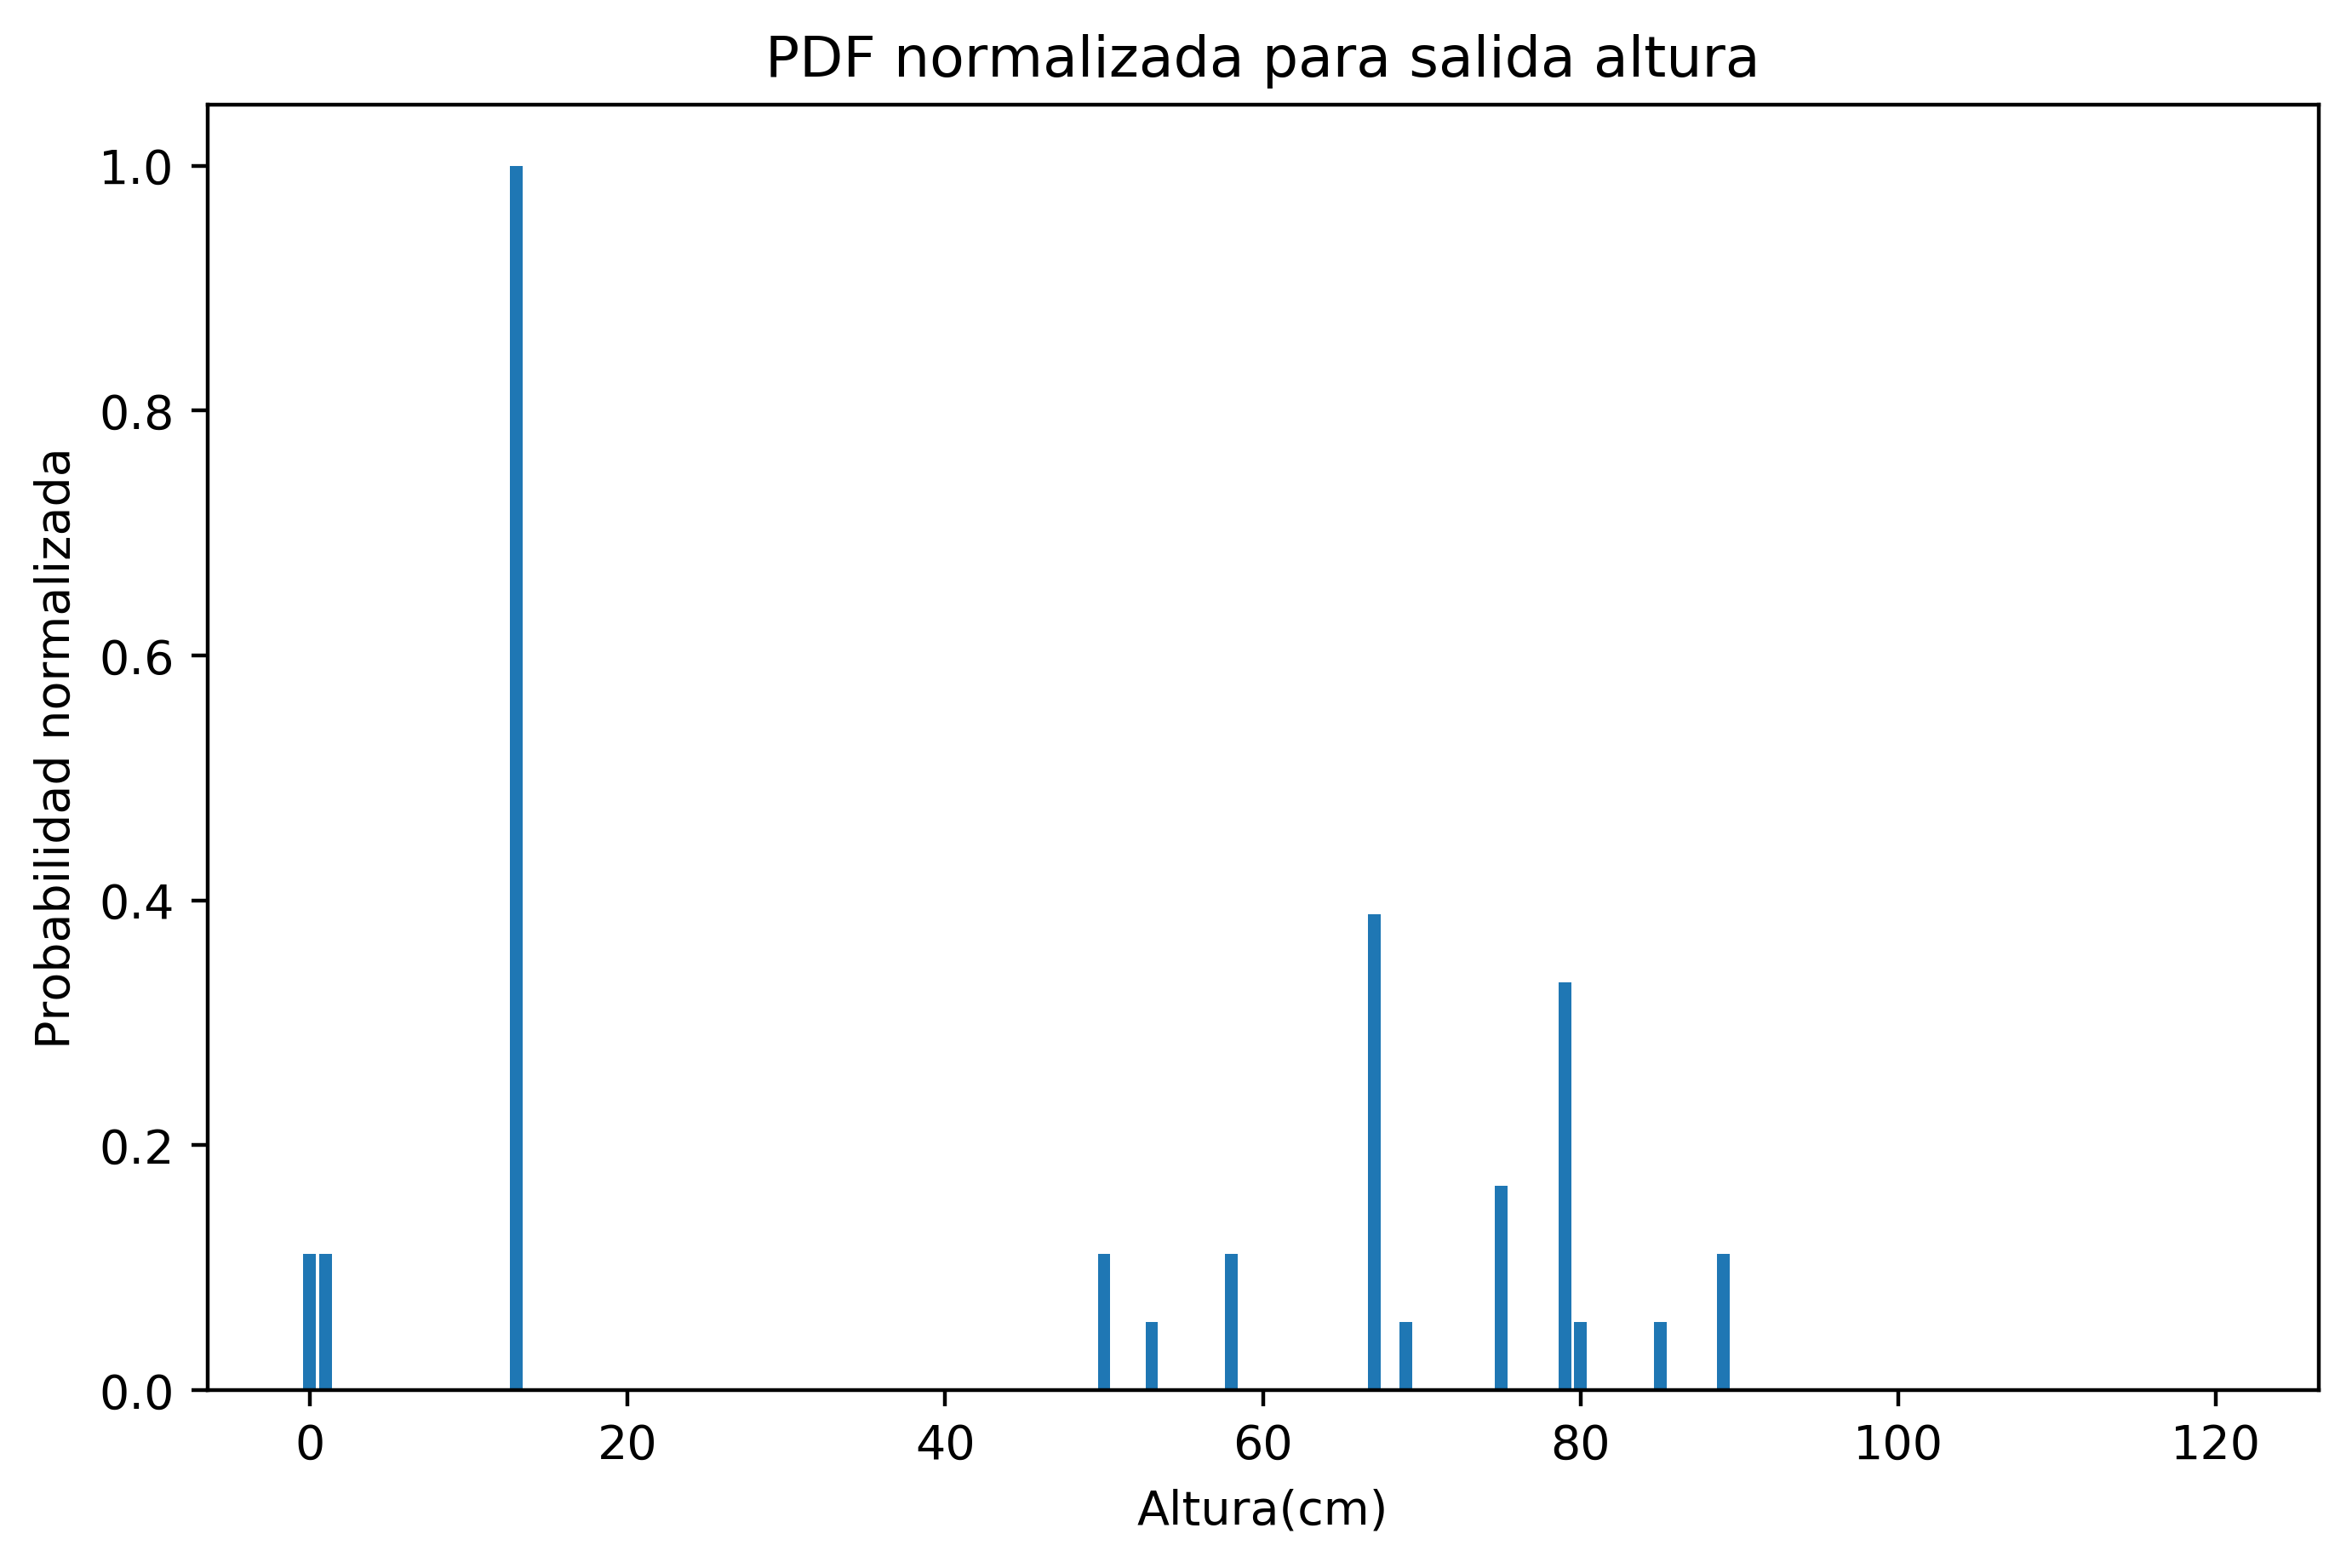
\includegraphics[width=\linewidth]{archivos/tfg/Pixel/H_PDF}
	\caption{Ejemplo de salida \gls{pdf} normalizada del 			modelo para estimación de la altura. \label{fig:p_pdf_h}}
	\end{subfigure}
	\caption{Ejemplo de salida \gls{pdf} normalizada los 			modelos para estimación de las variables independientes. \label{fig:p_pdf}}
\end{figure}

\par Estas representaciones tienen las mismas características mencionadas anteriormente: están normalizadas con respecto a la salida con mayor probabilidad, destaca una salida predominante pero no se excluyen el resto a la hora de integrarse con el modelo de predicción temporal. 
\\
\par Las figuras \ref{fig:p_pdf} y \ref{fig:p_pdf_bh} han sido generadas con los mismos datos de entrada, es decir, los mismos datos de satélite en la misma parcela y fecha, por lo que las salidas para los modelos generados de estimación de \gls{bbch} (Figura \ref{fig:p_pdf_b}) y altura (Figura \ref{fig:p_pdf_h}) como modelos independientes se pueden comparar con las salidas del modelo de estimación de ambas (Figura \ref{fig:p_pdf_bh}). La principal diferencia que se vuelve a encontrar entre los mismos tipos de datos de salida para cada modelo es que, las salidas individuales presentan una estimación principal con una diferencia de probabilidad mayor con respecto al resto que las estimaciones del modelo de doble salida. El rango para cada salida es bastante más amplio y disperso para el modelo de doble salida, esto junto a la disminución de diferencias con las demás estimaciones, indica que ese sistema es menos preciso y estable. En este modelo de dos salidas no se ve una clara optimización para una de ellas con respecto a la otra,  ya que además ambas tiene valores muy cercanos al sistema individual.

% Una figura con dos imágenes
\begin{figure}[H]
\centering
\begin{subfigure}{0.6\textwidth}
  \centering
  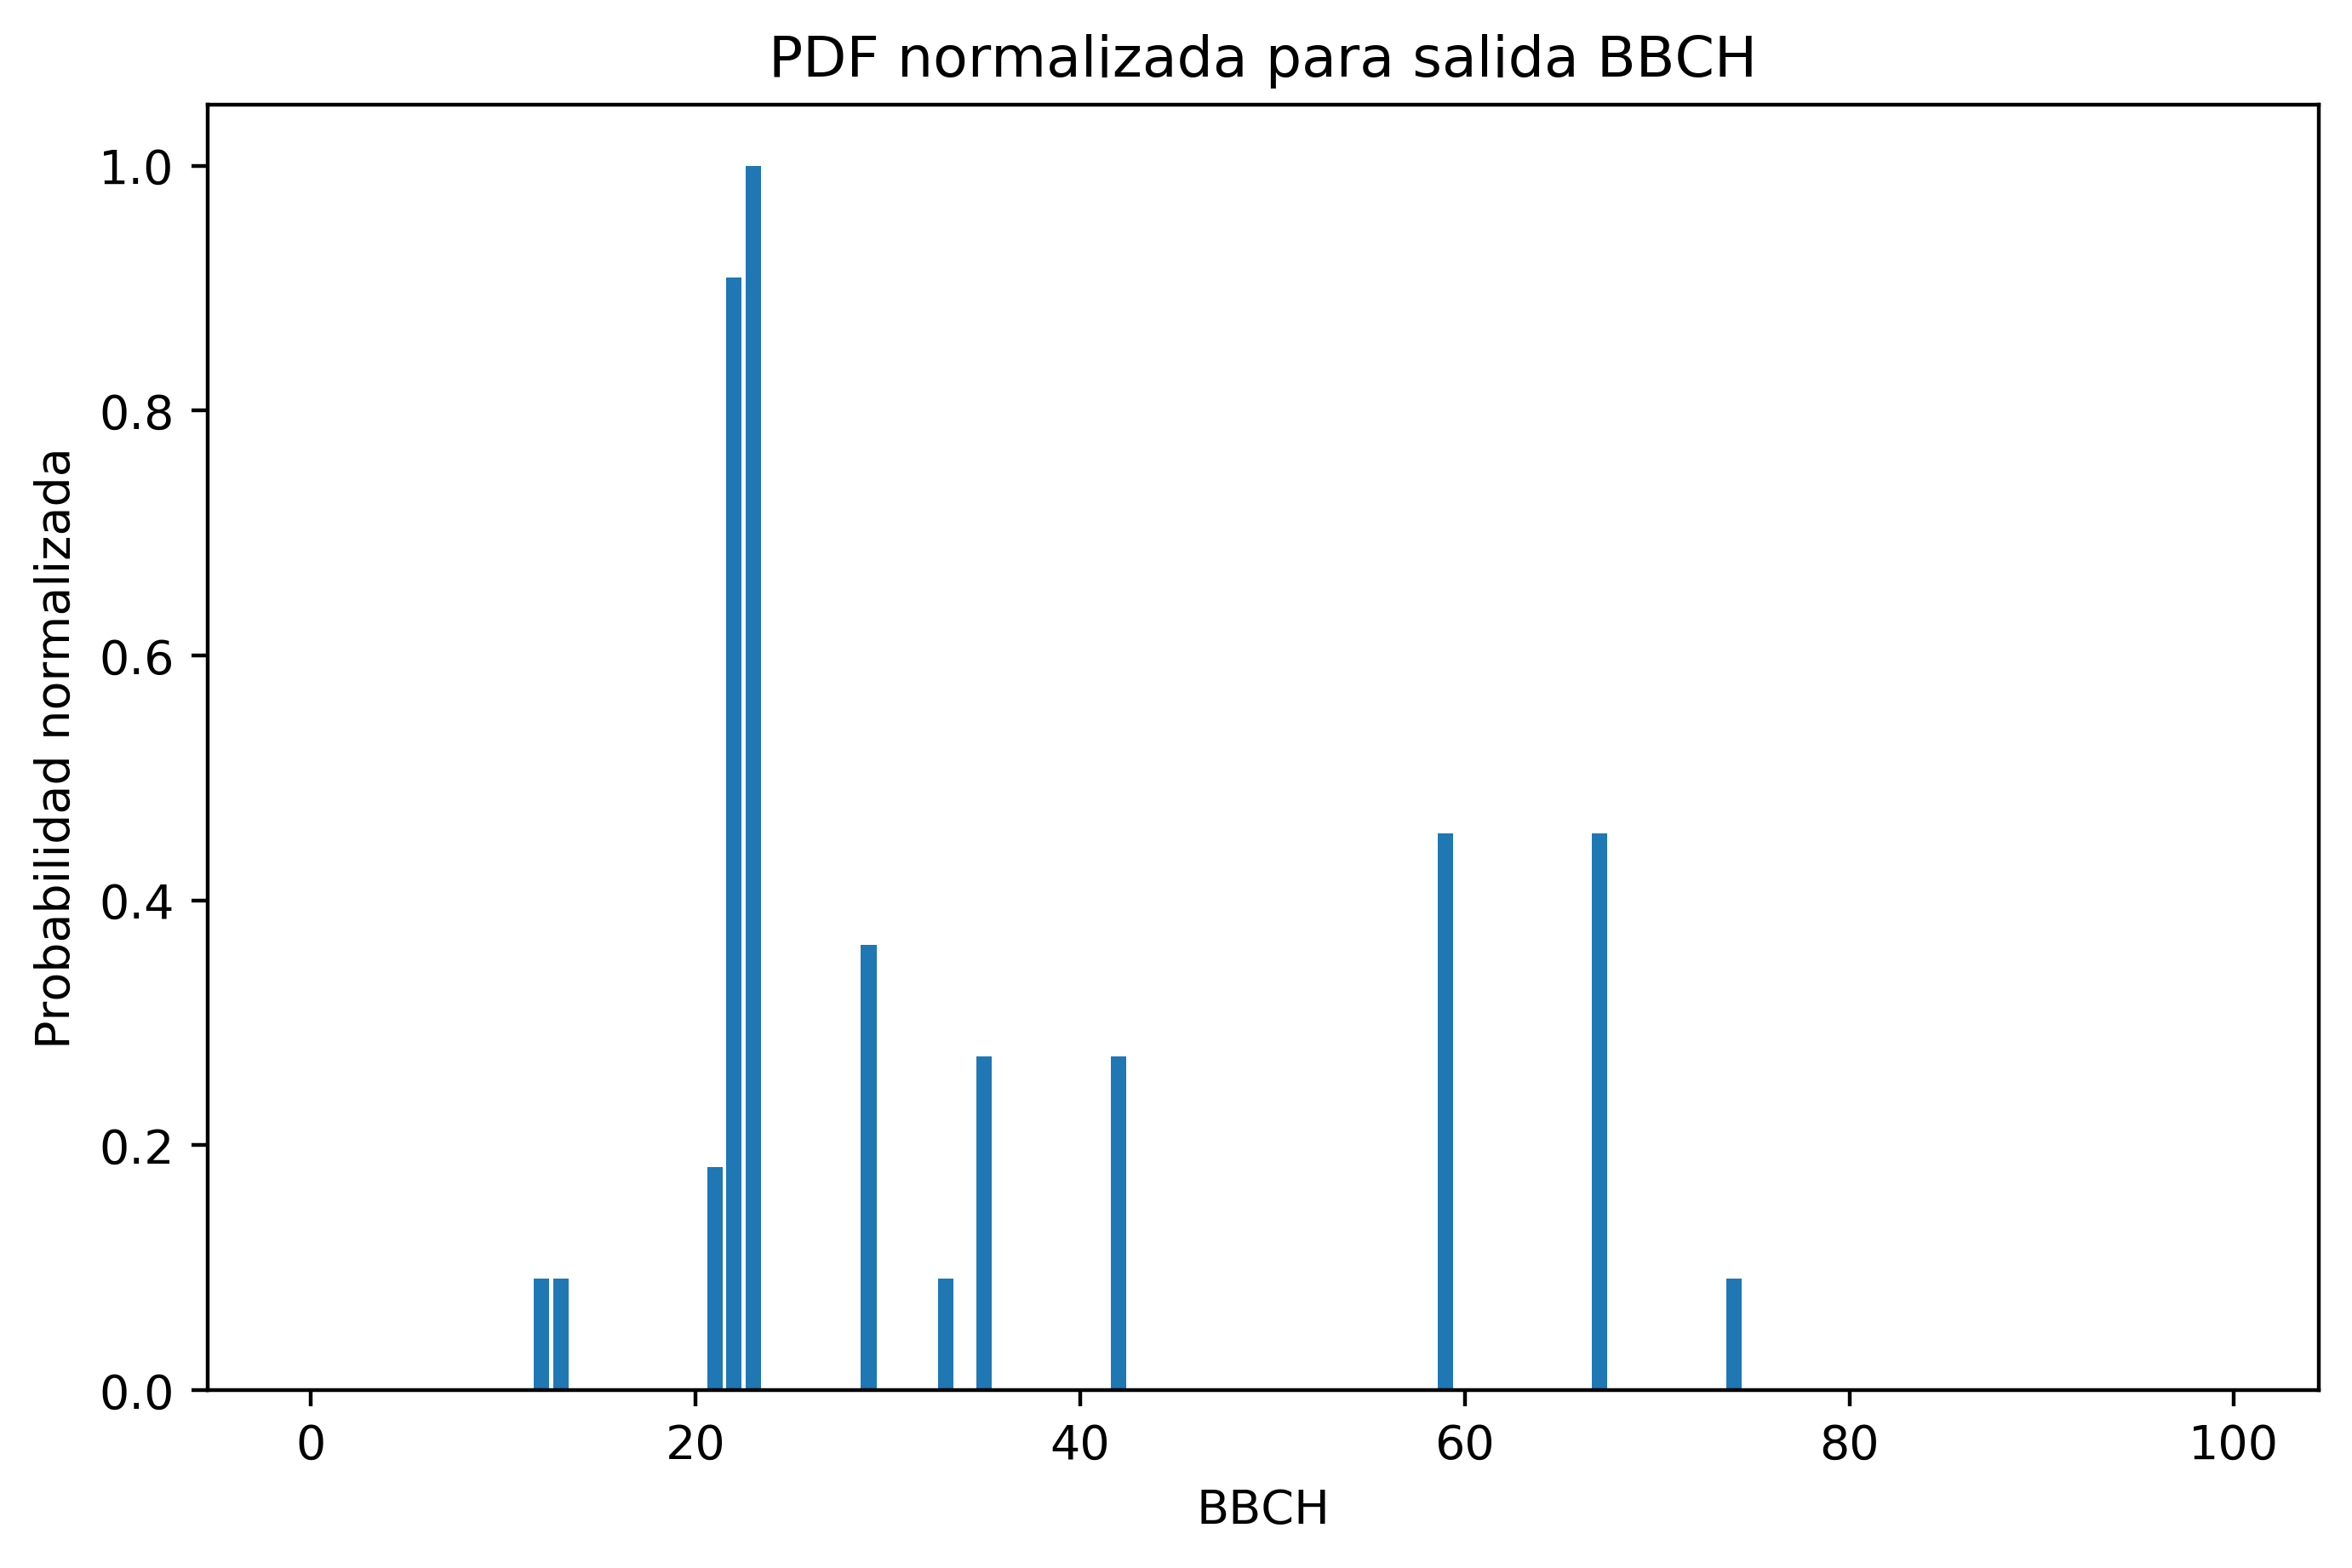
\includegraphics[width=0.95\linewidth]{archivos/tfg/Pixel/BBCHH_PDF_BBCH}
  \caption{Ejemplo del modelo de doble salida: \gls{pdf} estimación de \gls{bbch}\label{fig:p_sub1}}
\end{subfigure}
\begin{subfigure}{0.6\textwidth}
  \centering
  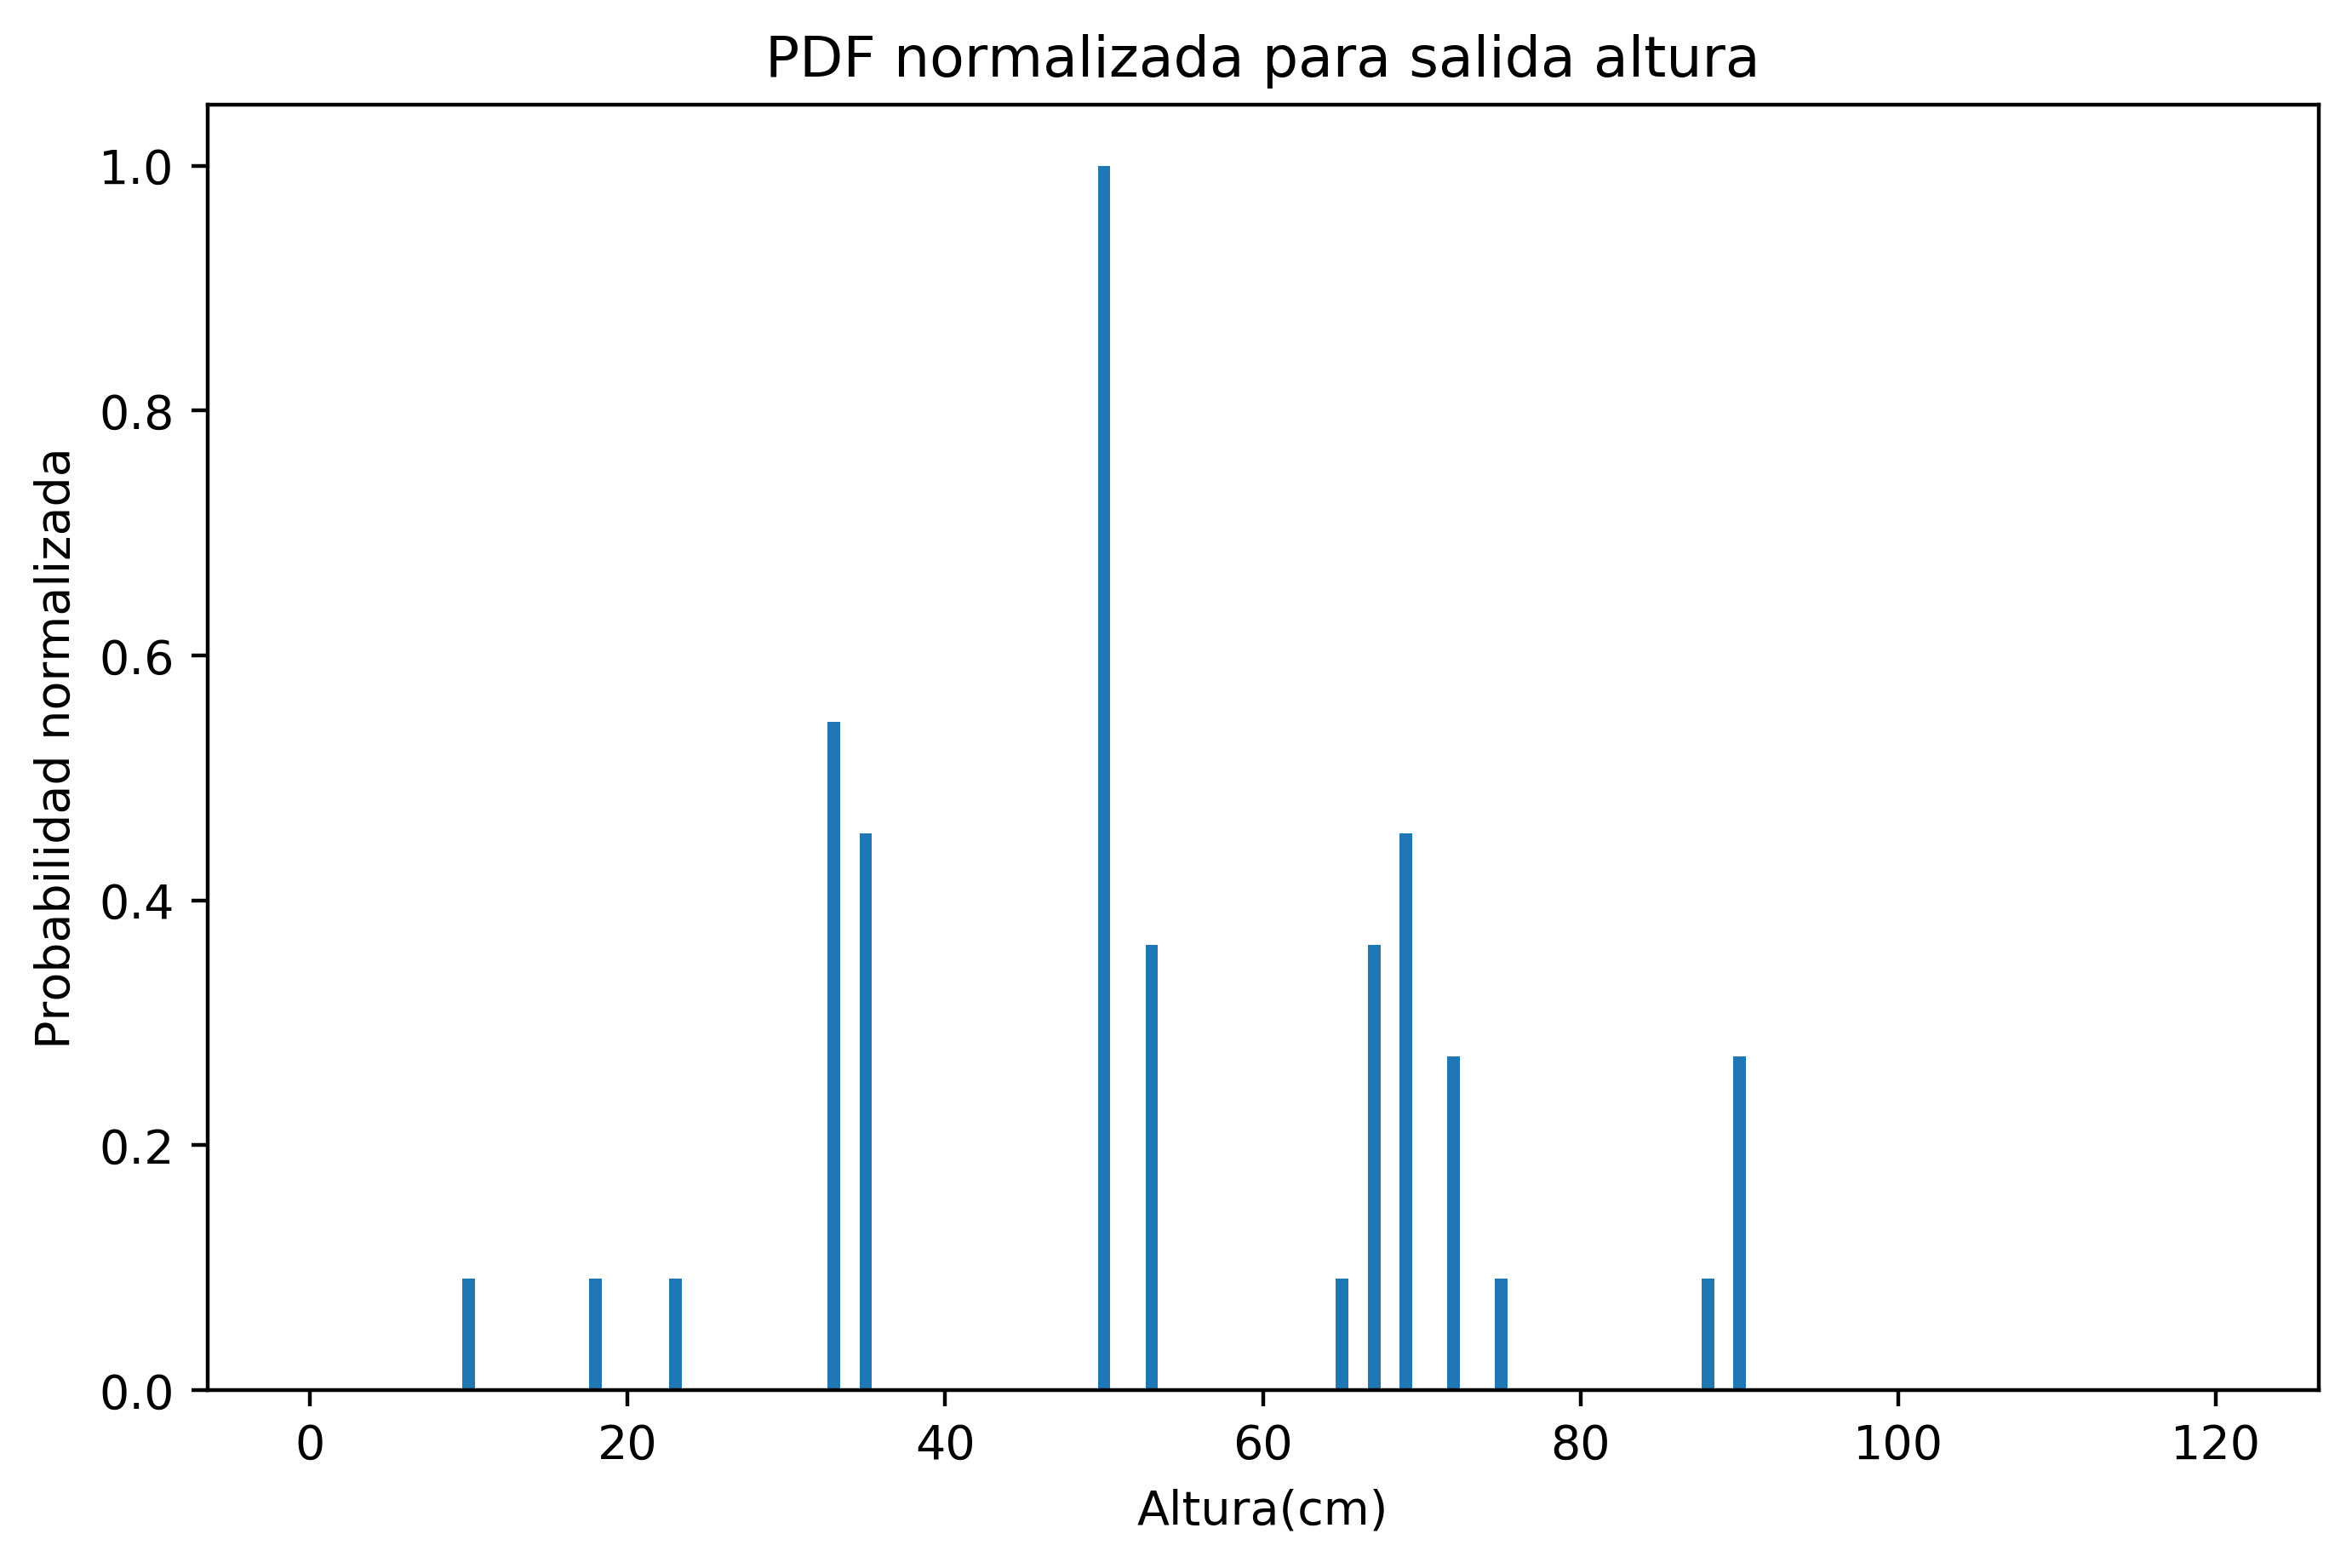
\includegraphics[width=0.95\linewidth]{archivos/tfg/Pixel/BBCHH_PDF_H}
  \caption{Ejemplo del modelo de doble salida: \gls{pdf} estimación de altura\label{fig:p_sub2}}
\end{subfigure}
\caption{Ejemplo de salidas \gls{pdf} normalizadas del modelo para estimación de \gls{bbch} y la altura. \label{fig:p_pdf_bh}}
\end{figure}

\subsubsection{Salidas de valor único}
\par Para continuar con la presentación de los resultados obtenidos, se ilustran en las figuras \ref{fig:p_comp_b}, \ref{fig:p_comp_h} y \ref{fig:p_comp_bh} las comparaciones de las soluciones únicas obtenidas (salida con máxima probabilidad) y los datos de tierra tomados correspondientes para la parcela de test en 2018: \gls{bbch} general, máxima y mínima en la parcela, casos individual (\ref{fig:comp_b}) y de doble salida (\ref{fig:p_sub_c1}), o la altura general del cultivo, también para ambos casos (figuras \ref{fig:p_comp_h} y \ref{fig:p_sub_c2}, respectivamente). Se ha realizado una adaptación en los datos para poder representarlos de esta manera, ya que aquí la estimación de valor único se realiza a nivel de pixel y no de parcela, como los datos para contrastar. Es por ello que, para una representación y comprensión más sencillas, se representa la media y la desviación estándar para los píxeles a nivel de parcela y día. 
\\
\par En este método ambos modelos son comparables para las dos salidas posibles ya que todos ellos comparten la misma parcela de test, por lo que se compara la eficiencia para los mismos datos. Comenzando por los modelos de predicción de \gls{bbch} representados en las figuras \ref{fig:p_comp_b} y \ref{fig:p_sub_c1}, se pueden observar estimaciones y errores de nuevo muy parecidos. Ambos modelos presentan una tendencia creciente, que estima a la baja la fenología para las últimas etapas del desarrollo y los mismos picos de predicción errónea sobre los días desde la siembra de 30-40 ya comentados anteriormente. Exceptuando las últimas etapas, se aprecian medias bastante cercanas a los valores reales, aunque con unas desviaciones estándar muy grandes a partir de los 40 días desde la siembra. Estas desviaciones se deben tanto a diferencias reales en la parcela, áreas con diferente nivel de desarrollo, como a un mal ajuste del modelo ya que en el entrenamiento existían estas diferencias en la misma parcela y se ha considerado el mismo valor de \gls{bbch} por la disponibilidad de datos de verdad de tierra. En esta metodología no aparecen diferencias tan claras entre los dos modelos implementados, ya que eran bastante similares. 
\\
\par Considerando las salidas para la altura, también se puede apreciar la gran similitud que presentan las representaciones comparadas: figuras \ref{fig:p_comp_h} y \ref{fig:p_sub_c2}, dificilmente diferenciables a simple vista. Las coincidencias más obvias son las mencionadas con la estimación de la \gls{bbch}: la tendencia creciente, los picos de predicciones erróneas para las mismas etapas y grandes desviaciones estándar, en este caso, durante todo el proceso. Hay que puntualizar, que las medias para cada parcela tienen valores muy próximos a los reales, sobretodo en las etapas intermedias y finales, cuando la mayoría de los modelos presentan mayor inexactitud. Aunque los resultados globales evaluados para la metodología a nivel de pixel puedan ser numéricamente peores debido a la evaluación independiente de cada pixel, este es el método que mejores resultados ha obtenido para la estimación de la altura.

% Una figura con dos imágenes
\begin{figure}[H]
\centering
\begin{subfigure}{.85\textwidth}
  \centering
  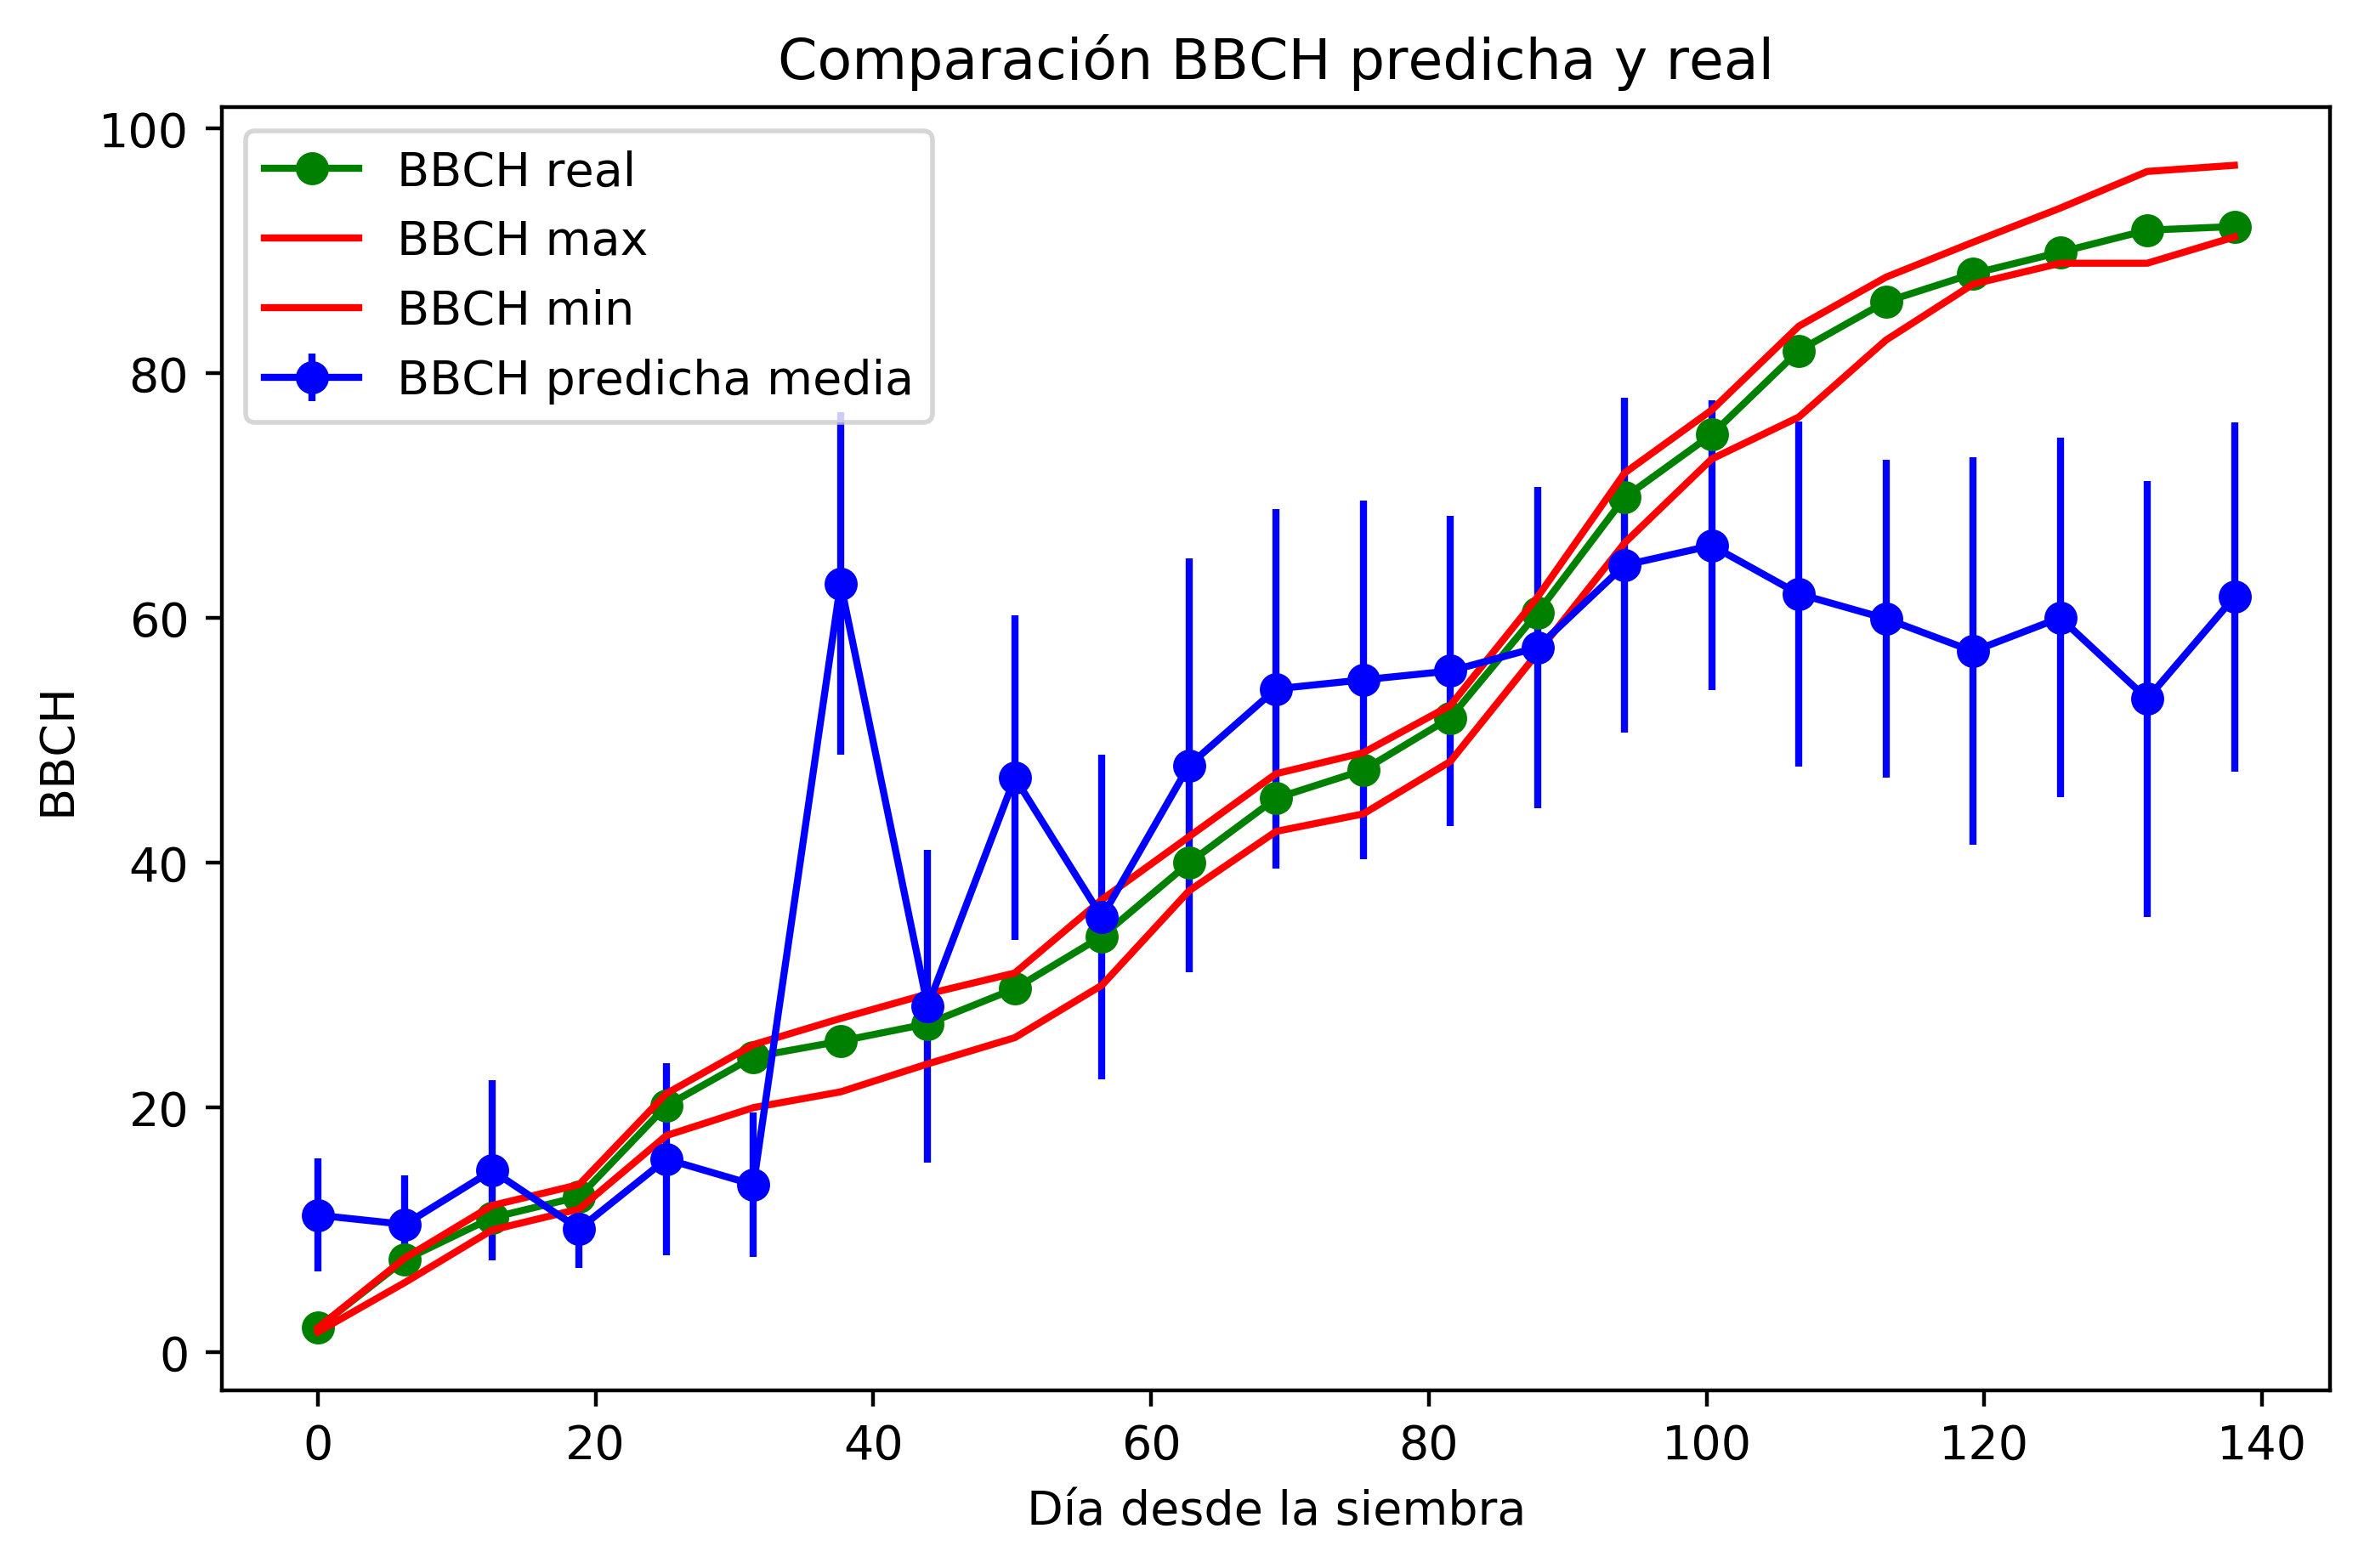
\includegraphics[width=0.95\linewidth]{archivos/tfg/Pixel/BBCH_COMPARACION_BIEN}
  \caption{Comparación de la salida predicha y la verdad de tierra del modelo para estimación de la \gls{bbch}. \label{fig:p_comp_b}}
\end{subfigure}
\begin{subfigure}{.85\textwidth}
  \centering
  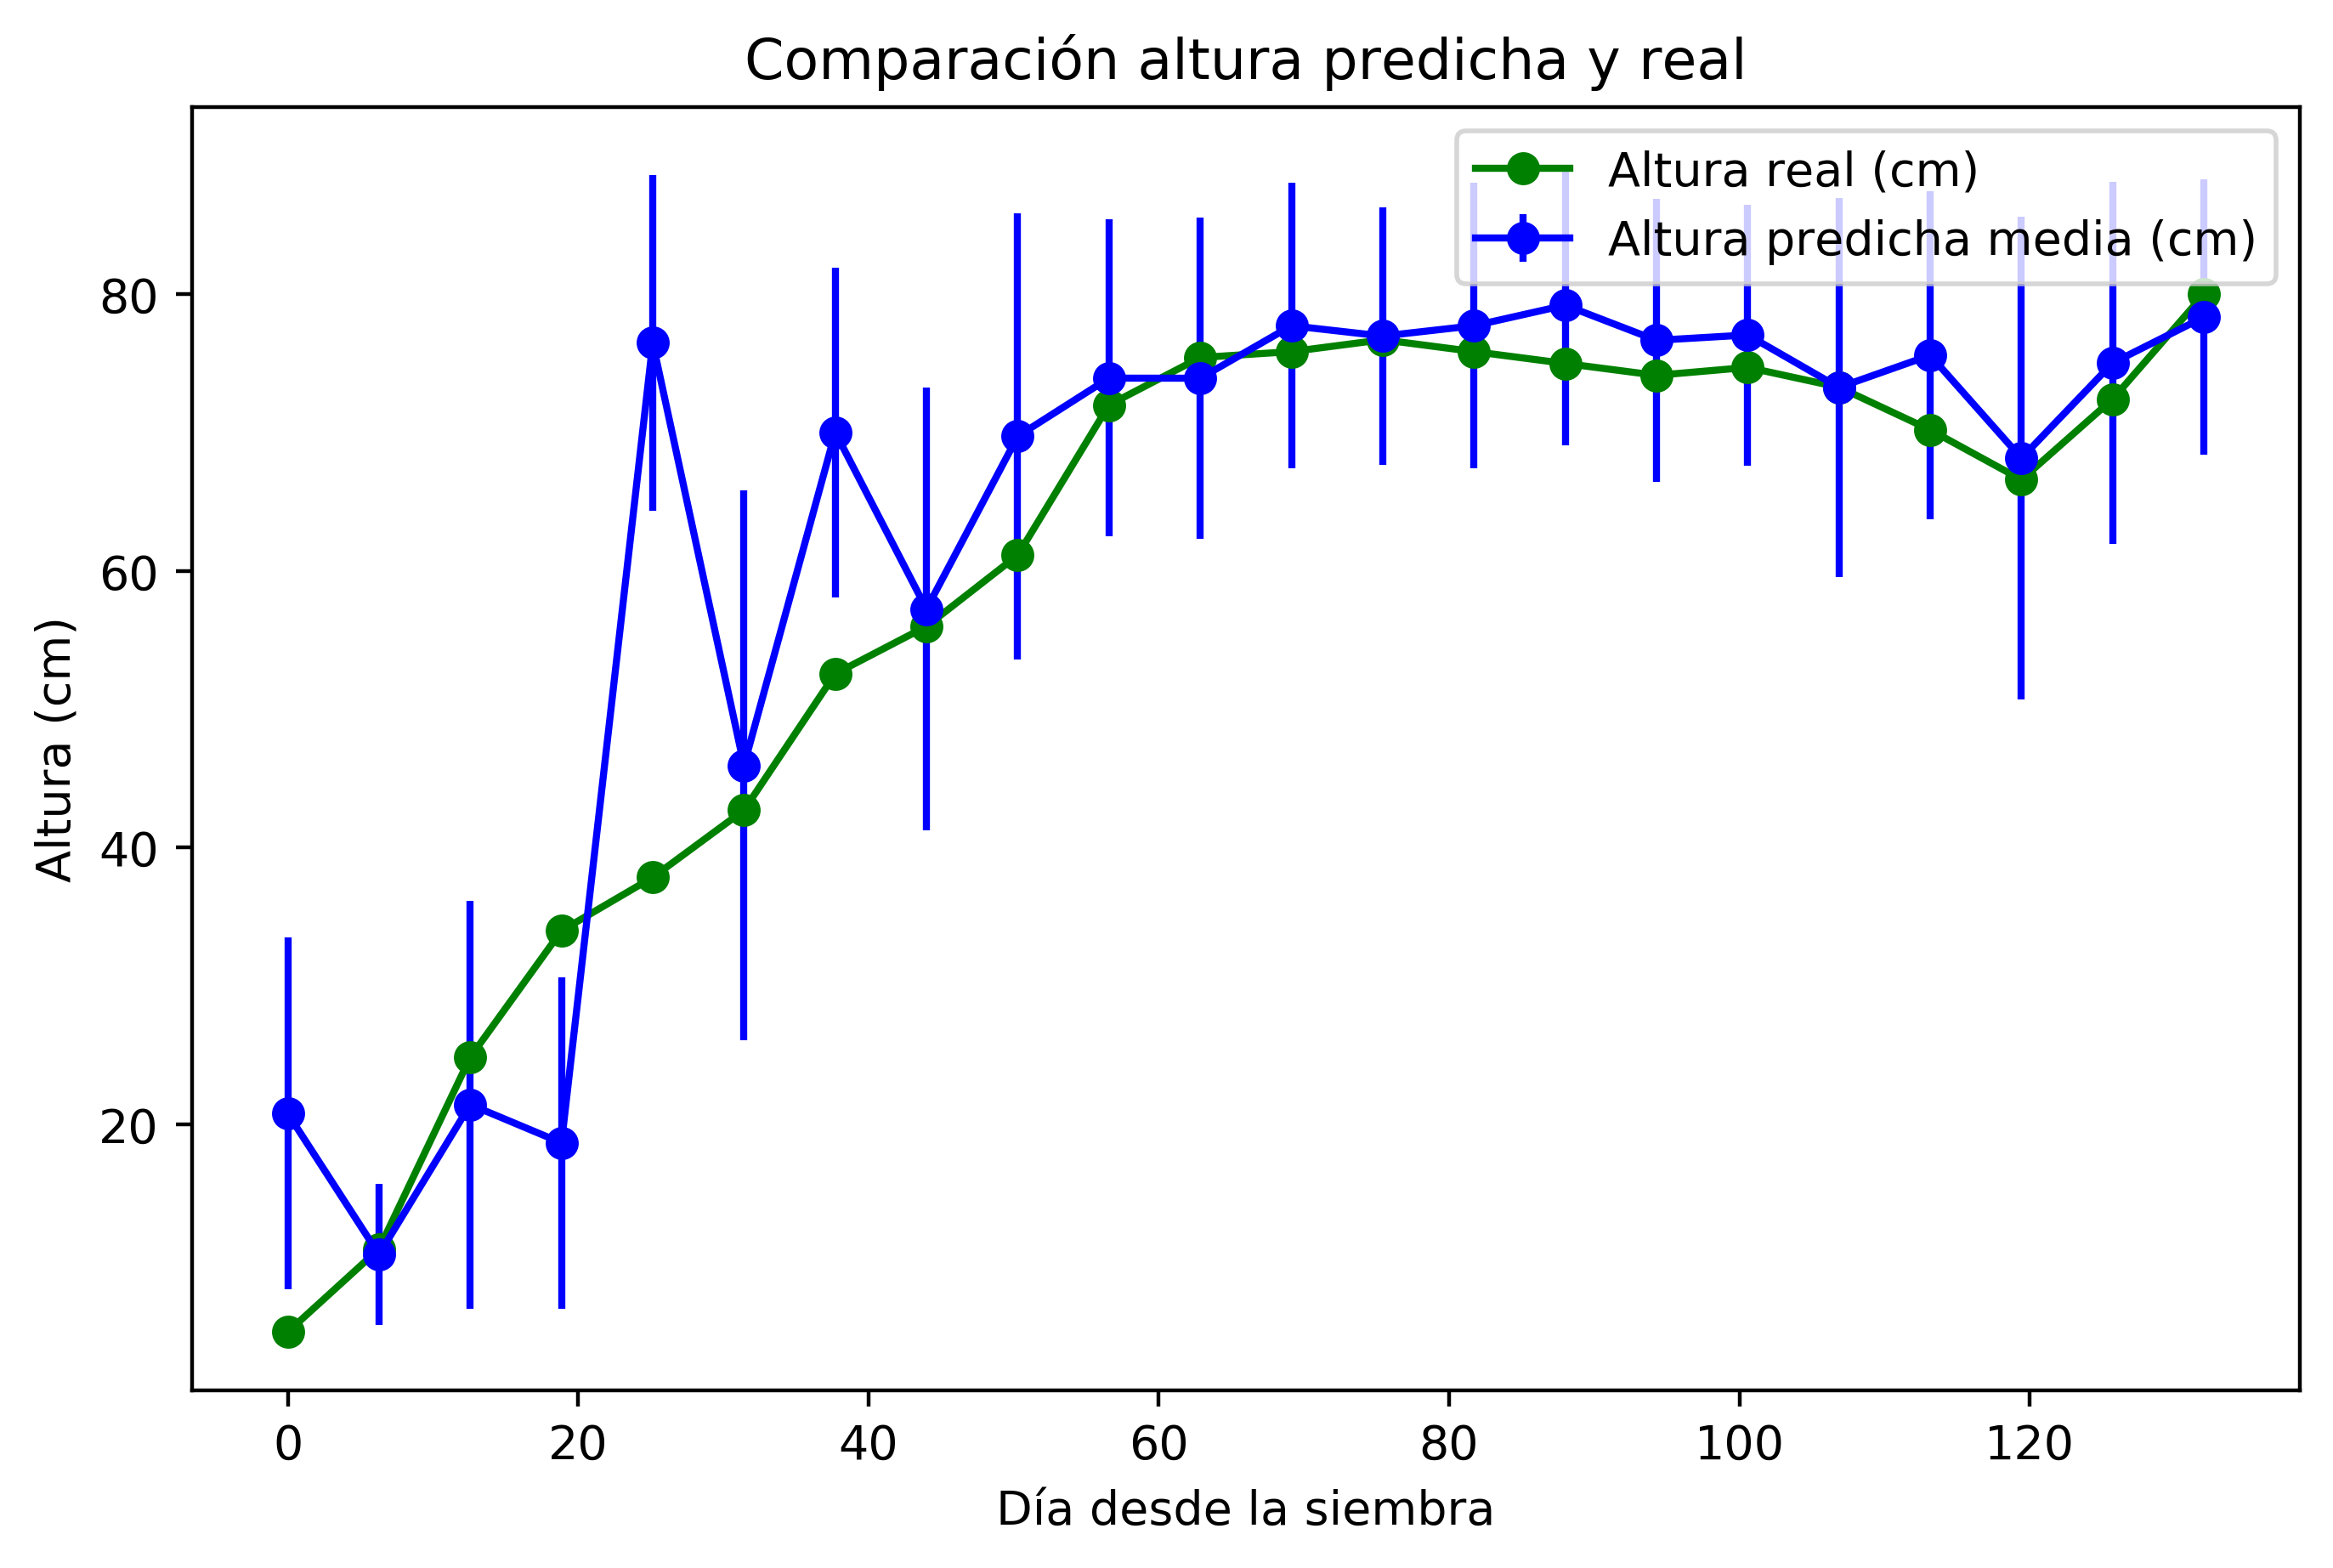
\includegraphics[width=0.95\linewidth]{archivos/tfg/Pixel/H_COMPARACION_BIEN}
  \caption{Comparación de la salida predicha y la verdad de tierra del modelo de doble salida para la estimación de la altura\label{fig:p_comp_h}}
\end{subfigure}
\caption{Comparación de la salida predicha y la verdad de tierra de los modelos de salidas individuales. \label{fig:p_comp}}
\end{figure}

% Una figura con dos imágenes
\begin{figure}[H]
\centering
\begin{subfigure}{.85\textwidth}
  \centering
  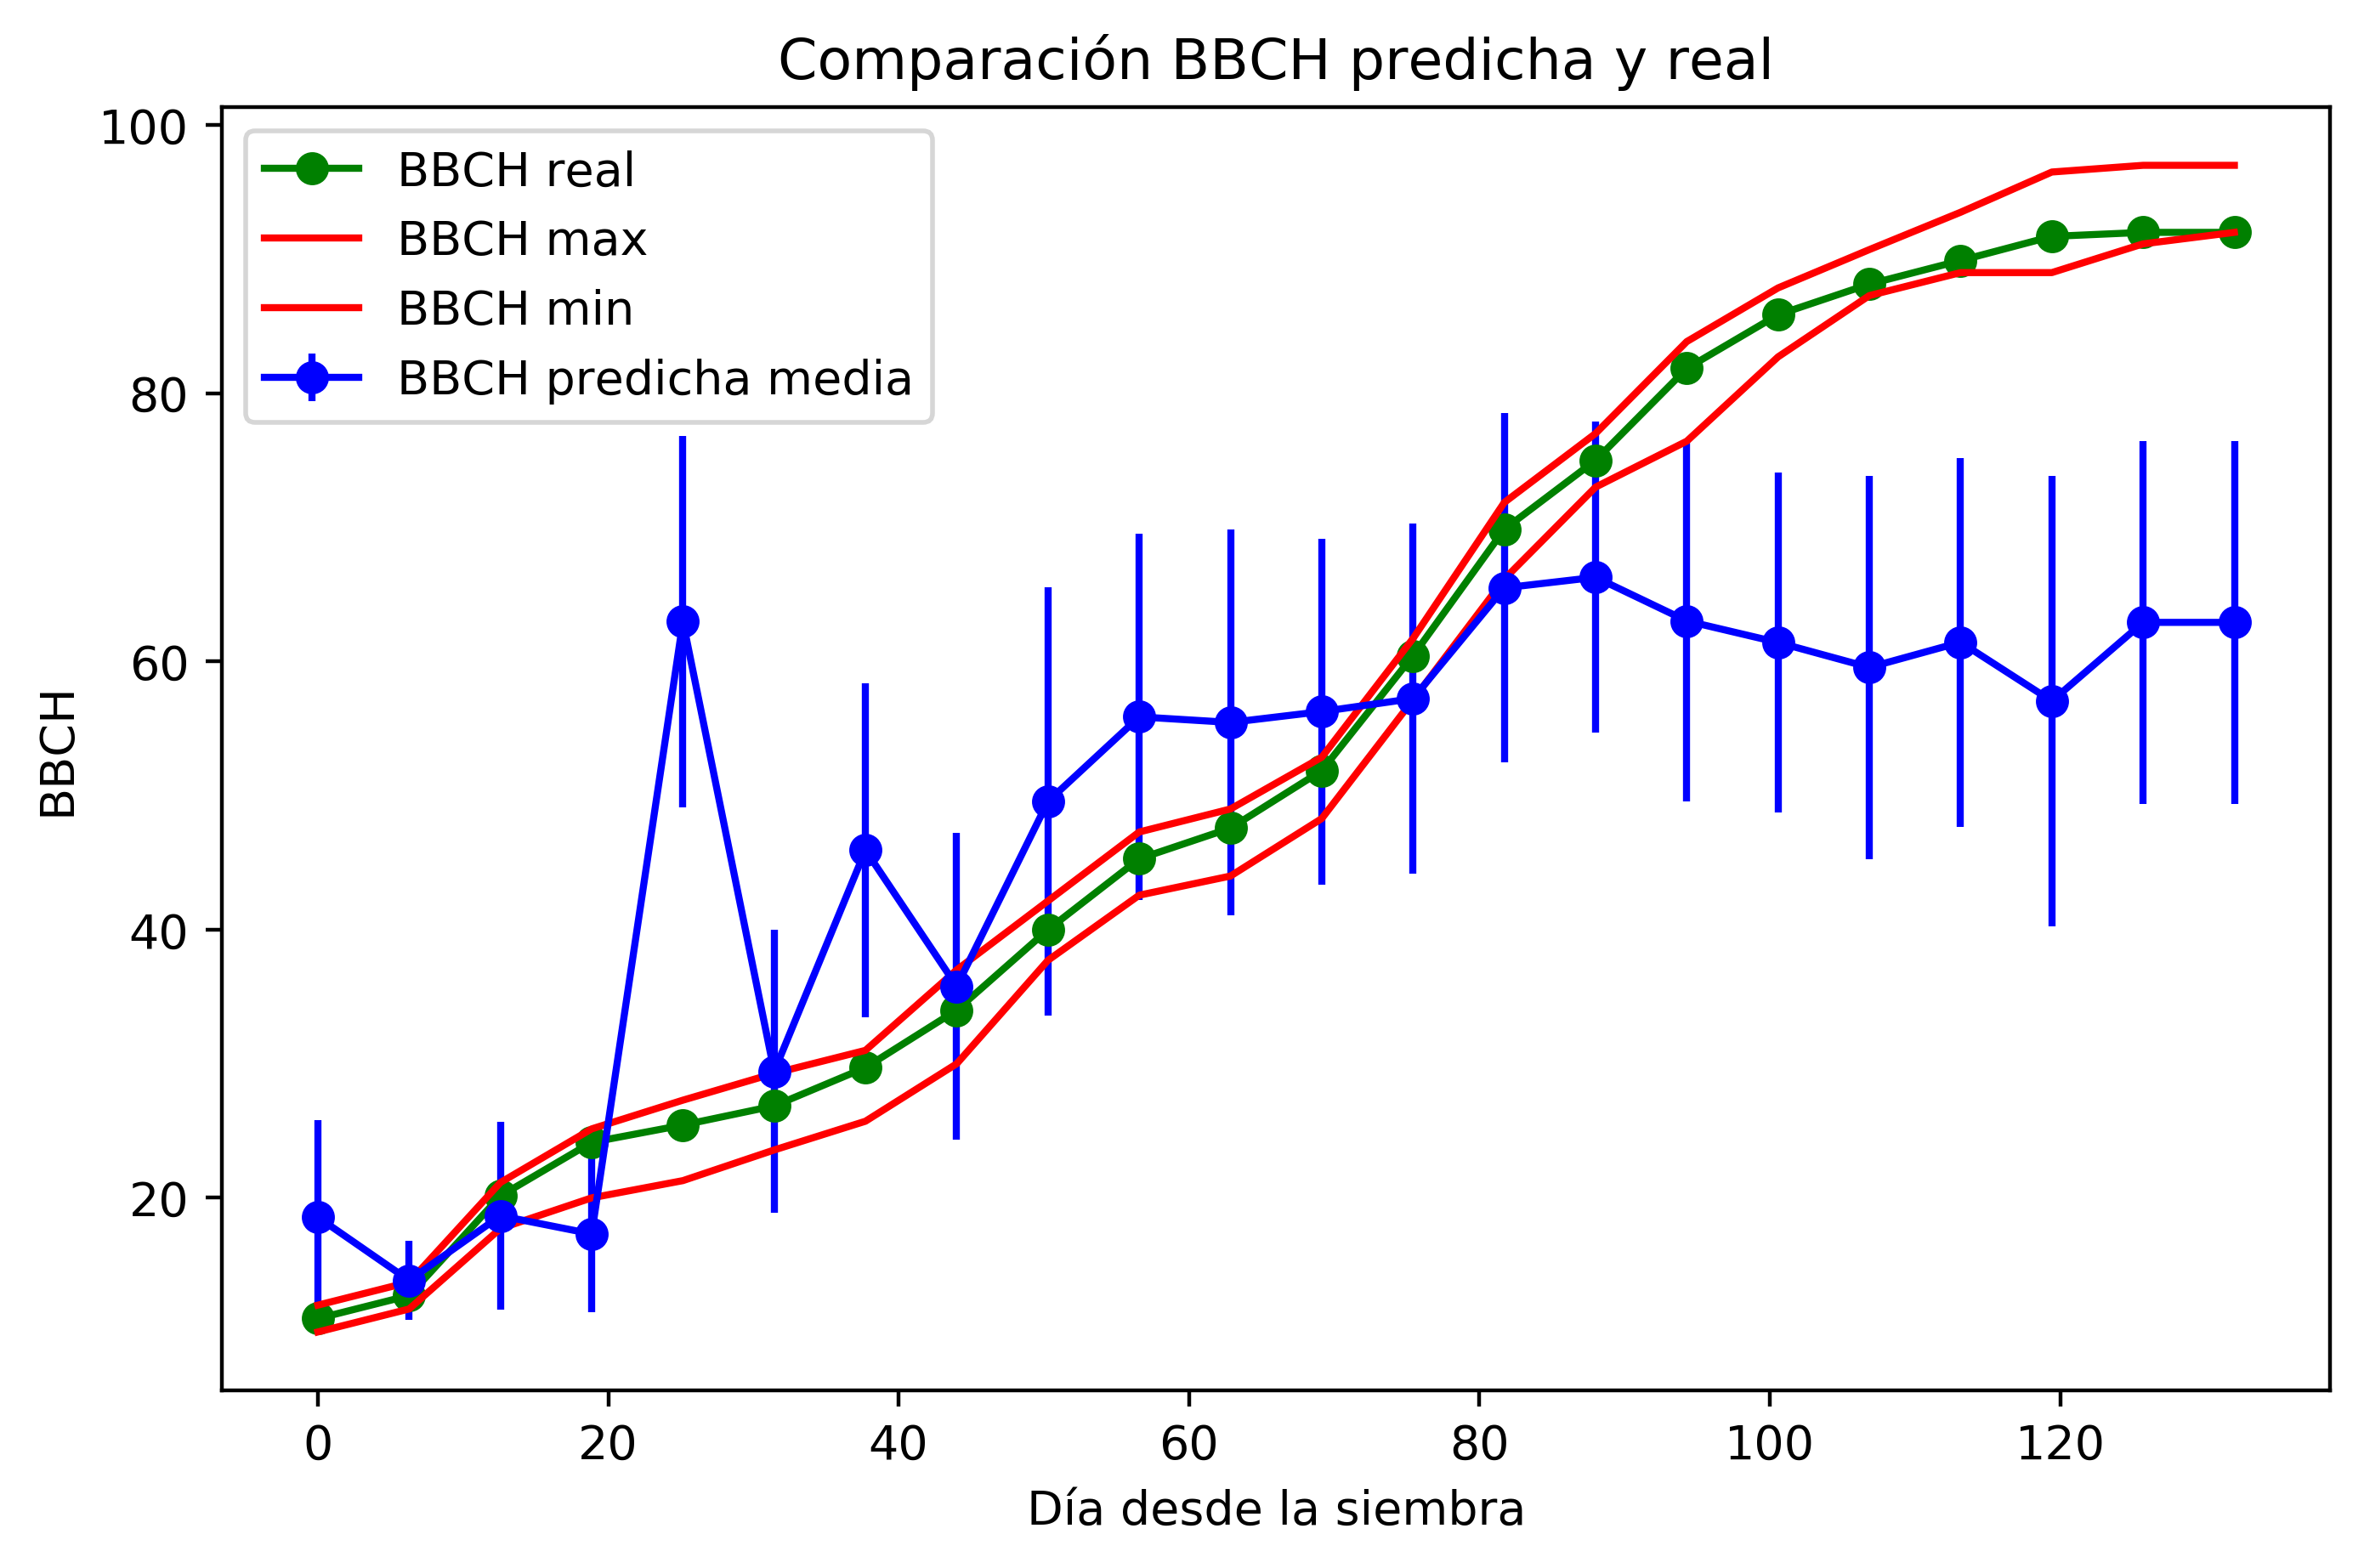
\includegraphics[width=0.95\linewidth]{archivos/tfg/Pixel/BBCHH_COMPARACION_BIEN_BBCH}
  \caption{Comparación de la salida predicha y la verdad de tierra del modelo de doble salida para la estimación de \gls{bbch}. \label{fig:p_sub_c1}}
\end{subfigure}

\begin{subfigure}{.85\textwidth}
  \centering
  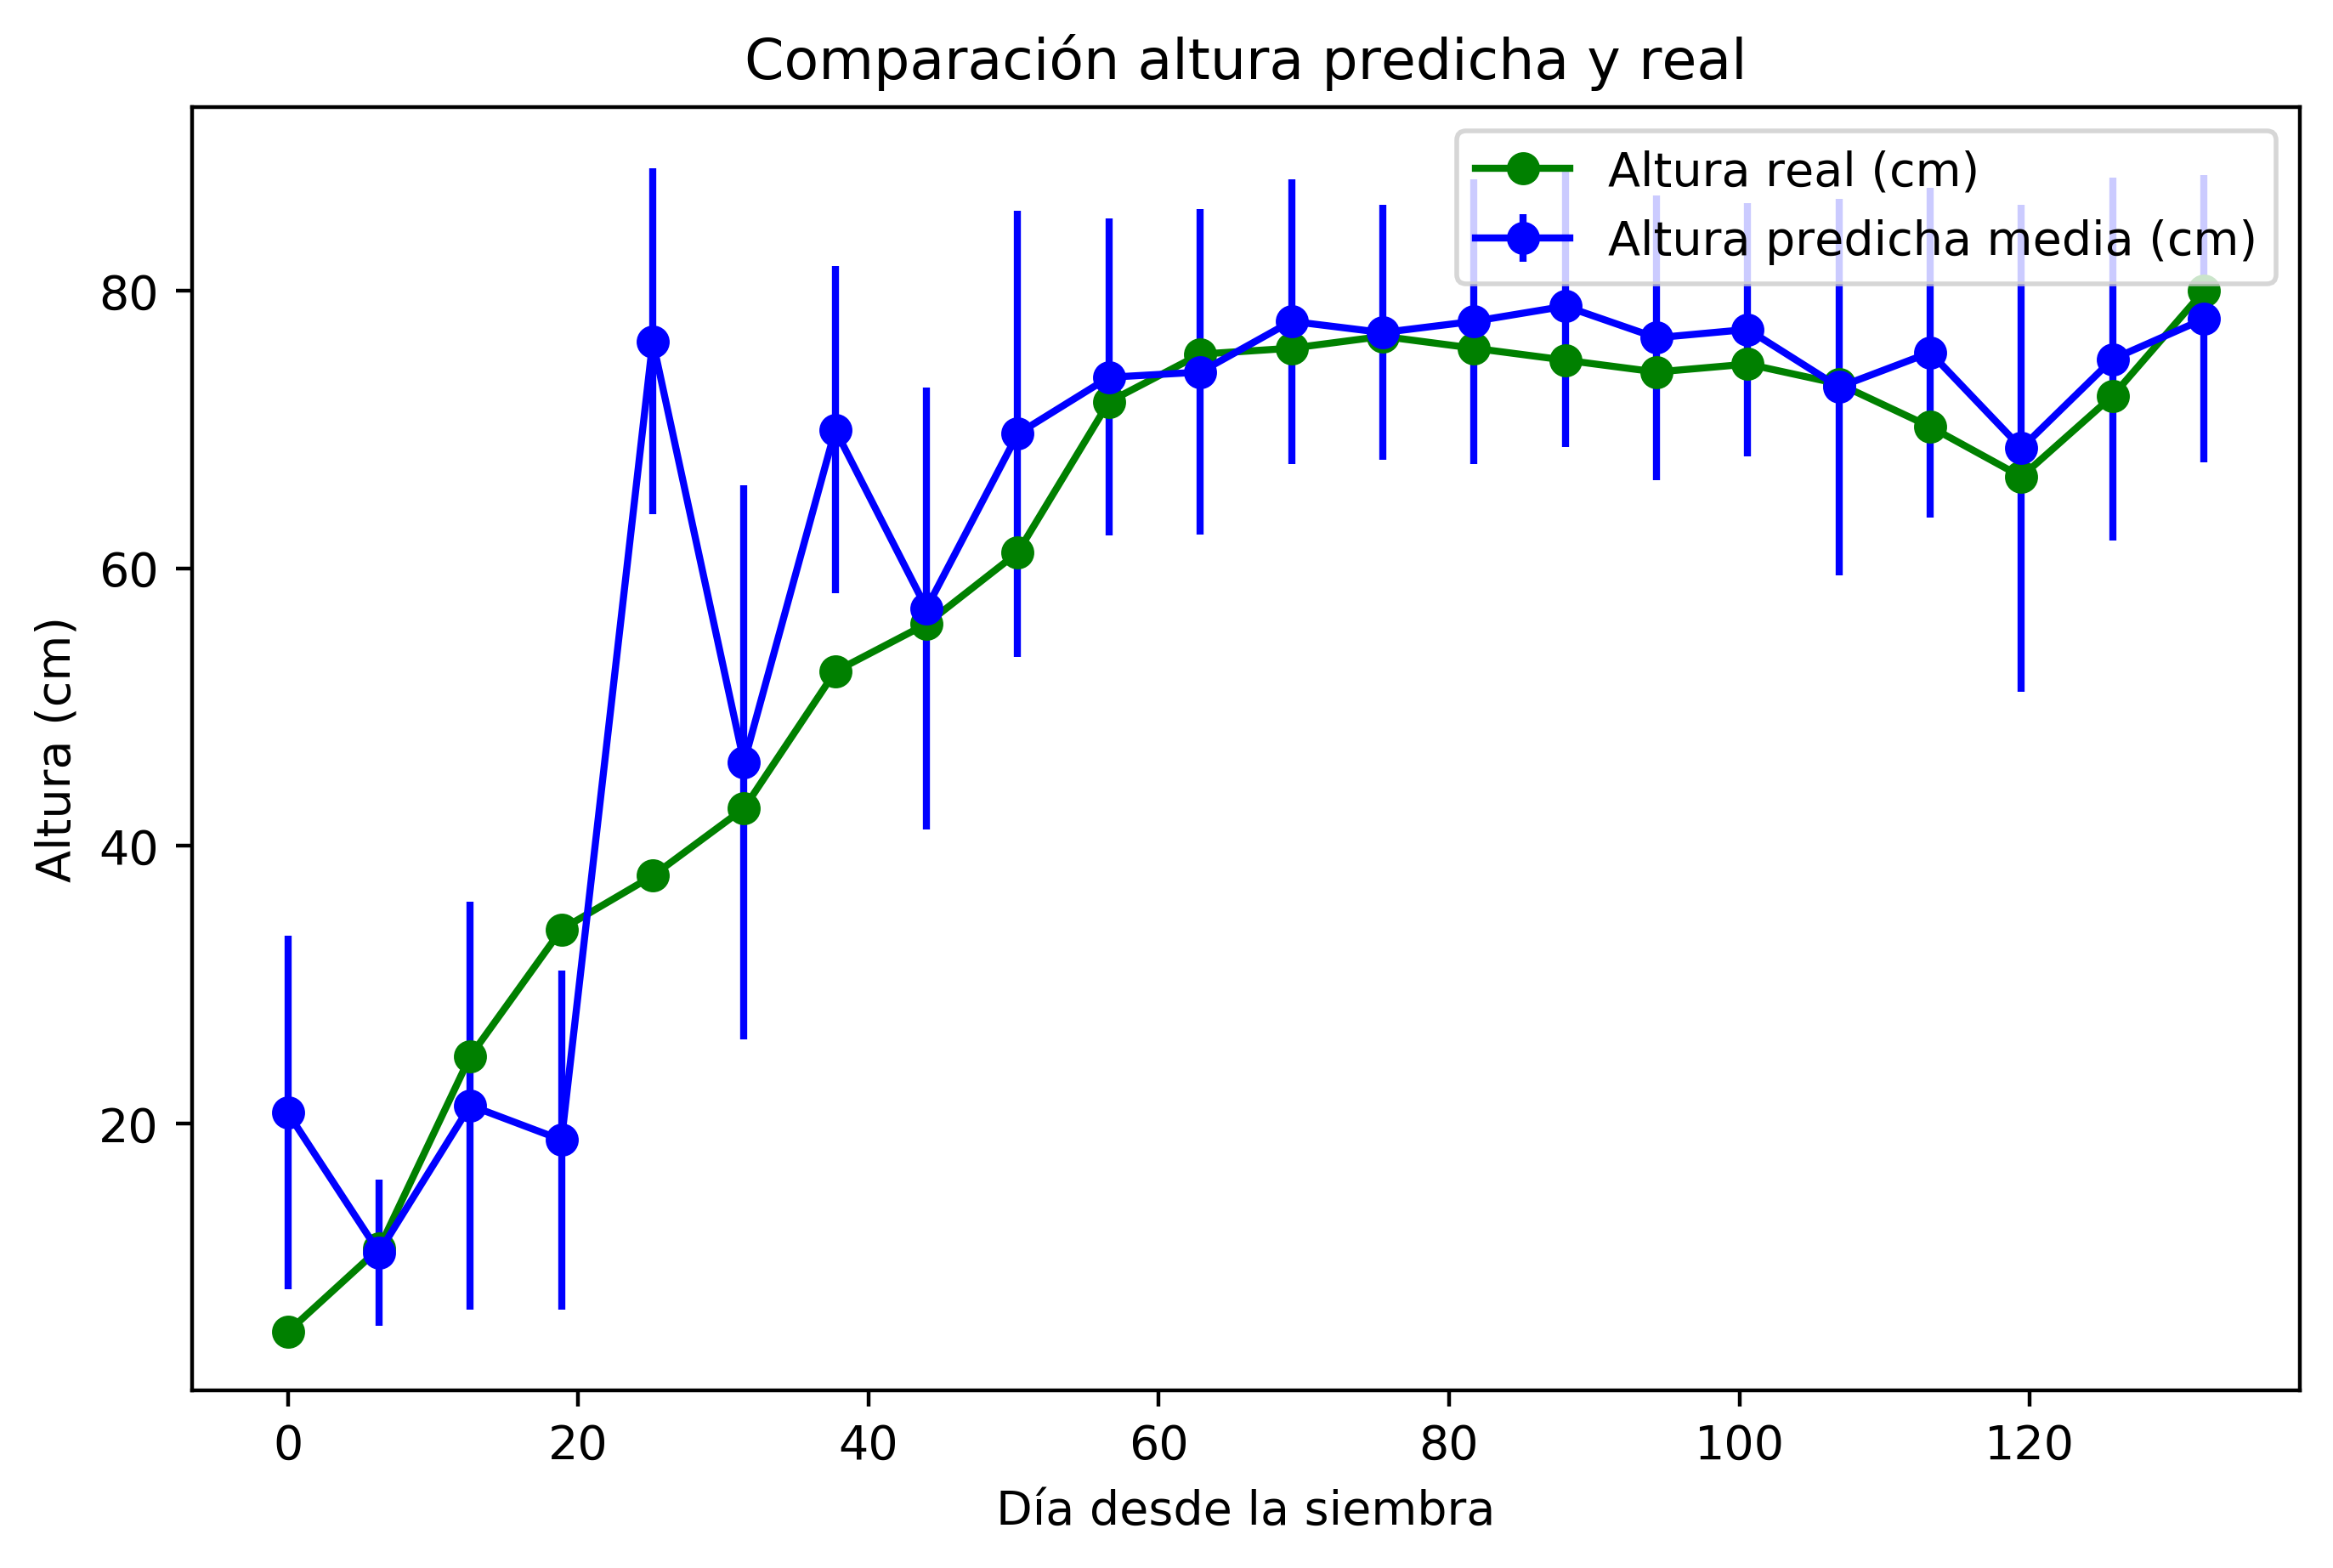
\includegraphics[width=0.95\linewidth]{archivos/tfg/Pixel/BBCHH_COMPARACION_BIEN_H}
  \caption{Comparación de la salida predicha y la verdad de tierra del modelo de doble salida para la estimación de la altura\label{fig:p_sub_c2}}
\end{subfigure}
\caption{Comparación de la salida predicha y la verdad de tierra del modelo de doble salida para la estimación de \gls{bbch} y la altura. \label{fig:p_comp_bh}}
\end{figure}

\subsection{Evaluación de resultados}
\par Para la evaluación de los resultados obtenidos para el método por píxeles se van a utilizar, como se ha mencionado anteriormente, las salidas de valor único por su facilidad para ser representadas y comparadas con los valores únicos medidos. 
\\
\begin{figure}[H]
\centering
\begin{subfigure}{.7\textwidth}
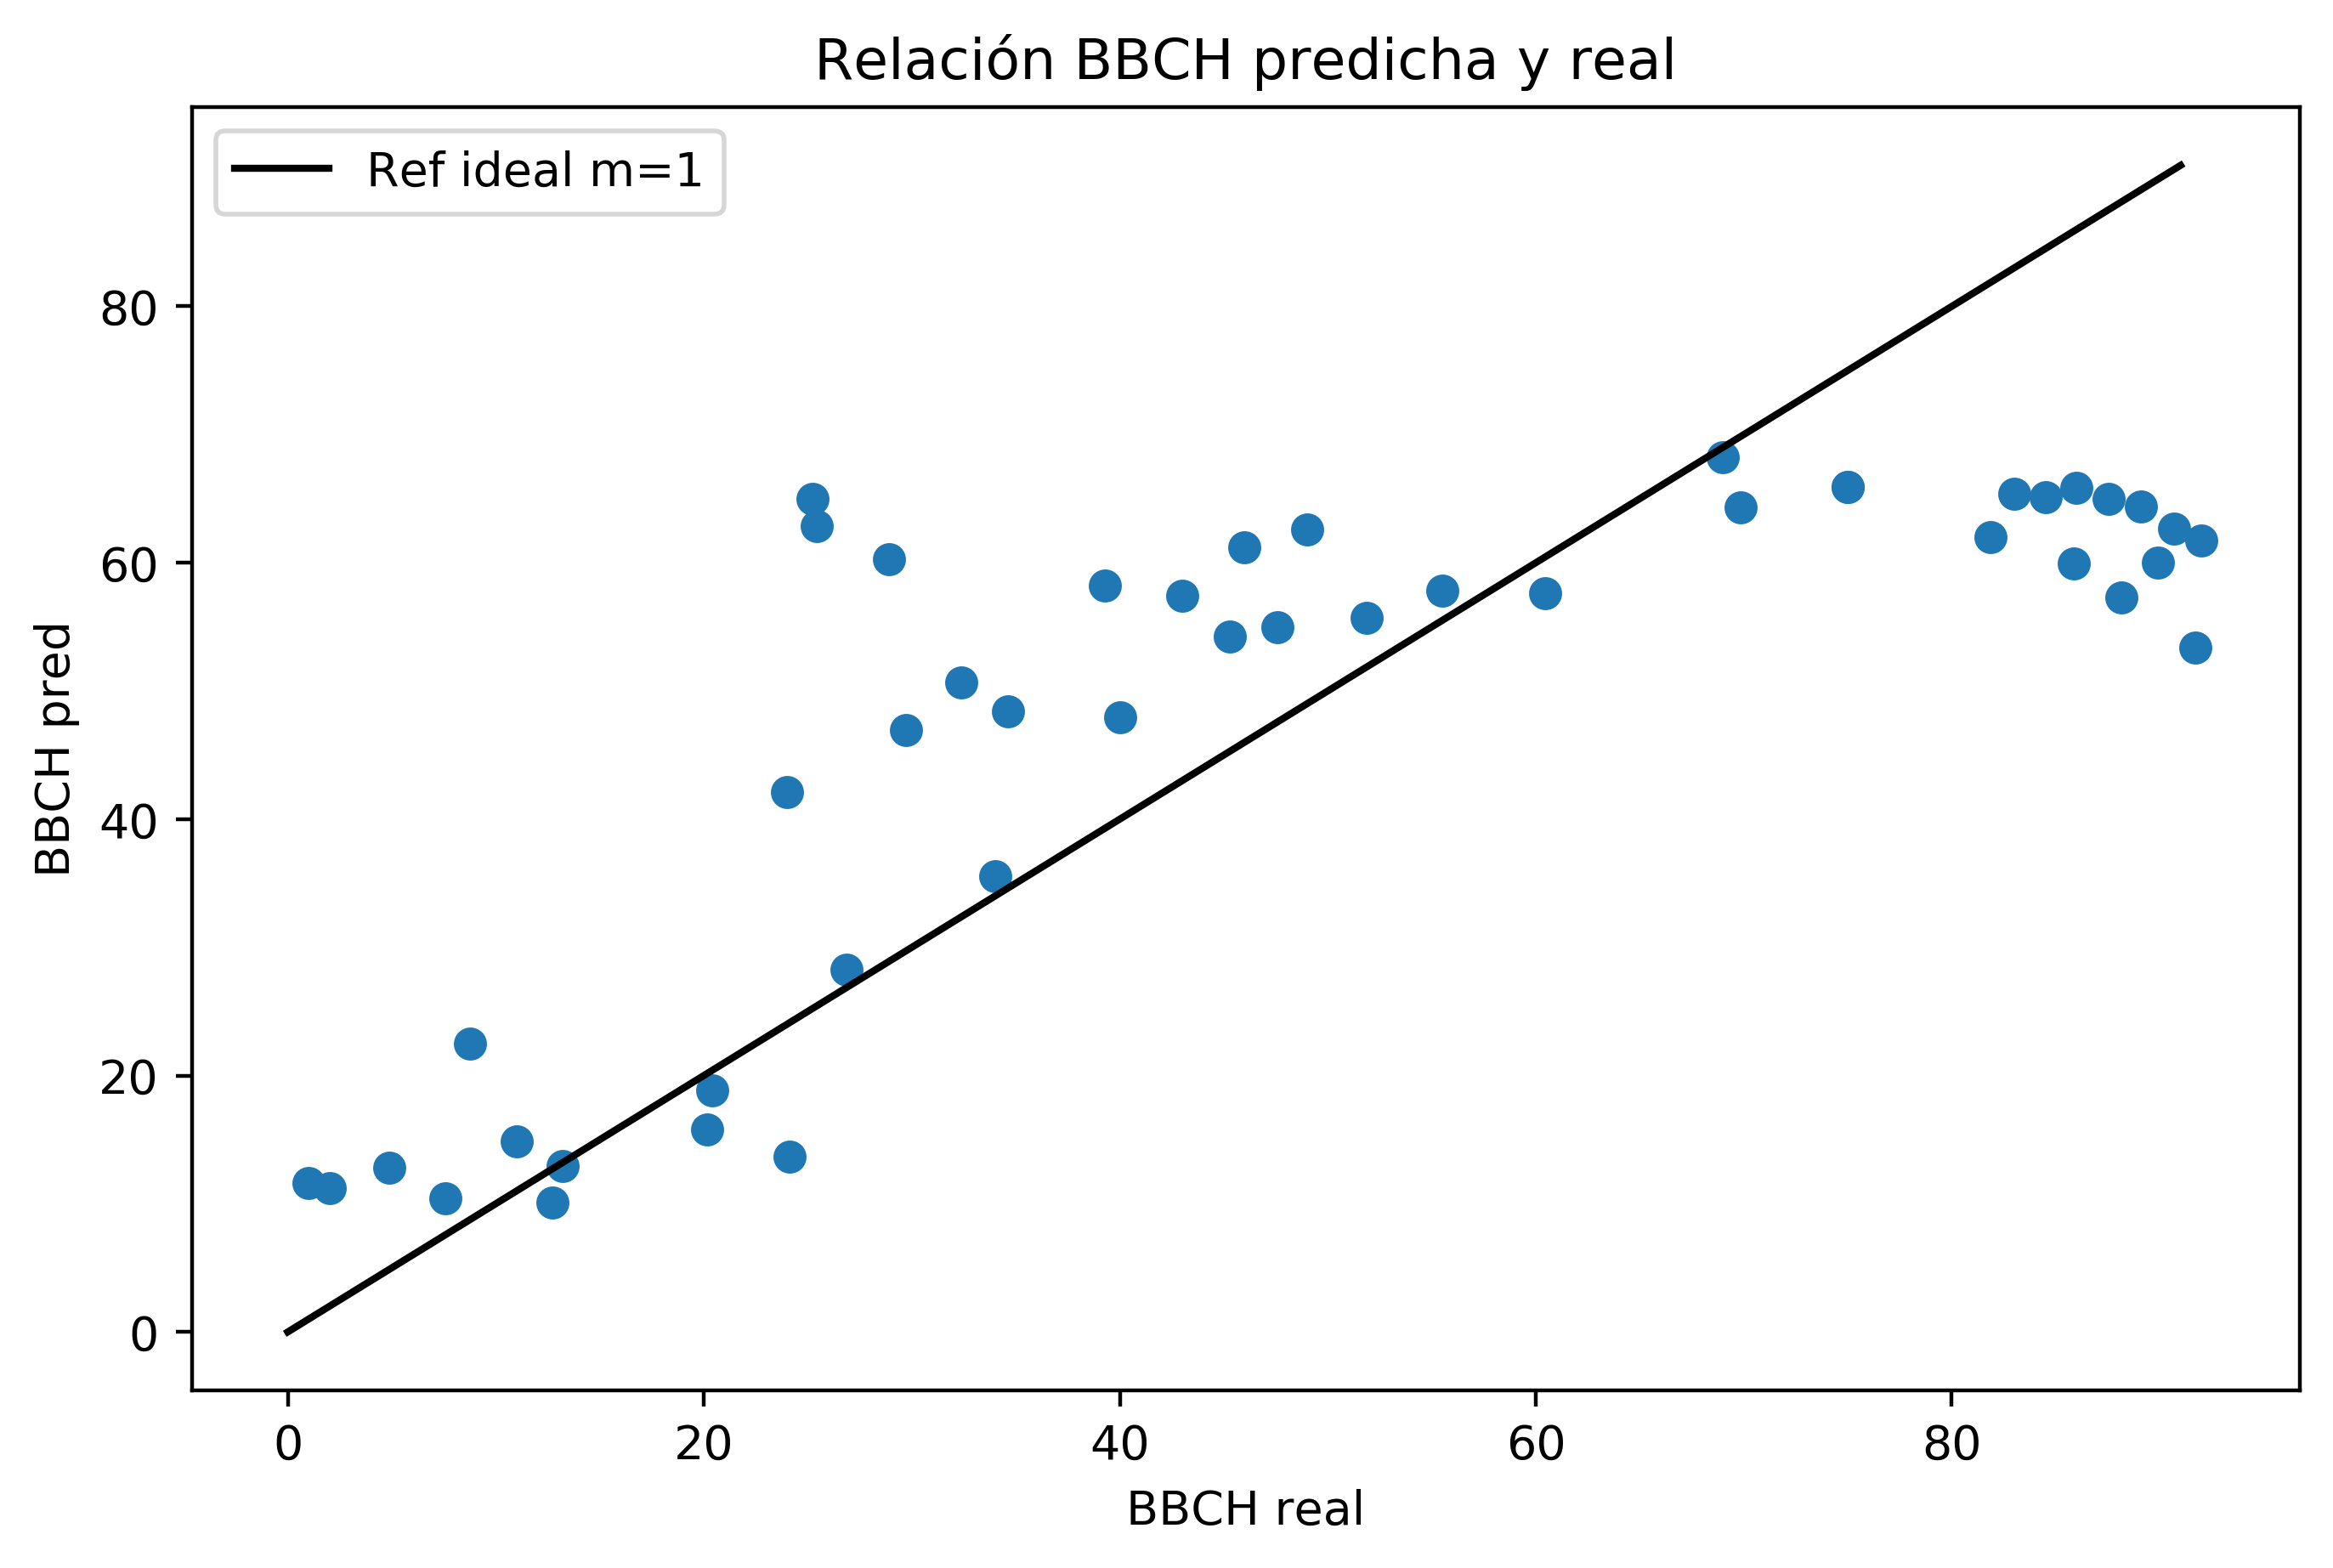
\includegraphics[width=0.95\linewidth]{archivos/tfg/Pixel/BBCH_RELACION_BIEN}
\captionof{figure}{Relación de la salida predicha y la verdad de tierra del modelo para estimación de \gls{bbch}.\label{fig:p_rel_b}}
\end{subfigure}
\begin{subfigure}{.7\textwidth}
\centering
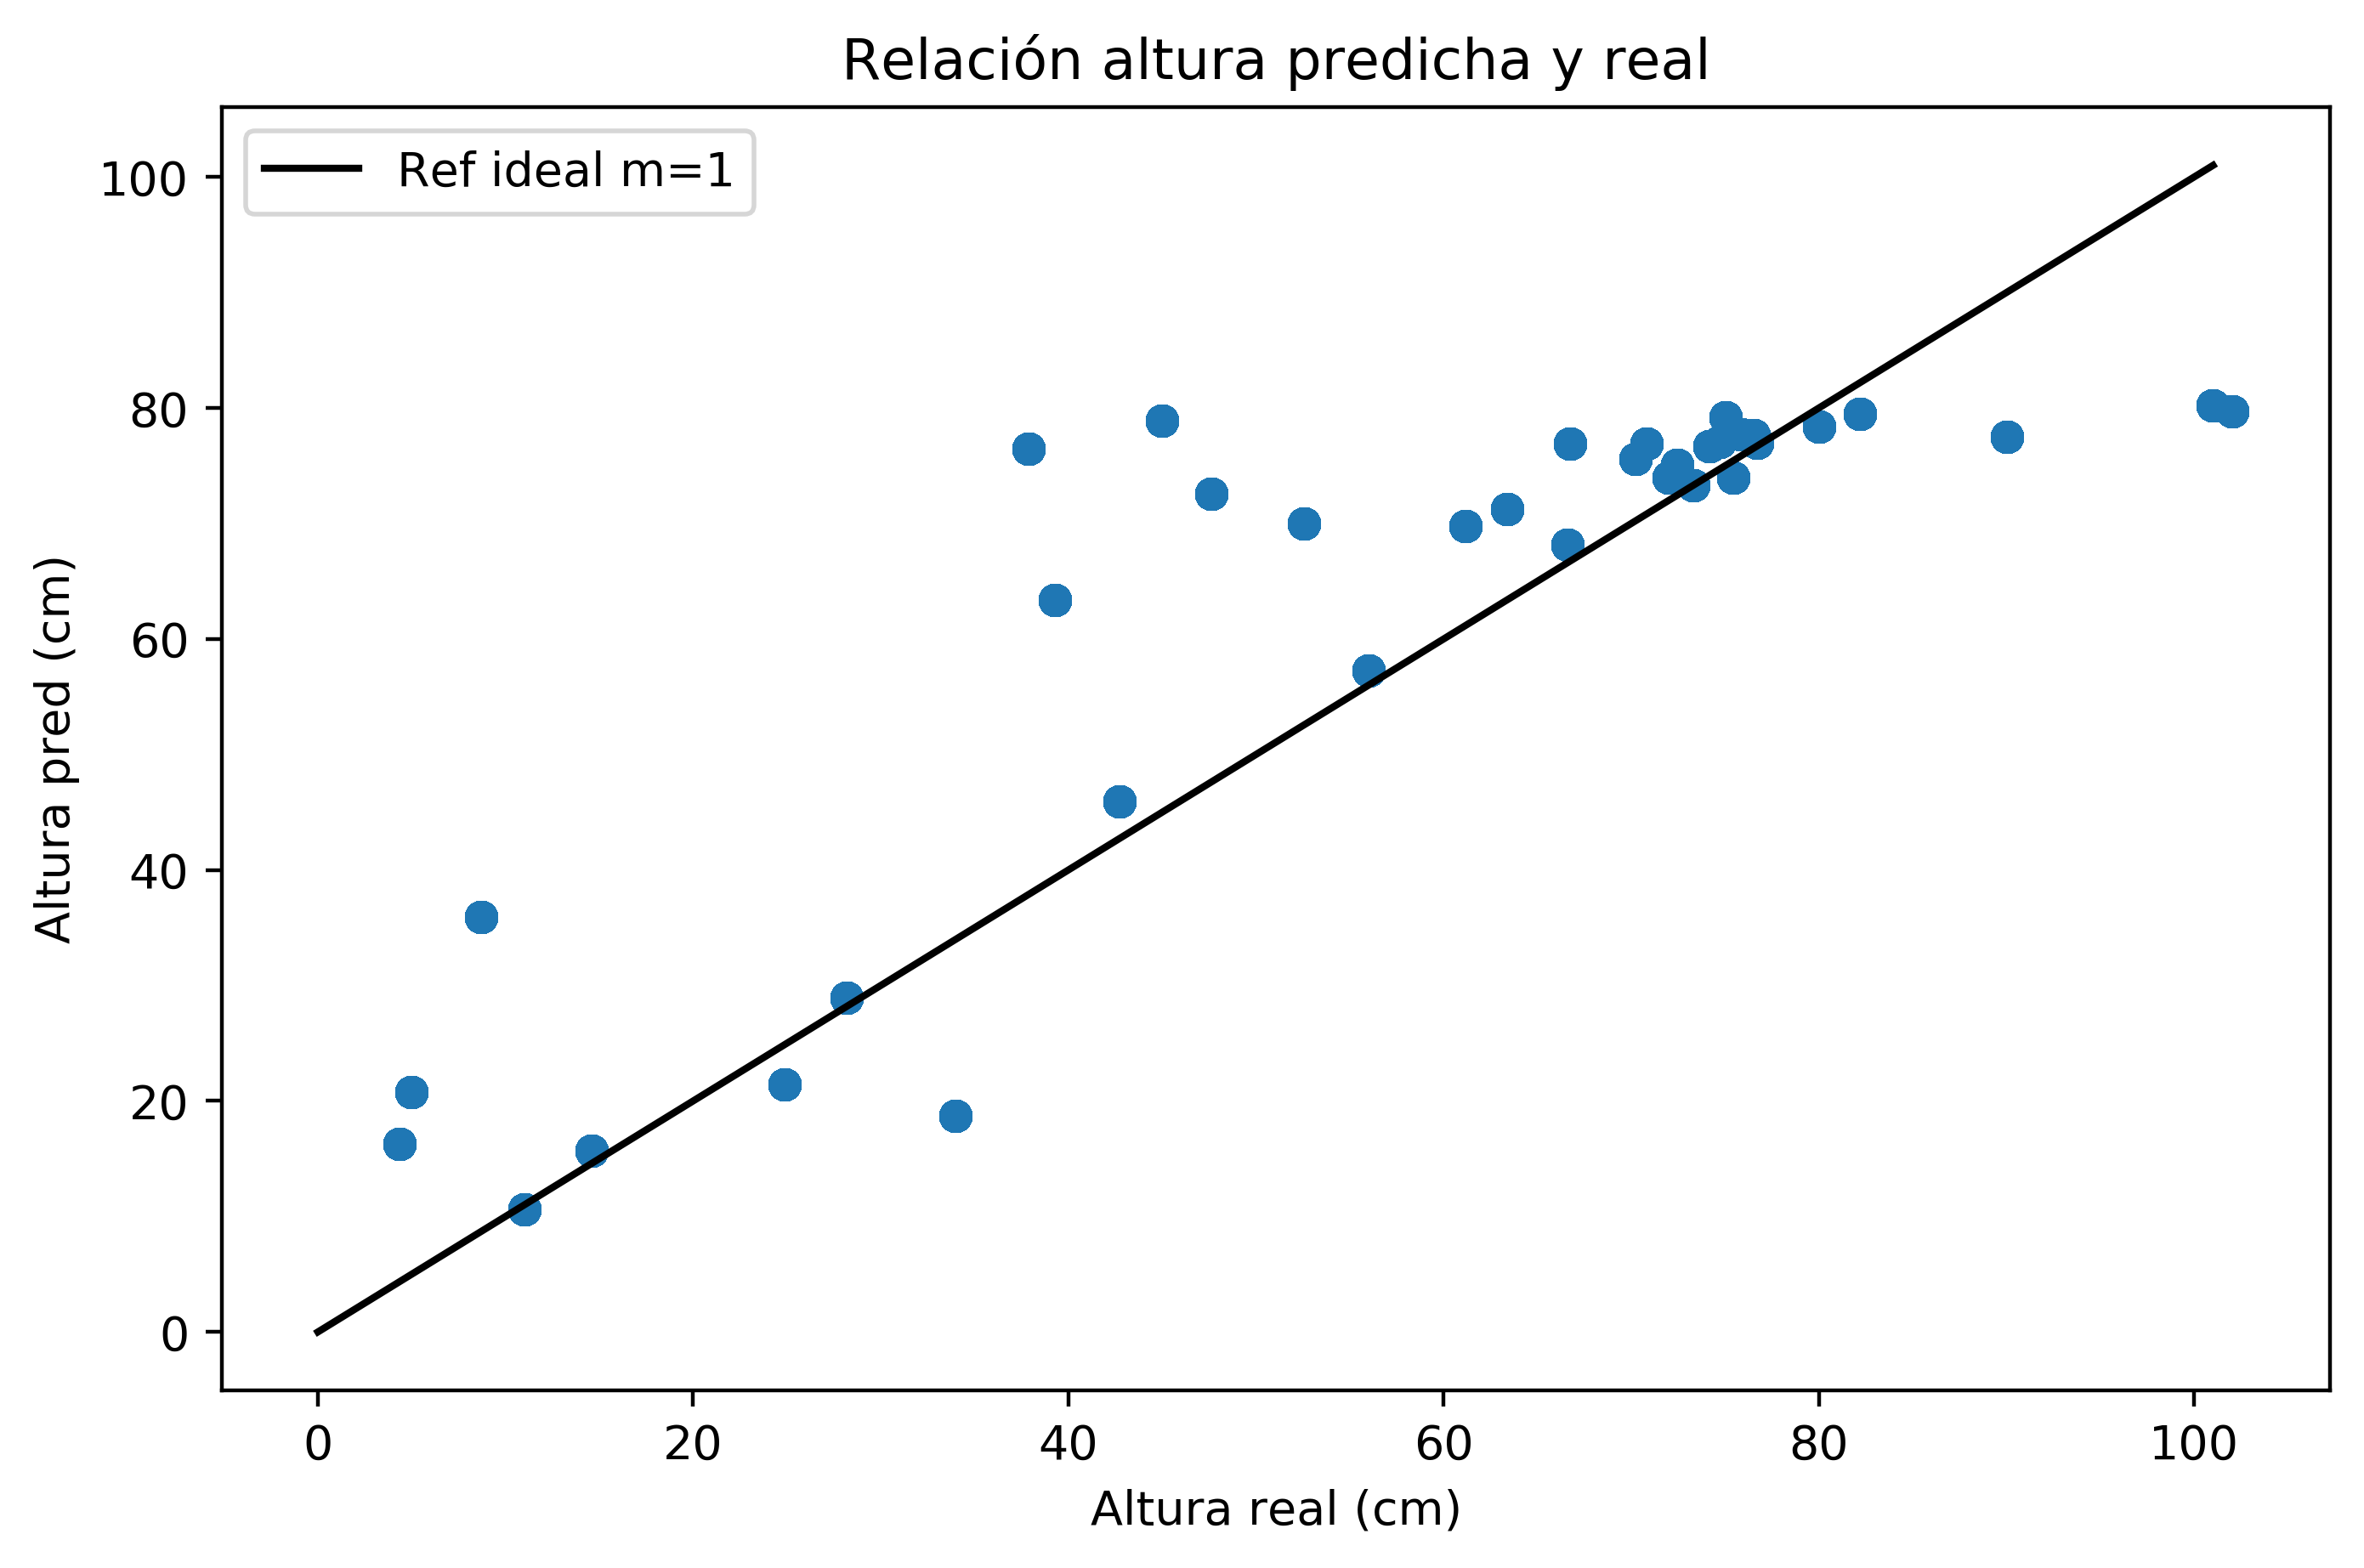
\includegraphics[width=0.95\linewidth]{archivos/tfg/Pixel/H_RELACION_BIEN}
\captionof{figure}{Relación de la salida predicha y la verdad de tierra del modelo para estimación de la altura. \label{fig:p_rel_h}}
\end{subfigure}
\captionof{figure}{Relación de la salida predicha y la verdad de tierra de los modelos de salidas independientes. \label{fig:p_rel_2}}
\end{figure}
\par Se realiza la primera evaluación, la relación directa entre las salidas estimadas medias por día y las medidas reales, en las figuras \ref{fig:p_rel_b}, para el modelo de única salida de \gls{bbch}, \ref{fig:p_rel_h}, para el modelo de única salida de altura y la figura \ref{fig:p_rel_bh} para el modelo de doble salida. Se incluye en ellas, igualmete, la recta de referencia de pendiente ($m$) unidad, como modelo ideal. Se han utilizado para todas las representaciones los valores contrastados de la parcela de test correspondiente a cada caso, teniendo en cuenta ambos años de datos, 2017 y 2018.
\\
\begin{figure}[H]
\centering
\begin{subfigure}{0.7\textwidth}
  \centering
  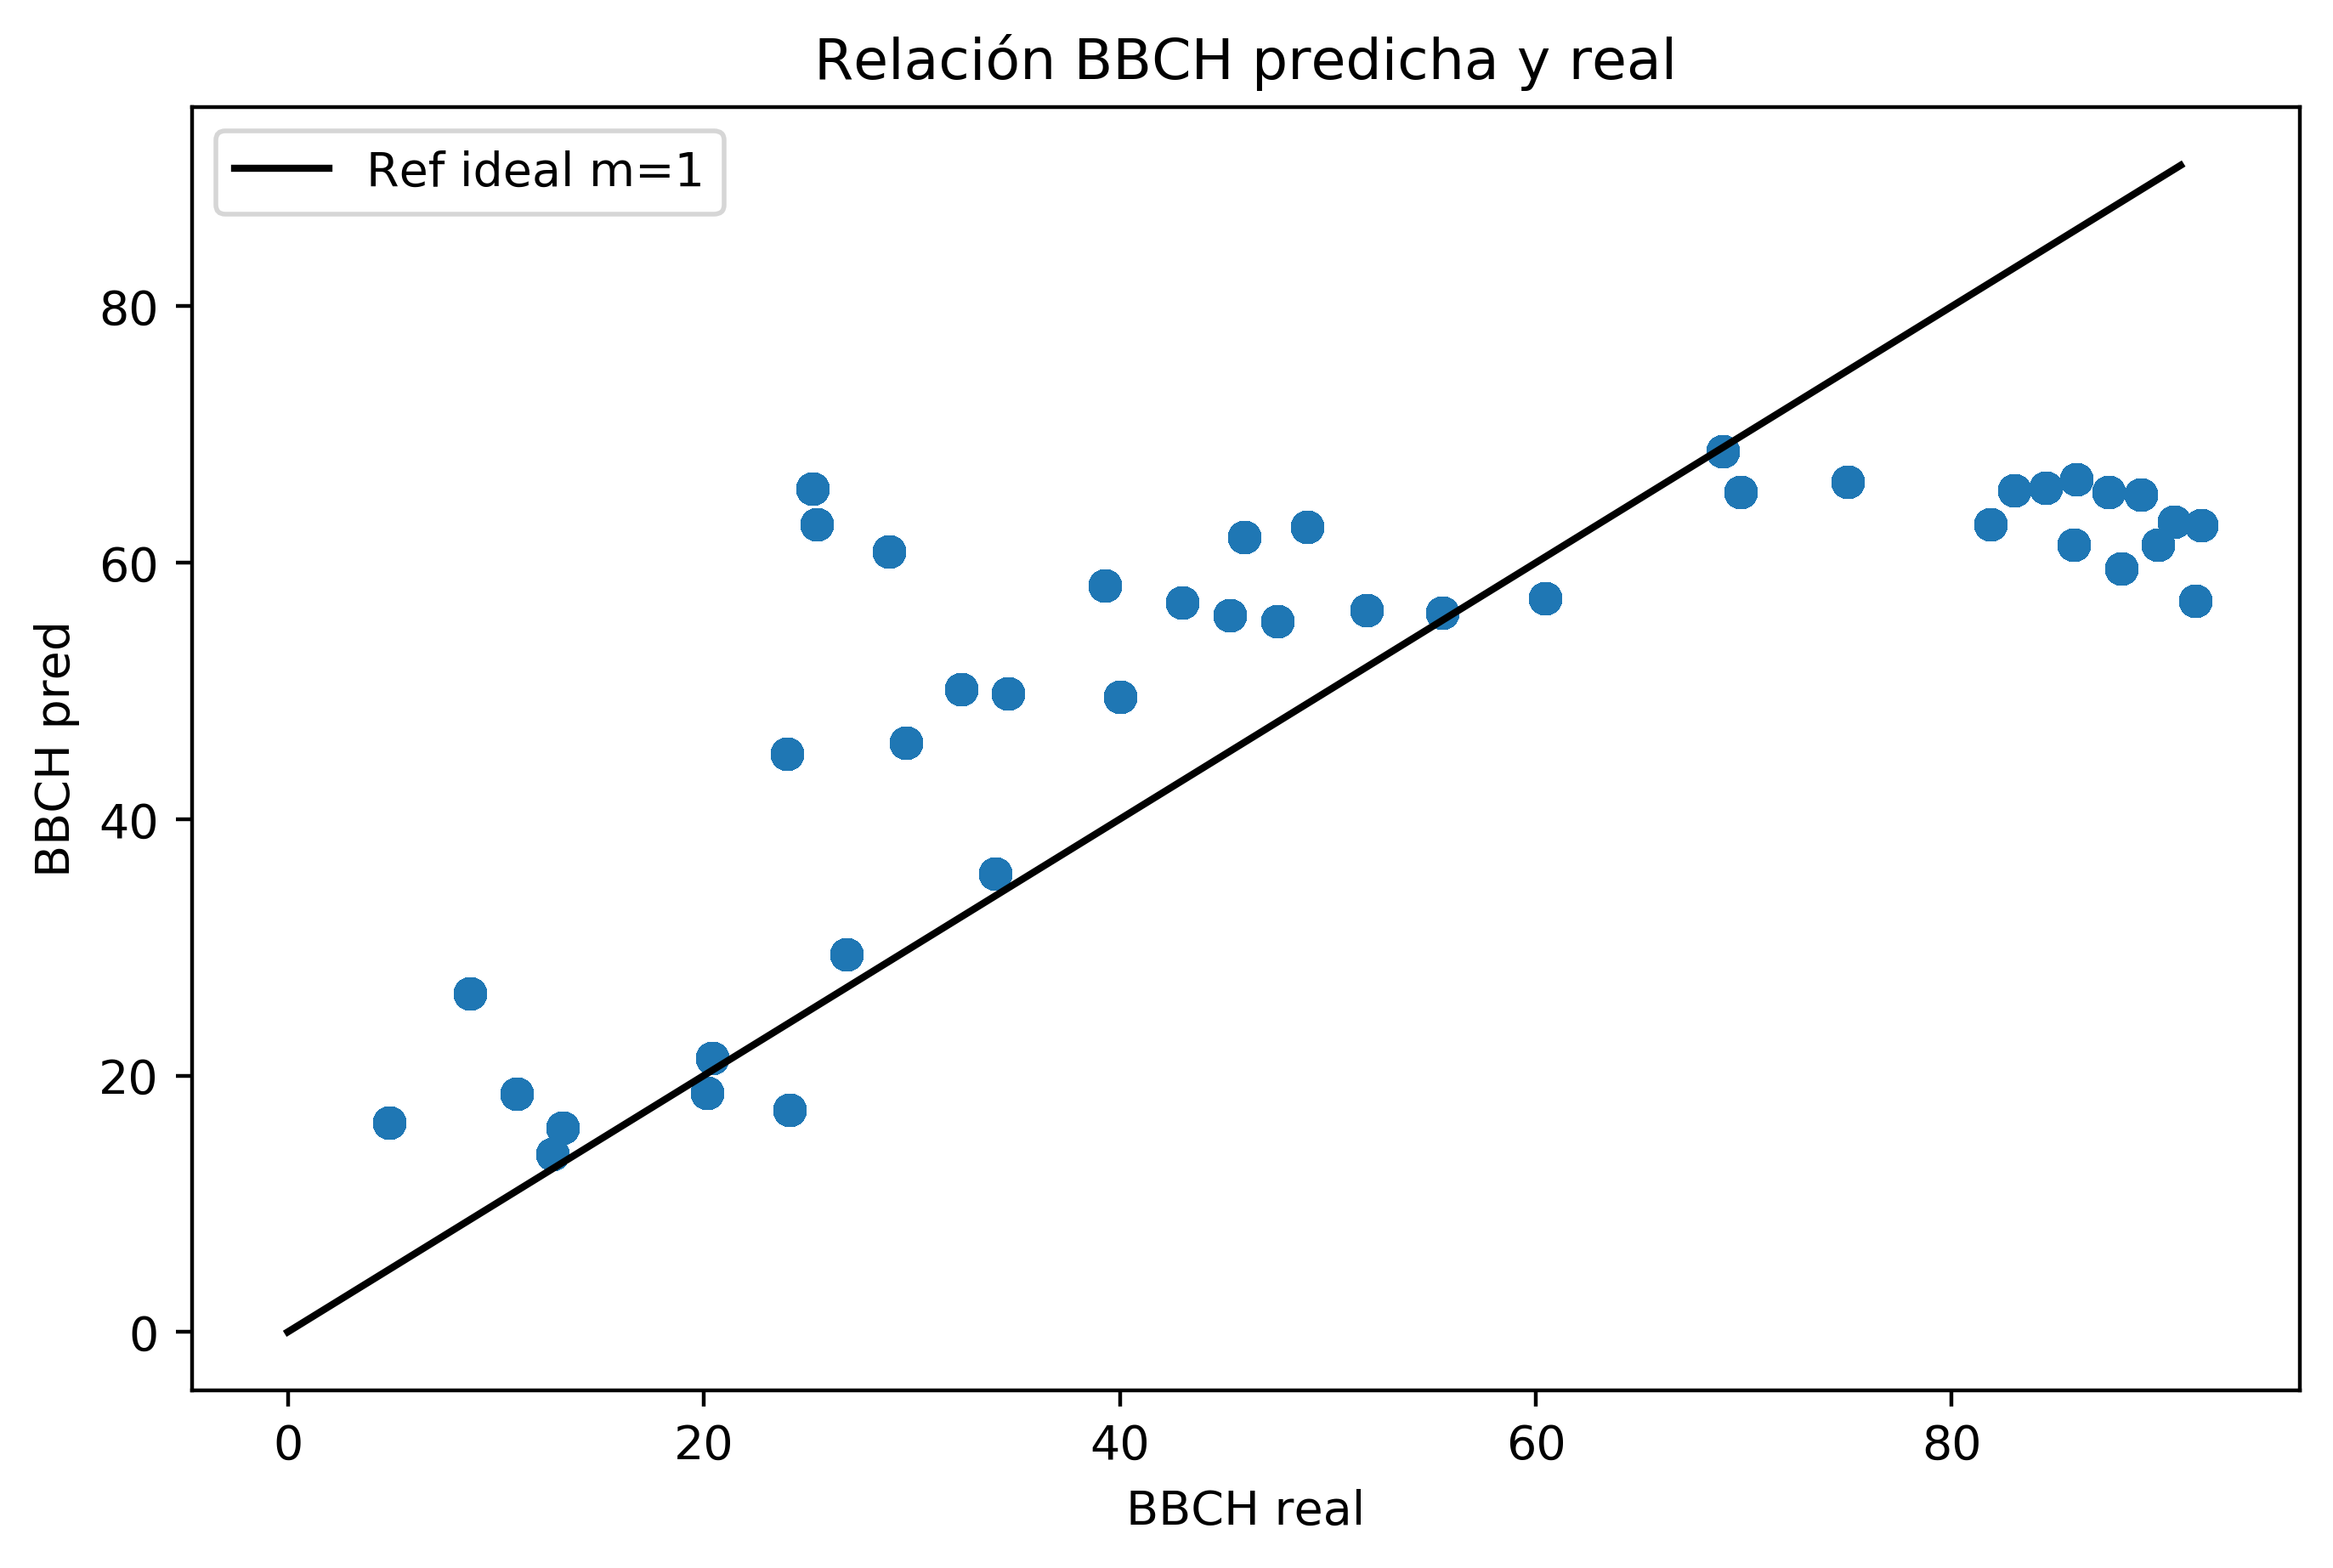
\includegraphics[width=0.95\linewidth]{archivos/tfg/Pixel/BBCHH_RELACION_BIEN_b}
  \caption{Relación de la salida predicha y la verdad de tierra del modelo de doble salida para la estimación de \gls{bbch}. \label{fig:p_rel_bh_b}}
\end{subfigure}
\begin{subfigure}{0.7\textwidth}
  \centering
  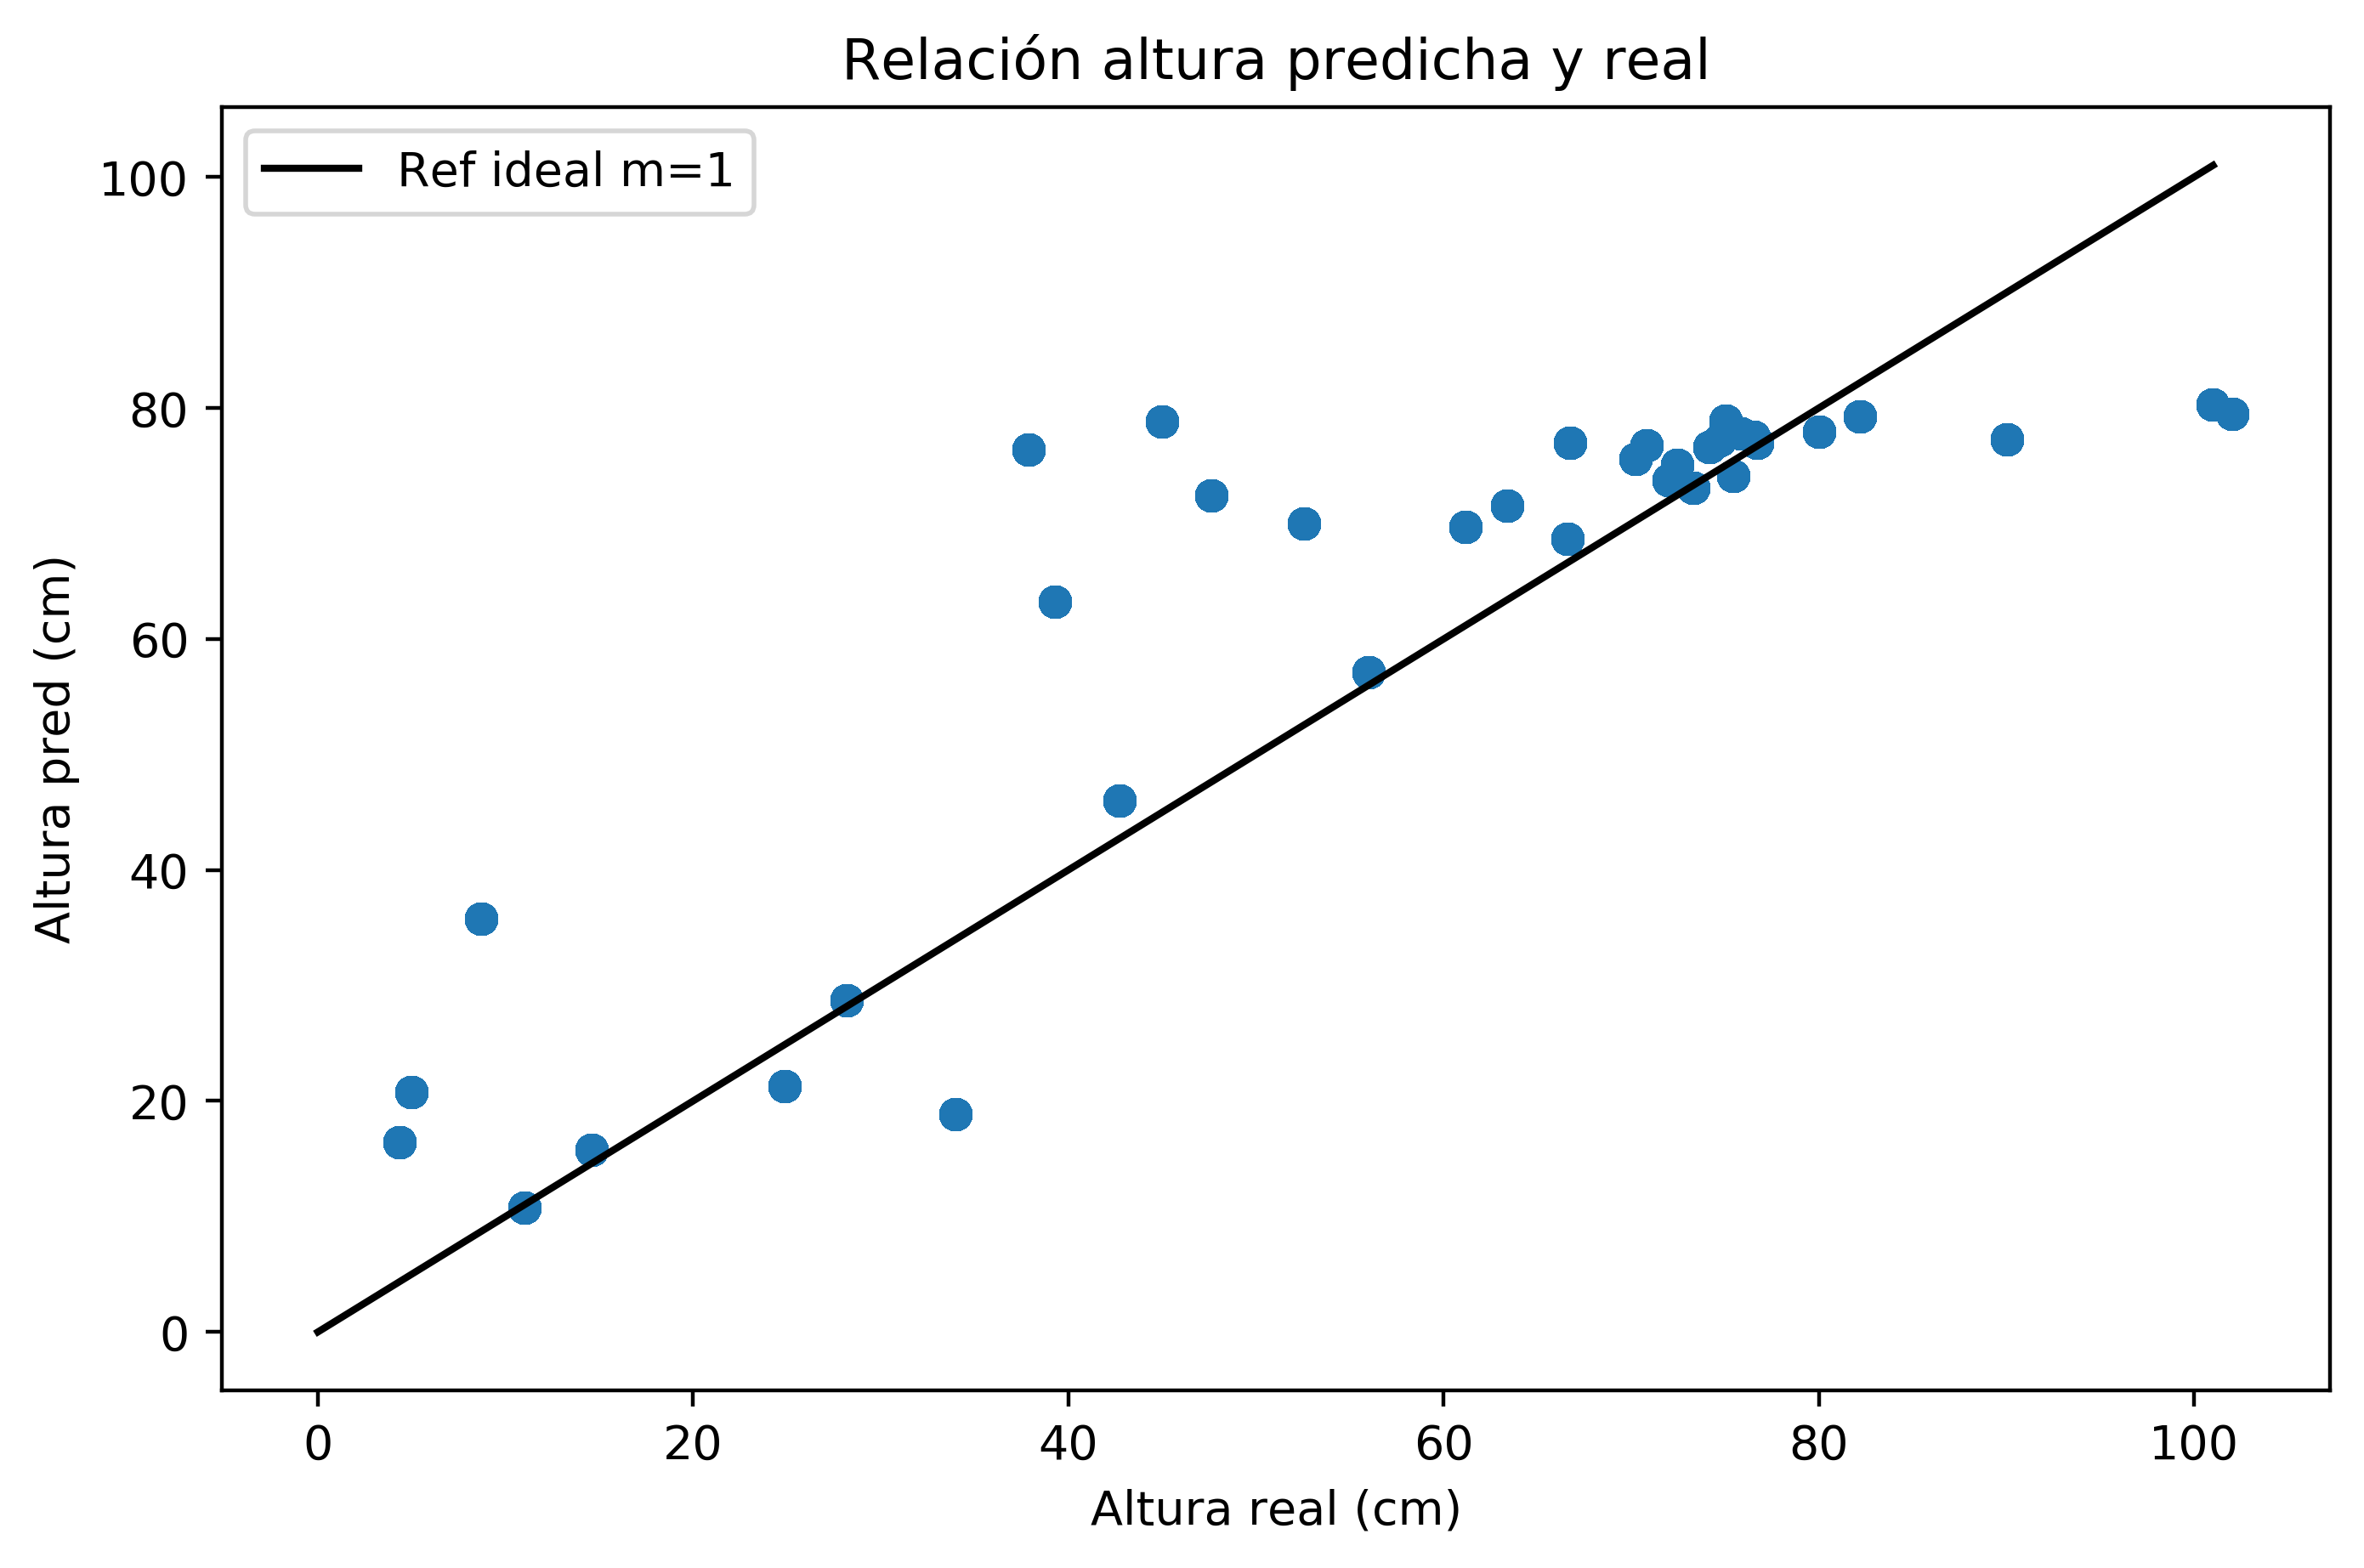
\includegraphics[width=0.95\linewidth]{archivos/tfg/Pixel/BBCHH_RELACION_BIEN_H}
  \caption{Relación de la salida predicha y la verdad de tierra del modelo de doble salida para la estimación de la altura\label{fig:p_rel_bh_h}}
\end{subfigure}
\caption{Relación de la salida predicha y la verdad de tierra del modelo de doble salida para la estimación de \gls{bbch} y la altura. \label{fig:p_rel_bh}}
\end{figure}
\par En todas las figuras se aprecia una distribución uniforme, lo cuál indica que se disponen de datos suficientes para cubrir las distintas etapas del desarrollo del cultivo. Solo se encuentran aglomeraciones de puntos en las figuras \ref{fig:p_rel_h} y \ref{fig:p_rel_bh_h}, las correspondientes a la variable altura, donde en las últimas etapas se mantiene una altura entorno a 70cm por más tiempo, por lo que se tienen más muestras. Además, las nubes de puntos se mantienen, en general, cercanos a la recta de referencia, exceptuando el pico de las etapas tempranas, presente en todos los casos, y las últimas etapas del cultivo, para las que la estimación es de nuevo inferior a la real, viéndose este error de predicción más severo para las figuras de \gls{bbch}, \ref{fig:p_rel_b} y \ref{fig:p_rel_bh_b}. Se sigue apreciando también en estas representaciones que la estimación de la altura para las etapas finales obtiene los mejores resultados. 
\\
\par Las diferencias entre los resultados expuestos en la figura \ref{fig:p_rel_2} y \ref{fig:p_rel_bh}, casos de salida individual y doble respectivamente, son difícilmente apreciables por la similitud de los modelos, y por tanto, de sus salidas. Se puede concluir entonces, que ambos modelos son eficientes y útiles en las estimaciones de \gls{bbch} y alturas, ya sea de manera individual o conjunta. 
\\ 
\par A parte de la evaluación con descriptores estadísticos que se realizan a la hora de comparar los dos métodos, se realiza una evaluación de los datos de entrada utilizados. La tabla \ref{tab:p_imp_f} representa el peso que tiene cada una de las variables de entrada en el modelo generado para cada uno de los 3 casos tratados. 

\begin{table}[h]
\centering
\begin{tabular}{l|ccc}
               & \gls{bbch} & Altura & \gls{bbch}\&Altura \\ \hline \hline
VV             & 0.19 & 0.16   & 0.19         \\
VH             & 0.61 & 0.61   & 0.59         \\
Ratio VH/VV    & 0.19 & 0.23   & 0.22         
     
\end{tabular}
\caption{Influencia de los parámetros de entrada en el modelo de estimación. \label{tab:p_imp_f}}
\end{table}

\par Aunque aquí se encuentran algunas diferencias, más que en la metodología anterior, todas son muy similares. El parámetro con más peso siempre es el coeficiente de backscattering VH, seguido por las otras dos variables aproximadamente igualadas. En esta metodología el parámetro principal tiene más peso, entorno a un 60\%, debido bien a la ausencia de las variables de entrada de desviación estándar, o bien al análisis a nivel de pixel, que obtenga mejores resultados gracias a esta variable. La razón por la que este parámetro funciona mejor como estimador se ha visto y comentado con las representaciones de la figura \ref{fig:rel_param}, totalmente válidas para este caso ya que las relaciones entre los datos de entrada y, por ejemplo, la \gls{bbch} son iguales.
%%%%%%%%%%%%%%%%%%%%%%%%%%%%%%%%%%%%%%%%%%%
%%%%%%%%%%%%%%%%%%%%%%%%%%%%%%%%%%%%%%%%%%%
%%%%%%%%%%%%%%%%%%%%%%%%%%%%%%%%%%%%%%%%%%%
\section{Comparativa de métodos}
\par La evaluación general de resultados realizada es la comparación entre los dos métodos de procesamiento de datos de entrada mencionados: a nivel de parcela o de pixel. En las siguientes tablas se pueden ver la evaluación de los resultados, divididos en entradas a nivel de parcela ~\ref{tab:errorpc} y a nivel de pixel ~\ref{tab:errorpx}, según los índices estadísticos de \gls{mae}, \gls{rmse} y el coeficiente de determinación ($R^2$). Ambos conjuntos corresponden al mejor caso de cada método, esto es, habiendo seleccionado sus parámetros de entrada óptimos en cuanto a número de variables y set de parcelas de entrenamiento, y habiendo optimizado también los parámetros del regresor.

\begin{table}[h]
\centering
\begin{tabular}{lccc}
\multicolumn{4}{c}{Datos de entrada a nivel de parcela}                            \\ \hline \hline
\multicolumn{1}{l|}{}                            & \gls{bbch}  & Altura & \gls{bbch}\&Altura \\ \cline{2-4} 
\multicolumn{1}{l|}{$R^2$}                       & 0.74  & 0.65   & 0.70 \\
\multicolumn{1}{l|}{\gls{rmse}} 				 & 15.39 & 17.87  & 15.69 \\
\multicolumn{1}{l|}{\gls{mae}}  				 & 11.13 & 14.21  & 12.63       
\end{tabular}
\caption{Índices estadísticos de las predicciones con datos de entrada a nivel de parcela. \label{tab:errorpc}}
\end{table}

\begin{table}[h]
\centering
\begin{tabular}{lccc}
\multicolumn{4}{c}{Datos de entrada a nivel de pixel}                            \\ \hline \hline
\multicolumn{1}{l|}{}                            & \gls{bbch}  & Altura & \gls{bbch}\&Altura \\ \cline{2-4} 
\multicolumn{1}{l|}{$R^2$}                       & 0.45  & 0.52   & 0.45         \\
\multicolumn{1}{l|}{\gls{rmse}} 				 & 22.23 & 19.89  & 21.17        \\
\multicolumn{1}{l|}{\gls{mae}}  				 & 17.26 & 15.64  & 16.58       
\end{tabular}
\caption{Índices estadísticos de las predicciones con datos de entrada a nivel de pixel.\label{tab:errorpx}}
\end{table}

\par Como se puede observar, para las 3 posibles salidas para las que se han diseñado los modelos, el método que emplea datos de entrada a nivel de parcela consigue notablemente mejores resultados. Se obtienen valores de coeficiente de determinación más cercanos a 1, valor ideal, apreciándose en el modelo de predicción de \gls{bbch} una mejora para el caso de parcelas de un 64.4\% con respecto al de pixel. Lo mismo ocurre en los índices de error, cuyo valor óptimo es 0: se obtienen valores inferiores para el método a nivel de parcela en todos los casos estudiados.
\\
\par Los mejores resultados obtenidos para el procesamiento a nivel de parcelas pueden recaer en que todos los datos recogidos de verdad de tierra se presentan por parcelas, por lo que no existen unos datos para contrastar cada pixel extraído de la información de satélite con el terreno. Dentro de cada parcela el cultivo no tiene porqué desarrollarse de manera homogénea, pero la información recibida de este consta del valor de \gls{bbch} (con el requisito de ser el correcto para al menos el 50\% del cultivo) y la altura generalizados por parcela, además de los máximos y mínimos de cada uno, por lo que las variaciones que se puede hallar en distintas zonas del cultivo no se tienen en cuenta. Por ello, el método de pixel implementado asigna un solo valor de salida para conjuntos de píxeles de la misma parcela, los cuales pueden estar representando unos niveles de \gls{bbch} o altura distintos, y esto conlleva un ajuste del modelo erróneo y, por tanto, peores índices estadísticos de evaluación. Aún así, este método no ha sido descartado, ya que el análisis a nivel de pixel es de gran interés para detectar esas variaciones de desarrollo de un cultivo dentro de una misma parcela. 		% Plantilla: Se muestran gráficas
%%%%%%%%%%%%%%%%%%%%%%%%%%%%%%%%%%%%%%%%%%%%%%%%%%%%%%%%%%%%%%%%%%%%%%%%
% Plantilla TFG/TFM
% Escuela Politécnica Superior de la Universidad de Alicante
% Realizado por: Jose Manuel Requena Plens
% Contacto: info@jmrplens.com / Telegram:@jmrplens
%%%%%%%%%%%%%%%%%%%%%%%%%%%%%%%%%%%%%%%%%%%%%%%%%%%%%%%%%%%%%%%%%%%%%%%%

\chapter{Conclusiones}
\label{conclusiones}
	% Plantilla: Se muestran matemáticas

%%%%
% CONTENIDO. BIBLIOGRAFÍA.
%%%%
\nocite{*} %incluye TODOS los documentos de la base de datos bibliográfica sean o no citados en el texto
\bibliography{bibliografia/bibliografia} % Archivo que contiene la bibliografía
\bibliographystyle{apacite}

%%%%
% CONTENIDO. LISTA DE ACRÓNIMOS. Comenta las líneas si no lo deseas incluir.
%%%%
% Incluye el listado de acrónimos utilizados en el trabajo. 
\printglossary[style=modsuper,type=\acronymtype,title={Lista de Acrónimos y Abreviaturas}]
% Añade el resto de acrónimos si así se desea. Si no elimina el comando siguiente
\glsaddallunused 

%%%%
% CONTENIDO. Anexos - Añade o elimina según tus necesidades
%%%%
\appendix % Inicio de los apéndices
\input{anexos/anexo_I}
\input{anexos/anexo_2}
\input{anexos/anexo_3}

\end{document}
